%%%%%%%%%%%%%%
%% Run LaTeX on this file several times to get Table of Contents,
%% cross-references, and citations.

%% If you have font problems, you may edit the w-bookps.sty file
%% to customize the font names to match those on your system.

%% w-bksamp.tex. Current Version: Feb 16, 2012
%%%%%%%%%%%%%%%%%%%%%%%%%%%%%%%%%%%%%%%%%%%%%%%%%%%%%%%%%%%%%%%%
%
%  Sample file for
%  Wiley Book Style, Design No.: SD 001B, 7x10
%  Wiley Book Style, Design No.: SD 004B, 6x9
%
%
%  Prepared by Amy Hendrickson, TeXnology Inc.
%  http://www.texnology.com
%%%%%%%%%%%%%%%%%%%%%%%%%%%%%%%%%%%%%%%%%%%%%%%%%%%%%%%%%%%%%%%%

%%%%%%%%%%%%%
% 7x10
%\documentclass{wileySev}

% 6x9
\documentclass{wileySix}

\usepackage{graphicx}
\usepackage{listings}
\usepackage{float}
\usepackage[urlcolor=blue, colorlinks=true]{hyperref}
\usepackage{color}
\usepackage{textcomp}

\definecolor{codegreen}{rgb}{0,0.6,0}
\definecolor{codegray}{rgb}{0.5,0.5,0.5}
\definecolor{codepurple}{rgb}{0.58,0,0.82}
\definecolor{backcolour}{rgb}{0.95,0.95,0.92}

\lstdefinestyle{mystyle}{
    backgroundcolor=\color{backcolour},
    commentstyle=\color{codegreen},
    keywordstyle=\color{magenta},
    numberstyle=\tiny\color{codegray},
    stringstyle=\color{codepurple},
    basicstyle=\footnotesize,
    breakatwhitespace=false,
    breaklines=true,
    captionpos=b,
    keepspaces=true,
    numbers=left,
    numbersep=5pt,
    showspaces=false,
    showstringspaces=false,
    showtabs=false,
    tabsize=2,
    language=sh
}

\lstset{style=mystyle}

%%%%%%%
%% for times math: However, this package disables bold math (!)
%% \mathbf{x} will still work, but you will not have bold math
%% in section heads or chapter titles. If you don't use math
%% in those environments, mathptmx might be a good choice.

% \usepackage{mathptmx}

% For PostScript text
\usepackage{w-bookps}

%%%%%%%%%%%%%%%%%%%%%%%%%%%%%%%%%%%%%%%%%%%%%%%%%%%%%%%%%%%%%%%%
%% Other packages you might want to use:

% for chapter bibliography made with BibTeX
% \usepackage{chapterbib}

% for multiple indices
% \usepackage{multind}

% for answers to problems
% \usepackage{answers}

%%%%%%%%%%%%%%%%%%%%%%%%%%%%%%
%% Change options here if you want:
%%
%% How many levels of section head would you like numbered?
%% 0= no section numbers, 1= section, 2= subsection, 3= subsubsection
%%==>>
\setcounter{secnumdepth}{3}

%% How many levels of section head would you like to appear in the
%% Table of Contents?
%% 0= chapter titles, 1= section titles, 2= subsection titles,
%% 3= subsubsection titles.
%%==>>
\setcounter{tocdepth}{2}

%% Cropmarks? good for final page makeup
%% \docropmarks

%%%%%%%%%%%%%%%%%%%%%%%%%%%%%%
%
% DRAFT
%
% Uncomment to get double spacing between lines, current date and time
% printed at bottom of page.
% \draft
% (If you want to keep tables from becoming double spaced also uncomment
% this):
% \renewcommand{\arraystretch}{0.6}
%%%%%%%%%%%%%%%%%%%%%%%%%%%%%%

%%%%%%% Demo of section head containing sample macro:
%% To get a macro to expand correctly in a section head, with upper and
%% lower case math, put the definition and set the box
%% before \begin{document}, so that when it appears in the
%% table of contents it will also work:

\newcommand{\VT}[1]{\ensuremath{{V_{T#1}}}}

%% use a box to expand the macro before we put it into the section head:

\newbox\sectsavebox
\setbox\sectsavebox=\hbox{\boldmath\VT{xyz}}

%%%%%%%%%%%%%%%%% End Demo


\begin{document}


\booktitle{SIG (Sistem Informasi Geografis)}
\subtitle{Semester 5}

\authors{D4TI3A\\
\affil{Angkatan 2017}
%Floyd J. Fowler, Jr.\\
%\affil{University of New Mexico}
}

\offprintinfo{SIG (Sistem Informasi Geografis), First Edition}{D4TI3A}

%% Can use \\ if title, and edition are too wide, ie,
%% \offprintinfo{Survey Methodology,\\ Second Edition}{Robert M. Groves}

%%%%%%%%%%%%%%%%%%%%%%%%%%%%%%
%%
\halftitlepage

%\titlepage


\begin{copyrightpage}{2019}
%Survey Methodology / Robert M. Groves . . . [et al.].
%\       p. cm.---(Wiley series in survey methodology)
%\    ``Wiley-Interscience."
%\    Includes bibliographical references and index.
%\    ISBN 0-471-48348-6 (pbk.)
%\    1. Surveys---Methodology.  2. Social 
%\  sciences---Research---Statistical methods.  I. Groves, Robert M.  II. %
%Series.\\
%
%HA31.2.S873 2007
%001.4'33---dc22                                             2004044064
\end{copyrightpage}

\dedication{`Jika Kamu tidak dapat menahan lelahnya belajar,
Maka kamu harus sanggup menahan perihnya Kebodohan.'
~Imam Syafi'i~}

\begin{contributors}
\name{Rolly Maulana Awangga,} Informatics Research Center., Politeknik Pos Indonesia, Bandung,
Indonesia



\end{contributors}

\contentsinbrief
\tableofcontents
\listoffigures
\listoftables
\lstlistoflistings


\begin{foreword}
Sepatah kata dari Kaprodi, Kabag Kemahasiswaan dan Mahasiswa
\end{foreword}

\begin{preface}
Buku ini diciptakan bagi yang awam dengan flask sekalipun.

\prefaceauthor{R. M. Awangga}
\where{Bandung, Jawa Barat\\
Februari, 2019}
\end{preface}


\begin{acknowledgments}
Terima kasih atas semua masukan dari para mahasiswa agar bisa membuat buku ini 
lebih baik dan lebih mudah dimengerti.

Terima kasih ini juga ditujukan khusus untuk team IRC yang 
telah fokus untuk belajar dan memahami bagaimana buku ini mendampingi proses 
Intership.
\authorinitials{R. M. A.}
\end{acknowledgments}

\begin{acronyms}
\acro{ACGIH}{American Conference of Governmental Industrial Hygienists}
\acro{AEC}{Atomic Energy Commission}
\acro{OSHA}{Occupational Health and Safety Commission}
\acro{SAMA}{Scientific Apparatus Makers Association}
\end{acronyms}

\begin{glossary}
\term{git}Merupakan manajemen sumber kode yang dibuat oleh linus torvald.

\term{bash}Merupakan bahasa sistem operasi berbasiskan *NIX.

\term{linux}Sistem operasi berbasis sumber kode terbuka yang dibuat oleh Linus Torvald
\end{glossary}

\begin{symbols}
\term{A}Amplitude

\term{\hbox{\&}}Propositional logic symbol 

\term{a}Filter Coefficient

\bigskip

\term{\mathcal{B}}Number of Beats
\end{symbols}

\begin{introduction}

%% optional, but if you want to list author:

\introauthor{Rolly Maulana Awangga, S.T., M.T.}
{Informatics Research Center\\
Bandung, Jawa Barat, Indonesia}

Pada era disruptif  \index{disruptif}\index{disruptif!modern} 
saat ini. git merupakan sebuah kebutuhan dalam sebuah organisasi pengembangan perangkat lunak.
Buku ini diharapkan bisa menjadi penghantar para programmer, analis, IT Operation dan Project Manajer.
Dalam melakukan implementasi git pada diri dan organisasinya.

Rumusnya cuman sebagai contoh aja biar keren\cite{awangga2018sampeu}.

\begin{equation}
ABC {\cal DEF} \alpha\beta\Gamma\Delta\sum^{abc}_{def}
\end{equation}

\end{introduction}

%%%%%%%%%%%%%%%%%% Isi Buku %%%%%%%%%%%%%%%%%%
\chapter{Tugas Pertama}
%\section{Arjun Yuda Firwanda (1174008)}
\subsection{Pengertian}
Sistem Informasi Geografis merupakan sistem informasi yang secara khusus mengelola data yang memiliki spasial atau keruangan.

Secara ringkasnya sistem informasi geografis merupakan sistem komputer yang memiliki kemampuan untuk membangun, menyimpan, mengelola dan menampilkan informasi bereferensi geografis, contohnya sebuah data yang diidentifikasi menurut lokasinya.

Pengertian Sistem Informasi Geografis merupakan gabungan dari tiga unsur pokok.
\begin{itemize}
	\item Sistem merupakan sekumpulan objek.
	\item Sistem Informasi merupakan sistem antara manusia dan mesin untuk menyajikan informasi untuk mendukung suatu fungsi operasi, manajemen dan pengambilan keputusan.
	\item Geografi  merupakan pengertian yang mengenai tempat-tempat yang terletak di permukaan bumi dan informasi mengenai keterangan dan posisi yang terdapat di permukaan bumi.
\end{itemize}

\subsection{Sejarah}
Awal dikenalnya Sistem Informasi Geografis (Geogragis Informastion System) tidak lepas dari perkembangan dalam bidang teknologi. Pada awal 1960-an perkembangan teknologi digunakan untuk bidang diluar militer. Pada ahli meterologi, geologi dan geofisika mulai menggunakan komputer dalam pembuatan peta.

Tahun 1963 di Kanada muncul CGIS (Canada Geographic Information System) dan selanjutnya menjadi GIS pertama di dunia. Dua tahun kemudian di Amerika Serikat beroperasi sistem bernama MIDAS yang digunakan untuk memproses data-data sumber daya alam.

\subsection{Koordinat}
Sistem Koordinat, osisi suatu titik biasanya dapat dinyatakan dengan koordinat yang mengacu pada suatu sistem koordinat tertentu.

\begin{itemize}
	\item Lokasi Titik Nol dari Sistem Koordinat
Posisi suatu titik di permukaan bumi umumnya ditetapkan dalam/terhadap suatu sistem koordinat terestris. Titik nol dari sistem koordinat terestris ini dapat berlokasi di titik pusat massa bumi (sistem koordinat geosentrik), maupun di salah satu titik di permukaan bumi (sistem koordinat toposentrik).  
	\item Orientasi dari Sumbu-sumbu Koordinat
Posisi tiga-dimensi suatu titik di permukaan bumi umumnya dinyatakan dalam suatu sistem koordinat geosentrik. Tergantung dari parameter-parameter pendefinisi koordinat yang digunakan. Ada dua sistem koordinat yang umum digunakan, yaitu sistem koordinat Kartesian (X,Y,Z) dan sistem koordinat Geodetik (L,B,h).
\end{itemize}


\subsection{Data Geospasial}
Data geospasial adalah kumpulan fakta yang berupa informasi tentang ruang kebumian (geospasial) yang menunjukan lokasi atau posisi dari suatu tempat atau objek yang direpresentasikan pada sebuah garis titik koordinat. Data geospasial dibagi menjadi 2 yaitu:

\begin{enumerate}
	\item Data Vector
Dalam bentuk data vector bagian objek dibumi ditampilkan sebagai kumpulan titik , garis dan polygon dimana sekumpulan tiitik yang saling terhubung akan membentuk garis dan garis yang saling terhubung antara titik awal dan titik akhir dengan nilai koordinat ynag sama akan membentuk polygon . Data vector dibagi menjadi 2 yaitu:

	\begin{itemize}
		\item Culture, memaparkan atau menampilkan data geospasial yang disertai dengan nama atribut atau memberikan keterangan atas nama dari objek di bumi. Contohnya nama dari suatu Negara, indicator batas air (keterangan kedalaman air laut), nama provinsi, daerah, wilayah dsb.
		\item Physical, memaparkan atau menampilkan data geospasial mengenai bentuk fisiknya atau gambaran tentang objek-objek alam yang ada dibumi. Contohnya gambaran laut, garis pantai, terumbu karang, danau dsb.
	\end{itemize}

	\item Data Raster, dapat menampilkan permukaan bumi seperti bentuk aslinya atau seperti dalam peta asli yang terlihat jelas dari setiap objek dengan keadaan alamnya. Data raster dibentuk agar menampilkan objek berupa elemen matriks atau grid, yang merepresentasikan objek dari data geospasial mengenai batas-batas yang berubah, ketinggian tanah.
\end{enumerate}

\subsection{Link}
\href{https://www.youtube.com/watch?v=HGscljVrxrE&feature=youtu.be}{Cek Di Youtubeku}

\subsection{Plagiarism}
\begin{figure}[Cek Plagiat]
	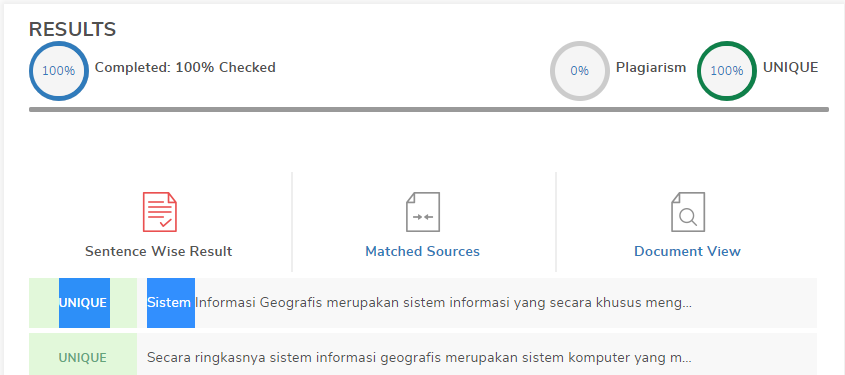
\includegraphics[width=4cm]{figures/1174008/pelagiat.png}
	\centering
	\caption{Cek Plagiat.}
\end{figure}

%\section{CHOIRUL ANAM (1174004)}
\subsection{Pengertian}
Geografi adalah ilmu yang mempelajari tentang lokasi serta persamaan dan perbedaan variasi keruangan atas fenomena fisik, dan manusia di atas permukaan bumi. Kata geografi berasal dari Bahasa Yunani yaitu gêo "Bumi", dan graphein "tulisan" atau "menjelaskan". Para sarjana, praktisi, atau penulis di bidang geografi disebut geograf atau geografer.Geografi juga merupakan nama judul buku bersejarah pada subjek ini, yang terkenal adalah Geographia tulisan Klaudios Ptolemaios pada abad kedua.Geografi lebih dari sekadar kartografi, studi tentang peta. Geografi tidak hanya menjawab apa, dan di mana di atas muka bumi, tapi juga mengapa di situ, dan tidak di tempat lainnya, kadang diartikan dengan "lokasi pada ruang." Geografi mempelajari hal ini, baik yang disebabkan oleh alam atau manusia. Juga mempelajari akibat yang disebabkan dari perbedaan yang terjadi itu.
Sistem informasi geografis (SIG) adalah sistem yang didesain untuk menangkap, menyimpan, mengolah, menganalisa, serta mempresentasikan data spasial.Dengan menghubungkan berbagai jenis data yang awalnya dianggap tidak berhubungan, SIG dapat membantu manusia dalam berbagai aspek pekerjaan. Proses menghubungkan ini umumnya dilakukan dalam konteks lokasi (spasial) dan waktu (temporal) yang sama.
\subsection{Sejarah}
Pada awalnya, peta hanya memiliki satu atau dua informasi saja didalamnya, sehingga jika seorang analis ingin mendapatkan informasi tambahan, dia harus melakukan overlay.Salah satu proses overlay pertama yang juga dianggap sebagai penggunaan analisa spasial pertama secara sukses adalah oleh John Snow di London pada tahun 1854. Dia melakukan pemetaan terhadap lokasi orang-orang yang mengidap penyakit cholera dan menghubungkannya dengan peta penyediaan air minum London.Pada awal abad ke-20, penggunaan teknik photozincography mulai meluas. Teknik ini memungkinkan peta terdiri dari beberapa layer yang nantinnya dapat diubah secara mandiri dari layer lainnya. Hal ini berguna untuk melakukan overlay dan analisa peta sesuai dengan layer yang dibutuhkan.Pada teknik ini, layer-layer yang ada dibuat dari film plastik atau lapisan kertas kalkir sehingga dapat digabungkan menjadi satu peta besar. Namun, teknik ini belum dapat dianggap sebagai SIG karena tidak terdapat database yang menghubungkan peta-peta tersebut.Pada tahun 1960, Canada mengembangkan sistem SIG pertamanya yang disebut CGIS atau Canada Geographic Information System. Sistem ini digunakan untuk menyimpan, mengolah, dan menganalisa informasi yang dimiliki oleh badan pertanahan Canada.
\subsection{Koordinat}
Peta, Proyeksi Peta, Sistem Koordinat, Survei dan GPS 
   Data spasial yang dibutuhkan pada SIG dapat diperoleh dengan berbagai cara. Salah satunya melalui survei dan pemetaan, yaitu penentuan posisi/koordinat di lapangan. Berikut ini akan dijelaskan secara ringkas beberapa hal yang berkaitan dengan posisi/koordinat serta metode-metode untuk mendapatkan informasi posisi tersebut di lapangan
\subsubsection{peta}
Peta adalah gambaran sebagian atau seluruh muka bumi baik yang terletak di atas maupun di bawah permukaan dan disajikan pada bidang datar pada skala dan proyeksi tertentu (secara matematis). Karena dibatasi oleh skala dan proyeksi maka peta tidak akan pernah selengkap dan sedetail aslinya (bumi). Untuk itu diperlukan penyederhanaan dan pemilihan unsur yang akan ditampilkan pada peta.
\subsubsection{proyeksipeta}
Pada dasarnya bentuk bumi tidak datar, tapi mendekati bulat. Maka untuk menggambarkan sebagian muka bumi untuk kepentingan pembuatan peta, perlu dilakukan langkah-langkah agar bentuk yang mendekati bulat tersebut dapat didatarkan dan distorsinya dapat terkontrol. Caranya dengan melakukan proyeksi ke bidang datar.
\subsubsection{Yang menggunakan bidang proyeksi}
Bidang datar, Bidang kerucut, Bidang silinder
\subsubsection{Proyeksi Universal Tranverse Mercator}
Proyeksi UTM dibuat oleh US Army sekitar tahun 1940-an. Sejak saat itu proyeksi ini menjadi standar untuk pemetaan topografi
\subsubsection{Sistem kordinat UTM}
Untuk menghindari koordinat negatif, dalam proyeksi UTM setiap meridian tengah dalam tiap zone diberi harga 500.000 mT (meter timur). Untuk harga-harga ke arah utara, ekuator dipakai sebagai garis datum dan diberi harga 0 mU (meter utara). Untuk perhitungan ke arah selatan ekuator diberi harga 10.000.000 mU.

   Wilayah Indonesia (90° – 144° BT dan 11° LS – 6° LU) terbagi dalam 9 zone UTM. Artinya, wilayah Indonesia dimulai dari zone 46 sampai zone 54 (meridian sentral 93° – 141° BT).
\subsubsection{Metode penentuan posisi}
Metode penentuan posisi adalah cara untuk mendapatkan informasi koordinat suatu objek di lapangan, contohnya koordinat titik batas, koordinat batas persil tanah dan lain-lain. Metode penentuan posisi dapat dibedakan dalam dua bagian, yaitu metode penentuan posisi terestris dan metode penentuan posisi extra-terestris (satelit).
Pada metode terestris, penentuan posisi titik dilakukan dengan melakukan pengamatan terhadap target atau objek yang terletak di permukaan bumi. Beberapa contoh metode yang umum digunakan adalah:
metode poligon, metode pemikatan ke muka, metode pengikatan ke belakang dan lain lain.
\subsection{Data Geospasial}
\subsubsection{Data spasial}
Data spasial adalah data yang memiliki informasi lokasi pada data tersebut. Informasi lokasi ini umumnya berbentuk sistem koordinat baik itu koordinat geografis ataupun koordinat proyeksi.
Data spasial umumnya digunakan untuk menunjukkan lokasi dari suatu obyek/kenampakan pada dunia nyata.
Terdapat dua jenis data spasial yaitu vektor dan raster. Kedua jenis data ini memiliki perbedaan sifat dan kegunaannya. Oleh karena itu, penggunaannya sangat tergantung dengan kondisi dan hasil yang ingin dicapai.
\subsubsection{Data vektor}
Data vektor adalah data yang direpresentasikan dengan garis, titik, atau polygon. Data vektor dihasilkan dari digitasi data raster ataupun penggambaran langsung obyek dunia nyata pada peta. Oleh karena itu, data vektor lebih sulit dibuat dibandingkan dengan data raster.
\subsubsection{Data Raster}
Data raster adalah data yang direpresentasikan dengan piksel dalam sebuah grafik. Data raster dihasilkan langsung oleh foto udara maupun foto satelit. Oleh karena itu, secara umum, data raster lebih mudah dibuat dibandingkan dengan data vektor.
\subsubsection{Data Aspasial}
Data aspasial adalah data yang tidak memiliki informasi mengenai lokasi data tersebut. Data ini umumnya digunakan untuk membantu menjelaskan informasi yang terkandung pada data spasial.
Contoh data aspasial adalah data atribut suatu obyek. Misal pada suatu peta terdapat titik berwarna hitam pada koordinat tertentu, kita tidak akan tahu titik tersebut bermakna apa tanpa adanya penjelas yaitu legenda. Legenda adalah salah satu contoh data aspasial.
Sistem informasi geografis modern menggunakan data digital untuk proses analisa dan Y666penafsirannya. Berikut ini adalah beberapa metode pengumpulan data untuk analisa SIG.
Digitasi adalah proses mendigitalkan data yang bersifat fisik. Hal ini perlu dilakukan karena mayoritas data perpetaan masih berada dalam bentuk fisik seperti pada lembaran film atau kertas peta.
Proses ini dapat dilakukan dengan cara memasukkan data fisik seperti foto dan peta kedalam mesin, atau men-scan data tersebut dan mendigitasinya secara manual dengan aplikasi.Proses digitasi akan mengubah data raster menjadi data vektor yang dapat diolah dan dianalisa oleh aplikasi SIG.
Survey juga merupakan bagian yang sangat penting dari SIG. Survey meliputi aktivitas pengambilan data langsung di tempatSurvey menghasilkan data yang nantinya dapat langsung dimasukkan kedalam basis data SIG dengan menggunakan coordinate geometry (COGO).Meskipun telah ada teknologi penginderaan jauh, survey masih sangat dibutuhkan dalam proses pemetaan. Hal ini disebabkan oleh keberadaan informasi-informasi detail lokasi yang mungkin tidak dapat ditangkap dan digambarkan oleh penginderaan jauh.
\subsection{https://youtu.be/QSoJBLX-hQ0}
\subsection{Plagiarism}
\begin{figure}[H]
	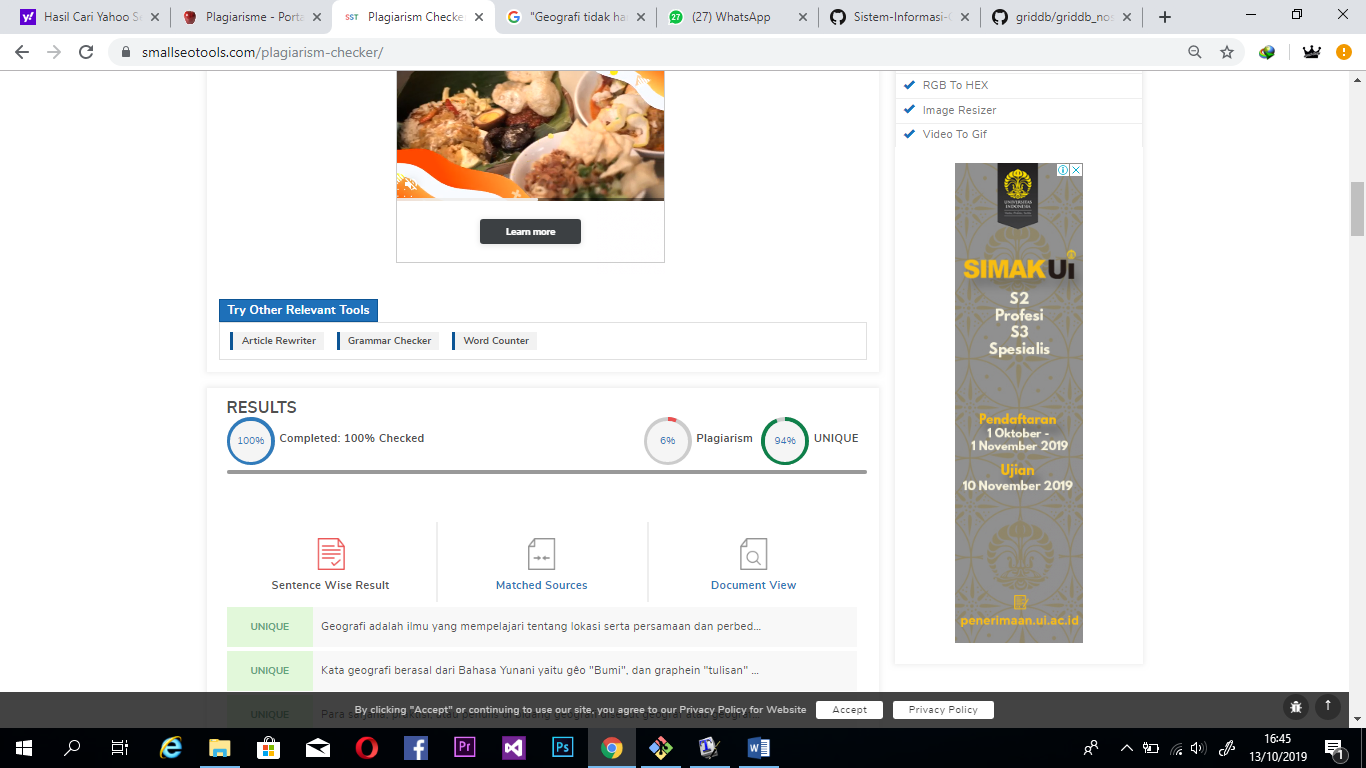
\includegraphics[width=4cm]{figures/1174004/choi.png}
	\centering
	\caption{plgt}
\end{figure}

%\section{Damara Benedikta (1174012)}
\subsection{Pengertian SIG}
SIG atau system informasi geografis merupakan sebuah system informasi yang berbasis computer dimana dirancang untuk dapat bekerja mengolah data yang memiliki informasi spasial. Didalam system tersebut dapat melakukan pengecekan, pengintegrasian, manipulasi,analisa dan menampilkan data secara spasial yang mereferensikan kondisi bumi

\subsection{Sejarah SIG}
Pada 35000 tahun yang lalu para pemburu diprancis mereka menggambar hewan pemangsa dan juga garis yang dipercya sebagai rute dari migrasi hewan hewan tersebut. Itu merupakan sebuah catatan awal pada system informasi geografis. 
awal abad 20 dimulailah pengembangan litografi foto yang mana peta dipisahakan beberapa lapisan (layer). Perkembangan perangkat keras komputer yang dipacu oleh penelitian senjata nuklir membawa aplikasi pemetaan menjadi multifungsi pada awal tahun 1960-an.
Sehingga pada tahun 1967 sebagai awal pengembangan  dari SIG yang  diterapkan di Ottawa, Ontario oleh Departemen Energi, Pertambangan dan Sumber Daya. SIG sendiri dikembangkan oleh Roger Tomlinson, yang kemudian disebut CGIS (Canadian GIS – SIG Kanada), yang memiliki kegunaan sebagai penympanan penganalisa dan pengolahan data yang telah dikumpulkan untuk inventarisasi tanah di Kanada.
Canadian GIS adalah system pertama yang berasal dari perbaikan aplikasi pemetaan yang dikembangkan oleh Roger Tomlinson yang disebut juga sebagai bapak SIG. Canadian GIS  sangat membutuhkan waktu lama dalam proses pengembangannya dan tidak dapat bersaing dengan aplikasi pemetaan yang lain. 
SIG berkembang seiring dengan ditemukannya komputer. Pada era perang dunia ke II, banyak kebutuhan  yang memicu perkembangan SIG guna membantu pemrosesan data untuk memenuhi kebutuhan militer.
Jack Dangermond yang belajar di labolatorium komputer grafik Harvard menemukan program Environmental Systems Research Institute (ESRI) Pada tahun 1969,  yang kemudian dikembangkan dan mampu menghasilkan software ArcInfo dan ArcView. Tahun 1970, SIG pertama kali digunakan oleh Roger Tomlinson dan Duane Marble. Dan juga pada tahun  1980 dan 1990, aplikasi SIG digunakan untuk berbagai kepentingan yang merambah ke banyak negara dengan berbagai model. Beberapa jenis aplikasi komersial dipublikasikan selama periode ini, seperti ArcView, MapInfo, ArcInfo, SMALLWORLD, SPANS GIS, INTERGRAPH dan PAMAP GIS.

\subsection{Koordinat}
Sitem koordinat merupakan posisi sebuah titik dimana dinyatakan dengan menggunakan 2 dimensi atau tiga dimensi yang mengacu pada sebuah system koordinat. Dalam sebuah titik koordinat mengacu pada 3 parameter dibawah: 
\begin{itemize}
	\item Lokasi Titik Nol dari Sistem Koordinat
Posisi suatu titik di permukaan bumi umumnya ditetapkan dalam/terhadap suatu sistem koordinat terestris. Titik nol dari sistem koordinat terestris ini dapat berlokasi di titik pusat massa bumi (sistem koordinat geosentrik), maupun di salah satu titik di permukaan bumi (sistem koordinat toposentrik).

	\item Orientasi dari Sumbu-sumbu Koordinat
	Dalam posisi tiga-dimensi (3D) suatu titik  yang dinyataan dalam suatu system koordinat geosentrik. Dimana tergantung jug pada setip parameternya. Jenis koordinat ada 2 yaitu koordinat kartesian dengan sumbu x,y dan z. 
	\begin{itemize}
	\item Latitude
	garis lintang mengarah dari khatulistiwa (0) ke kutub selatan, atau khatulistiwa ke kutub utara (sudut 0-90 dan 0 -90)

	\item Longitude
	merupakan garis bujur yang berarti sebuah  garis horizontal seperti dari khatulistiwa. Pada sudut 0 (Greenwich) ke arah Hawai adalah dari angka 0-180 drajat, sedangkan kebalikannya dari angka 0 ke -180

\end{itemize}
\end{itemize}
Titik 0 dimulai dari garis negara Inggris. Mengarah ke Indonesia akan menjadi angka positif. Kebalikannya koordinat Longitude minus adalah arah kebalikan.


\subsection{Data Geospasial}
Data Geospasial merupakan sebuah data mengenai lokasi geografis , dimensi ukuran atau karakteristik objek alam maupun objek buatan manusia yang berada dibawah ataupun diatas permukaan bumi . Pembahasan:
\begin{itemize}
	\item Satu
	Data sistem penentuan posisi global (GPS). Data GPS dikumpulkan melalui sistem navigasi radio berbasis satelit dan darat. Smartphone berkemampuan GPS dapat memberikan lokasi seseorang.

	\item Dua
	Data Penginderaan jauh melibatkan instrumen khusus yang menangkap data yang bisa diubah menjadi bentuk digital. Seperti halnya pada Satelit, pemindai, dan sistem radar adalah salah satu  contoh dari instrumen ini. Contoh lain dari penginderaan jauh adalah foto udara.

\end{itemize}
Dengan adanya data geospasial kita bisa melihat ruas jalan yang padat ataupun macet. Dengan mengetahui keadaan ini, bihak berwenang seperti polisi laku kintas dapat melakukan penanganan seperti pengalihan arus ke jalur alternatif atau pemberlakuan jalan satu arah.  

\subsection{Link}
\href {https://youtu.be/3P1zRqXBvx4}{klik disini}
\subsection{Plagiarism}
\begin{figure}[H]
	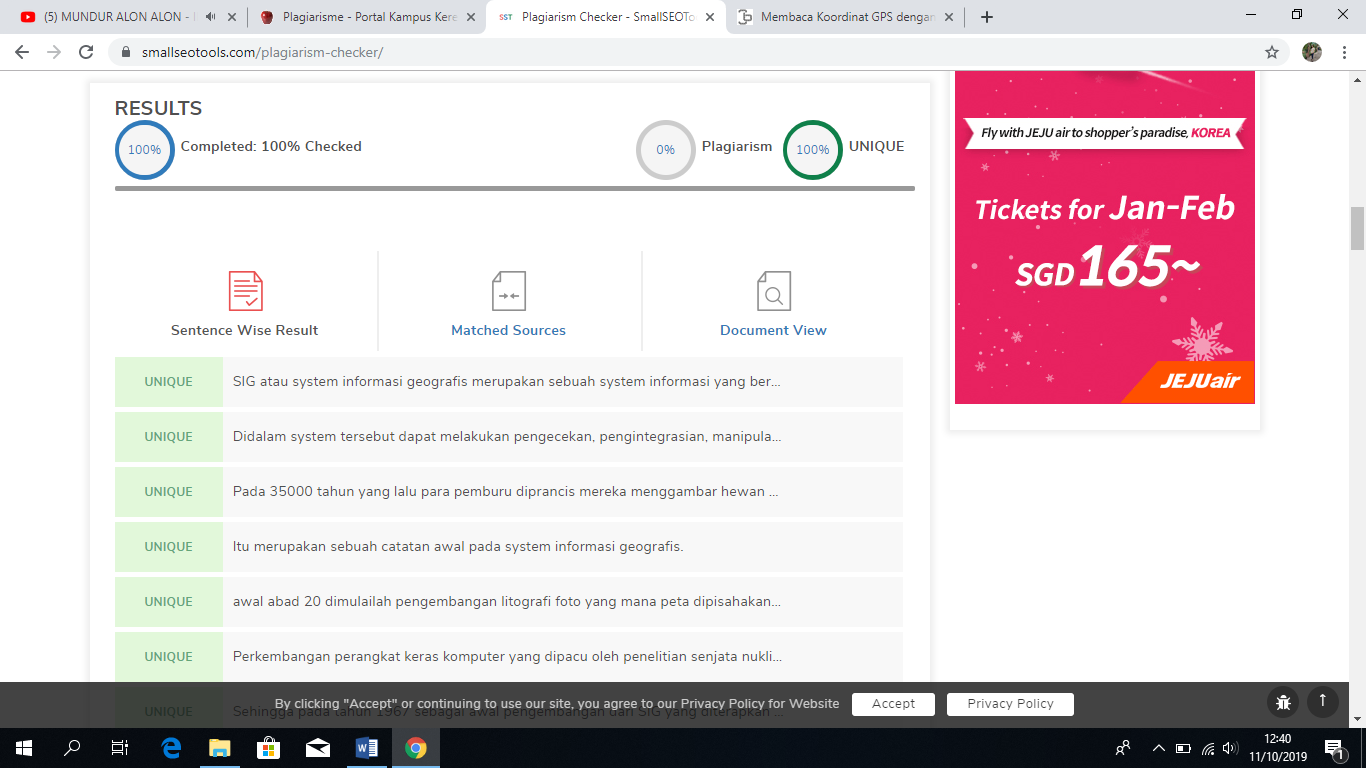
\includegraphics[width=4cm]{figures/1174012/gb.png}
	\centering
	\caption{Bukti}
\end{figure}
%\section{DEZHA AIDIL MARTHA (1174025)}
\subsection{Pengertian}
Geografi adalah suatu ilmu yang mempelajari dan mendalami tentang lokasi suatu sistem peta, serta persamaan dan perbedaan variasi keruangan atas fenomena fisik, dan manusia di atas permukaan bumi. Geografi berasal dari Bahasa Yunani yaitu gêo "Bumi", dan graphein "Gambaran" atau "Menjelaskan". Para sarjana, praktisi, atau penulis di bidang Geografi disebut Geograf atau Geografer.Geografi juga merupakan nama judul buku bersejarah pada subjek ini, yang terkenal adalah Geographia tulisan Klaudios Ptolemaios pada abad-2.Geografi lebih dari sekadar kartografi, studi tentang peta. Geografi bukan hanya membahas apa, dan di mana di atas muka bumi, tapi juga mengapa sesuatu ada di situ, dan tidak di tempat lainnya, kadang bisa diartikan dengan "lokasi pada ruang." Geografi mempelajari hal ini, baik yang disebabkan oleh alam atau manusia. Juga mempelajari akibat yang disebabkan dari perbedaan yang terjadi itu.\hfill\break
Sistem informasi geografis (SIG) adalah sistem yang didesain untuk menangkap, menyimpan, mengolah, menganalisa, serta mempresentasikan data spasial.Dengan menghubungkan berbagai jenis data yang awalnya dianggap tidak berhubungan, SIG dapat membantu manusia dalam berbagai aspek pekerjaan. Proses menghubungkan ini umumnya dilakukan dalam konteks lokasi (spasial) dan waktu (temporal) yang sama.
\subsection{Sejarah}
Pada awalnya, peta hanya memiliki satu atau dua informasi saja didalamnya, sehingga jika seorang analis ingin mendapatkan informasi tambahan, dia harus melakukan overlay.Salah satu proses overlay pertama yang juga dianggap sebagai penerapan analisa spasial pertama secara sukses adalah oleh ilmuan / Geografer John Snow di London pada tahun 1854. Dia melakukan pemetaan terhadap lokasi orang-orang yang mengidap penyakit cholera dan menghubungkannya dengan peta penyediaan air minum London.\hfill\break
Pada awal abad ke-20, penggunaan teknik photozincography mulai meluas. Teknik ini memungkinkan peta terdiri dari beberapa layer yang nantinnya dapat diubah secara mandiri dari layer lainnya. Hal ini berguna untuk melakukan overlay dan analisa peta sesuai dengan layer yang dibutuhkan.Pada teknik ini, layer-layer yang ada dibuat dari film plastik atau lapisan kertas kalkir sehingga dapat digabungkan menjadi satu peta besar. Akan tetapi, teknik ini belum dapat dianggap sebagai SIG karena tidak terdapat database yang menghubungkan peta-peta tersebut.Pada tahun 1960, Canada mengembangkan sistem SIG pertamanya yang disebut CGIS atau Canada Geographic Information System. Sistem ini digunakan untuk menyimpan, mengolah, dan menganalisa informasi yang dimiliki oleh badan pertanahan Canada.
\subsection{Koordinat}
Koordinat didapatkan dari hasil perpotongan antara garis latitude (Y) / lintang dan garis longitude(X) / garis bujur sehingga bisa menunjukan suatu lokasi pada suatu daerah. \hfill\break 
Umumnya koordinat dibedakan menajadi koordinat Geografi dan Universal Transver Mercator(UTM). Pada koordinat geografi dibedakan menajadi 3 yaitu : \hfill\break
\begin{itemize}
	\item Degree, Decimal(DD, DDDD) contoh S 4.56734 E 102.67235
	\item Degree,Minute(DD MM,MMMM) contoh S 4 42,5423’ E 105 34,6445’
	\item Degree, Minute, Second(DD MM SS,SS) contoh : S 4 43’ 45,22 E 103 33’ 33,25
\end{itemize}
\hfill\break
\begin{figure}[H]
	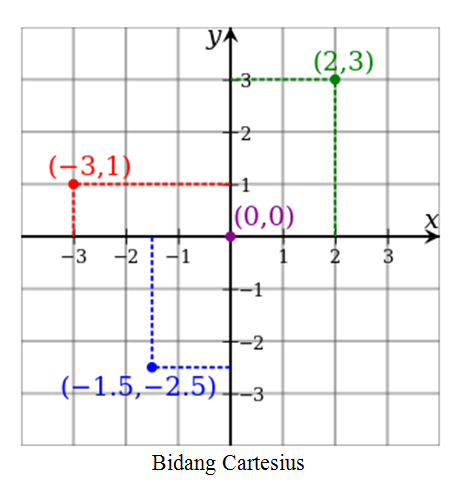
\includegraphics[width=4cm]{figures/1174025/1.png}
	\centering
	\caption{Contoh Koordinat}
\end{figure}
Pada system koordinat UTM biasanya terdapat pembagian waktu berdasarkan zonasinya. \hfill\break
\begin{figure}[H]
	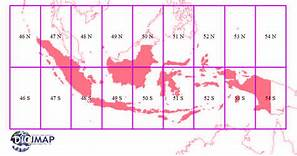
\includegraphics[width=4cm]{figures/1174025/2.jpg}
	\centering
	\caption{Contoh Koordinat UTM}
\end{figure}

\subsection{Data Geospasial}
Data geospasial merupakan pengambaran lokasi geografis,dimensi atau ukuran / karakteristik objek alam atau buatan manusia yang berada di bawah atau di atas permukaan bumi, data geospasial biasanya di singkat menjadi DG.
\hfill\break
Data Geospasial dibagi menjadi 3 yaitu :
\begin{itemize}
	\item Vektor
	Vektor merupakan salah jenis gambar yang dapat dibuat menggunakan aplikasi corel / adobe illustrator / aplikasi vektor lainnya. \hfill\break 
	Vektor itu sering digunakan untuk membuat gambar animasi dan vektor juga digunakan oleh goole maps.
	\item Roshen
	Roshen merupakan gambar yang di ambil dari satelit di luar angkasa, gambar ini biasanya bertipe jpg, dan pembaharuan data gambar ini berlangsung lama karena proses nya yang memakan waktu cukup banyak, jenis data ini digunakan oleh google earth.
	\item Roster
Data roster adalah data yang direpresentasikan dengan piksel dalam sebuah grafik. Data raster dihasilkan langsung oleh foto udara maupun foto satelit. Sehingga, secara umum, data roster lebih mudah dibuat dibandingkan dengan data vektor.
\end{itemize}

\subsection{Link}
\href{https://www.youtube.com/watch?v=Rw-D2J1h480}{Penjelasan GIT - Lalita Chandiany}
\subsection{Plagiarism}
\begin{figure}[H]
	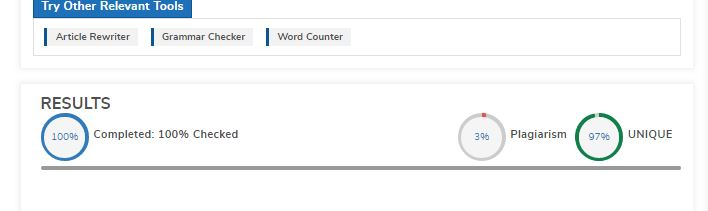
\includegraphics[width=4cm]{figures/1174025/plagiat.jpg}
	\centering
	\caption{Plagiat}
\end{figure}

%\section{Dwi Septiani Tsaniyah{1174003}}

\subsection{Pengertian}
Istilah pada sistem informasi sistem geografis adalah untuk digunakan sebagai pendekatan sebuah sistem yang digunakan dalam sistem informasi geografis , dengan lingkungan yang komponen nya terpisah-pisah,sistem yang digunakan untuk mempermudah pemahaman yang terintegrasi. Pada saat ini teknologi komputer sangat banyak digunakan oleh banyak orang jadi hampir semua sistem informasi nya berdasarkan dengan pada komputer.
Kata informasi berasal dari sebuah pengolahan sejumlah data, di dalam sistem informasi geografis informasi mempunyai volume yang sangat besa. Pada setiap objek geografi memiliki settingan data yang berbeda beda , data tersendiri karena tidak sepenuhnya data yang ada terdapat di dalam peta. Jadi semua data harus diasosiasikan terlebih dahulu untuk menjadi peta yang inteligent, pada data tersebut mampu menampilakn atau memberikan sebuah informasi dengan hanya mengklik mouse pada suatu objek.
Pada istilah geografi ini digunakan karena sistem informasi geografis yang dibangun secara berdasarkan pada geografi. Pada objek ini lebih mengarah pada sfesifikasi lokasi. Objek ini bisa berupa fisik,budaya ataupun ekonomi alamiah. Pada objek ini penampakan nya bisa dilihat didalam sebuah peta yang dimana untuk memberikan sebuah gambaran yang refresentatif dari suatu objek yang sesuai dengan kenyataan di bumi. Pada saat ini teknologi telah membantu proses pemetaan.

\subsection{Sejarah}
Sejarah geografi dimulai sejak manusia mulai berinteraksi dengan lingkunganya, hal ini juga merupakan awal mula dari berkembangnya ilmu pengetahuan tentang geografi.
Pada awal dikenalnya sistem informasi geografis bahwa tidak lepas dari adanya kemajuan didalam bidang teknologi. Pada awal tahun 1960 perkembangan sistem informasi geografis dalam ilmu komputer semakin pesat dan siap dingunakan pada bidang milliter. Pada taun 1700 teknik yang digunakan pada survei modern untuk pemetaan topografis digunakan atau diterapkan , hal ini juga termasuk pada versi awal pemetaan tematis.

\subsection{Koordinat}
Koordinat adalah suatu titik yang didapatkan dari hasil perpotongan dari garis latitude (lintang) dengan garis bujur (longitude) sehingga akan menunjukan lokasi pada suatu daerah. Umumnya koordinat dibedakan menjadi koordinat Geographic dan Universal Transver Mercator (UTM). Pada Koordinat Geogprahic dibedakan menjadi tiga berdasarkan satuannya yaitu :
Koordinat adalah suatu titik yang didapatkan dari hasil pemotongan sebuah garis lintang dengan garis bujur sehingga akan menunjukan sebuah lokasi pada suatu daerah. Pada Bujur/Longitude (X) merupakan garis yang perpindahannya secara vertical dan pada Lintang/Lattitude (Y) merupakan garis yang mempunyai perpindahan secara horizontal, pada (Gambar 1) menjelaskan perpotongan antara garis bujur dan garis lintang akan membentuk suatu titik pertemuan yang biasa disebut dengan titik koordinat.
dibedakan menajadi 3 yaitu : 
\begin{itemize}
	\item Degree, Decimal(DD, DDDD) contoh S 4.56734 E 102.67235
	\item Degree,Minute(DD MM,MMMM) contoh S 4 42,5423’ E 105 34,6445’
	\item Degree, Minute, Second(DD MM SS,SS) contoh : S 4 43’ 45,22 E 103 33’ 33,25
\end{itemize}
\hfill\break
\begin{figure}[H]
	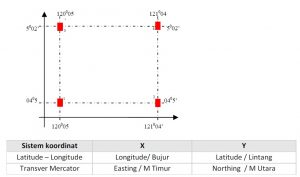
\includegraphics[width=4cm]{figures/1174003/koordinat.jpg}
	\centering
	\caption{Contoh Koordinat}
\end{figure}

\subsection{Data Geospasial}
Geospital data tentang suatu aspek fisik dari sebuah objek yang geografis , misalnya seperti bentuk alam tentu saja sungai,danau,pantai dan bentuk alam lainnya. Secara umun terdapat 2 fitur untuk menampilkan yaitu termasuk ke dalam geografis dan sistem informasi geospasial. Dalam struktur data yang demikian didalam nya ada unsur resolusi sebagai ukuran dari dimensi fitur geografis
Data Geospasial dibagi menjadi 2 yaitu :
\begin{itemize}
	\item Vektor
	Vektor merupakan salah jenis gambar yang dapat dibuat menggunakan aplikasi corel / adobe illustrator / aplikasi vektor lainnya.
	Vektor itu sering digunakan untuk membuat gambar animasi dan vektor juga digunakan oleh goole maps.
	\item Roshen
	Roshen merupakan gambar yang di ambil dari satelit di luar angkasa, gambar ini biasanya bertipe jpg, dan pembaharuan data gambar ini berlangsung lama karena proses nya yang memakan waktu cukup banyak, jenis data ini digunakan oleh google earth.
\end{itemize}
\subsection{Link}
\begin{itemize}
	\item \href{https://youtu.be/CXKVVDaUo30}{Materi GIS}
\end{itemize}
\subsection{Plagiarism}
\begin{figure}[H]
	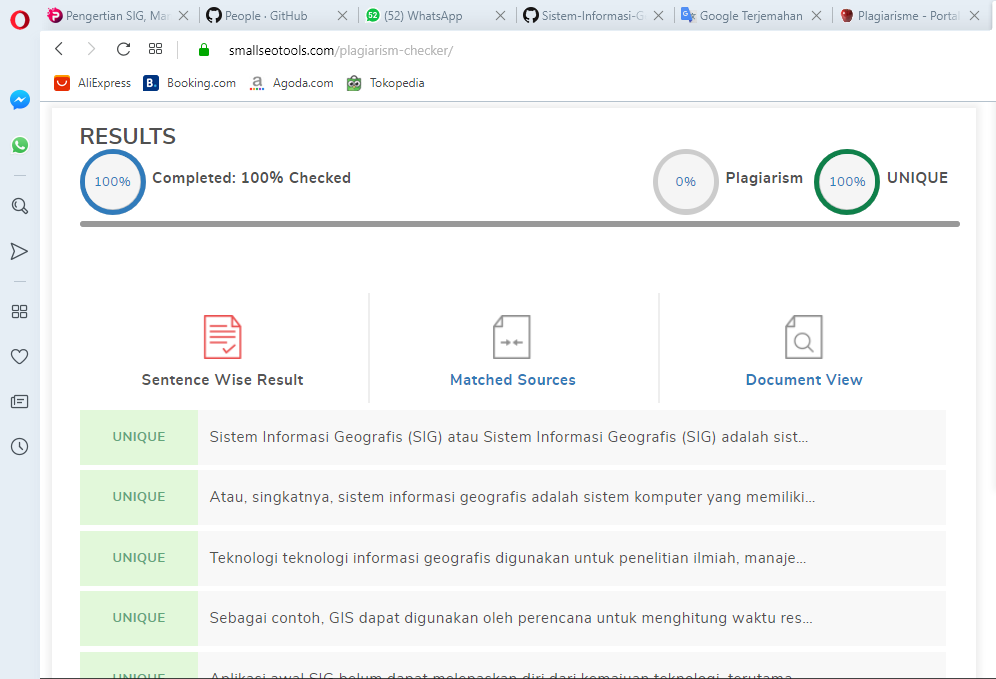
\includegraphics[width=4cm]{figures/1174003/1174003_plagiarisme.png}
	\centering
	\caption{Bukti Tidak Melakukan Plagiat}
\end{figure}
%\section{Dwi Yulianingsih(1174009)}
\subsection{Pengertian}
Sistem informasi geografis merupakan sebuah aplikasi /system pengolah data spasial yang memanfaatkan system komputerisasi dengan menggabungkan data grafis dan data atribut objek memanfaatkan peta dasar digital dengan referensi yang digunakan yaitu bumi. SIG pada dasarnya akan memunculkan dan memberi data-data yang diinginkan oleh user dimana dulunya manual yang diperbaharui menjadi data digital terkomputerisasi. System informasi geografis digunakan untuk mengumpulkan, mengubah, mengevaluasi, serta mengawasi seluruh data bumi yang dibutuhkan oleh user, dulunya data disimpan secara manual yang memungkinkan data bisa hilang/ rusak maka diperbaharui agar lebih mudah dan aman.

\subsection{Sejarah}
Sejarah dari SIG kurang lebih adalah sebagai berikut :
\begin{itemize}
\item Pada tahun 1960 ilmu computer mulai berkembang pesat dan siap digunakan untuk berbagai bidang. Ahli meteorology, geologi, dan 	geofisika mulai mengikuti perkembangan zaman dan memanfaatkannya  untuk membuat peta.
\item  Pada 1963 muncul Canadian geographic information system (CGIS) di Kanada dan menjadi system informasi geografis pertama di dunia. Dua tahun kemudian Amerika mulai mengikuti jejak Kanada dengan MIDAS-nya untuk memproses data SDA yang ada disana. 
\item Pada 1967 perkembangan awal SIG diterapkan di Ottawa, Ontario oleh departemen energi pertambangan dan sumber daya (ini merupakan perkembangan dari Canadian geographic information system yang digunakan untuk inventarisasi tanah Kanada (CLI) untuk mengetahui kemampuan memetakan informasi geologi disana).  
\item CGIS memiliki aplikasi pemetaan yang berkemampuan timpang susun atau overlay, perhitungan, pemindaian, system koordinat, dan topologi yang menyimpan atribut dan lokasional dalam berkas terpisah. CGIS ini bertahan sampai tahun 1970-an dan disempurnakan agar bisa bersaing dengan aplikasi pemetaan lain yang di keluarkan oleh vendor-vendor seperti Intergraph. 
\item Perkembangan yang terus menerus terjadi memacu pemtumbuhan SIG dapat dijalankan di workstation unix dan computer pribadi dengan standar platform yang lebih sedikit dan user yang mulai mengekplor data SIG lewat internet hingga bisa menjadi seperti sekarang.
\end{itemize}

\subsection{Koordinat}
Koordinat merupakan titik-titik yang didapat dari hasil pertemuan garis latitude dan longitude atau lintang dan bujur sehingga dapat menunjukan lokasi sebuah daerah/tempat. Pada umumnya koordinat dibedakan menjadi dua yaitu koordinat geograpik dan UTM. Di koordinat geograpik ada 3 satuan yaitu :
\begin{itemize}
\item Degree, Decimal (DD,DDDD) Contoh : S 3.56734 E 104.67235
\item Degree, Minute (DD MM,MMMM) Contoh : S 3' 43,5423' E 104 33,6445'
\item Degree, Minute, Second (DD MM SS,SS) Contoh : S 3' 43' 45,22'' E104 33' 33,25''
\end{itemize}

\begin{figure}[H]
	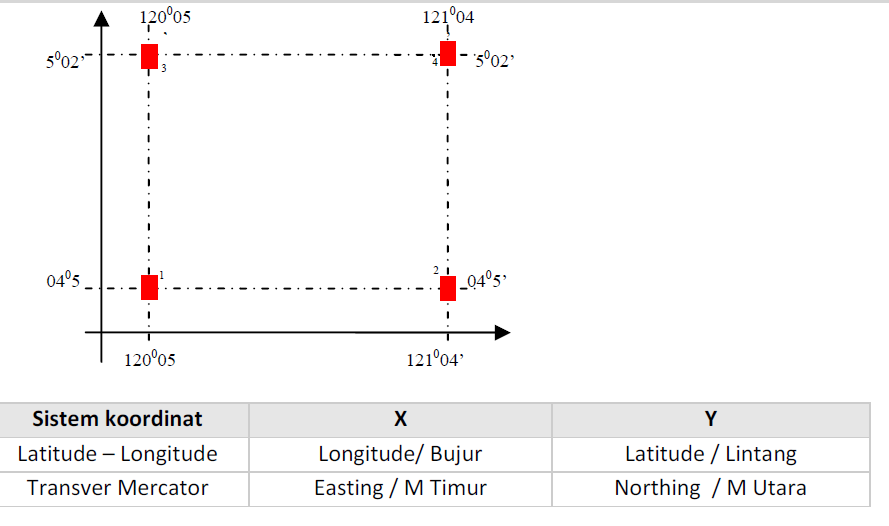
\includegraphics[width=5cm]{figures/1174009/t1.png}
	\centering
	\caption{geographic}
\end{figure}

Pada system UTM terbagi menjadi beberapa  waktu tergantung pada zonasinya, diindonesia waktu dibagi menjadi 16 zonasi seperti pada gambar di bawah :
\begin{figure}[H]
	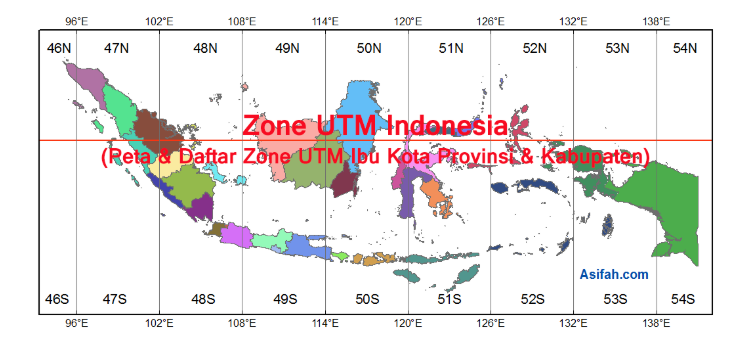
\includegraphics[width=5cm]{figures/1174009/t2.png}
	\centering
	\caption{UTM}
\end{figure}

\subsection{Data Geospasial}
Data geospasial adalah data yang memuat informasi spesifik mengenai fisik dan administrative dari sebuah objek. Aspek yang termasuk fisik disini seperti bentuk alam di permukaan (bumi) yang mengandung fenomena seperti jalan, rel kereta api, jembatan, bangunan dan sebagainya selain itu juga seperti aliran sungai, dataran tinggi, pantai, danau dan sebagainya. Termasuk juga aspek administrative seperti batas negara, pembagian wilayah, zona, postal code, batas tanah dan lainnya. Sebuah objek biasanya dikaitkan dengan atribut dari objeknya dan informasinya dapat di letakkan terpisah dengan pangkalan data induknya. Ada dua metode dalam data geospasial ini ada data vector dan data raster. Data vector terdiri dari gambaran titik geografis mau berupa titik, garis maupun polygon. Sementara data raster terdiri dari pixels yang digunakan untuk mrnggambarkan data yang berhubungan. 
\begin{figure}[H]
	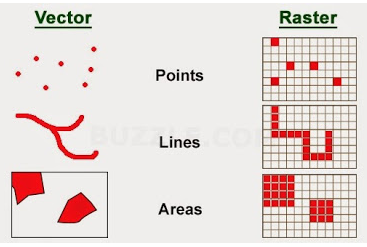
\includegraphics[width=5cm]{figures/1174009/t3.png}
	\centering
	\caption{geopasial}
\end{figure}

\subsection{Link Video}
\href{https://youtu.be/MXutHP_22_M}{Yuk lihat videonya}

\subsection{Plagiarism}
\begin{figure}[H]
	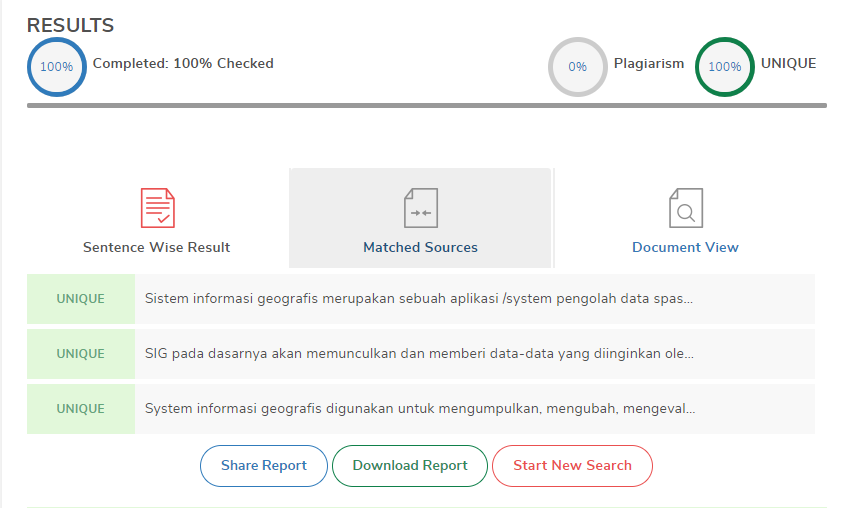
\includegraphics[width=5cm]{figures/1174009/plagiat1.png}
	\centering
	\caption{Bukti Tidak Plagiat}
\end{figure}

\begin{figure}[H]
	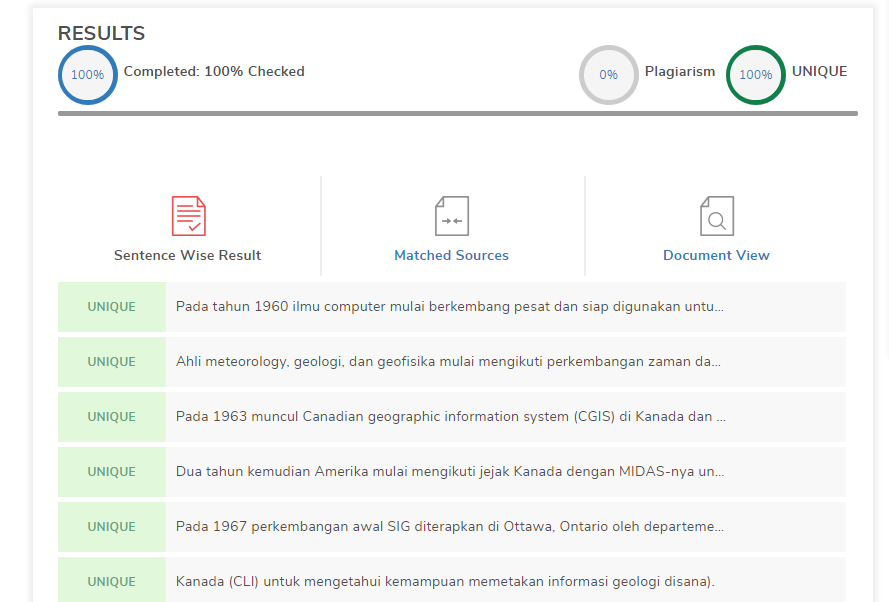
\includegraphics[width=5cm]{figures/1174009/plagiat2.png}
	\centering
	\caption{Bukti Tidak Plagiat}
\end{figure}

\begin{figure}[H]
	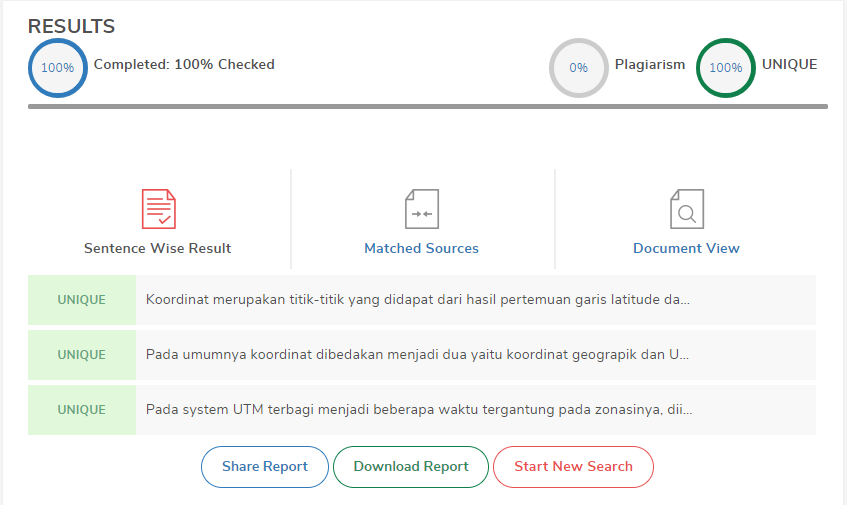
\includegraphics[width=5cm]{figures/1174009/plagiat3.png}
	\centering
	\caption{Bukti Tidak Plagiat}
\end{figure}

\begin{figure}[H]
	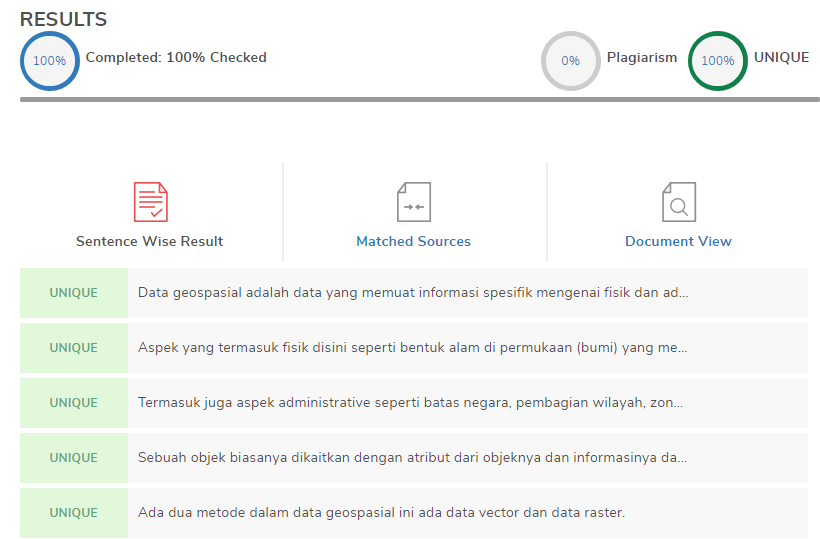
\includegraphics[width=5cm]{figures/1174009/plagiat4.png}
	\centering
	\caption{Bukti Tidak Plagiat}
\end{figure}

%\section{Evietania Charis Sujadi (1174051)}
\subsection{Pengertian}
adalah suatu sistem informasi yang berbasis komputer, dirancang untuk bekerja dengan menggunakan data yang memiliki informasi spasial . Sistem ini mengcapture, mengecek, mengintegrasikan, memanipulasi, menganalisa, dan menampilkan data yang secara spasial mereferensikan kepada kondisi bumi. \hfill\break
Aktifitas yang terjadi di bumi merupakan bagian dari ilmu Geografi.\hfill\break
\subsection{Sejarah}
pada 35000 tahun yang lalu, pada dinding gua Lascaux, Perancis, para pemburu Cro-Magnon menggambar hewan mangsa mereka, juga garis yang dipercaya sebagai rute migrasi hewan-hewan tersebut. pada catatan awal ini sejalan dengan dua elemen struktur pada sistem informasi gegrafis modern sekarang ini, arsip grafis yang terhubung ke database atribut.\hfill\break
Pada tahun 1700an sebuah teknik survey modern untuk pemetaan topografis diterapkan, termasuk versi awal pemetaan tematis, misalnya untuk keilmuan atau data sensus.\hfill\break
pada awal abad ke 20 memperlihatkan pengembangan “litografi foto” dimana peta dipisahkan menjadi beberapa lapisan . Perkembangan perangkat keras komputer yang dipacu oleh penelitian senjata nuklir membawa aplikasi pemetaan menjadi multifungsi pada awal tahun 1960an.\hfill\break
Pada tahub 1967 merupakan awal pengembangan SIG yang bisa diterapkan di Ottawa, Ontario oleh Departemen Energi, Pertambangan dan Sumber Daya. dikembangkan oleh roger dimana, kemudian disebut CGIS (Canadian GIS – SIG Kanada), digunakan untuk menyimpan, menganalisis dan mengolah data yang dikumpulkan untuk Inventarisasi Tanah Kanada (CLI) sebuah inisiatif untuk mengetahui kemampuan lahan di wilayah pedesaan Kanada dengan memetakaan berbagai informasi pada tanah, pertanian, pariwisata, alam bebas, unggas dan penggunaan tanah pada skala 1:250000.\hfill\break
CGIS bertahan sampai tahun 1970-an dan memakan waktu lama untuk penyempurnaan setelah pengembangan, dan tidak bisa bersaing denga aplikasi pemetaan komersil yang dikeluarkan beberapa vendor seperti Intergraph. Perkembangan perangkat keras mikro komputer memacu vendor lain seperti ESRI dan CARIS berhasil membuat banyak fitur SIG, menggabung pendekatan generasi pertama pada pemisahan informasi spasial dan atributnya, dengan pendekatan generasi kedua pada organisasi data atribut menjadi struktur database. Perkembangan industri pada tahun 1980 dan 1990 memacu sebuah pertumbuhan SIG pada workstation UNIX dan komputer pribadi. Pada akhir abad ke 20, pertumbuhan yang cepat di berbagai sistem dikonsolidasikan dan distandarisasikan menjadi platform lebih sedikit, dan para pengguna mulai mengekspor menampilkan data SIG lewat internet, yang membutuhkan standar pada format data dan transfer
\subsection{Koordinat}
Koordinat didapatkan dari hasil perpotongan antara garis latitude (Y) / lintang dan garis longitude(X) / garis bujur sehingga bisa menunjukan suatu lokasi pada suatu daerah.
\subsection{Data Geospasial}
Data yang aspek fisiknya dan administratif dari sebuah objek geografis. Aspek fisik di sini mencakup pula bentuk anthropogenic dan bentuk alam baik yang terdapat di permukaan maupun di bawah permukaan bumi. 
\subsection{Link}
\href{https://youtu.be/eby2SXgrvbU}{Pencet Aku}
\subsection{Plagiarism}
\begin{figure}[H]
	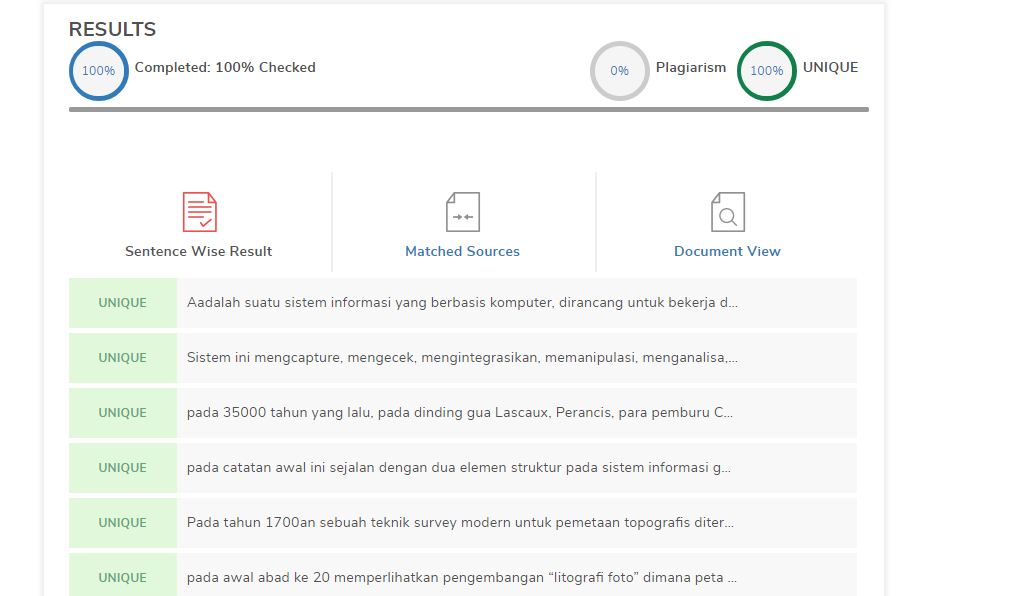
\includegraphics[width=4cm]{figures/1174051/1/1.png}
	\centering
	\caption{Bukti Tidak Melakukan Plagiat}
\end{figure}

\subsubsection{List}
\begin{enumerate}
	\item Satu
	\item Dua
\end{enumerate}

\begin{itemize}
	\item Satu
	\item Dua
\end{itemize}

\href{link kamu}{alias}
contoh link
\href{https://www.google.com/}{klik me}
%\section{Felix Setiawan Lase (1174026)}
\subsection{Pengertian}
Pada dasarnya istilah sistem informasi geografis adalah kombinasi dari tiga elemen utama yaitu sistem, informasi, dan geografi.
Sistem adalah kumpulan benda, ide, dan hubungan mereka dalam mencapai tujuan bersama.\hfill\break
Sistem informasi adalah sistem antara manusia dan mesin yang terintegrasi untuk menyajikan informasi untuk mendukung fungsi operasi, manajemen, dan pengambilan keputusan dalam organisasi.\hfill\break
Penggunaan istilah informasi geografis menyiratkan informasi tentang tempat-tempat yang terletak di permukaan bumi. Pengetahuan tentang posisi di mana objek berada di permukaan bumi dan informasi tentang informasi dan posisi yang terkandung di permukaan bumi.
\subsection{Sejarah}
Pengenalan awal GIS tidak lepas dari kemajuan di bidang teknologi, khususnya komputer. Selama perang dunia kedua pemrosesan data mengalami kemajuan pesat terutama untuk memenuhi kebutuhan militer dalam memprediksi lintasan balistik. Pada awal 1960-an perkembangan ilmu komputer berkembang pesat dan siap digunakan untuk bidang lain di luar militer. Ahli meteorologi, geologi dan geofisika mulai menggunakan komputer dalam pembuatan peta.\hfill\break

Pada tahun 1963 di Kanada muncul CGIS (Sistem Informasi Geografis Kanada), dan kemudian menjadi GIS pertama di dunia. Dua tahun kemudian di Amerika Serikat mengoperasikan sistem serupa yang disebut MIDAS yang digunakan untuk memproses data sumber daya alam.
\subsection{Koordinat}
Koordinat adalah titik yang diperoleh dari perpotongan garis lintang (garis lintang) dengan garis bujur (garis bujur) sehingga akan menunjukkan lokasi di suatu daerah. Secara umum koordinat dibagi menjadi Koordinat Geografis dan Universal Transver Mercator (UTM)
\subsection{Data Geospasial}
\begin{enumerate}
	\item Data global positioning system (GPS). Data GPS dikumpulkan melalui sistem navigasi radio berbasis satelit dan darat. Smartphone yang mampu GPS dapat memberikan lokasi seseorang.
	\item Data penginderaan jauh. Penginderaan jauh melibatkan instrumen khusus yang menangkap data yang dapat dikonversi menjadi bentuk digital. 
\end{enumerate}\hfill\break

Foto udara dapat digunakan untuk mengenali beberapa objek di muka bumi. Dengan menganalisis bentuk, ukuran dan warna benda-benda ini, kita dapat mengamati keberadaan tanah basah atau kering, tanaman atau penyakit yang sehat, dan sawah irigasi atau tadah hujan. Tanah basah akan lebih gelap jika dibandingkan dengan tanah kering.

Data geospasial banyak berguna, baik untuk bisnis maupun untuk pemerintah.\hfill\break

Sebagai contoh, dengan data geospasial kita dapat melihat jalan mana yang padat atau bahkan padat. Dengan mengetahui situasi ini, pihak berwenang seperti polisi dapat melakukan penanganan seperti mengalihkan arus ke rute alternatif atau menerapkan jalan satu arah.

\subsection{Link}
\begin{itemize}
	\item \href{https://youtu.be/GOjKvnfiYC8}{Lihat Disini}
\end{itemize}
\subsection{Plagiarism}
\begin{figure}[H]
	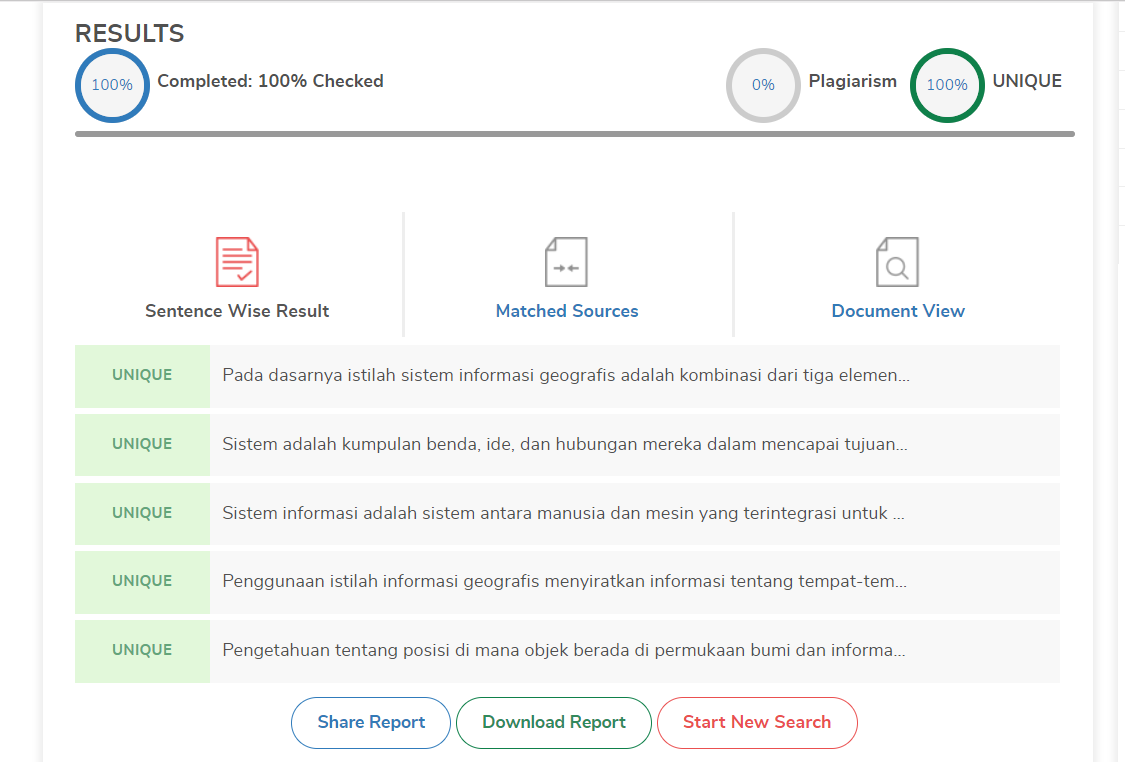
\includegraphics[width=4cm]{figures/1174026/1/1.png}
	\centering
	\caption{Bukti Tidak Melakukan Plagiat}
\end{figure}
\begin{figure}[H]
	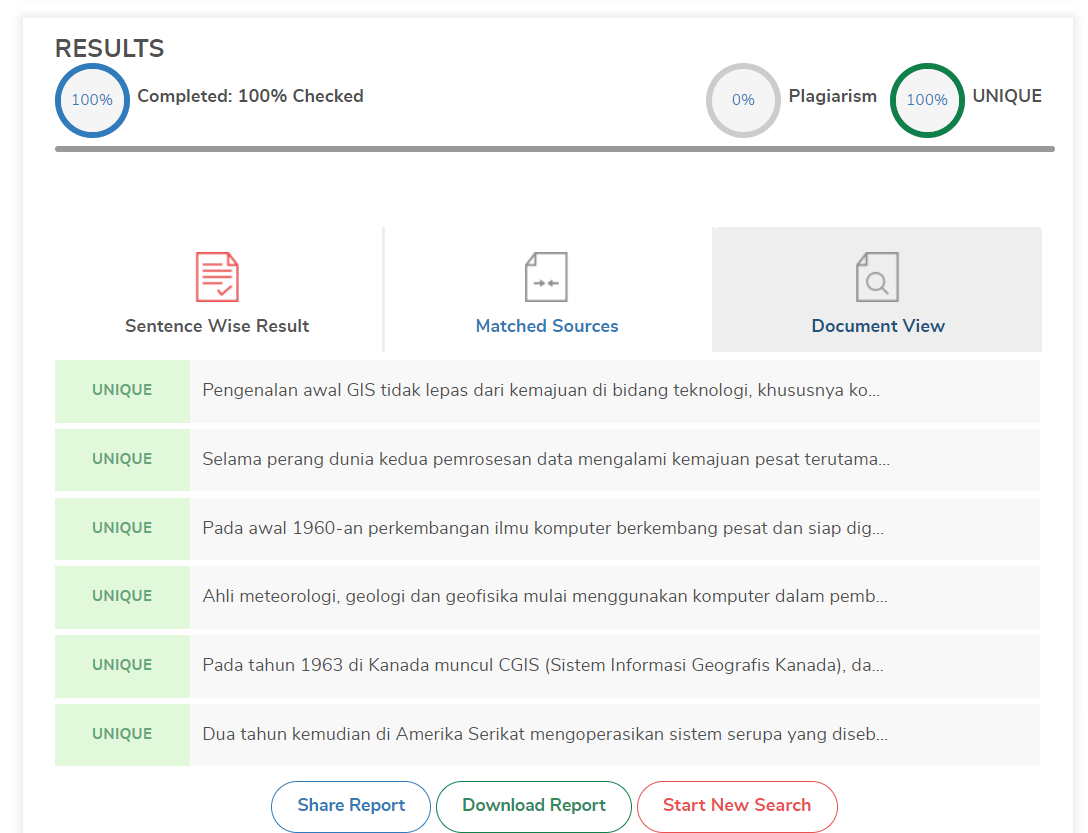
\includegraphics[width=4cm]{figures/1174026/1/2.png}
	\centering
	\caption{Bukti Tidak Melakukan Plagiat}
\end{figure}
\begin{figure}[H]
	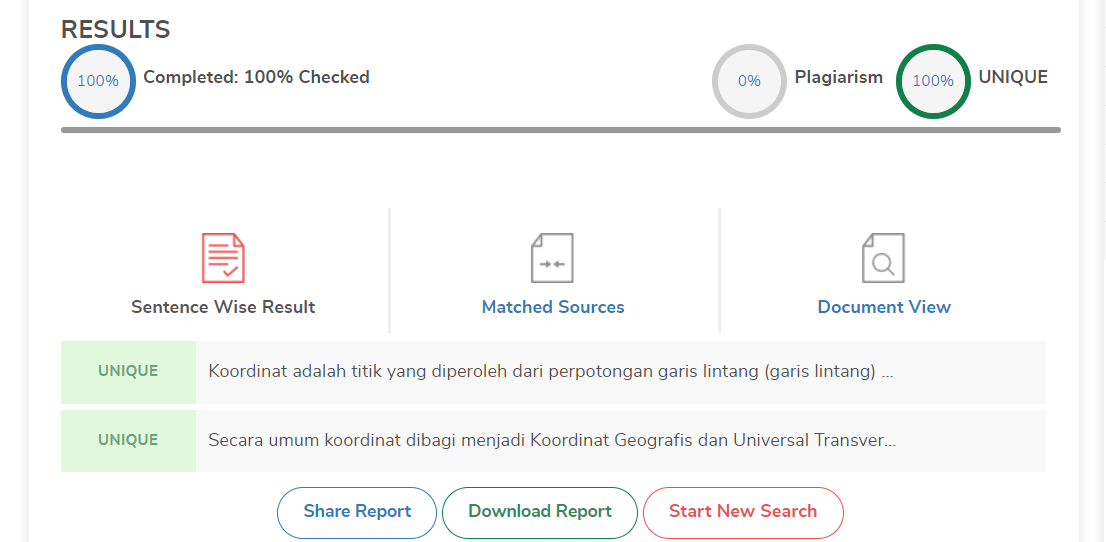
\includegraphics[width=4cm]{figures/1174026/1/3.png}
	\centering
	\caption{Bukti Tidak Melakukan Plagiat}
\end{figure}
\begin{figure}[H]
	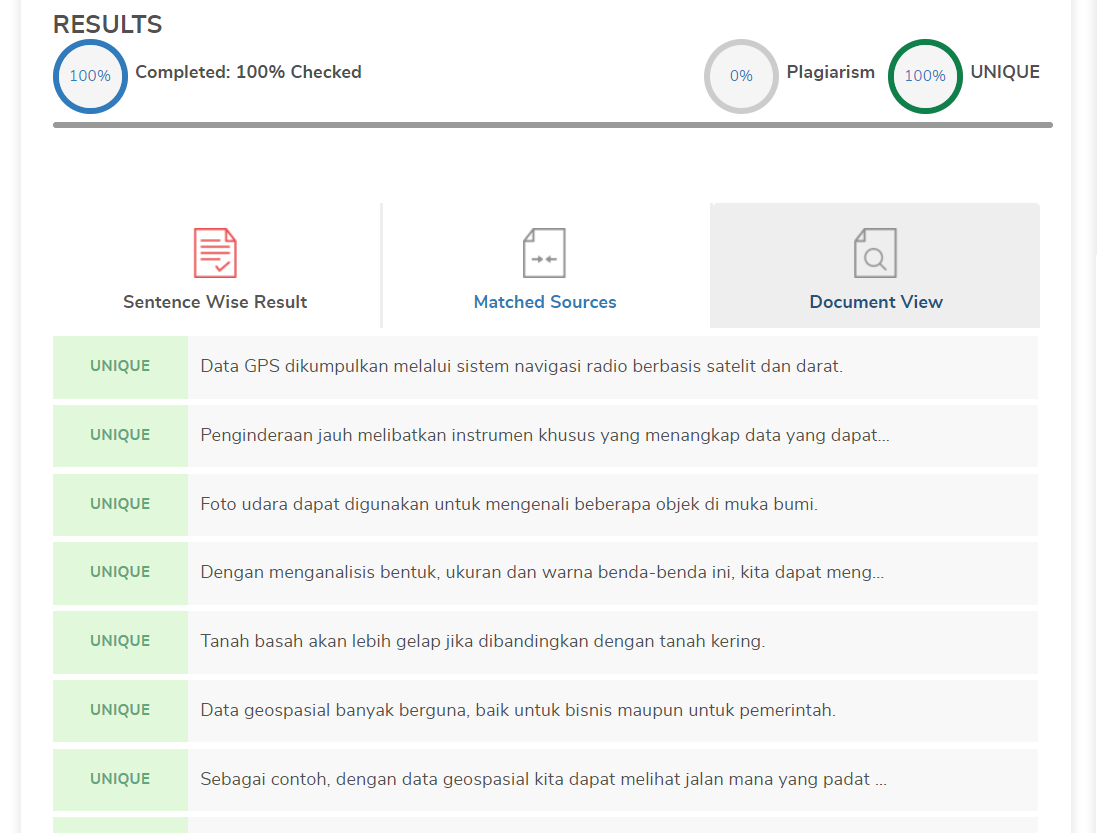
\includegraphics[width=4cm]{figures/1174026/1/4.png}
	\centering
	\caption{Bukti Tidak Melakukan Plagiat}
\end{figure}



%\section{Habib Abdul Rasyid (1174002)}
\subsection{Pengertian}
Sistem Informasi Geografis terdiri atas 3 kata. Yaitu Sistem, Informasi, dan Geografis.
\begin{itemize}
	\item SISTEM \break
Definisi sistem secara umum adalah unit yang terdiri dari komponen atau elemen yang saling berinteraksi, saling terkait, atau saling tergantung untuk membentuk keseluruhan yang kompleks.
	\item INFORMASI \break
Informasi adalah data yang telah diolah menjadi bentuk yang memiliki makna bagi penerimanya dan bisa dalam bentuk fakta, nilai-nilai bermanfaat. Pada bagian ini terdapat proses transformasi data menjadi informasi, yaitu proses input-output.
	\item GEOGRAFI \break
Geografi adalah studi tentang lokasi dan persamaan dan perbedaan variasi spasial dalam fenomena fisik dan manusia di permukaan bumi. Definisi lain dari geografi adalah studi tentang persamaan dan perbedaan dalam fenomena geologis dari perspektif regional dan lingkungan dalam konteks spasial.
	\item SISTEM INFORMASI \break
Pengertian Sistem informasi secara umum adalah sistem terintegrasi yang mampu memberikan informasi yang bermanfaat bagi penggunanya, memberikan informasi untuk mendukung operasi, manajemen dalam suatu organisasi. Sistem ini menggunakan perangkat keras dan lunak komputer, prosedur manual, model manajemen, dan basis data
	\item SISTEM INFORMASI GEOGRAFIS \break
Pengertian Sistem Informasi Geografis (SIG) secara umum adalah sistem informasi khusus yang digunakan untuk mengelola data yang memiliki informasi geospasial. GIS juga merupakan jenis perangkat lunak yang dapat digunakan untuk mengimpor, menyimpan, memanipulasi, menampilkan, dan mengeluarkan informasi geografis dan atributnya. GIS digunakan untuk memberikan nilai, dengan mengatur dan menampilkan data secara tepat, menggabungkannya dengan data lain, menganalisis data, dan menghasilkan data baru yang bermanfaat, pada gilirannya GIS dapat membantu untuk pengambilan keputusan. Sistem Informasi Geografis dibagi menjadi dua kelompok, yaitu sistem manual (analog), dan sistem otomatis (yang didasarkan pada komputer digital). Perbedaan paling mendasar terletak pada cara pengelolaannya.
\end{itemize}


\subsection{Sejarah}
Pada awal 1960-an perkembangan ilmu komputer berkembang pesat dan siap digunakan untuk bidang lain di luar militer. Ahli meteorologi, geologi dan geofisika mulai menggunakan komputer dalam membuat peta.
Pada tahun 1963 di Kanada, CGIS (Sistem Informasi Geografis Kanada) muncul, dan kemudian menjadi GIS pertama di dunia. Dua tahun kemudian di Amerika Serikat mengoperasikan sistem serupa yang disebut MIDAS yang digunakan untuk memproses data sumber daya alam.
Seiring dengan perkembangan teknologi, GIS juga telah berubah menjadi lebih baik. Berikut ini adalah sejarah perkembangan SIG dari waktu ke waktu:
\begin{itemize}
	\item35.000 tahun lalu, di dinding gua Lascaux, Prancis, pemburu Cro-Magnon menggambar hewan mangsa mereka, serta garis yang diyakini sebagai rute migrasi hewan-hewan. Catatan awal ini sejalan dengan dua elemen struktural dalam sistem informasi geografis modern saat ini, arsip grafik yang terhubung ke database atribut.
	\item Pada 1700-an, teknik survei modern untuk pemetaan topografi diterapkan, termasuk versi awal pemetaan tematik, misalnya untuk data ilmiah atau sensus.
	\item Awal abad ke-20 menyaksikan perkembangan "foto litograf" di mana peta dipisahkan menjadi beberapa lapisan. Perkembangan perangkat keras komputer yang didorong oleh penelitian senjata nuklir membawa aplikasi pemetaan ke multifungsi pada awal 1960-an.
	\item 1967 adalah awal dari pengembangan GIS yang dapat diimplementasikan di Ottawa, Ontario oleh Departemen Energi, Tambang dan Sumber Daya. Dikembangkan oleh Roger Tomlinson, yang kemudian disebut CGIS (GIS Kanada - GIS Kanada), digunakan untuk menyimpan, menganalisis, dan memproses data yang dikumpulkan untuk Inventarisasi Tanah Kanada (CLI - inventaris tanah Kanada) - sebuah inisiatif untuk mengetahui kemampuan lahan di pedesaan Kanada dengan peta. berbagai informasi tentang tanah, pertanian, pariwisata, liar, unggas dan penggunaan lahan pada skala 1: 250000. Klasifikasi faktor peringkat juga diterapkan untuk analisis.
	\item GIS dengan gvSIG.CGIS adalah sistem pertama di dunia dan hasil dari aplikasi pemetaan yang disempurnakan yang memiliki kemampuan untuk melapisi, menghitung, mendigitalkan / memindai, mendukung sistem koordinat nasional yang memanjang melintasi benua Amerika, memasukkan garis sebagai busur dengan atribut topologi dan toko dan informasi lokasi dalam file terpisah. Pengembang, seorang ahli geografi bernama Roger Tomlinson, kemudian dipanggil "Mr. GIS".
	\item CGIS bertahan hingga tahun 1970-an dan membutuhkan waktu lama untuk membaik setelah pengembangan awal, dan tidak dapat bersaing dengan aplikasi pemetaan komersial yang dirilis oleh vendor seperti Intergraph. Pengembangan perangkat keras komputer mikro mendorong vendor lain seperti ESRI dan CARIS untuk membuat banyak fitur GIS, menggabungkan pendekatan generasi pertama dengan pemisahan informasi spasial dan atribut, dengan pendekatan generasi kedua pada organisasi data atribut ke dalam struktur basis data. Pengembangan industri pada 1980-an dan 1990-an semakin memacu pertumbuhan GIS pada workstation UNIX dan komputer pribadi. Pada akhir abad ke-20, pertumbuhan yang cepat di berbagai sistem dikonsolidasikan dan distandarisasi ke dalam platform yang lebih sedikit, dan pengguna mulai mengekspor tampilan data GIS melalui internet, yang membutuhkan standar pada format dan transfer data.
\end{itemize}



\subsection{Koordinasi}
Untuk menggambarkan permukaan bumi yang berbentuk seperti bola menjadi bentuk peta, kita membutuhkan persamaan matematika yang dapat membantu mengubah citra permukaan bumi. Persamaan ini disebut sistem koordinat. Koordinat adalah karakteristik utama SIG karena sistem koordinat ini dapat menunjukkan referensi geografis pada data SIG. Dapat dikatakan bahwa sistem koordinat adalah pendekatan dalam mendefinisikan posisi data SIG di permukaan bumi.
Dalam sistem koordinat, posisi benda di permukaan bumi ditentukan oleh garis lintang dan bujur. Latitude adalah garis horizontal yang mengukur sudut antara titik dan khatulistiwa (khatulistiwa). Sedangkan garis bujur adalah garis vertikal yang mengukur sudut suatu titik dengan titik nol bumi, yaitu Greenwich Meridian, London
Lintang dibagi menjadi 2, yaitu lintang utara dan selatan dan bujur dibagi menjadi bujur timur dan bujur barat. Sumbu x sebagai garis lintang dan sumbu y sebagai garis bujur dalam koordinat Cartesius.

\subsection{Geospasial}
Data geospasial adalah data tentang aspek fisik dan administrasi dari suatu objek geografis. Aspek fisik yang dimaksud meliputi bentuk-bentuk antropogenik dan alami baik di permukaan maupun di bawah permukaan bumi. Bentuk antropogenik mengandung fenomena budaya seperti jalan, rel kereta api, bangunan, jembatan, dan sebagainya. Tentu saja alam adalah sungai, danau, pantai, dataran tinggi, dan sebagainya. Sedangkan aspek administratif adalah batas distribusi atau sosial-budaya yang dibuat oleh suatu organisasi atau lembaga dengan tujuan mengatur dan menggunakan sumber daya alam. Termasuk dalam aspek perbatasan negara, pembagian wilayah administratif, zona, kode pos, batas kepemilikan tanah, dan sebagainya.
Secara umum ada dua metode untuk menampilkan fitur geografis ke GIS atau Sistem Informasi Geospasial. Pertama, struktur data vektor (struktur data vektor) terdiri dari deskripsi titik geografis, dalam bentuk titik, garis, atau poligon. Model grafik vektor ini menampilkan fitur geografis terpisah seperti batas administratif, jalan, bangunan, dan sungai. Objek grafis biasanya dikaitkan dengan informasi yang berisi penjelasan tentang atribut objek, dan informasi ini dapat disimpan dalam spreadsheet atau file database yang terpisah. Kedua, struktur data raster terdiri dari serangkaian sel atau piksel yang biasanya digunakan untuk menggambarkan data gambar sebagai data kontinu. Dalam struktur data seperti itu, ada unsur resolusi sebagai ukuran dimensi fitur geografis yang direpresentasikan dalam bentuk piksel. Biasanya data raster ini digunakan untuk citra satelit, ortografi digital, model elevasi digital, peta digital.

\subsection{Link}
\href{https://youtu.be/zhZPF4EKivU}{https://youtu.be/zhZPF4EKivU}

\subsection{Plagiarism}
\begin{figure}[H]
	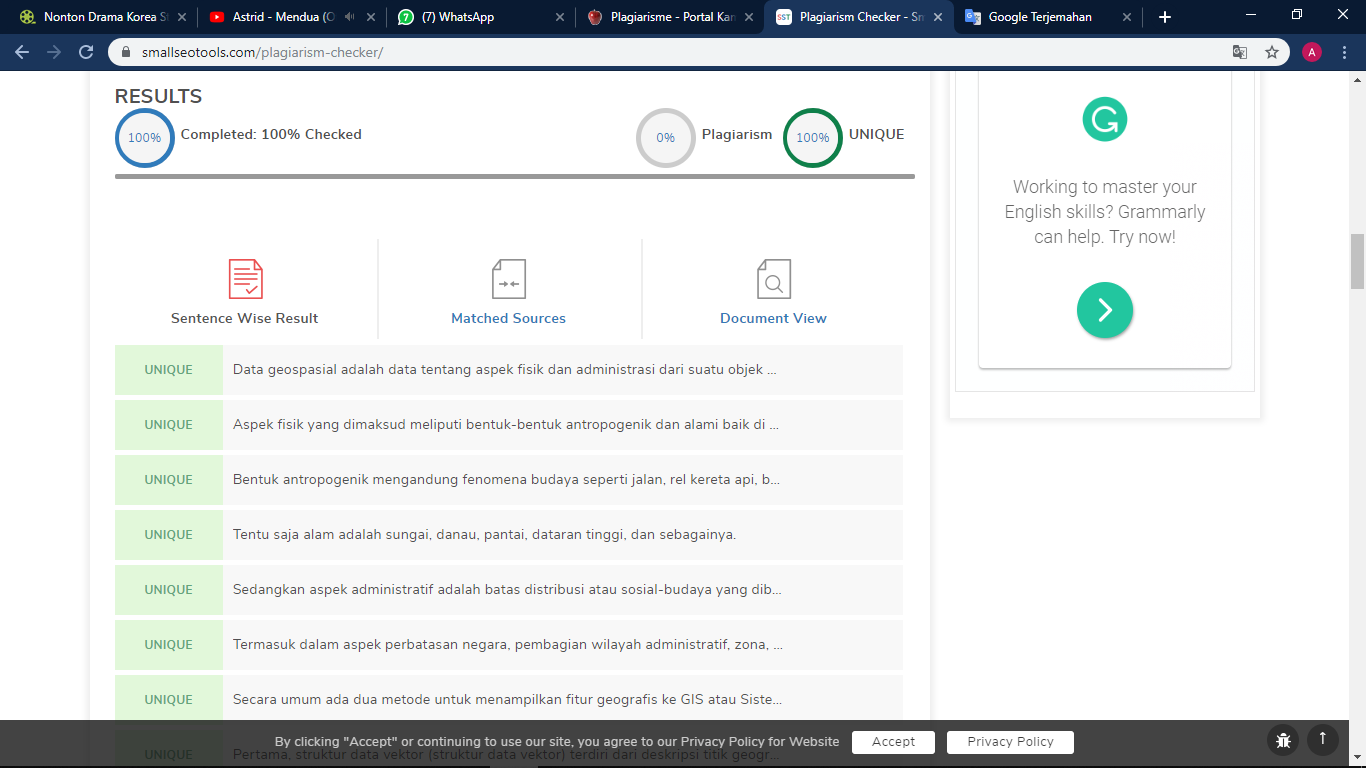
\includegraphics[width=4cm]{figures/1174002/SSGIS.png}
	\centering
	\caption{Plagiarism 1174002}
\end{figure}

%\section{Harun Ar - Rasyid(1174027)}
\subsection{Pengertian}
Geografi adalah ilmu pengetahuan yang mengambarkan segala sesuatu yang ada di permukaan bumi. \hfill\break
Geografi juga selain mempelajari bagian permukaan bumi, tapi juga mempelajari seluruh bagian bumi mulai darti struktur bumi,jenis batuan yang menyusun bumi serta atmosfer yang melindungi bumi. \hfill\break
Segala aktifitas yang terjadi di bumi merupakan bagian dari ilmu Geografi.\hfill\break
\subsection{Sejarah}
Sejarah geografi dimulai sejak manusia mulai berinteraksi dengan lingkunganya, hal ini juga merupakan awal mula dari berkembangnya ilmu pengetahuan tentang geografi.\hfill\break
Pada awalnya geografi hanya membahas atau mendekripsikan gambaran umum tentang fakta-fakta yang menjelaskan keadaan di muka bumi. Pada abad ke-18 yaitu masa geografi klasik, ilmu geografi hanya sebatas menjelaskan dan mengumpulkan informasi tentang lingkungan geografi saja, misalnya: keadaan politik, industri, iklim terutama di kota-kota besar.\hfill\break
Sejarah geografi terus berjalan dan berkembang. Tepatnya, diabad ke-19 geografi mengalami perkembangan dari segi keilmuannya. Dari yang semula hanya mendeskripsikan saja kemudian berkembang menjadi lebih spesifik yaitu dengan menjelaskan lingkungan geografi secara sistematis.\hfill\break
Pada pertengahan abad ke-19, keilmuan dalam geografi sudah membahas sampai ketingkat membandingkan keadaan, data geografis dan karakteristik antara wilayah yang satu dengan wilayah yang lain di muka bumi. Hal ini kita kenal sebagai “Comparative Geography”.\hfill\break
Perkembangan keilmuwan geografi semakin pesat pasca terjadinya perang dunia ke-II. Yang semula dikembangkan oleh imuwan Amerika dan Inggris yang dikenal sebagai “Comparative Geography” kemudian berkembang menjadi “Global Geography” dimana objek kajiannya semakin luas yaitu meliputi seluruh dunia. Era inilah yang dinamakan sebagai “era geografi modern”.\hfill\break
Dari pembahasan di atas, kita sudah mengetahui kapan sejarah geografi itu dimulai yaitu sejak adanya interaksi antara manusia dengan lingkungannya. Bila seperti itu, maka hakekatnya sejak Nabi Adam as turun ke bumi sebetulnya geografi sudah ada.\hfill\break
Akan tetapi penggalian geografi secara keilmuan sendiri baru dilakukan pertama kali oleh orang-orang Yunani. Dimana pada perkembangan awalnya dilatarbelakangi oleh suatu upaya masyarakat Yunani untuk melepaskan diri dari alam pikiran dan kepercayaan. Dimana kepercayaan tersebut meyakini bahwa dewa-dewa ikut turut campur dalam segala bentuk kejadian di bumi.\hfill\break
Istilah geografi sebenarnya baru digunakan pada tahun 1972 sedangkan sebelumnya lebih menggunakan istilah “ilmu bumi”. Istilah ini pertama kali diperkenalkan oleh seorang ahli filsafat dan astronomi yang bernama Eratosthenes pada 276 194 sebelum masehi.Kemudian, Claudius Ptoleumaeus melakukan peletakan dasar-dasar keilmuan geografi.\hfill\break
Sejarah perkembangan geografi terus berlanjut. Immanuel Kant mengembangkan geografi modern kemudian Karl Ritter juga mengembangkan geografi sosial.\hfill\break
Selain itu ada tokoh-tokoh lain yang ikut andil dalam mengembangkan geografi yaitu Alexander von Humbolt sebagai peletak dasar geografi fisika modern dan sebagainya.\hfill\break
\subsection{Koordinat}
Koordinat didapatkan dari hasil perpotongan antara garis latitude (Y) / lintang dan garis longitude(X) / garis bujur sehingga bisa menunjukan suatu lokasi pada suatu daerah. \hfill\break 
Umumnya koordinat dibedakan menajadi koordinat Geografi dan Universal Transver Mercator(UTM). Pada koordinat geografi dibedakan menajadi 3 yaitu : \hfill\break
\begin{itemize}
	\item Degree, Decimal(DD, DDDD) contoh S 4.56734 E 102.67235
	\item Degree,Minute(DD MM,MMMM) contoh S 4 42,5423’ E 105 34,6445’
	\item Degree, Minute, Second(DD MM SS,SS) contoh : S 4 43’ 45,22 E 103 33’ 33,25
\end{itemize}
\hfill\break
\begin{figure}[H]
	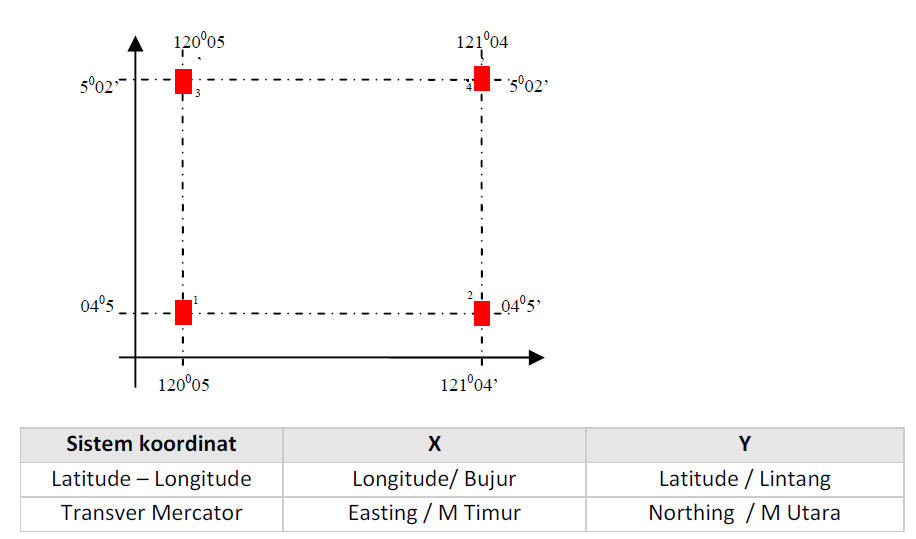
\includegraphics[width=4cm]{figures/1174027/1_1174027_koordinat.jpg}
	\centering
	\caption{Contoh Koordinat}
\end{figure}
Pada system koordinat UTM biasanya terdapat pembagian waktu berdasarkan zonasinya. \hfill\break
\begin{figure}[H]
	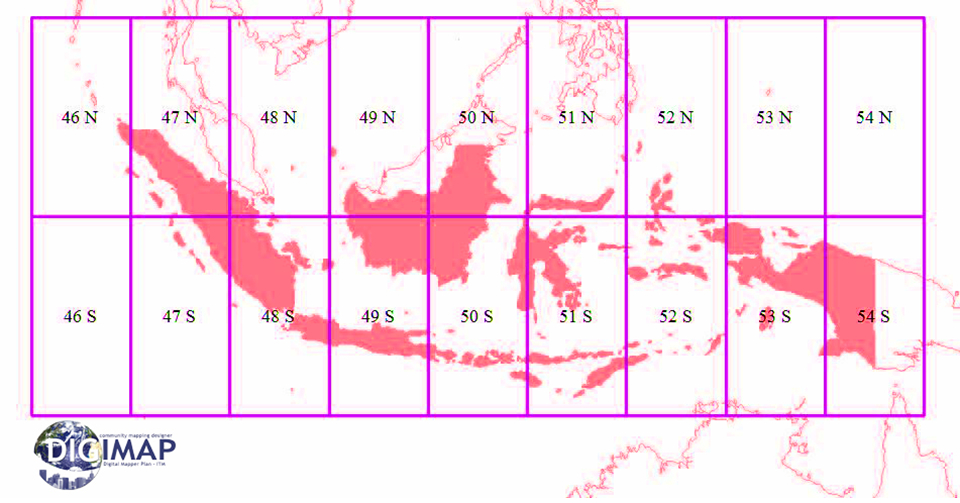
\includegraphics[width=4cm]{figures/1174027/1_1174027_UTM.jpg}
	\centering
	\caption{Contoh Koordinat UTM}
\end{figure}

\subsection{Data Geospasial}
Data geospasial merupakan pengambaran lokasi geografis,dimensi atau ukuran / karakteristik objek alam atau buatan manusia yang berada di bawah atau di atas permukaan bumi, data geospasial biasanya di singkat menjadi DG.
\hfill\break
Data Geospasial dibagi menjadi 2 yaitu :
\begin{itemize}
	\item Vektor
	Vektor merupakan salah jenis gambar yang dapat dibuat menggunakan aplikasi corel / adobe illustrator / aplikasi vektor lainnya. \hfill\break 
	Vektor itu sering digunakan untuk membuat gambar animasi dan vektor juga digunakan oleh goole maps.
	\item Roshen
	Roshen merupakan gambar yang di ambil dari satelit di luar angkasa, gambar ini biasanya bertipe jpg, dan pembaharuan data gambar ini berlangsung lama karena proses nya yang memakan waktu cukup banyak, jenis data ini digunakan oleh google earth.
\end{itemize}
\subsection{Link}
\begin{itemize}
	\item \href{https://youtu.be/mhk9PhmNLvk}{Pengertian GIS}
	\item \href{https://youtu.be/7K0x-oQncy4}{Sejarah GIS}
	\item \href{https://youtu.be/QE8uvqNqbo4}{Koordinat}
	\item \href{https://youtu.be/CXYenLiAS8U}{Data Geospasial}
\end{itemize}
\subsection{Plagiarism}
\begin{figure}[H]
	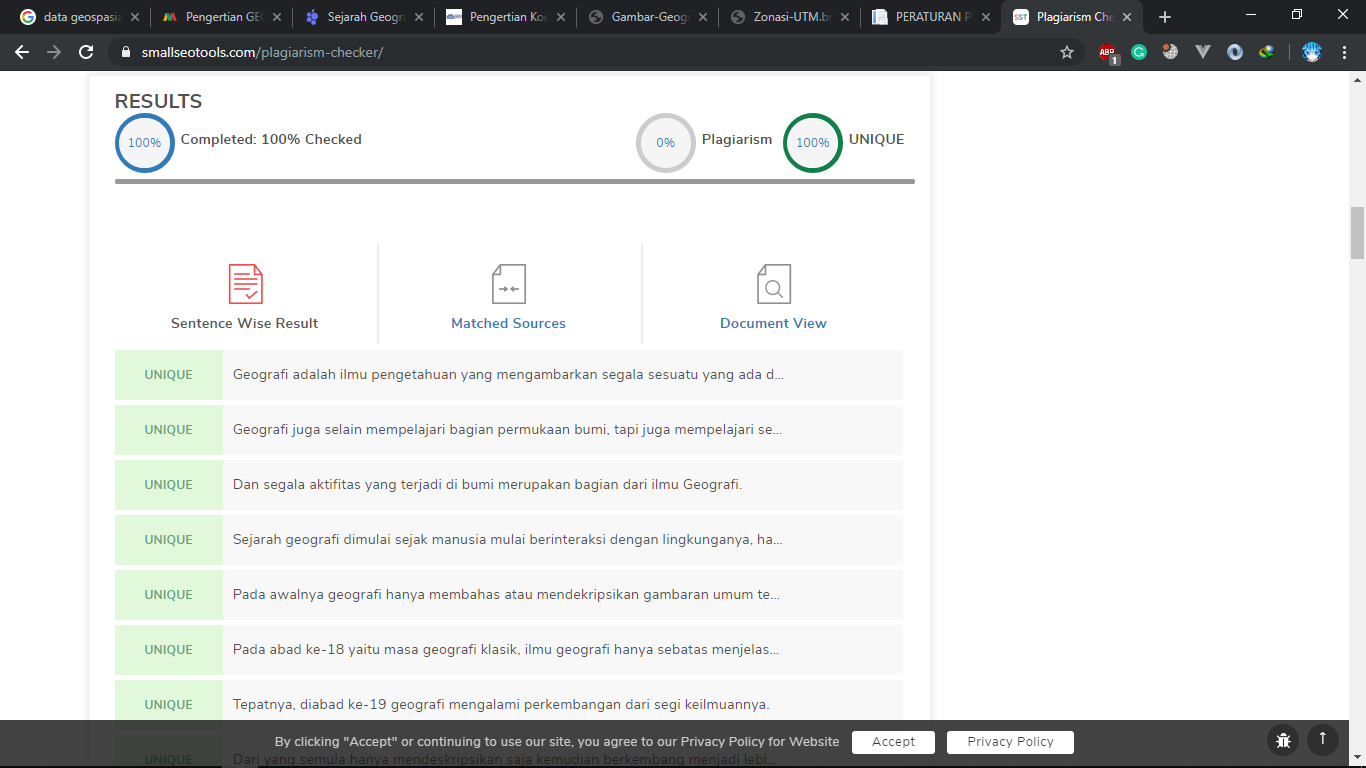
\includegraphics[width=4cm]{figures/1174027/1_1174027_placek.png}
	\centering
	\caption{Bukti Tidak Melakukan Plagiat}
\end{figure}
%\section{Kadek Diva Krishna Murti (1174006)}
\subsection{Pengertian}
\begin{figure}[H]
	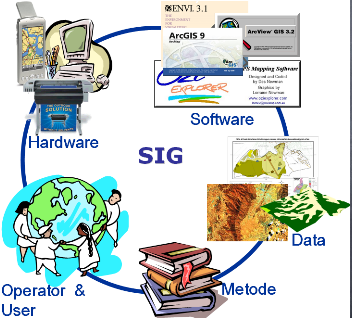
\includegraphics[width=4cm]{figures/1174006/1174006sig1.png}
	\centering
	\caption{Sistem Informasi Geografis.}
\end{figure}
Sistem Informasi Geografis merupakan sebuah runtutan kegiatan yang dilakukan untuk mendapatkan sebuah gambaran mengenai keadaaan ruang muka bumi atau informasi mengenai ruang muka bumi yang dibutuhkan untuk menjawab atau menyelesaikan suatu permasalahan yang ada pada ruang muka bumi yang bersangkutan. Runtutan kegiatan tersebut seperti pengumpulan, penataan, pengolahan, penganalisisan dan penyajian data-data atau fakta-fakta yang terdapat pada ruang muka bumi tertentu. Data atau fakta tersebut disebut sebagai data atau fakta geografis atau data atau fakta spatial. Hasil analisisnya disebut Informasi geografis atau Informasi spatial. Jadi Sistem Informasi Geografis merupakan runtutan kegiatan pengumpulan, penataan, pengolahan dan penganalisisan data atau fakta spatial sehingga diperoleh informasi spasial untuk dapat menjawab atau menyelesaikan suatu permasalahan pada ruang muka bumi tertentu.
\subsection{Sejarah}
\begin{figure}[H]
	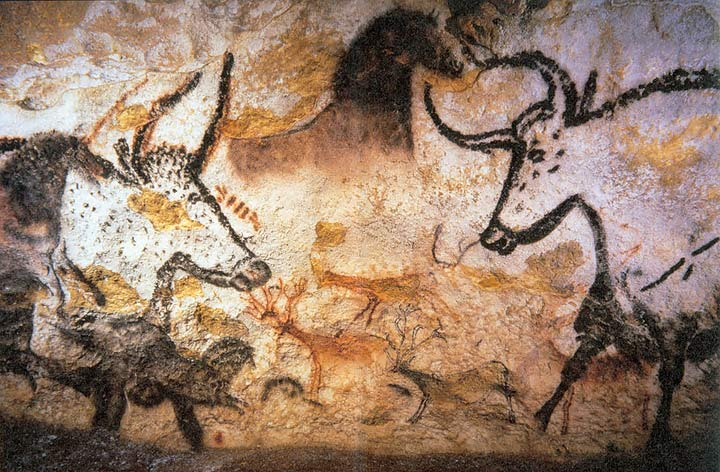
\includegraphics[width=4cm]{figures/1174006/1174006gua1.jpg}
	\centering
	\caption{Gua Lascaux.}
\end{figure}
Pada 35000 tahun yang lalu, di sebuah dinding tepatnya di gua Lascaux, Perancis, para pemburu Cro-Magnon menggambarkan hewan-hewan mangsa mereka. Mereka juga menggambarkan garis-garis yang dipercaya sebagai rute dari migrasi hewan-hewan mangsa mereka tersebut. Catatan awal tersebut sejalan dengan dua elemen struktur pada sistem informasi geografis modern saat ini, arsip grafis yang terhubung ke database atribut. 
Lalu pada tahun 1700-an teknik survei modern untuk pemetaan topografis diterapkan, termasuk versi awal pemetaan tematis, contohnya untuk keilmuan atau data sensus. 
Kemudian pada awal abad ke-20 memperlihatkan pengembangan "litografi foto" dimana peta dipisahkan menjadi beberapa lapisan (layer). Perkembangan perangkat keras komputer yang dipacu oleh penelitian senjata nuklir membawa aplikasi pemetaan menjadi multifungsi pada awal tahun 1960-an. 
Setelah itu, pada tahun 1967 menjadi awal pengembangan sistem informasi geografis yang bisa diterapkan di Ottawa, Ontario oleh Departemen Energi, Pertambangan dan Sumber Daya. Sistem ini dikembangkan oleh Roger Tomlinson, yang kemudian disebut CGIS (Canadian GIS - SIG Kanada) yang digunakan untuk menyimpan, menganalisis dan mengolah data-data yang sebelumnya telah dikumpulkan untuk kepentingan Inventarisasi Tanah di Kanada (CLI - Canadian land Inventory) - dimana ini merupakan sebuah inisiatif untuk mengetahui kemampuan dari suatu lahan yang ada di wilayah pedesaan Kanada dengan cara memetakaan berbagai informasi mengenai tanah, pertanian, pariwisata, alam bebas, unggas dan penggunaan tanah pada skala 1:250000. Faktor pemeringkatan klasifikasi juga diterapkan untuk keperluan analisis.
\begin{figure}[H]
	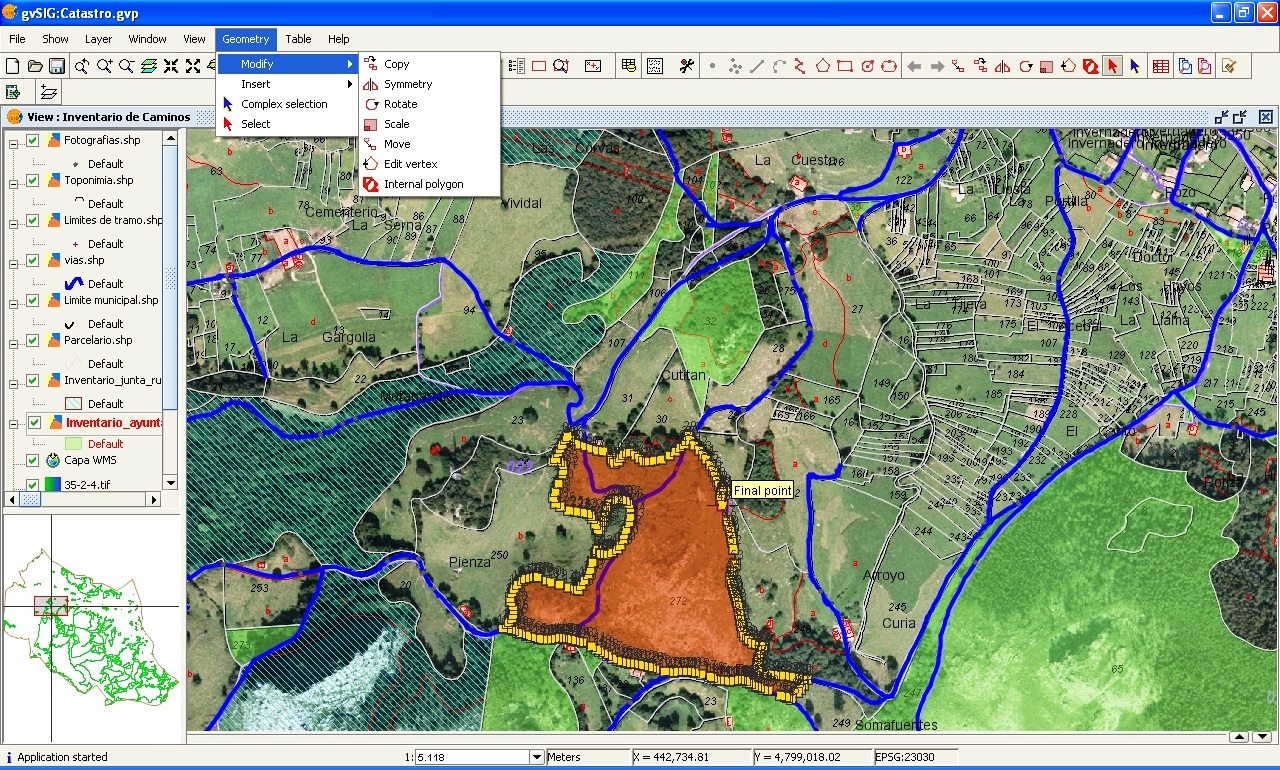
\includegraphics[width=4cm]{figures/1174006/1174006sigapp1.jpg}
	\centering
	\caption{Aplikasi SIG.}
\end{figure}
\subsection{Koordinat}
Koordinat digunakan untuk menunjukkan suatu titik di bumi berdasarkan garis lintang dan garis bujur. Koordinat dibagi menjadi dua bagian irisan yaitu irisan melintang yang disebut dengan garis lintang mulai dari khatulistiwa, membesar ke arah kutub(utara mupun selatan) sedangkanyang lain membujur mulai dari garis Greenwhich membesar ke arah barat dan timur. Satuan skala pada koordinat dibagi menjadi derajat lintang 0\textdegree sampai 90\textdegree dan bujur 0\textdegree sampai 180\textdegree.
Informasi sebuah lokasi didasarkan pada sistem koordinat, yang mencakup datum dan proyeksi peta. Datum adalah kumpulan parameter dan titik kontrol yanghubungan geometriknya diketahui, baik melalui pengukuranatau penghitungan. Sedangkan sistem proyeksi peta adalah sistem yang dirancang untuk merepresentasikan permukaan dari suatu bidang lengkung atau spheroid (misalnya bumi) pada suatu bidang datar. Proses representasi ini menyebabkan distorsi yang perlu diperhitungkan untuk memperoleh ketelitian beberapa macam properti, seperti jarak, sudut, atau luasan.
\begin{figure}[H]
	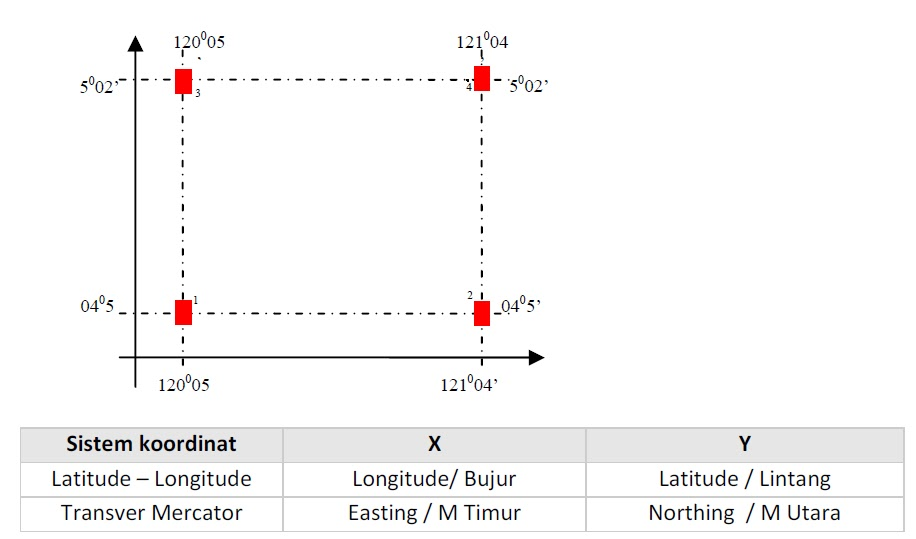
\includegraphics[width=4cm]{figures/1174006/1174006koordinat1.jpg}
	\centering
	\caption{Sistem Koordinat.}
\end{figure}
\subsection{Data Geospasial}
\subsubsection{Data Vektor}
Data vektor adalah data yang direkam dalam bentuk koordinat titik yang menampilkan, menempatkan, dan menyimpan data spasial dengan menggunakan titik, garis atau area (polygon).
\begin{figure}[H]
	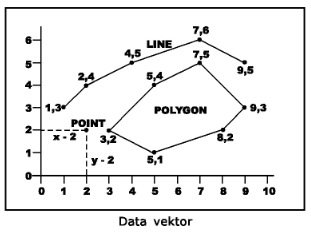
\includegraphics[width=4cm]{figures/1174006/1174006vektor1.png}
	\centering
	\caption{Data Vektor.}
\end{figure}
Ada tipe-tipe data vector yang bisa digunakan untuk menampilkan informasi pada peta. 
\begin{enumerate}
	\item Titik bisa digunakan sebagai lokasi sebuah kota atau posisi tower radio. 
	\item Garis bisa digunakan untuk menunjukkan route suatu perjalanan atau menggambarkan boundary.
	\item Poligon bisa digunakan untuk menggambarkan sebuah danau atau sebuah Negara pada peta dunia.
\end{enumerate}

\subsubsection{Data Raster}
Data raster adalah data yang disimpan dalam bentuk grid atau petak sehingga terbentuk suatu ruang yang teratur dalam bentuk pixel. 
Foto digital seperti areal fotografi atau satelit merupakan bagian dari data raster pada peta.
\begin{figure}[H]
	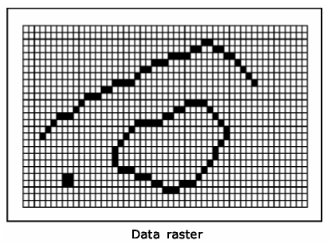
\includegraphics[width=4cm]{figures/1174006/1174006raster1.png}
	\centering
	\caption{Data Raster.}
\end{figure}
Data raster dihasilkan dari sistem penginderaan jauh dan sangat baik untuk merepresentasikan batas-batas yang berubah secara gradual seperti jenis tanah, kelembaban tanah, suhu, dan lain-lain.
Obyek geografis pada data rastel direpresentasikan sebagai struktur sel grid yang disebut sebagai pixel.
Resolusi tergantung pada ukuran pixelnya, semakin kecil ukuran permukaan bumi yang direpresentasikan oleh sel, semakin tinggi resolusinya. Dengan kata lain, resolusi pixel menggambarkan ukuran sebenarnya dipermukaan bumi yang diwakili oleh setiap pixel pada citra.

\subsubsection{Perbedaan Data Vektor dan Data Rastel}
Data vektor relatif lebih ekonomis dalam hal ukuran file dan presisi dalam lokasi. Tetapi sangat sulit untuk digunakan dalam komputasi matematik. Sebaliknya data raster biasanya membutuhkan ruang penyimpanan file yang lebih besar dan presisi lokasinya lebih rendah tetapi lebih mudah digunakan secara matematis.

\subsection{Link}
\href{https://youtu.be/2BjDss7m9SQ}{https://youtu.be/2BjDss7m9SQ}

\subsection{Plagiarism}
\begin{figure}[H]
	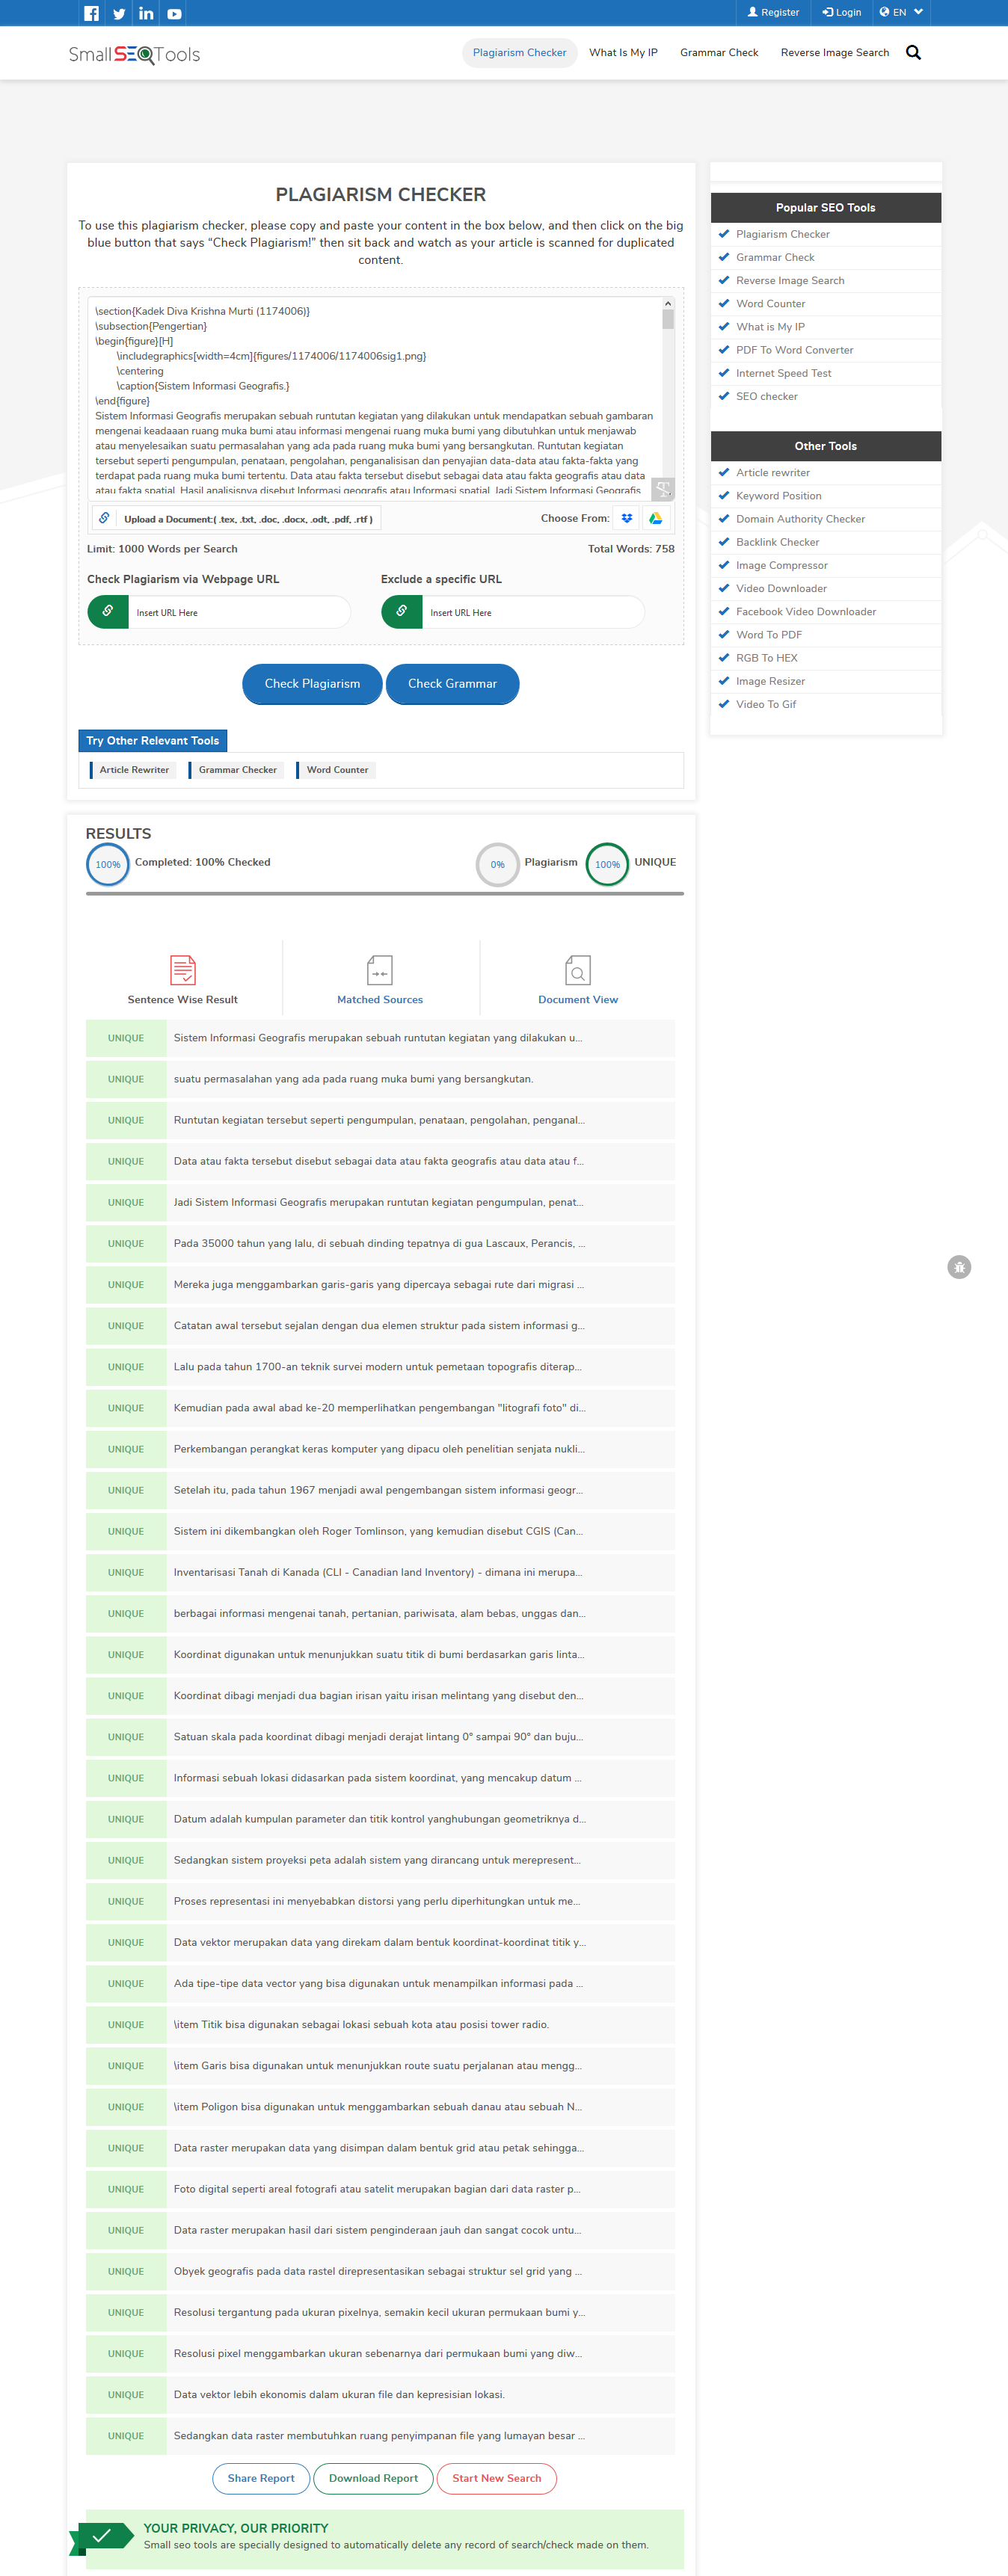
\includegraphics[width=4cm]{figures/1174006/1174006plagiarism1.png}
	\centering
	\caption{Plagiarism 1174006.}
\end{figure}

%\section{Muhammad Dzihan Al-Banna (1174095)}
\subsection{Pengertian}
GIS atau juga bias disebut Sistem Informasi Geografis adalah sistem informasi yang mengelola data yang memiliki informasi spasial yang bereferensi ke ruangan. Sistem informasi geografis adalah sistem komputer yang mempunyai kemampuan untuk membangun, menyimpan, mengelola dan menampilkan informasi berpatokan pada geografis, misalnya data diidentifikasi menurut lokasinya dalam sebuah database.SIG dapat digunakan perencana untuk membantu menghitung waktu tanggap darurat saat terjadi bencana alam secara cepat dan lain sebagainya.
\subsection{Sejarah}
3500 tahun lalu pemburu Cro-Magnon menggambar hewan mangsa mereka, dan juga garis yang dipercaya sebagai rute migrasi hewan-hewan tersebut. Catatan awal ini sejalan dengan dua elemen struktur pada sistem informasi geografis modern sekarang ini, arsip grafis yang terhubung ke database atribut.
Pada tahun 1700 an teknik survey modern untuk pemetaan topografis diterapkan, termasuk juga versi awal pemetaan tematis, misalnya untuk keilmuan atau sensus.
Kemudian pada awal abad ke 20 terdapat pengembangan litografi foto dimana peta dipisahkan menjadi beberapa lapisan . Perkembangan perangkat keras komputer yang dipacu oleh penelitian senjata nuklir membawa aplikasi pemetaan menjadi multifungsi pada awal tahun 1960 an.
Tahun 1967 Departemen Energi, Pertambangan dan Sumber Daya Dikembangkan oleh Roger Tomlinson yang disebut CGIS.
GIS dengan gvSIG.
CGIS merupakan sistem hasil dari perbaikan aplikasi pemetaan yang memiliki kemampuan timpang susun, penghitungan, pemindaian, mendukung sistem koordinat national yang membentang di atas benua Amerika. ESRI, CARIS,  MapInfo berhasil membuat banyak fitur SIG. Pada tahun 1980 an dan 1990 an perkembangan industri memacu lagi pertumbuhan SIG pada workstation UNIX dan komputer pribadi. di berbagai sistem dikonsolidasikan dan distandarisasikan menjadi platform lebih sedikit, dan para pengguna mulai mengekspor menampilkan data SIG lewat internet Pada akhir abad ke-20, yang membutuhkan standar pada format data dan transfer.

\subsection{Koordinat}
Koordinat adalah suatu titik yang didapatkan dari hasil perpotongan dari garis lintang dengan garis bujur sehingga akan menunjukan lokasi pada suatu daerah. Umumnya koordinat dibedakan menjadi koordinat Geographic dan Universal Transver Mercator.
Pada Sistem Koordinat UTM biasanya terdapat pembagian waktu berdasarkan zonasinya, di Indonesia sendiri terdapat 16 pembagian zonasi waktu, pada Gambar 2 menjelaskan pembagian zonasi waktu dimana terdapat garis yang memisahkan dari garis khatulistiwa. Untuk Daerah yang berada di atas garis khatulistiwa akan mempunyai Kode N sedangkan yang berada dibawah khatulistiwa akan mempunyai kode S.

\begin{figure}[H]
	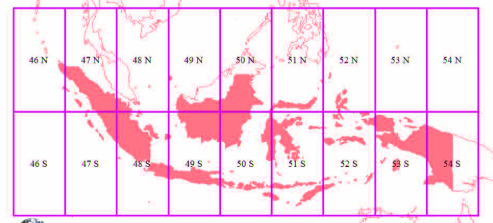
\includegraphics[width=4cm]{figures/1174095/dzihan.png}
	\centering
	\caption{Pembagian Zona Waktu}
\end{figure}

\subsection{Data Geospasial}
Data spasial adalah data yang memiliki referensi ruang kebumian (georeference) di mana berbagai data atribut terletak dalam berbagai unit spasial. data spasial  sangat penting untuk perencanaan pembangunan dan pengelolaan sumber daya alam.
Data spasial terbagi menjadi dua yaitu :
Data vektor adalah data yang direpresentasikan sebagai suatu mosaik berupa garis, polygon, titik/point, dan nodes. Salah satu keuntungan dari format data vektor adalah akurasi dalam merepresentasikan fitur titik, batasan dan garis lurus.

Data Vektor berguna untuk analisa yang membutuhkan ketepatan posisi, misalnya pada basis data batas-batas kadaster. Contoh penggunaan lainnya adalah untuk mendefinisikan hubungan spasial dari beberapa fitur. vektor memiliki kekurangan yaitu ketidakmampuannya dalam mengakomodasi perubahan gradual.
	Data Raster
Data raster adalah data hasil dari penginderaan secara jauh. Data Raster sering disebut juga dengan sel grid. Dalam data raster obyek geografis direpresentasikan sebagai struktur sel grid yang disebut dengan pixel (picture element). Resolusi data raster tergantung pada ukuran pixel-nya .resolusi pixel menggambarkan ukuran sebenarnya di permukaan bumi yang diwakili oleh setiap pixel pada citra
\subsection{Link}
\href{https://youtu.be/KLmO0eBCJAQ}{Lihat Videonya disini}
\subsection{Plagiarism}
\begin{figure}[H]
	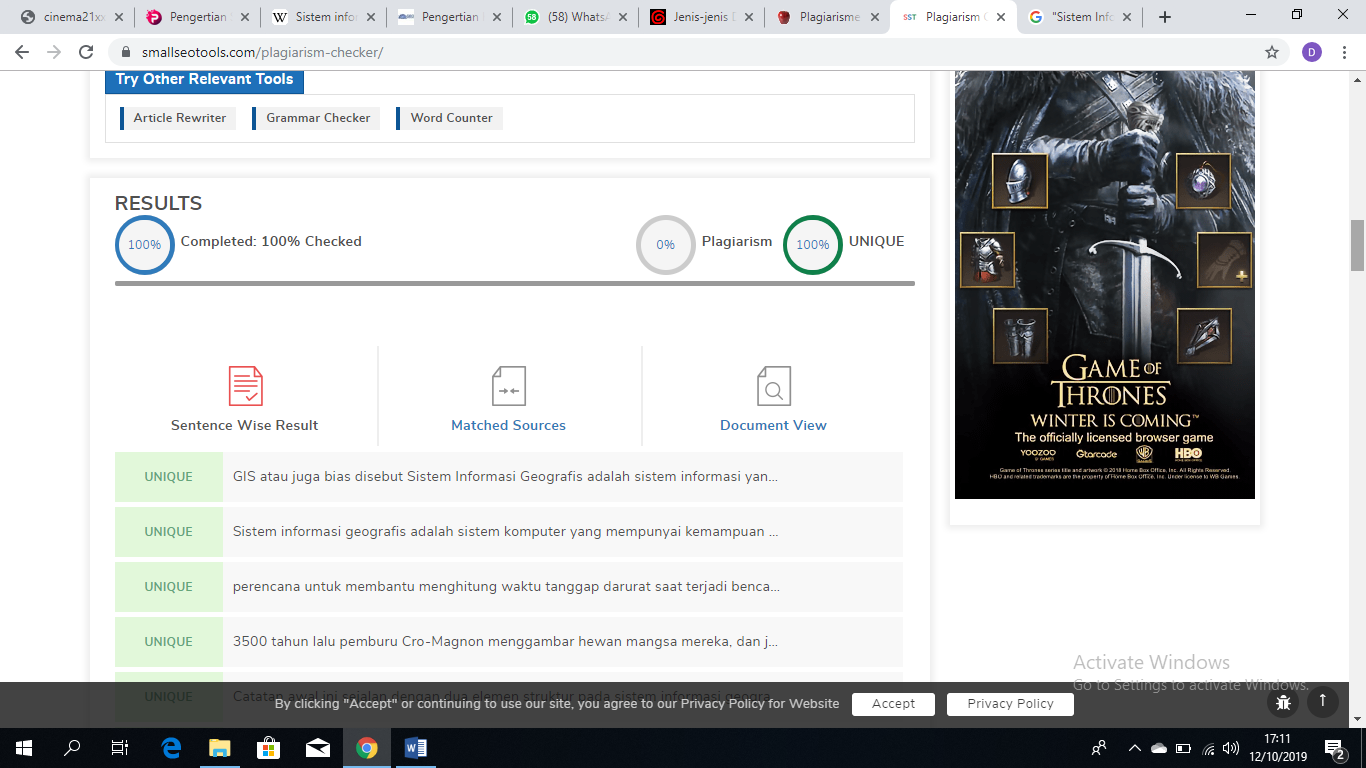
\includegraphics[width=4cm]{figures/1174095/plag.png}
	\centering
	\caption{Plagiarisme}
\end{figure}

%\section{Muhammad Fahmi (1174021)}

\subsection{Pengertian}
Pengertian geografi adalah bidang ilmu yang secara khusus mempelajari lokasi dan persamaan serta perbedaan spasial dari fenomena fisik, dan manusia di permukaan bumi. \hfill\break
Pendapat lain mengatakan definisi geografi adalah studi tentang karakteristik fisik bumi dan atmosfernya, dan aktivitas manusia yang mempengaruhi dan dipengaruhi, termasuk distribusi populasi dan sumber daya, penggunaan lahan, dan industri. \hfill\break
Secara etimologis, istilah "geografi" berasal dari bahasa Yunani, yaitu kata "geo" yang berarti bumi, dan "graphien" yang berarti pencitraan. Sehingga geografi dapat didefinisikan sebagai ilmu yang menggambarkan segala sesuatu yang ada di permukaan bumi.\hfill\break

Agar lebih memahami apa itu geografi, maka kita dapat merujuk pada pendapat beberapa ahli berikut ini: \hfill\break
\begin{itemize}
	\item Claudius Ptolomaeus
Menurut pendapat Claudius Ptolomaeus, definisi geografi adalah presentasi melalui peta sebagian dan seluruh permukaan bumi.
	\item Preston E. James
Menurut pendapat Preston E. James, definisi geografi adalah ibu dari semua ilmu, ini karena bidang sains selalu berawal dari keadaan bumi yang kemudian beralih ke studi masing-masing ilmu.
	\item Frank Debenham
Frank Debenham mengatakan bahwa pengertian geografi adalah ilmu yang bertugas membuat interpretasi tentang distribusi fakta, menemukan hubungan antara kehidupan manusia dan lingkungan fisik, dan menjelaskan kekuatan interaksi antara manusia dan alam.
	\item Mustofa Bisri
Menurut Mustofa Bisri, definisi geografi adalah ilmu yang menggambarkan permukaan bumi, iklim, populasi, flora dan fauna, serta hasil yang ditemukan di bumi. 
\end{itemize} \hfill\break

\begin{figure}[H]
	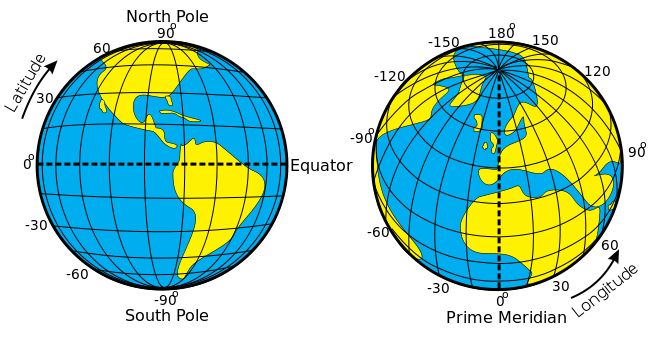
\includegraphics[width=4cm]{figures/1174021/1.png}
	\centering
	\caption{Sistem Informasi Geografis.}
\end{figure}


\subsection{Sejarah}
Sejarah geografi dimulai dengan interaksi antara manusia dan lingkungannya. Ini adalah awal dari perkembangan geografi.
Awalnya, geografi hanya dibahas atau dijelaskan dalam deskripsi umum fakta yang dijelaskan kondisi di bumi. Pada abad ke-18, yaitu era geografi klasik, geografi terbatas pada menjelaskan dan mengumpulkan informasi tentang lingkungan geografis, misalnya: kondisi politik, industri, iklim, terutama di kota-kota besar. Sejarah geografi berlanjut. Lebih tepatnya, pada abad ke-19 geografi mengalami perkembangan dalam sains. Dari apa yang semula hanya dijelaskan, kemudian dikembangkan menjadi lebih spesifik, yaitu dengan menjelaskan lingkungan geografis secara sistematis. \hfill\break

Pada pertengahan abad ke-19, ilmu dalam geografi telah membahas sejauh kondisi yang sebanding, data geografis dan karakteristik antara satu wilayah dan lainnya di bumi. Ini kita kenal sebagai "Geografi Komparatif". Perkembangan geografi tumbuh lebih pesat setelah Perang Dunia Kedua. Yang pada awalnya dikembangkan oleh imigran Amerika dan Inggris yang dikenal sebagai "Geografi Komparatif" kemudian berkembang menjadi "Geografi Global" di mana objek penelitian yang lebih luas meliputi seluruh dunia. Era ini disebut sebagai "era geografi modern". \hfill\break

Geografi Sejarah dari Yunani, Dari pembahasan di atas, kita sudah tahu kapan sejarah geografi dimulai, yaitu sejak interaksi antara manusia dan lingkungannya. Jika demikian, maka esensi sejak Nabi Adam AS turun ke bumi adalah bahwa geografi sudah ada. Tetapi penggalan ilmiah geografi itu sendiri hanya dilakukan untuk pertama kalinya oleh orang Yunani. Dimana dalam perkembangan awal dimotivasi oleh upaya oleh orang-orang Yunani untuk melepaskan diri dari ranah pemikiran dan kepercayaan. Dimana kepercayaan ini meyakini bahwa para dewa ikut campur dalam segala bentuk peristiwa di bumi. \hfill\break

Istilah geografi sebenarnya hanya digunakan pada tahun 1972 ketika sebelumnya menggunakan istilah "ilmu bumi". Istilah ini pertama kali diperkenalkan oleh seorang filsuf dan astronom bernama Eratosthenes (276–194 SM). Kemudian, Claudius Ptoleumaeus meletakkan dasar-dasar ilmu geografis. Sejarah perkembangan geografi terus berlanjut. Immanuel Kant mengembangkan geografi modern dan kemudian Karl Ritter juga mengembangkan geografi sosial. \hfill\break

Nah, sekarang kita membahas sejarah SISTEM INFORMASI GEOGRAFIS, GIS (Sistem Informasi Geografis) atau Sistem Informasi Geografis adalah sistem informasi yang digunakan untuk memasukkan, menyimpan, memulihkan, mengolah, menganalisis, dan menghasilkan data geografis atau referensi geografis, untuk mendukung memperoleh hasil sesuai dengan perencanaan. Dengan menggunakan GIS akan lebih mudah bagi para pembuat keputusan untuk menganalisis data yang ada. Karena dengan SIG itu juga akan menggambarkan posisi penyebaran data dalam kondisi aktual. \hfill\break

Teknologi Sistem Informasi Geografis dapat digunakan untuk penyelidikan ilmiah, manajemen sumber daya, perencanaan pembangunan, kartografi dan perencanaan rute. Misalnya, GIS dapat membantu perencana untuk menghitung respon darurat dengan cepat jika terjadi bencana alam, atau GIS dapat digunakan untuk mencari lahan basah (lahan basah) yang membutuhkan perlindungan dari perbudakan. \hfill\break

Pengenalan awal GIS tidak lepas dari kemajuan di bidang teknologi, khususnya komputer. Selama perang dunia kedua, data yang benar yang berhasil memperbaiki apa yang diperlukan untuk keperluan militer dalam memprediksi lintasan balistik. Pada awal 1960-an perkembangan dalam ilmu komputer meningkat dan siap digunakan untuk bidang lain di luar militer. Ahli meteorologi, geologi dan geofisika mulai menggunakan komputer dalam pembuatan peta.
Pada tahun 1963 di Kanada muncul CGIS (Sistem Informasi Geografis Kanada), dan kemudian menjadi GIS pertama di dunia. Dua tahun kemudian di Amerika Serikat, sistem yang disebut MIDAS digunakan untuk memproses data sumber daya alam. \hfill\break


\subsection{Koordinat}
Sistem koordinat peta adalah seperangkat aturan yang menentukan koordinat yang ditentukan untuk mewakili titik atau objek pada peta. Aturan ini biasanya mengubah titik asal (origin) yang terkait dengan beberapa titik koordinat untuk mengukur jarak dan sudut untuk menghasilkan koordinat. Sistem koordinat peta yang terkenal di dunia adalah sistem koordinat geografis dan sistem koordinat Universal Transvers Mercator (UTM). \hfill\break

Sistem koordinat geografis atau sering disebut sistem koordinat geodetik dikembangkan oleh Greenwich (dari Inggris) yang mengatur bumi menjadi dua bagian, yaitu irisan melintang yang disebut garis lintang mulai dari garis khatulistiwa (khatulistiwa), membesar ke arah kutub (utara dan selatan) yang terletak membentang dari Greenwich (dekat dengan Inggris) ke barat dan timur. \hfill\break

Sistem koordinat geografis digunakan untuk menentukan titik di Bumi pada garis lintang dan bujur.
Latitude adalah garis horizontal yang mengukur sudut antara titik dan ekuator. Titik di utara khatulistiwa disebut Lintang Utara. Sedangkan titik di selatan khatulistiwa disebut Lintang Selatan. \hfill\break


\subsection {Data Geospasial}
Data geospasial adalah penggambaran lokasi geografis, dimensi atau ukuran / karakteristik objek alami atau buatan manusia yang berada di bawah atau di atas permukaan bumi, data geospasial biasanya disingkat menjadi DG.\hfill\break

Data geospasial dibagi menjadi 2 yaitu:

\begin{enumerate}
	\item Vektor \hfill\break
Vektor adalah salah satu jenis gambar yang dapat dibuat menggunakan corel, adobe illustrator atau dengan aplikasi vektor lainnya. Vektor sering digunakan untuk membuat gambar animasi dan vektor juga digunakan oleh peta goole.
	\item Roshen \hfill\break
Roshen adalah gambar yang diambil dari satelit di luar angkasa, gambar ini adalah tipe jpg, dan pembaruan data gambar ini membutuhkan waktu lama karena prosesnya membutuhkan waktu lama, jenis data ini digunakan oleh Google Earth. 
\end{enumerate}

Data geospasial banyak berguna, baik untuk bisnis maupun untuk pemerintah.
Sebagai contoh, dengan data geospasial kita dapat melihat jalan mana yang padat atau bahkan padat. Dengan mengetahui situasi ini, pihak-pihak yang bernegosiasi seperti polisi lalu lintas dapat menangani seperti mengalihkan arus ke rute alternatif atau memberlakukan jalan satu arah. \hfill\break

\subsection{Link Video}

\begin{figure}[H]
	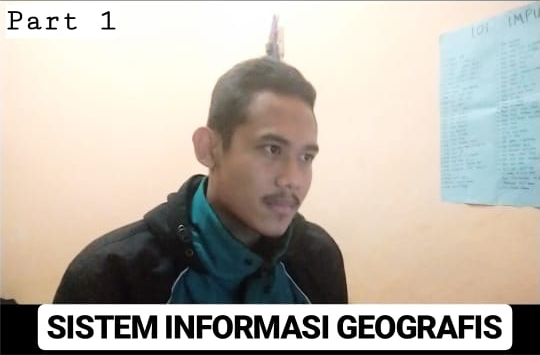
\includegraphics[width=4cm]{figures/1174021/2.png}
	\centering
	\caption{Video.}
\end{figure}

\begin{itemize}
	\item \href{https://www.youtube.com/watch?v=Dw8NGQUF-YQ} {Klik Disini saja !}
\end{itemize}

\subsection{Plagiarism}
\begin{figure}[H]
	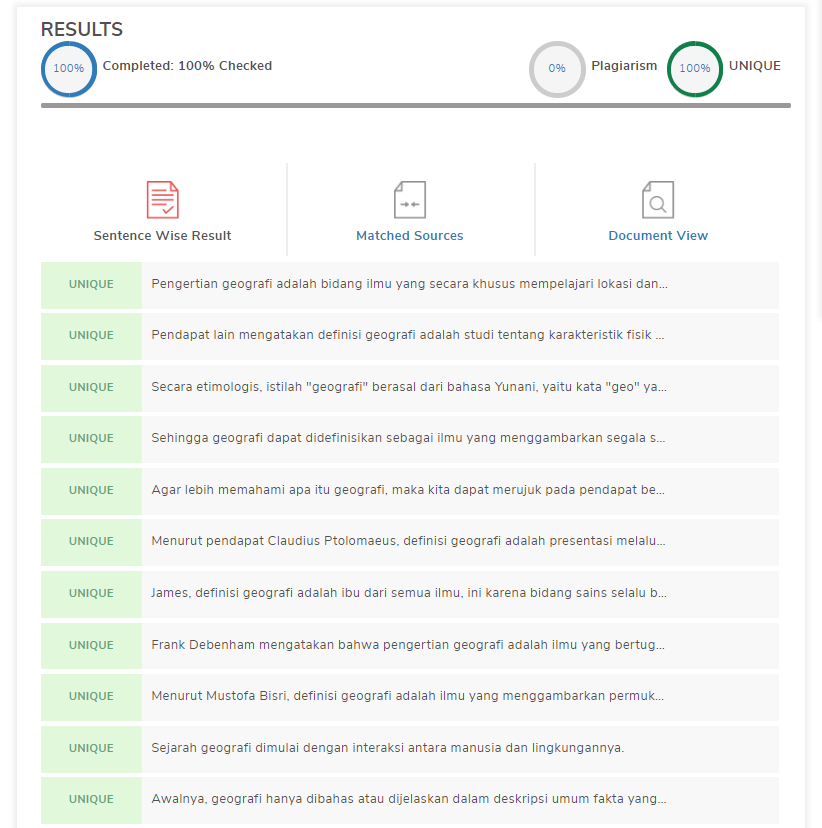
\includegraphics[width=4cm]{figures/1174021/buktiplagi1.png}
	\centering
	\caption{Bukti Tidak Melakukan Plagiat 1}
\end{figure}

\begin{figure}[H]
	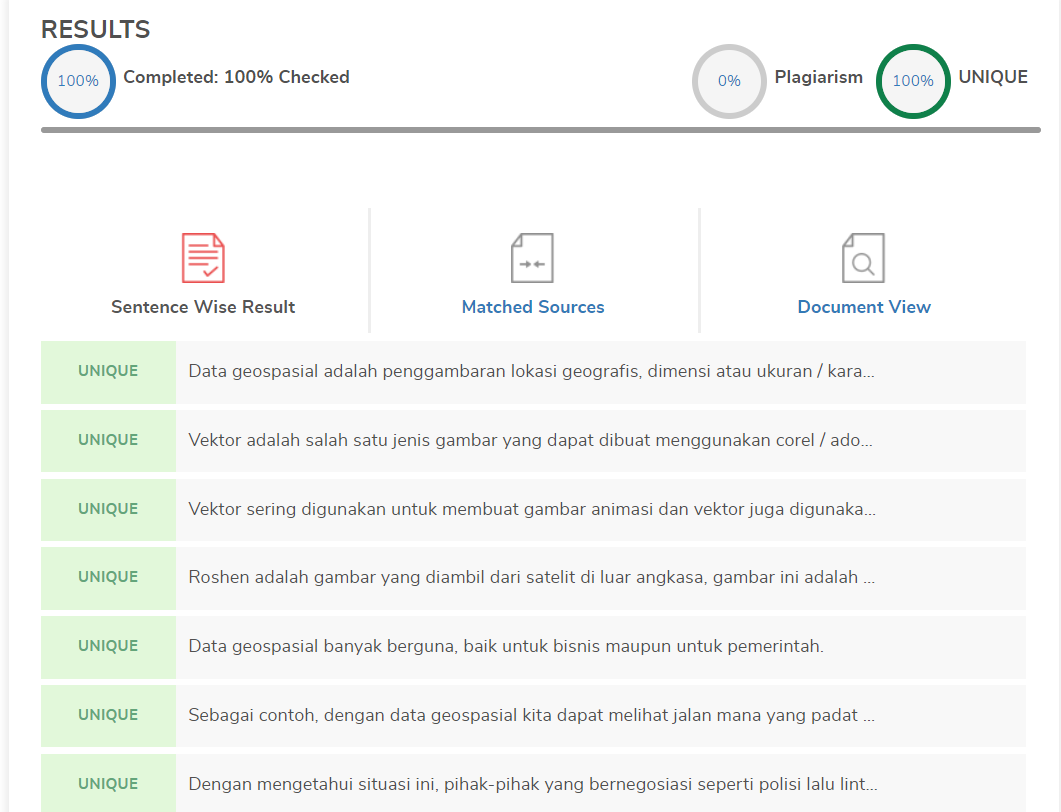
\includegraphics[width=4cm]{figures/1174021/buktiplagi2.png}
	\centering
	\caption{Bukti Tidak Melakukan Plagiat 2}
\end{figure}




%\section{Nico Ekklesia Sembiring (1174096)}
\subsection{Pengertian}
Sistem Informasi Geografis terdiri atas 3 kata. Yaitu Sistem, Informasi, dan Geografis. \hfill\break
SISTEM\hfill\break
Pada umumnya sistem diartikan sebagai suatu kesatuan yang terdiri atas komponen maupun elemen yang saling berinteraksi, saling berkaitan, atau saling bergantung sehingga membentuk keseluruhan yang kompleks.\hfill\break
INFORMASI\hfill\break
Informasi merupakan bentuk data yang telah diproses menjadi bentuk yang memiliki arti bagi penerima dan dapat berupa fakta, suatu nilai yang bermanfaat. Pada bagian ini ada suatu proses transformasi data menjadi suatu informasi yaitu input- proses -output.\hfill\break
GEOGRAFI\hfill\break
Geografi adalah ilmu yang mempelajari tentang lokasi serta persamaan dan perbedaan variasi keruangan atas fenomena fisik dan manusia di atas permukaan bumi. Geografi memiliki definisi lain yaitu ilmu yang mempelajari perbedaan dan persamaan terhadap fenomena yang terjadi pada geosfer melalui sudut pandang kewilayahan dan lingkungan dalam konteks keruangan.\hfill\break
SISTEM INFORMASI\hfill\break
Pada umumnya sistem informasi diartikan sebagai suatu sistem terintegrasi yang dapat menyediakan informasi yang bermanfaat untuk kepentingan pengguna, untuk menyediakan informasi untuk mendukung operasi, manajemen dalam suatu organisasi. Sistem ini memanfaatkan perangkat keras dan perangkat lunak komputer, prosedur manual, model manajemen dan basis data\hfill\break
SISTEM INFORMASI GEOGRAFIS\hfill\break
Pengertian dari Sistem Informasi Geografis (GIS) pada umumnya adalah sistem informasi khusus yang digunakan untuk melakukan pengelolaan data yang memiliki informasi geospasial. SIG juga merupakan sejenis perangkat lunak yang dapat digunakan untuk pemasukan, penyimpanan, manipulasi, menampilkan, dan keluaran informasi geografis berikut atribut – atributnya. SIG biasa digunakan untuk memberi nilai, dengan cara melakukan pengaturan dan memperlihatkan data secara tepat, menggabungkan dengan data lain, melakukan analisis terhadap data, dan menghasilkan data baru yang berguna, pada gilirannya SIG dapat membantu untuk pengambilan keputusan. Sistem Informasi Geografi dibagi menjadi dua kelompok yaitu sistem manual (analog), dan sistem otomatis (yang berbasis digital komputer). Perbedaan yang paling mendasar terletak pada cara pengelolaannya.\hfill\break

\subsection{Sejarah}
Sejarah GIS dimulai dari awal tahun 1960-an dimana terjadi perkembangan yang semakin pesat dalam ilmu komputer sehingga siap untuk digunakan pada bidang lain di luar militer. Ahli meteorologi, geologi, dan geofisika mulai menggunakan teknologi komputer dalam , melakukan pembuatan peta.\hfill\break
Pada tahun 1963 di Kanada terbentuk CGIS (Canadian Geographic Information System), dan selanjutnya menjadi SIG pertama di dunia. Kemudian 2 tahun setelahnya di Amerika Serikat dioperasikan sistem serupa yang bernama MIDAS yang biasa digunakan untuk memproses data-data sumber daya alam.\hfill\break
Seiring dengan berkembangnya teknologi, GIS juga mengalami perubahan ke arah yang lebih baik. \hfill\break
Berikut ini merupakan sejarah perkembangan GIS dari waktu ke waktu :\hfill\break
\begin{itemize}
	\item Pada 35000 tahun yang lalu, para pemburu Cro-Magnon menggambar hewan mangsa mereka di dinding gua Lascaux, Perancis, tidak hanya hewan mangsa, tetapi juga garis yang dipercaya sebagai rute migrasi hewan-hewan tersebut. Catatan penemuan awal ini sejalan dengan dua elemen struktur pada sistem informasi gegrafis modern sekarang ini, arsip grafis yang terhubung ke database atribut.\hfill\break
	\item Pada tahun 1700-an mulai diterapkan teknik survey modern untuk pemetaan topografis, penerapan ini termasuk juga versi awal pemetaan tematis, misalnya untuk keilmuan atau data sensus.\hfill\break
	\item Pada awal abad ke-20 diperlihatkan pengembangan “litografi foto” dimana peta tersebut dipisahkan menjadi beberapa lapisan (layer). Perkembangan perangkat keras komputer yang dipacu oleh penelitian senjata nuklir membawa aplikasi pemetaan menjadi multifungsi pada awal tahun 1960-an.\hfill\break
	\item Awal pengembangan SIG dimana mulai diterapkan di Ottawa, Ontario oleh Departemen Energi, Pertambangan dan Sumber Daya terjadi pada Tahun 1967.  Sistem ini dikembangkan oleh Roger Tomlinson, yang kemudian disebut sebagai CGIS (Canadian GIS – SIG Kanada),  sistem ini biasa digunakan untuk menyimpan, menganalisis dan mengolah data yang dikumpulkan dalam rangka kegiatan Inventarisasi Tanah Kanada (CLI – Canadian land Inventory). Hal ini merupakan sebuah inisiatif yang dilakukan mengetahui kemampuan suatu lahan di wilayah pedesaan Kanada dengan melakukan pemetaan berbagai informasi pada tanah, pertanian, pariwisata, alam bebas, unggas dan penggunaan tanah pada skala 1:250000. Faktor pemeringkatan klasifikasi juga diterapkan untuk keperluan analisis.\hfill\break
	\item GIS dengan gvSIG.CGIS merupakan sistem pertama di dunia dimana sistem ini merupakan hasil dari perbaikan yang sebelumnya telah memiliki, penghitungan, kemampuan timpang susun (overlay), pendigitalan/pemindaian (digitizing/scanning), mendukung sistem koordinat national yang terbentang di atas wilayah benua Amerika ,  hingga memasukkan garis dalam sebagai arc yang memiliki topologi dan menyimpan atribut dan informasi lokasional pada berkas terpisah. p, seorang geografer bernama Roger Tomlinson kemudian disebut “Bapak SIG”.\hfill\break
	\item CGIS bertahan sampai tahun 1970-an dan memakan waktu lama untuk penyempurnaan setelah pengembangan awal, dan tidak bisa bersaing denga aplikasi pemetaan komersil yang dikeluarkan beberapa vendor seperti Intergraph. Perkembangan perangkat keras mikro komputer memacu vendor lain seperti ESRI dan CARIS berhasil membuat banyak fitur SIG, menggabung pendekatan generasi pertama pada pemisahan informasi spasial dan atributnya, dengan pendekatan generasi kedua pada organisasi data atribut menjadi struktur database. Terjadinya perkembangan teknologi industri pada tahun 1980-an dan 1990-an memacu lagi pertumbuhan SIG pada workstation UNIX dan komputer pribadi. Pada akhir abad ke-20,  terjadi pertumbuhan yang cepat pada berbagai sistem yang dikonsolidasikan dan distandarisasikan menjadi platform lebih sedikit, serta para pengguna mulai mengekspor menampilkan data SIG lewat internet, yang membutuhkan standar pada format data dan transfer.
\end{itemize}
\subsection{Koordinat}
Untuk menggambarkan permukaan bumi yang berbentuk seperti bola ke dalam bentuk peta, diperlukan sebuah persamaan matematis yang dapat membantu mentransformasikan gambaran permukaan bumi. Persamaan ini disebut dengan sistem koordinat. Koordinat merupakan ciri khas utama dari GIS karena sistem koordinat ini yang dapat menunjukkan referensi geografis pada data data GIS. Dapat dikatakan bahwa sistem koordinat merupakan suatu pendekatan dalam mendefenisikan posisi data data GIS diatas permukaan bumi.\hfill\break
Dalam sistem koordinat, posisi objek pada permukaan bumi didefinisikan berdasarkan garis lintang(latitude) dan garis bujur(longitude). Garis lintang merupakan garis horizontal yang mengukur sudut antara satu titik dengan garis equator(garis khatulistiwa). Sedangkan garis bujur merupakan garis vertical yang mengukur sudut suatu titik dengan titik nol bumi, yaitu Greenwich Meridian, London\hfill\break
\begin{figure}[H]
	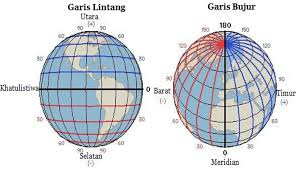
\includegraphics[width=4cm]{figures/1174096/1/koordinat2.jpg}
	\centering
	\caption{koordinat}
\end{figure}
Garis lintang terbagi menjadi 2, yaitu lintang utara dan lintang selatan dan garis bujur terbagi menjadi bujur timur dan bujur barat. Adanya kombinasi antara garis lintang dan garis bujur membentuk suatu koordinat lokasi di permukaan bumi dengan garis lintang sebagai sumbu x dan garis bujur sebagai sumbu y jika digambarkan dalam koordinat kartesius.
\begin{figure}[H]
	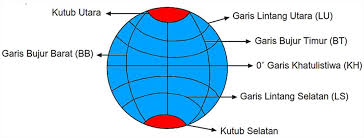
\includegraphics[width=4cm]{figures/1174096/1/lintangbujur.jpg}
	\centering
	\caption{garis lintang dan garis bujur}
\end{figure}
\begin{figure}[H]
	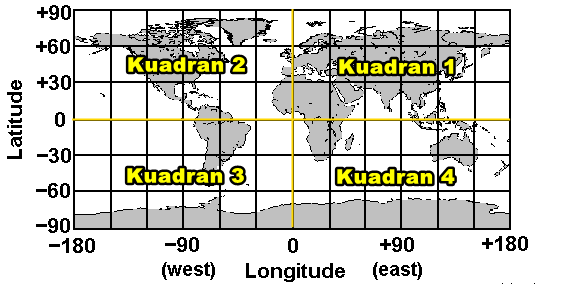
\includegraphics[width=4cm]{figures/1174096/1/Lintangbujurkuadran.png}
	\centering
	\caption{koordinat kartesius}
\end{figure}
\subsection{Data Geospasial}
Data Geospasial adalah data tentang aspek fisik dan administratif dari sebuah objek geografis.\hfill\break
Aspek fisik yang dimaksud mencakup bentuk anthropogenic dan bentuk alam baik yang terdapat di permukaan maupun di bawah permukaan bumi. Bentuk anthropogenic mengandung di dalamnya fenomena budaya seperti jalan, rel kereta api, bangunan, jembatan, dan sebagainya. Bentuk alam tentu saja adalah sungai, danau, pantai, daratan tinggi, dan sebagainya. \hfill\break
\begin{figure}[H]
	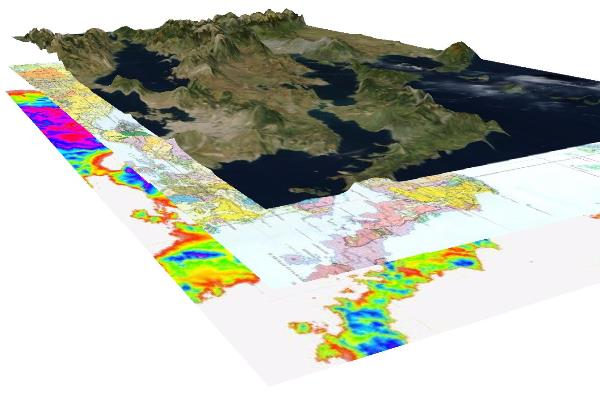
\includegraphics[width=4cm]{figures/1174096/1/consult_3.jpg}
	\centering
	\caption{aspek fisik}
\end{figure}
Sedangkan aspek administratif adalah pembagian atau pembatasan sosio-kultural yang dibuat oleh suatu organisasi atau badan untuk keperluan pengaturan dan pemakaian sumberdaya alam. Hal lain yang digolongkan kedalam aspek administratif ini adalah batas negara, zona, pembagian wilayah administrasi, kode pos, batas kepemilikan tanah, dan sebagainya.\hfill\break
\begin{figure}[H]
	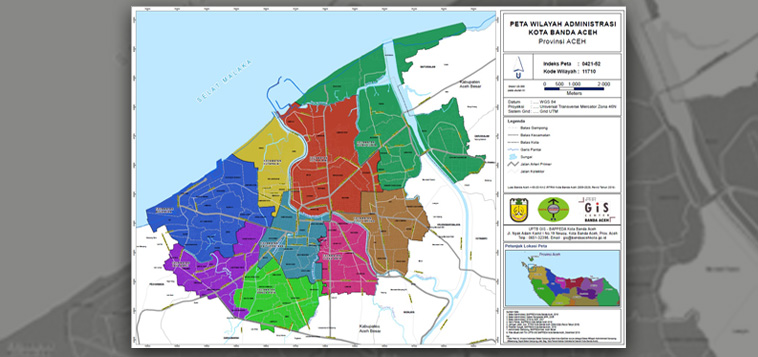
\includegraphics[width=4cm]{figures/1174096/1/PETA.jpg}
	\centering
	\caption{aspek administratif}
\end{figure}
Terdapat dua metode yang pada umumnya digunakan untuk menampilkan fitur geografis ke dalam GIS atau Sistem Informasi Geografis.\hfill\break 
\begin{itemize}
	\item Pertama, dengan struktur data vektor (vector data structure) yang terdiri dari sebuah gambaran titik geografis, baik yang berupa tanda titik, garis, maupun poligon. Struktur data vector biasa digunakan untuk menampilkan secara terpisah fitur geografis seperti batas administratif, jalan, bangunan, dan sungai. Sebuah objek grafis biasanya dikaitkan dengan informasi yang mengandung penjelasan tentang atribut objek itu, dan informasi ini bisa saja disimpan di dalam berkas spreadsheets atau pangkalan data terpisah.\hfill\break
	\item Kedua, dengan struktur data raster (raster data structure), terdiri dari serangkaian sel atau pixels yang biasa dipakai untuk menggambarkan data gambar sebagai data yang berkesinambungan. Dalam struktur data yang demikian, ada unsur resolusi sebagai ukuran dari dimensi fitur geografis yang terwakili dalam bentuk pixel. Biasanya data raster ini dipakai untuk citra satelit, ortografi digital, model elevasi digital (digital elevation models, DEM), peta digital, dan sebagainya.
\end{itemize}
\begin{figure}[H]
	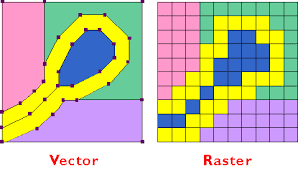
\includegraphics[width=4cm]{figures/1174096/1/vektordanraster.png}
	\centering
	\caption{data vektor dan raster}
\end{figure}
\subsection{Link}
\href{https://youtu.be/94y4uCmKc1Q}{Untuk selengkapnya lihat disini}

\subsection{Plagiarism}
\begin{figure}[H]
	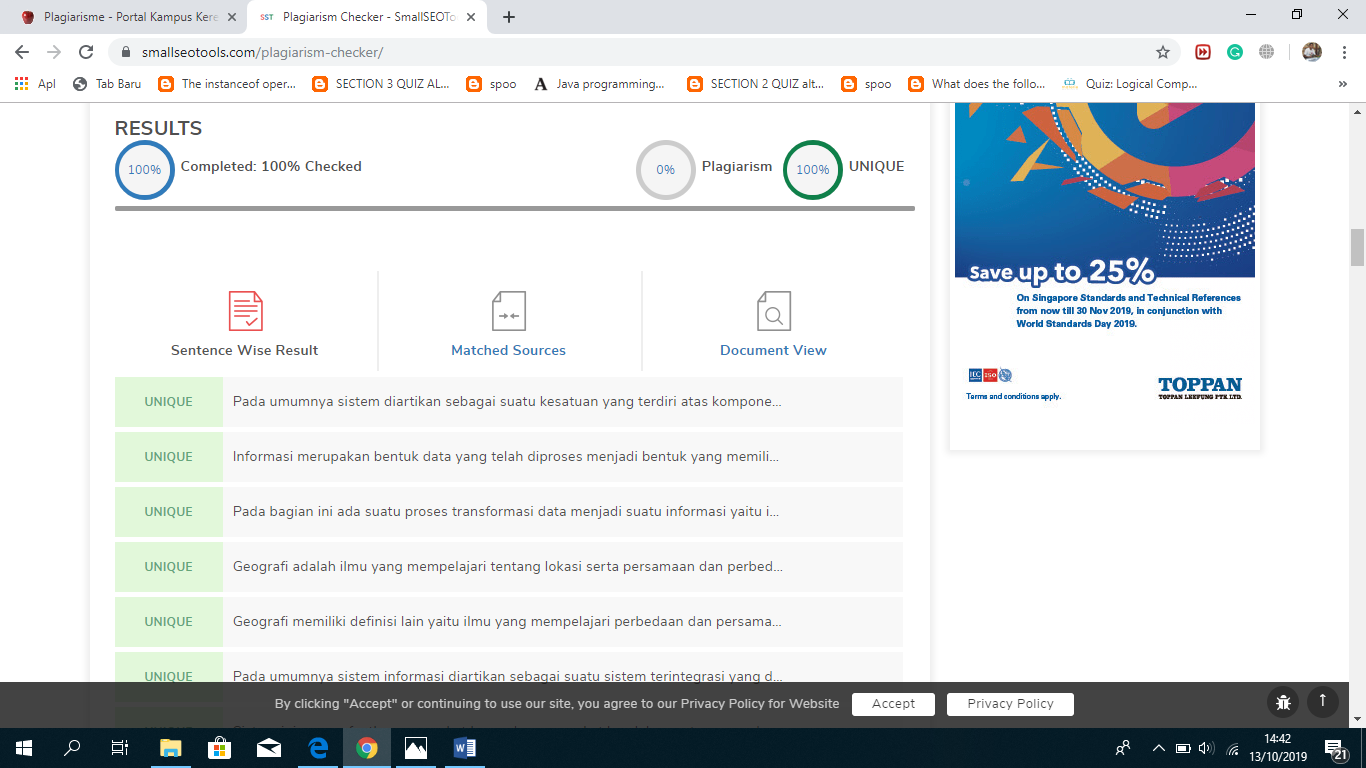
\includegraphics[width=4cm]{figures/1174096/1/plagiarisme.png}
	\centering
	\caption{cek plagiarisme}
\end{figure}

\href{https://www.google.com/}{klik me}
%\section{ONIWALDUS BERE MALI (1174005)}
\subsection{Pengertian}
Sistem Informasi Geografis (SIG) atau Geographic Information System (GIS) adalah sustem informai khusu yang mengelola data yang memiliki informasi spasial yaitu bereferensi keruangan. Atau lebih singkatnya, sistem informasi geografis adalah h sistem komputer yang mempunyai kemampuan untuk membangun, menyimpan, mengelola dan menampilkan informasi berefrensi geografis, misalnya data diidentifikasi menurut lokasinya dalam sebuah database.
Teknologi Sistem Informasi Geografis digunakan untuk investigasi ilmiah, pengelolaan sumber daya, perencanaan pembangunan, kartografi dan perencanaan rute. Contohnya SIG dapat digunakan perencana untuk membantu menghitung waktu tanggap darurat saat terjadi bencana alam secara cepat dan lain sebagainya.

\subsection{Sejarah}
35000 tahun yang lalu, di dinding gua Lascaux, Perancis, para pemburu Cro-Magnon menggambar hewan mangsa mereka, dan juga garis yang dipercaya sebagai rute migrasi hewan-hewan tersebut. Catatan awal ini sejalan dengan dua elemen struktur pada sistem informasi gegrafis modern sekarang ini, arsip grafis yang terhubung ke database atribut.
Pada tahun 1700-an teknik survey modern untuk pemetaan topografis diterapkan, termasuk juga versi awal pemetaan tematis, misalnya untuk keilmuan atau data sensus.
Awal abad ke-20 memperlihatkan pengembangan “litografi foto” dimana peta dipisahkan menjadi beberapa lapisan (layer). Perkembangan perangkat keras komputer yang dipacu oleh penelitian senjata nuklir membawa aplikasi pemetaan menjadi multifungsi pada awal tahun 1960-an.
Tahun 1967 merupakan awal pengembangan SIG yang bisa diterapkan di Ottawa, Ontario oleh Departemen Energi, Pertambangan dan Sumber Daya. Dikembangkan oleh Roger Tomlinson, yang kemudian disebut CGIS (Canadian GIS – SIG Kanada), digunakan untuk menyimpan, menganalisis dan mengolah data yang dikumpulkan untuk Inventarisasi Tanah Kanada (CLI – Canadian land Inventory) – sebuah inisiatif untuk mengetahui kemampuan lahan di wilayah pedesaan Kanada dengan memetakaan berbagai informasi pada tanah, pertanian, pariwisata, alam bebas, unggas dan penggunaan tanah pada skala 1:250000. Faktor pemeringkatan klasifikasi juga diterapkan untuk keperluan analisis.
GIS dengan gvSIG.
CGIS merupakan sistem pertama di dunia dan hasil dari perbaikan aplikasi pemetaan yang memiliki kemampuan timpang susun (overlay), penghitungan, pendijitalan/pemindaian (digitizing/scanning), mendukung sistem koordinat national yang membentang di atas benua Amerika , memasukkan garis sebagai arc yang memiliki topologi dan menyimpan atribut dan informasi lokasional pada berkas terpisah. Pengembangya, seorang geografer bernama Roger Tomlinson kemudian disebut “Bapak SIG”.

\subsection{Koordinat}
Penginderaan Jauh
Penginderaan jauh adalah metode pengambilan informasi dan pencatatan rupabumi suatu wilayah dengan menggunakan wahana tertentu.Sesuai dengan namanya, surveyor yang menggunakan penginderaan jauh umumnya berlokasi jauh atau tidak langsung berada di wilayah survey. Hal ini dapat terjadi karena kemajuan teknologi pada bidang foto udara, sensor, pesawat, serta satelit.Penginderaan jauh umumnya dilakukan dengan menggunakan foto udara dari pesawat, foto satelit, atau teknologi drone.
GPS atau Global Positioning System adalah sistem penentuan lokasi global yang memanfaatkan satelit untuk melakukan triangulasi lokasi perangkat.
Global positioning system berkerja dengan cara menerima sinyal dari satelit yang nantinya akan digunakan untuk melakukan triangulasi lokasi. Oleh karena itu, GPS hanya dapat berfungsi secara akurat jika terdapat 3 atau lebih satelit yang mengirimkan sinyal.
Selain itu, GPS juga harus memiliki koneksi sinyal yang bagus dengan satelit tersebut agar dapat memprediksi lokasi secara akurat.Sekarang, GPS sudah memiliki akurasi dibawah 10m sehingga mengurangi galat saat melakukan perhitungan atau navigasi. GPS navigais tertentu bahkan sudah mencapai akurasi dibawah 3-5m, sedangkan GPS untuk survei dan pemetaan sudah memiliki akurasi dalam rentang milimeter.Meskipun begitu, perangkat GPS yang memiliki kualitas dan akurasi tinggi sangat sulit didapatkan dan memiliki harga yang mahal. Oleh karena itu, tidak semua orang dapat mengakses sebuah GPS.Sistem informasi geografis memiliki banyak manfaat, 
Koordinat adalah suatu titik yang didapatkan dari hasil perpotongan dari garis latitude (lintang) dengan garis bujur (longitude) sehingga akan menunjukan lokasi pada suatu daerah. Umumnya koordinat dibedakan menjadi koordinat Geographic dan Universal Transver Mercator (UTM). Pada Koordinat Geogprahic dibedakan menjadi tiga berdasarkan satuannya yaitu :
1.	Degree, Decimal (DD,DDDD) Contoh : S 3.56734 E 104.67235
2.	Degree, Minute (DD MM,MMMM) Contoh : S 3⁰ 43,5423’ E 104 33,6445’
3.	Degree, Minute, Second (DD MM SS,SS) Contoh : S 3⁰ 43’ 45,22” E104 33’ 33,25”
Pada Bujur/Longitude (X) merupakan garis yang perpindahannya secara vertical dan pada Lintang/Lattitude (Y) merupakan garis yang mempunyai perpindahan secara horizontal, pada (Gambar 1) menjelaskan perpotongan antara garis bujur dan garis lintang akan membentuk suatu titik pertemuan yang biasa disebut dengan titik koordinat. Pada Sistem Koordinat UTM biasanya terdapat pembagian waktu berdasarkan zonasinya, di Indonesia sendiri terdapat 16 pembagian zonasi waktu, pada Gambar 2 menjelaskan pembagian zonasi waktu dimana terdapat garis yang memisahkan dari garis khatulistiwa. Untuk Daerah yang berada di atas garis khatulistiwa akan mempunyai Kode N sedangkan yang berada dibawah khatulistiwa akan mempunyai kode S.Saat penggunaan GPS biasanya terdapat pengaturan untuk melakukan konversi pada satuan koordinat sehingga memudahkan pengguna berdasarkan kebutuhan yang diinginkan. Konversi pun dapat dilakukan dengan merubah satuan Koordinat Geografis DD MM SS,SS menjadi DD,DDDD ataupun sebaliknya.

\subsection{Data Geospasial}
Data geospasial adalah kumpulan fakta yang berupa informasi tentang ruang kebumian (geospasial) yang menunjukan lokasi atau posisi dari suatu tempat atau objek yang direpresentasikan pada sebuah garis titik koordinat. Data geospasial dibagi menjadi 2 yaitu:
Data Vector
Dalam bentuk data vector bagian objek dibumi ditampilkan sebagai kumpulan titik , garis dan polygon dimana sekumpulan tiitik yang saling terhubung akan membentuk garis dan garis yang saling terhubung antara titik awal dan titik akhir dengan nilai koordinat ynag sama akan membentuk polygon . Data vector dibagi menjadi 2 yaitu :
Culture
Culture memaparkan atau menampilkan data geospasial yang disertai dengan nama atribut atau memberikan keterangan atas nama dari objek di bumi. Contohnya nama dari suatu Negara, indicator batas air (keterangan kedalaman air laut), nama provinsi, daerah, wilayah dsb.
populated-culture
Physical
Physical memaparkan atau menampilkan data geospasial mengenai bentuk fisiknya atau gambaran tentang objek-objek alam yang ada dibumi.
2. Data Raster
Data raster menampilkan permukaan bumi seperti bentuk aslinya atau seperti dalam peta asli yang terlihat jelas dari setiap objek dengan keadaan alamnya. Data raster dibentuk atau menampilkan objek berupa elemen matriks atau grid , data raster digunakan untuk merepresentasikan objek dari data geospasial mengenai batas-batas yang berubah, ketinggian tanah

\subsection{Link}
\href{https://youtu.be/GYiF4K6OzEg}{klik disini}

\subsection{Plagiarism}
\begin{figure}[H]
	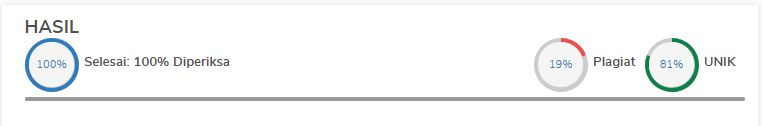
\includegraphics[width=4cm]{figures/1174005/ONI.JPG}
	\centering
	\caption{Gambar plagiat tugas 1}
\end{figure}

%\section{Muhammad Tomy (1174031)}
\subsection{Pengertian}
SIG atau Sistem Informasi Geografis dalam bahasa Inggris disebut Geographic Information System disingkat GIS adalah sistem informasi khusus yang mengelola data yang memiliki informasi spasial. SIG juga bias diartikan  dalam arti yang lebih sempit, adalah sistem komputer yang memiliki kemampuan untuk membangun, menyimpan, mengelola dan menampilkan informasi berefrensi geografis, misalnya data yang diidentifikasi menurut lokasinya, dalam sebuah database. Para praktisi juga memasukkan orang yang membangun dan mengoperasikannya dan data sebagai bagian dari sistem ini. Teknologi Sistem Informasi Geografis dapat digunakan untuk investigasi ilmiah, pengelolaan sumber daya, perencanaan pembangunan, kartografi dan perencanaan rute. Misalnya, SIG bisa membantu perencana untuk secara cepat menghitung waktu tanggap darurat saat terjadi bencana alam, atau SIG dapat digunaan untuk mencari lahan basah (wetlands) yang membutuhkan perlindungan dari polusi.


\subsection{Sejarah}
35000 tahun yang lalu, di dinding gua Lascaux, Perancis, para pemburu Cro-Magnon menggambar hewan mangsa mereka, dan juga garis yang dipercaya sebagai rute migrasi hewan-hewan tersebut. Catatan awal ini sejalan dengan dua elemen struktur pada sistem informasi gegrafis modern sekarang ini, arsip grafis yang terhubung ke database atribut.
Pada tahun 1700-an teknik survey modern untuk pemetaan topografis diterapkan, termasuk juga versi awal pemetaan tematis, misalnya untuk keilmuan atau data sensus. Awal abad ke-20 memperlihatkan pengembangan “litografi foto” dimana peta dipisahkan menjadi beberapa lapisan (layer). Perkembangan perangkat keras komputer yang dipacu oleh penelitian senjata nuklir membawa aplikasi pemetaan menjadi multifungsi pada awal tahun 1960-an.
Tahun 1967 merupakan awal pengembangan SIG yang bisa diterapkan di Ottawa, Ontario oleh Departemen Energi, Pertambangan dan Sumber Daya. Dikembangkan oleh Roger Tomlinson, yang kemudian disebut CGIS (Canadian GIS – SIG Kanada), digunakan untuk menyimpan, menganalisis dan mengolah data yang dikumpulkan untuk Inventarisasi Tanah Kanada (CLI – Canadian land Inventory) – sebuah inisiatif untuk mengetahui kemampuan lahan di wilayah pedesaan Kanada dengan memetakaan berbagai informasi pada tanah, pertanian, pariwisata, alam bebas, unggas dan penggunaan tanah pada skala 1:250000. Faktor pemeringkatan klasifikasi juga diterapkan untuk keperluan analisis. CGIS merupakan sistem pertama di dunia dan hasil dari perbaikan aplikasi pemetaan yang memiliki kemampuan timpang susun (overlay), penghitungan, pendijitalan/pemindaian (digitizing/scanning), mendukung sistem koordinat national yang membentang di atas benua Amerika , memasukkan garis sebagai arc yang memiliki topologi dan menyimpan atribut dan informasi lokasional pada berkas terpisah. Pengembangya, seorang geografer bernama Roger Tomlinson kemudian disebut “Bapak SIG”. CGIS bertahan sampai tahun 1970-an dan memakan waktu lama untuk penyempurnaan setelah pengembangan awal, dan tidak bisa bersaing denga aplikasi pemetaan komersil yang dikeluarkan beberapa vendor seperti Intergraph. Perkembangan perangkat keras mikro komputer memacu vendor lain seperti ESRI, CARIS, MapInfo dan berhasil membuat banyak fitur SIG, menggabung pendekatan generasi pertama pada pemisahan informasi spasial dan atributnya, dengan pendekatan generasi kedua pada organisasi data atribut menjadi struktur database. Perkembangan industri pada tahun 1980-an dan 1990-an memacu lagi pertumbuhan SIG pada workstation UNIX dan komputer pribadi. Pada akhir abad ke-20, pertumbuhan yang cepat di berbagai sistem dikonsolidasikan dan distandarisasikan menjadi platform lebih sedikit, dan para pengguna mulai mengekspor menampilkan data SIG lewat internet, yang membutuhkan standar pada format data dan transfer.Indonesia sudah mengadopsi sistem ini sejak Pelita ke-2 ketika LIPI mengundang UNESCO dalam menyusun “Kebijakan dan Program Pembangunan Lima Tahun Tahap Kedua (1974-1979)” dalam pembangunan ilmu pengetahuan, teknologi dan riset.



\subsection{Koordinasi}
Koordinat adalah suatu titik yang didapatkan dari hasil perpotongan dari garis latitude (lintang) dengan garis bujur (longitude) sehingga akan menunjukan lokasi pada suatu daerah. Umumnya koordinat dibedakan menjadi koordinat Geographic dan Universal Transver Mercator (UTM). Pada Koordinat Geogprahic dibedakan menjadi tiga berdasarkan satuannya yaitu :
\begin{itemize}
	\item Degree, Decimal(DD, DDDD) contoh S 4.56734 E 102.67235
	\item Degree,Minute(DD MM,MMMM) contoh S 4 42,5423’ E 105 34,6445’
	\item Degree, Minute, Second(DD MM SS,SS) contoh : S 4 43’ 45,22 E 103 33’ 33,25
\end{itemize}
Pada Bujur/Longitude (X) merupakan garis yang perpindahannya secara vertical dan pada Lintang/Lattitude (Y) merupakan garis yang mempunyai perpindahan secara horizontal.

\subsection{Geospasial}
Data geospasial adalah kumpulan fakta yang berupa informasi tentang ruang kebumian (geospasial) yang menunjukan lokasi atau posisi dari suatu tempat atau objek yang direpresentasikan pada sebuah garis titik koordinat. Data geospasial dibagi menjadi 2 yaitu:
\begin{itemize}
	\item Vektor
	Dalam bentuk data vector bagian objek dibumi ditampilkan sebagai kumpulan titik , garis dan polygon dimana sekumpulan tiitik yang saling terhubung akan membentuk garis dan garis yang saling terhubung antara titik awal dan titik akhir dengan nilai koordinat ynag sama akan membentuk polygon . 

	\item Raster
	Data raster menampilkan permukaan bumi seperti bentuk aslinya atau seperti dalam peta asli yang terlihat jelas dari setiap objek dengan keadaan alamnya. Data raster dibentuk atau menampilkan objek berupa elemen matriks atau grid , data raster digunakan untuk merepresentasikan objek dari data geospasial mengenai batas-batas yang berubah, ketinggian tanah dsb.
\end{itemize}


\subsection{Link}
\href{https://youtu.be/oJ2smVdIph4}{Sistem Informasi Geografis}

\subsection{Plagiarism}
\begin{figure}[H]
	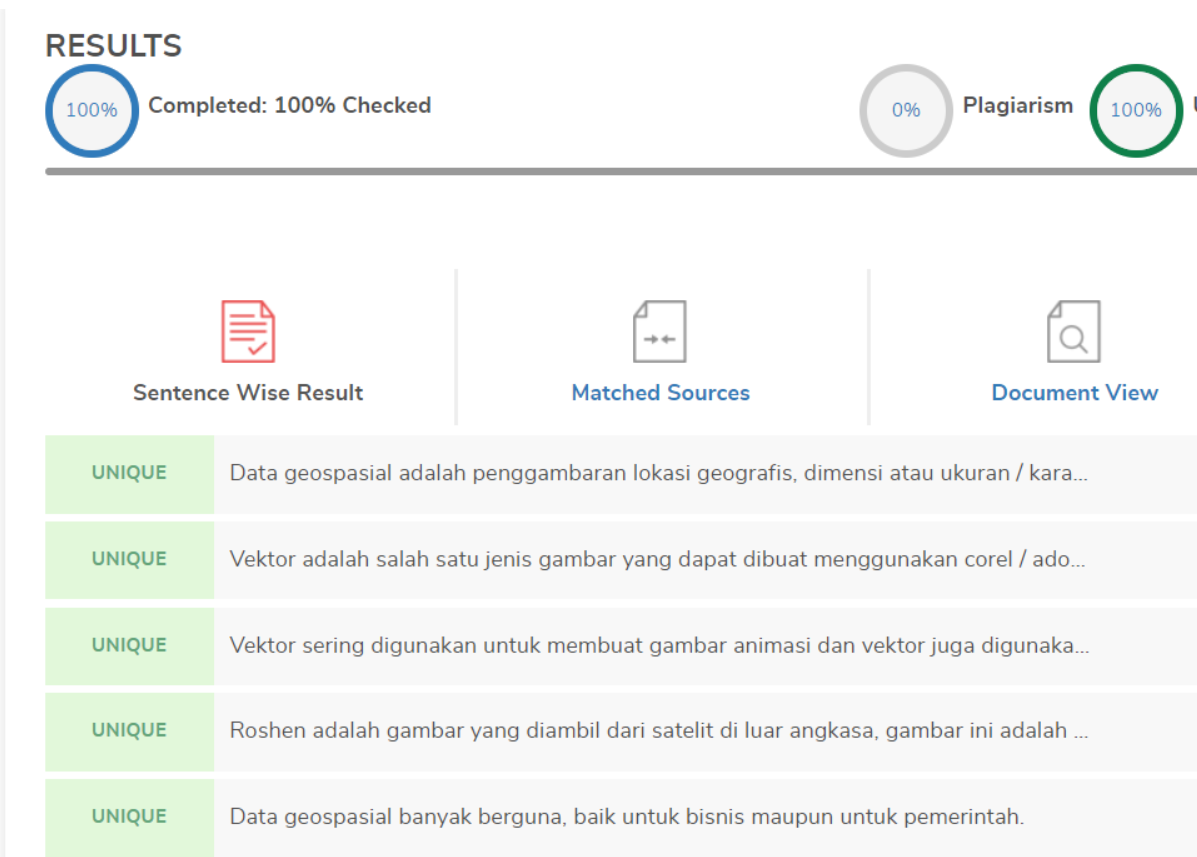
\includegraphics[width=4cm]{figures/1174031/plagiat.png}
	\centering
	\caption{Plagiarism 1174031}
\end{figure}

%\section{MUH. RIFKY PRANANDA (1174017)}
\begin{figure}[H]
	
\includegraphics[width=4cm]{figures/1174017/gis1.JPG}
	\centering
	\caption{Contoh gambar.}
\end{figure}
\subsection{Pengertian}
Geografi adalah ilmu yang mempelajari tentang lokasi serta persamaan dan perbedaan variasi keruangan atas fenomena fisik, dan manusia di atas permukaan bumi. Kata geografi berasal dari Bahasa Yunani yaitu gêo "Bumi", dan graphein "tulisan" atau "menjelaskan". Para sarjana, praktisi, atau penulis di bidang geografi disebut geograf atau geografer.Geografi juga merupakan nama judul buku bersejarah pada subjek ini, yang terkenal adalah Geographia tulisan Klaudios Ptolemaios pada abad kedua.Geografi lebih dari sekadar kartografi, studi tentang peta. Geografi tidak hanya menjawab apa, dan di mana di atas muka bumi, tapi juga mengapa di situ, dan tidak di tempat lainnya, kadang diartikan dengan "lokasi pada ruang." Geografi mempelajari hal ini, baik yang disebabkan oleh alam atau manusia. Juga mempelajari akibat yang disebabkan dari perbedaan yang terjadi itu.
Sistem informasi geografis (SIG) adalah sistem yang didesain untuk menangkap, menyimpan, mengolah, menganalisa, serta mempresentasikan data spasial.Dengan menghubungkan berbagai jenis data yang awalnya dianggap tidak berhubungan, SIG dapat membantu manusia dalam berbagai aspek pekerjaan. Proses menghubungkan ini umumnya dilakukan dalam konteks lokasi (spasial) dan waktu (temporal) yang sama.
\begin{figure}[H]
	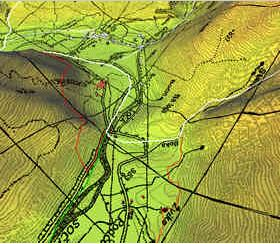
\includegraphics[width=4cm]{figures/1174017/gis.JPG}
	\centering
	\caption{Contoh gambar.}
\end{figure}
\subsection{Sejarah}
Pada awalnya, peta hanya memiliki satu atau dua informasi saja didalamnya, sehingga jika seorang analis ingin mendapatkan informasi tambahan, dia harus melakukan overlay.Salah satu proses overlay pertama yang juga dianggap sebagai penggunaan analisa spasial pertama secara sukses adalah oleh John Snow di London pada tahun 1854. Dia melakukan pemetaan terhadap lokasi orang-orang yang mengidap penyakit cholera dan menghubungkannya dengan peta penyediaan air minum London.Pada awal abad ke-20, penggunaan teknik photozincography mulai meluas. Teknik ini memungkinkan peta terdiri dari beberapa layer yang nantinnya dapat diubah secara mandiri dari layer lainnya. Hal ini berguna untuk melakukan overlay dan analisa peta sesuai dengan layer yang dibutuhkan.Pada teknik ini, layer-layer yang ada dibuat dari film plastik atau lapisan kertas kalkir sehingga dapat digabungkan menjadi satu peta besar. Namun, teknik ini belum dapat dianggap sebagai SIG karena tidak terdapat database yang menghubungkan peta-peta tersebut.Pada tahun 1960, Canada mengembangkan sistem SIG pertamanya yang disebut CGIS atau Canada Geographic Information System. Sistem ini digunakan untuk menyimpan, mengolah, dan menganalisa informasi yang dimiliki oleh badan pertanahan Canada.
\begin{figure}[H]
	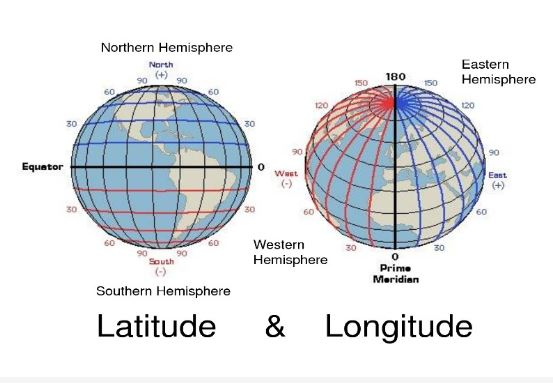
\includegraphics[width=4cm]{figures/1174017/gis2.JPG}
	\centering
	\caption{Contoh gambar.}
\end{figure}
\subsection{Koordinat}
Peta, Proyeksi Peta, Sistem Koordinat, Survei dan GPS 
   Data spasial yang dibutuhkan pada SIG dapat diperoleh dengan berbagai cara. Salah satunya melalui survei dan pemetaan, yaitu penentuan posisi/koordinat di lapangan. Berikut ini akan dijelaskan secara ringkas beberapa hal yang berkaitan dengan posisi/koordinat serta metode-metode untuk mendapatkan informasi posisi tersebut di lapangan
\subsubsection{peta}
Peta adalah gambaran sebagian atau seluruh muka bumi baik yang terletak di atas maupun di bawah permukaan dan disajikan pada bidang datar pada skala dan proyeksi tertentu (secara matematis). Karena dibatasi oleh skala dan proyeksi maka peta tidak akan pernah selengkap dan sedetail aslinya (bumi). Untuk itu diperlukan penyederhanaan dan pemilihan unsur yang akan ditampilkan pada peta.
\subsubsection{proyeksipeta}
Pada dasarnya bentuk bumi tidak datar, tapi mendekati bulat. Maka untuk menggambarkan sebagian muka bumi untuk kepentingan pembuatan peta, perlu dilakukan langkah-langkah agar bentuk yang mendekati bulat tersebut dapat didatarkan dan distorsinya dapat terkontrol. Caranya dengan melakukan proyeksi ke bidang datar.
\subsubsection{Yang menggunakan bidang proyeksi}
Bidang datar, Bidang kerucut, Bidang silinder
\subsubsection{Proyeksi Universal Tranverse Mercator}
Proyeksi UTM dibuat oleh US Army sekitar tahun 1940-an. Sejak saat itu proyeksi ini menjadi standar untuk pemetaan topografi
\subsubsection{Sistem kordinat UTM}
Untuk menghindari koordinat negatif, dalam proyeksi UTM setiap meridian tengah dalam tiap zone diberi harga 500.000 mT (meter timur). Untuk harga-harga ke arah utara, ekuator dipakai sebagai garis datum dan diberi harga 0 mU (meter utara). Untuk perhitungan ke arah selatan ekuator diberi harga 10.000.000 mU.

   Wilayah Indonesia (90° – 144° BT dan 11° LS – 6° LU) terbagi dalam 9 zone UTM. Artinya, wilayah Indonesia dimulai dari zone 46 sampai zone 54 (meridian sentral 93° – 141° BT).
\subsubsection{Metode penentuan posisi}
Metode penentuan posisi adalah cara untuk mendapatkan informasi koordinat suatu objek di lapangan, contohnya koordinat titik batas, koordinat batas persil tanah dan lain-lain. Metode penentuan posisi dapat dibedakan dalam dua bagian, yaitu metode penentuan posisi terestris dan metode penentuan posisi extra-terestris (satelit).
Pada metode terestris, penentuan posisi titik dilakukan dengan melakukan pengamatan terhadap target atau objek yang terletak di permukaan bumi. Beberapa contoh metode yang umum digunakan adalah:
metode poligon, metode pemikatan ke muka, metode pengikatan ke belakang dan lain lain.
\subsection{Data Geospasial}
\subsubsection{Data spasial}
Data spasial adalah data yang memiliki informasi lokasi pada data tersebut. Informasi lokasi ini umumnya berbentuk sistem koordinat baik itu koordinat geografis ataupun koordinat proyeksi.
Data spasial umumnya digunakan untuk menunjukkan lokasi dari suatu obyek/kenampakan pada dunia nyata.
Terdapat dua jenis data spasial yaitu vektor dan raster. Kedua jenis data ini memiliki perbedaan sifat dan kegunaannya. Oleh karena itu, penggunaannya sangat tergantung dengan kondisi dan hasil yang ingin dicapai.
\subsubsection{Data vektor}
Data vektor adalah data yang direpresentasikan dengan garis, titik, atau polygon. Data vektor dihasilkan dari digitasi data raster ataupun penggambaran langsung obyek dunia nyata pada peta. Oleh karena itu, data vektor lebih sulit dibuat dibandingkan dengan data raster.
\subsubsection{Data Raster}
Data raster adalah data yang direpresentasikan dengan piksel dalam sebuah grafik. Data raster dihasilkan langsung oleh foto udara maupun foto satelit. Oleh karena itu, secara umum, data raster lebih mudah dibuat dibandingkan dengan data vektor.
\subsubsection{Data Aspasial}
Data aspasial adalah data yang tidak memiliki informasi mengenai lokasi data tersebut. Data ini umumnya digunakan untuk membantu menjelaskan informasi yang terkandung pada data spasial.
Contoh data aspasial adalah data atribut suatu obyek. Misal pada suatu peta terdapat titik berwarna hitam pada koordinat tertentu, kita tidak akan tahu titik tersebut bermakna apa tanpa adanya penjelas yaitu legenda. Legenda adalah salah satu contoh data aspasial.
Sistem informasi geografis modern menggunakan data digital untuk proses analisa dan Y666penafsirannya. Berikut ini adalah beberapa metode pengumpulan data untuk analisa SIG.
Digitasi adalah proses mendigitalkan data yang bersifat fisik. Hal ini perlu dilakukan karena mayoritas data perpetaan masih berada dalam bentuk fisik seperti pada lembaran film atau kertas peta.
Proses ini dapat dilakukan dengan cara memasukkan data fisik seperti foto dan peta kedalam mesin, atau men-scan data tersebut dan mendigitasinya secara manual dengan aplikasi.Proses digitasi akan mengubah data raster menjadi data vektor yang dapat diolah dan dianalisa oleh aplikasi SIG.
Survey juga merupakan bagian yang sangat penting dari SIG. Survey meliputi aktivitas pengambilan data langsung di tempatSurvey menghasilkan data yang nantinya dapat langsung dimasukkan kedalam basis data SIG dengan menggunakan coordinate geometry (COGO).Meskipun telah ada teknologi penginderaan jauh, survey masih sangat dibutuhkan dalam proses pemetaan. Hal ini disebabkan oleh keberadaan informasi-informasi detail lokasi yang mungkin tidak dapat ditangkap dan digambarkan oleh penginderaan jauh.
\subsection{https://youtu.be/QSoJBLX-hQ0}
\subsection{Plagiarism}
\begin{figure}[H]
	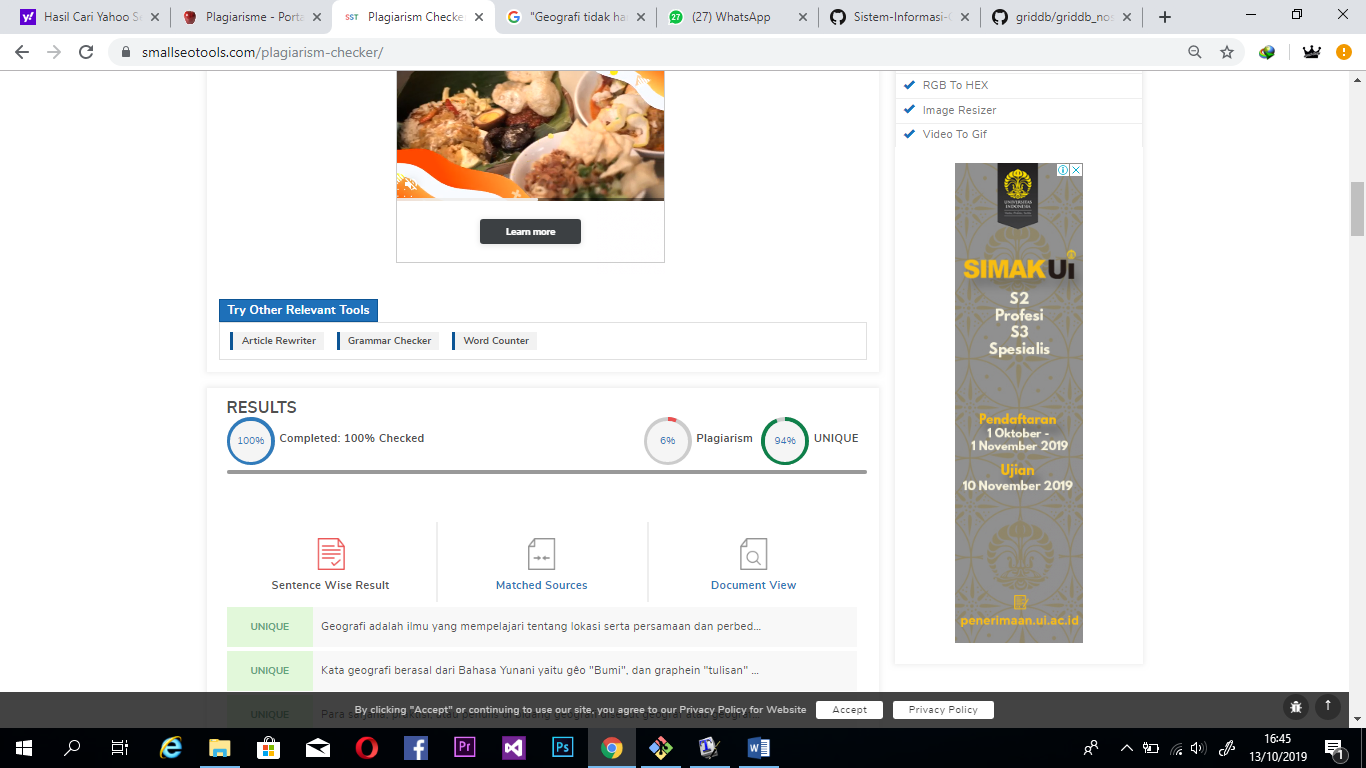
\includegraphics[width=4cm]{figures/1174017/plagiat.png}
	\centering
	\caption{plgt}
\end{figure}
%\section{SRI RAHAYU (1174015)}
\subsection{Pengertian SIG}
Geografi adalah ilmu yang mempelajari tentang lokasi serta persamaan dan perbedaan variasi keruangan atas fenomena fisik, dan manusia di atas permukaan bumi. Kata geografi berasal dari Bahasa Yunani yaitu gêo "Bumi", dan graphein "tulisan" atau "menjelaskan". Para sarjana, praktisi, atau penulis di bidang geografi disebut geograf atau geografer.Geografi juga merupakan nama judul buku bersejarah pada subjek ini, yang terkenal adalah Geographia tulisan Klaudios Ptolemaios pada abad kedua.Geografi lebih dari sekadar kartografi, studi tentang peta. Geografi tidak hanya menjawab apa, dan di mana di atas muka bumi, tapi juga mengapa di situ, dan tidak di tempat lainnya, kadang diartikan dengan "lokasi pada ruang." Geografi mempelajari hal ini, baik yang disebabkan oleh alam atau manusia. Juga mempelajari akibat yang disebabkan dari perbedaan yang terjadi itu.
Sistem informasi geografis (SIG) adalah sistem yang didesain untuk menangkap, menyimpan, mengolah, menganalisa, serta mempresentasikan data spasial.Dengan menghubungkan berbagai jenis data yang awalnya dianggap tidak berhubungan, SIG dapat membantu manusia dalam berbagai aspek pekerjaan. Proses menghubungkan ini umumnya dilakukan dalam konteks lokasi (spasial) dan waktu (temporal) yang sama.

\subsection{Sejarah SIG}
Pada awalnya, peta hanya memiliki satu atau dua informasi saja didalamnya, sehingga jika seorang analis ingin mendapatkan informasi tambahan, dia harus melakukan overlay.Salah satu proses overlay pertama yang juga dianggap sebagai penggunaan analisa spasial pertama secara sukses adalah oleh John Snow di London pada tahun 1854. Dia melakukan pemetaan terhadap lokasi orang-orang yang mengidap penyakit cholera dan menghubungkannya dengan peta penyediaan air minum London.Pada awal abad ke-20, penggunaan teknik photozincography mulai meluas. Teknik ini memungkinkan peta terdiri dari beberapa layer yang nantinnya dapat diubah secara mandiri dari layer lainnya. Hal ini berguna untuk melakukan overlay dan analisa peta sesuai dengan layer yang dibutuhkan.Pada teknik ini, layer-layer yang ada dibuat dari film plastik atau lapisan kertas kalkir sehingga dapat digabungkan menjadi satu peta besar. Namun, teknik ini belum dapat dianggap sebagai SIG karena tidak terdapat database yang menghubungkan peta-peta tersebut.Pada tahun 1960, Canada mengembangkan sistem SIG pertamanya yang disebut CGIS atau Canada Geographic Information System. Sistem ini digunakan untuk menyimpan, mengolah, dan menganalisa informasi yang dimiliki oleh badan pertanahan Canada.
Data Yang Digunakan dalam Sistem Informasi Geografis
Terdapat dua jenis data yang umumnya digunakan dalam SIG, yaitu data spasial dan data aspasial.
\begin{itemize}
	\item Data Spasial
	Data spasial adalah data yang memiliki informasi lokasi pada data tersebut. Informasi lokasi ini umumnya berbentuk sistem koordinat baik itu koordinat geografis ataupun koordinat proyeksi.
Data spasial umumnya digunakan untuk menunjukkan lokasi dari suatu obyek/kenampakan pada dunia nyata.Terdapat dua jenis data spasial yaitu vektor dan raster. Kedua jenis data ini memiliki perbedaan sifat dan kegunaannya. Oleh karena itu, penggunaannya sangat tergantung dengan kondisi dan hasil yang ingin dicapai.

	\item Data Vektor
	Data vektor adalah data yang direpresentasikan dengan garis, titik, atau polygon. Data vektor dihasilkan dari digitasi data raster ataupun penggambaran langsung obyek dunia nyata pada peta. Oleh karena itu, data vektor lebih sulit dibuat dibandingkan dengan data raster.
	
\end{itemize}
\subsection{Koordinat SIG}
Koordinat adalah suatu titik yang didapatkan dari hasil perpotongan dari garis latitude (lintang) dengan garis bujur (longitude) sehingga akan menunjukan lokasi pada suatu daerah. Umumnya koordinat dibedakan menjadi koordinat Geographic dan Universal Transver Mercator (UTM). 

Contoh data aspasial adalah data atribut suatu obyek. Misal pada suatu peta terdapat titik berwarna hitam pada koordinat tertentu, kita tidak akan tahu titik tersebut bermakna apa tanpa adanya penjelas yaitu legenda. Legenda adalah salah satu contoh data aspasial.
Sistem informasi geografis modern menggunakan data digital untuk proses analisa dan Y666penafsirannya. Berikut ini adalah beberapa metode pengumpulan data untuk analisa SIG.
Digitasi adalah proses mendigitalkan data yang bersifat fisik. Hal ini perlu dilakukan karena mayoritas data perpetaan masih berada dalam bentuk fisik seperti pada lembaran film atau kertas peta.
Proses ini dapat dilakukan dengan cara memasukkan data fisik seperti foto dan peta kedalam mesin, atau men-scan data tersebut dan mendigitasinya secara manual dengan aplikasi.Proses digitasi akan mengubah data raster menjadi data vektor yang dapat diolah dan dianalisa oleh aplikasi SIG.
Survey juga merupakan bagian yang sangat penting dari SIG. Survey meliputi aktivitas pengambilan data langsung di tempatSurvey menghasilkan data yang nantinya dapat langsung dimasukkan kedalam basis data SIG dengan menggunakan coordinate geometry (COGO).Meskipun telah ada teknologi penginderaan jauh, survey masih sangat dibutuhkan dalam proses pemetaan. Hal ini disebabkan oleh keberadaan informasi-informasi detail lokasi yang mungkin tidak dapat ditangkap dan digambarkan oleh penginderaan jauh.
 
Penginderaan Jauh
Penginderaan jauh adalah metode pengambilan informasi dan pencatatan rupabumi suatu wilayah dengan menggunakan wahana tertentu.Sesuai dengan namanya, surveyor yang menggunakan penginderaan jauh umumnya berlokasi jauh atau tidak langsung berada di wilayah survey. Hal ini dapat terjadi karena kemajuan teknologi pada bidang foto udara, sensor, pesawat, serta satelit.Penginderaan jauh umumnya dilakukan dengan menggunakan foto udara dari pesawat, foto satelit, atau teknologi drone.

\subsection{Data Geospasial SIG}
GPS atau Global Positioning System adalah sistem penentuan lokasi global yang memanfaatkan satelit untuk melakukan triangulasi lokasi perangkat.
Global positioning system berkerja dengan cara menerima sinyal dari satelit yang nantinya akan digunakan untuk melakukan triangulasi lokasi. Oleh karena itu, GPS hanya dapat berfungsi secara akurat jika terdapat 3 atau lebih satelit yang mengirimkan sinyal.
Selain itu, GPS juga harus memiliki koneksi sinyal yang bagus dengan satelit tersebut agar dapat memprediksi lokasi secara akurat.Sekarang, GPS sudah memiliki akurasi dibawah 10m sehingga mengurangi galat saat melakukan perhitungan atau navigasi. GPS navigais tertentu bahkan sudah mencapai akurasi dibawah 3-5m, sedangkan GPS untuk survei dan pemetaan sudah memiliki akurasi dalam rentang milimeter.Meskipun begitu, perangkat GPS yang memiliki kualitas dan akurasi tinggi sangat sulit didapatkan dan memiliki harga yang mahal. Oleh karena itu, tidak semua orang dapat mengakses sebuah GPS.
SIG dapat digunakan untuk melakukan analisa tutupan lahan dengan menginterpretasikan foto udara atau citra satelit.Dengan adanya informasi mengenai tutupan lahan, pihak pemerintah dan perencana wilayah dapat dengan lebih mudah memantau tutupan lahan serta kesesuaiannya dengan zonasi.Analisa TopografiKetinggian dan pola ketinggian suatu wilayah dapat diketahui dan dianalisa dengan menggunakan sistem informasi geografis.Sumber data yang diperlukan untuk analisa ini adalah citra satelit yang memiliki informasi ketinggian. Untuk analisa topografi, sangat sulit menggunakan foto udara konvensional karena sulit mengetahui ketinggian suatu tempat dari sebuah foto.Output yang dihasilkan dari analisa topografi adalah peta DEM (Digital elevation model) serta peta topografi suatu wilayah.Analisa topografi sangat penting dilakukan karena sering digunakan sebagai dasar dari pembuatan peta-peta lainnya.Analisa HidrologiSeorang ahli SIG dapat melakukan analisa dan modelling pergerakan air atau sistem hidrologi pada suatu wilayah dengan menggunakan sistem informasi geografis.Informasi aliran air, debit air, serta kualitas air dapat dipadukan dengan informasi ketinggian, kelerengan, serta morfologi sehingga menciptakan peta aliran air yang lebih komprehensif dan akurat

\subsection{Link}
\href{https://youtu.be/T2lvY-cI0IA}{}
\subsection{Plagiarism}
\begin{figure}[H]
	\includegraphics[width=4cm]{figures/1174015/plagiat.png}
	\centering
	\caption{plagiat.}
\end{figure}
%\section{Doli Jonviter NT Simbolon (1154016)}
\subsection{Pengertian}
GIS atau Sistem Informasi Geografis adalah sistem informasi yang mengelola data yang memiliki informasi spasial yang bereferensi ke ruangan. Sistem informasi geografis mempunyai kemampuan untuk membangun, menyimpan, mengelola dan menampilkan informasi berpatokan pada geografis. secara umum dapak kita pahami bahwa SIG dapat digunakan untuk membantu menghitung waktu tanggap darurat saat terjadi bencana alam secara cepat dan lain sebagainya.
\subsection{Sejarah}
3500 tahun lalu pemburu Cro-Magnon menggambar hewan mangsa mereka, dan juga garis yang dipercaya sebagai rute migrasi hewan-hewan tersebut. Catatan awal ini sejalan dengan dua elemen struktur pada sistem informasi geografis modern sekarang ini, arsip grafis yang terhubung ke database atribut.
Pada tahun 1700 an teknik survey modern untuk pemetaan topografis diterapkan, termasuk juga versi awal pemetaan tematis, misalnya untuk keilmuan atau sensus.
Kemudian pada awal abad ke 20 terdapat pengembangan litografi foto dimana peta dipisahkan menjadi beberapa lapisan . Perkembangan perangkat keras komputer yang dipacu oleh penelitian senjata nuklir membawa aplikasi pemetaan menjadi multifungsi pada awal tahun 1960 an.
Tahun 1967 Departemen Energi, Pertambangan dan Sumber Daya Dikembangkan oleh Roger Tomlinson yang disebut CGIS.
GIS dengan gvSIG. 
CGIS bertahan sampai tahun 1970-an dan memakan waktu lama untuk penyempurnaan setelah pengembangan awal, dan tidak bisa bersaing denga aplikasi pemetaan komersil yang dikeluarkan beberapa vendor seperti Intergraph. Perkembangan perangkat keras mikro komputer memacu vendor lain seperti ESRI dan CARIS berhasil membuat banyak fitur SIG, menggabung pendekatan generasi pertama pada pemisahan informasi spasial dan atributnya, dengan pendekatan generasi kedua pada organisasi data atribut menjadi struktur database. Perkembangan industri pada tahun 1980-an dan 1990-an memacu lagi pertumbuhan SIG pada workstation UNIX dan komputer pribadi. Pada akhir abad ke-20, pertumbuhan yang cepat di berbagai sistem dikonsolidasikan dan distandarisasikan menjadi platform lebih sedikit, dan para pengguna mulai mengekspor menampilkan data SIG lewat internet, yang membutuhkan standar pada format data dan transfer. 

\subsection{Data Geospasial}
Data spasial adalah data yang memiliki referensi ruang kebumian (georeference) di mana berbagai data atribut terletak dalam berbagai unit spasial. data spasial  sangat penting untuk perencanaan pembangunan dan pengelolaan sumber daya alam.
Data spasial terbagi menjadi dua yaitu :
Data vektor adalah data yang direpresentasikan sebagai suatu mosaik berupa garis, polygon, titik/point, dan nodes. Salah satu keuntungan dari format data vektor adalah akurasi dalam merepresentasikan fitur titik, batasan dan garis lurus.

Data Vektor berguna untuk analisa yang membutuhkan ketepatan posisi, misalnya pada basis data batas-batas kadaster. Contoh penggunaan lainnya adalah untuk mendefinisikan hubungan spasial dari beberapa fitur. vektor memiliki kekurangan yaitu ketidakmampuannya dalam mengakomodasi perubahan gradual.
	Data Raster
Data raster adalah data hasil dari penginderaan secara jauh. Data Raster sering disebut juga dengan sel grid. Dalam data raster obyek geografis direpresentasikan sebagai struktur sel grid yang disebut dengan pixel (picture element). Resolusi data raster tergantung pada ukuran pixel-nya .resolusi pixel menggambarkan ukuran sebenarnya di permukaan bumi yang diwakili oleh setiap pixel pada citra
\subsection{Link}
\href{https://www.youtube.com/watch?v=TdQz3NogjzM}{Lihat Videonya disini}
\subsection{Plagiarism}
\begin{figure}[H]
	\includegraphics[width=4cm]{figures/1154016/plagiat.png}
	\centering
	\caption{Plagiarisme}
\end{figure}

\subsection{Koordinat}
Koordinat adalah suatu titik yang didapatkan dari hasil perpotongan dari garis lintang dengan garis bujur sehingga akan menunjukan lokasi pada suatu daerah. Umumnya koordinat dibedakan menjadi koordinat Geographic dan Universal Transver Mercator.
Pada Sistem Koordinat UTM biasanya terdapat pembagian waktu berdasarkan zonasinya, di Indonesia sendiri terdapat 16 pembagian zonasi waktu, pada Gambar 2 menjelaskan pembagian zonasi waktu dimana terdapat garis yang memisahkan dari garis khatulistiwa. Untuk Daerah yang berada di atas garis khatulistiwa akan mempunyai Kode N sedangkan yang berada dibawah khatulistiwa akan mempunyai kode S.

\begin{figure}[H]
	\includegraphics[width=4cm]{figures/1154016/peta.png}
	\centering
	\caption{Pembagian Zona Waktu}
\end{figure}


\chapter{Tugas Kedua}
\section{Arjun Yuda Firwanda(1174008)}
\subsection{Point Polyline dan Polygon}
\begin{enumerate}
	\item 
	\lstinputlisting{src/1174008/2/Soal1.py}
	\begin{figure}[H]
		\includegraphics[width=12cm]{figures/1174008/2/hasilsoal1.PNG}
		\centering
		\caption{Point}
	\end{figure}
	
	\item 
	\lstinputlisting{src/1174008/2/Soal2.py}
	\begin{figure}[H]
		\includegraphics[width=12cm]{figures/1174008/2/hasilsoal2.PNG}
		\centering
		\caption{Point}
	\end{figure}
	
	\item 
	\lstinputlisting{src/1174008/2/Soal3.py}
	\begin{figure}[H]
		\includegraphics[width=12cm]{figures/1174008/2/hasilsoal3.PNG}
		\centering
		\caption{Point}
	\end{figure}
	
	\item 
	\lstinputlisting{src/1174008/2/Soal4.py}
	\begin{figure}[H]
		\includegraphics[width=12cm]{figures/1174008/2/hasilsoal4.PNG}
		\centering
		\caption{Point}
	\end{figure}
	
	\item 
	\lstinputlisting{src/1174008/2/Soal5.py}
	\begin{figure}[H]
		\includegraphics[width=12cm]{figures/1174008/2/hasilsoal5.PNG}
		\centering
		\caption{Polyline}
	\end{figure}
	
	\item 
	\lstinputlisting{src/1174008/2/Soal6.py}
	\begin{figure}[H]
		\includegraphics[width=12cm]{figures/1174008/2/hasilsoal6.PNG}
		\centering
		\caption{Poligon}
	\end{figure}
	
	\item 
	\lstinputlisting{src/1174008/2/Soal7.py}
	\begin{figure}[H]
		\includegraphics[width=12cm]{figures/1174008/2/hasilsoal7.PNG}
		\centering
		\caption{Polygon}
	\end{figure}
	
	\item 
	\lstinputlisting{src/1174008/2/Soal8.py}
	\begin{figure}[H]
		\includegraphics[width=12cm]{figures/1174008/2/hasilsoal8.PNG}
		\centering
		\caption{Polygon}
	\end{figure}
	
	\item 
	\lstinputlisting{src/1174008/2/Soal9.py}
	\begin{figure}[H]
		\includegraphics[width=12cm]{figures/1174008/2/hasilsoal9.PNG}
		\centering
		\caption{Polygon}
	\end{figure}

    \item 
	\lstinputlisting{src/1174008/2/SoalMod.py}
	\begin{figure}[H]
		\includegraphics[width=12cm]{figures/1174008/2/hasilsoal10mod.PNG}
		\centering
		\caption{Hasil Mod saya 0 berberntuk segitiga sama kaki n = 8 jadi ada 8 buah}
	\end{figure}
\end{enumerate}

\subsection{Link}
\href{https://www.youtube.com/watch?v=Nd2ZXhCWFJU&t=6s}{Youtube}

\subsection{Plagiarism}
\begin{figure}[H]
	\includegraphics[width=4cm]{figures/1174008/2/hasilplagiat.PNG}
	\centering
	\caption{Bukti Tidak Melakukan Plagiat}
\end{figure}
\section{Choirul Anam(1174004)}
\subsection{PYSHP Writer}
\begin{enumerate}
	\item Buatlah Script Python dan jelaskan berbaris
	\lstinputlisting[firstline=2, lastline=11]{src/1174004/2/soal.py}
	\begin{itemize}
		\item Untuk baris pertama berfungsi untuk memanggil atau mengimport  library shapefile
		\item Baris kedua berfungsi untuk menggunakan atribute Writer
		\item Untuk baris ketiga dan keempat digunakan untuk membuat field yang akan disimpan pada database, dan tipe data yang digunakannya.
		\item Untuk baris kelima dan keenam digunakan untuk menginputkan data
		\item Untuk baris ketujuh dan kedelapan digunakan untuk menginputkan koordinat(x,y) ,dengan menggunakan point atribute untuk menghasilkan pola titik. \hfill\break
		saat menginputkan data, data dengan jumlah koordinat harus sama, karena berkorespondensi 1 - 1.
		\item Untuk Baris ke Sembilan digunakan untuk mengakhiri proses pembuatan PYSHP.
	\end{itemize}
	\hfill\break
	\begin{figure}[H]
		\includegraphics[width=4cm]{figures/1174004/2/1.png}
		\centering
		\caption{Hasil SHP Soal 1}
	\end{figure}

	\item Buatlah Script Python dan jelaskan berbaris
	\lstinputlisting[firstline=13, lastline=22]{src/1174004/2/soal.py}
	\begin{itemize}
		\item Untuk baris pertama berfungsi untuk memanggil library PYSHP atau shapefile
		\item Untuk baris kedua berfungsi untuk menggunakan atribute Writer yang digunakan untuk membuat file shp,shx, dan dbf. \hfill\break Dengan parameter nama outputnya dan shapeTypenya(shapeType bisa menggunakan angka / namanya).
		\item Untuk baris ketiga dan keempat digunakan untuk membuat field yang akan disimpan pada database, dan tipe data yang digunakannya.
		\item Untuk baris kelima dan keenam digunakan untuk menginputkan data,sesuai dengan jumlah fieldnya.
		\item Untuk baris ketujuh dan kedelapan digunakan untuk menginputkan koordinat(x,y),dengan menggunakan point atribute untuk menghasilkan pola titik. \hfill\break
		saat menginputkan data, data dengan jumlah koordinat harus sama, karena berkorespondensi 1 - 1.
		\item Untuk Baris ke Sembilan digunakan untuk mengakhiri proses pembuatan PYSHP.
	\end{itemize}
	\hfill\break
	\begin{figure}[H]
		\includegraphics[width=4cm]{figures/1174004/2/2.png}
		\centering
		\caption{Hasil SHP Soal 2}
	\end{figure}

	\item Buatlah Script Python dan jelaskan berbaris
	\lstinputlisting[firstline=25, lastline=36]{src/1174004/2/soal.py}
	\begin{itemize}
		\item Untuk baris pertama berfungsi untuk memanggil library PYSHP atau shapefile
		\item Untuk baris kedua berfungsi untuk menggunakan atribute Writer yang digunakan untuk membuat file shp,shx, dan dbf. \hfill\break Dengan parameter nama outputnya dan shapeTypenya(shapeType bisa menggunakan angka / namanya).
		\item untuk baris ketiga hingga kelima digunakan untuk menentukan jenis shapeTypenya.
		\item Untuk baris keenam dan ketujuh digunakan untuk membuat field yang akan disimpan pada database, dan tipe data yang digunakannya.
		\item Untuk baris kedelapan dan kesembilan digunakan untuk menginputkan data,sesuai dengan jumlah fieldnya.
		\item Untuk baris kesepuluh dan kesebelas digunakan untuk menginputkan koordinat(x,y),dengan menggunakan point atribute untuk menghasilkan pola titik. \hfill\break
		saat menginputkan data, data dengan jumlah koordinat harus sama, karena berkorespondensi 1 - 1.
		\item Untuk Baris keduabelas digunakan untuk mengakhiri proses pembuatan PYSHP.
	\end{itemize}
	\hfill\break
	\begin{figure}[H]
		\includegraphics[width=4cm]{figures/1174004/2/3.png}
		\centering
		\caption{Hasil SHP Soal 3}
	\end{figure}

	\item Buatlah Script Python dan jelaskan berbaris
	\lstinputlisting[firstline=40, lastline=49]{src/1174004/2/soal.py}
	\begin{itemize}
		\item Untuk baris pertama berfungsi untuk memanggil library PYSHP atau shapefile
		\item Untuk baris kedua berfungsi untuk menggunakan atribute Writer yang digunakan untuk membuat file shp,shx, dan dbf. \hfill\break Dengan parameter nama outputnya dan shapeTypenya(shapeType bisa menggunakan angka / namanya).
		\item Untuk baris ketiga dan keempat digunakan untuk membuat field yang akan disimpan pada database, dan tipe data yang digunakannya.
		\item Untuk baris kelima dan keenam digunakan untuk menginputkan data,sesuai dengan jumlah fieldnya.
		\item Untuk baris ketujuh dan kedelapan digunakan untuk menginputkan koordinat(x,y),dengan menggunakan point atribute untuk menghasilkan pola titik. \hfill\break
		saat menginputkan data, data dengan jumlah koordinat harus sama, karena berkorespondensi 1 - 1.
		\item Untuk Baris ke Sembilan digunakan untuk mengakhiri proses pembuatan PYSHP.
	\end{itemize}
	\hfill\break
	\begin{figure}[H]
		\includegraphics[width=4cm]{figures/1174004/2/4.png}
		\centering
		\caption{Hasil SHP Soal 4}
	\end{figure}

	\item Buatlah Script Python dan jelaskan berbaris
	\lstinputlisting[firstline=53, lastline=60]{src/1174004/2/soal.py}
	\begin{itemize}
		\item Untuk baris pertama berfungsi untuk memanggil library PYSHP atau shapefile
		\item Untuk baris kedua berfungsi untuk menggunakan atribute Writer yang digunakan untuk membuat file shp,shx, dan dbf. \hfill\break Dengan parameter nama outputnya dan shapeTypenya(shapeType bisa menggunakan angka / namanya).
		\item Untuk baris ketiga digunakan untuk menentukan jenis shapeTypenya.
		\item Untuk baris keempat dan kelima digunakan untuk membuat field yang akan disimpan pada database, dan tipe data yang digunakannya.
		\item Untuk baris keenam digunakan untuk menginputkan data,sesuai dengan jumlah fieldnya.
		\item Untuk baris ketujuh digunakan untuk menginputkan koordinat(x,y), dengan menggunakan line atribute untuk menghasilkan pola line. \hfill\break
		saat menginputkan data, data dengan jumlah koordinat harus sama, karena berkorespondensi 1 - 1.
		\item Untuk Baris kedelapan digunakan untuk mengakhiri proses pembuatan PYSHP.
	\end{itemize}
	\hfill\break
	\begin{figure}[H]
		\includegraphics[width=4cm]{figures/1174004/2/5.png}
		\centering
		\caption{Hasil SHP Soal 5}
	\end{figure}

	\item Buatlah Script Python dan jelaskan berbaris
	\lstinputlisting[firstline=63, lastline=70]{src/1174004/2/soal.py}
	\begin{itemize}
		\item Untuk baris pertama berfungsi untuk memanggil library PYSHP atau shapefile
		\item Untuk baris kedua berfungsi untuk menggunakan atribute Writer yang digunakan untuk membuat file shp,shx, dan dbf. \hfill\break Dengan parameter nama outputnya dan shapeTypenya(shapeType bisa menggunakan angka / namanya).
		\item Untuk baris ketiga digunakan untuk menentukan jenis shapeTypenya.
		\item Untuk baris keempat dan kelima digunakan untuk membuat field yang akan disimpan pada database, dan tipe data yang digunakannya.
		\item Untuk baris keenam digunakan untuk menginputkan data,sesuai dengan jumlah fieldnya.
		\item Untuk baris ketujuh digunakan untuk menginputkan koordinat(x,y), dengan menggunakan line atribute untuk menghasilkan pola line. \hfill\break
		saat menginputkan data, data dengan jumlah koordinat harus sama, karena berkorespondensi 1 - 1.
		\item Untuk Baris kedelapan digunakan untuk mengakhiri proses pembuatan PYSHP.
	\end{itemize}
	\hfill\break
	\begin{figure}[H]
		\includegraphics[width=4cm]{figures/1174004/2/6.png}
		\centering
		\caption{Hasil SHP Soal 6}
	\end{figure}

	\item Buatlah Script Python dan jelaskan berbaris
	\lstinputlisting[firstline=73, lastline=80]{src/1174004/2/soal.py}
	\begin{itemize}
		\item Untuk baris pertama berfungsi untuk memanggil library PYSHP atau shapefile
		\item Untuk baris kedua berfungsi untuk menggunakan atribute Writer yang digunakan untuk membuat file shp,shx, dan dbf. \hfill\break Dengan parameter nama outputnya dan shapeTypenya(shapeType bisa menggunakan angka / namanya).
		\item Untuk baris ketiga digunakan untuk menentukan jenis shapeTypenya.
		\item Untuk baris keempat dan kelima digunakan untuk membuat field yang akan disimpan pada database, dan tipe data yang digunakannya.
		\item Untuk baris keenam digunakan untuk menginputkan data,sesuai dengan jumlah fieldnya.
		\item Untuk baris ketujuh digunakan untuk menginputkan koordinat(x,y), dengan menggunakan line atribute untuk menghasilkan pola line. \hfill\break
		saat menginputkan data, data dengan jumlah koordinat harus sama, karena berkorespondensi 1 - 1.
		\item Untuk Baris kedelapan digunakan untuk mengakhiri proses pembuatan PYSHP.
	\end{itemize}
	\hfill\break
	\begin{figure}[H]
		\includegraphics[width=4cm]{figures/1174004/2/7.png}
		\centering
		\caption{Hasil SHP Soal 7}
	\end{figure}

	\item Buatlah Script Python dan jelaskan berbaris
	\lstinputlisting[firstline=83, lastline=90]{src/1174004/2/soal.py}
	\begin{itemize}
		\item Untuk baris pertama berfungsi untuk memanggil library PYSHP atau shapefile
		\item Untuk baris kedua berfungsi untuk menggunakan atribute Writer yang digunakan untuk membuat file shp,shx, dan dbf. \hfill\break Dengan parameter nama outputnya dan shapeTypenya(shapeType bisa menggunakan angka / namanya).
		\item Untuk baris ketiga digunakan untuk menentukan jenis shapeTypenya.
		\item Untuk baris keempat dan kelima digunakan untuk membuat field yang akan disimpan pada database, dan tipe data yang digunakannya.
		\item Untuk baris keenam digunakan untuk menginputkan data,sesuai dengan jumlah fieldnya.
		\item Untuk baris ketujuh digunakan untuk menginputkan koordinat(x,y), dengan menggunakan polygon atribute untuk menghasilkan pola polygon. \hfill\break
		saat menginputkan data, data dengan jumlah koordinat harus sama, karena berkorespondensi 1 - 1.
		\item Untuk Baris kedelapan digunakan untuk mengakhiri proses pembuatan PYSHP.
	\end{itemize}
	\hfill\break
	\begin{figure}[H]
		\includegraphics[width=4cm]{figures/1174004/2/8.png}
		\centering
		\caption{Hasil SHP Soal 8}
	\end{figure}

	\item Buatlah Script Python dan jelaskan berbaris
	\lstinputlisting[firstline=93, lastline=102]{src/1174004/2/soal.py}
	\begin{itemize}
		\item Untuk baris pertama berfungsi untuk memanggil library PYSHP atau shapefile
		\item Untuk baris kedua berfungsi untuk menggunakan atribute Writer yang digunakan untuk membuat file shp,shx, dan dbf. \hfill\break Dengan parameter nama outputnya dan shapeTypenya(shapeType bisa menggunakan angka / namanya).
		\item Untuk baris ketiga digunakan untuk menentukan jenis shapeTypenya.
		\item Untuk baris keempat dan kelima digunakan untuk membuat field yang akan disimpan pada database, dan tipe data yang digunakannya.
		\item Untuk baris keenam dan ketujuh digunakan untuk menginputkan data,sesuai dengan jumlah fieldnya.
		\item Untuk baris kedelapan dan kesembilan digunakan untuk menginputkan koordinat(x,y), dengan menggunakan polygon atribute untuk menghasilkan pola polygon. \hfill\break
		saat menginputkan data, data dengan jumlah koordinat harus sama, karena berkorespondensi 1 - 1.
		\item Untuk Baris kesepuluh digunakan untuk mengakhiri proses pembuatan PYSHP.
	\end{itemize}
	\hfill\break
	\begin{figure}[H]
		\includegraphics[width=4cm]{figures/1174004/2/9.png}
		\centering
		\caption{Hasil SHP Soal 9}
	\end{figure}

	\item Sekarang coba gambar berdasarkan NPM mod 8
	\lstinputlisting[firstline=106, lastline=117]{src/1174004/2/soal.py}
	\begin{itemize}
		\item Untuk baris bertama berfungsi untuk mengetahui sisa bagi dari NPM
		\item Untuk baris kedua berfungsi untuk memanggil library PYSHP atau shapefile
		\item Untuk baris ketiga berfungsi untuk menggunakan atribute Writer yang digunakan untuk membuat file shp,shx, dan dbf. \hfill\break Dengan parameter nama outputnya dan shapeTypenya(shapeType bisa menggunakan angka / namanya).
		\item Untuk baris keempat digunakan untuk menentukan jenis shapeTypenya.
		\item Untuk baris kelima dan keenam digunakan untuk membuat field yang akan disimpan pada database, dan tipe data yang digunakannya.
		\item Untuk baris ketujuh dan kedelapan digunakan untuk menginputkan data,sesuai dengan jumlah fieldnya.
		\item Untuk baris kesembilan dan kesepuluh digunakan untuk menginputkan koordinat(x,y), dengan menggunakan polygon atribute untuk menghasilkan pola polygon. \hfill\break
		saat menginputkan data, data dengan jumlah koordinat harus sama, karena berkorespondensi 1 - 1.
		\item Untuk Baris kesebelas digunakan untuk mengakhiri proses pembuatan PYSHP.
	\end{itemize}
	\hfill\break
	\begin{figure}[H]
		\includegraphics[width=4cm]{figures/1174004/2/10.png}
		\centering
		\caption{Hasil SHP Soal 10}
	\end{figure}
\end{enumerate}
\subsection{Link Youtube}
\href{https://youtu.be/6XXwp9FaEyA}{Video Youtube}
\subsection{Plagiarism}
\begin{figure}[H]
	\includegraphics[width=4cm]{figures/1174004/2/plagiat.png}
	\centering
	\caption{Bukti Tidak Melakukan Plagiat}
\end{figure}
\section{Damara Benedikta(1174012)}
\subsection{PYSHP Writer}
\begin{enumerate}
	\item Buatlah Script Python dan jelaskan berbaris
	\lstinputlisting[firstline=2, lastline=11]{src/1174012/2/tugas.py}
	\begin{itemize}
		\item Untuk baris pertama berfungsi untuk memanggil library PYSHP atau shapefile
		\item Untuk baris kedua berfungsi untuk menggunakan atribute Writer yang digunakan untuk membuat file shp,shx, dan dbf. Dengan parameter nama outputnya.
		\item Untuk baris ketiga dan keempat digunakan untuk membuat field yang akan disimpan pada database, dan tipe data yang digunakannya.
		\item Untuk baris kelima dan keenam digunakan untuk menginputkan data,sesuai dengan jumlah fieldnya.
		\item Untuk baris ketujuh dan kedelapan digunakan untuk menginputkan koordinat(x,y) ,dengan menggunakan point atribute untuk menghasilkan pola titik. \hfill\break
		saat menginputkan data, data dengan jumlah koordinat harus sama, karena berkorespondensi 1 - 1.
		\item Untuk Baris ke Sembilan digunakan untuk mengakhiri proses pembuatan PYSHP.
	\end{itemize}
	\hfill\break
	\begin{figure}[H]
		\includegraphics[width=4cm]{figures/1174012/2/1.png}
		\centering
		\caption{Hasil SHP Soal 1}
	\end{figure}

	\item Buatlah Script Python dan jelaskan berbaris
	\lstinputlisting[firstline=13, lastline=22]{src/1174012/2/tugas.py}
	\begin{itemize}
		\item Untuk baris pertama berfungsi untuk memanggil library PYSHP atau shapefile
		\item Untuk baris kedua berfungsi untuk menggunakan atribute Writer yang digunakan untuk membuat file shp,shx, dan dbf. \hfill\break Dengan parameter nama outputnya dan shapeTypenya(shapeType bisa menggunakan angka / namanya).
		\item Untuk baris ketiga dan keempat digunakan untuk membuat field yang akan disimpan pada database, dan tipe data yang digunakannya.
		\item Untuk baris kelima dan keenam digunakan untuk menginputkan data,sesuai dengan jumlah fieldnya.
		\item Untuk baris ketujuh dan kedelapan digunakan untuk menginputkan koordinat(x,y),dengan menggunakan point atribute untuk menghasilkan pola titik. \hfill\break
		saat menginputkan data, data dengan jumlah koordinat harus sama, karena berkorespondensi 1 - 1.
		\item Untuk Baris ke Sembilan digunakan untuk mengakhiri proses pembuatan PYSHP.
	\end{itemize}
	\hfill\break
	\begin{figure}[H]
		\includegraphics[width=4cm]{figures/1174012/2/2.png}
		\centering
		\caption{Hasil SHP Soal 2}
	\end{figure}

	\item Buatlah Script Python dan jelaskan berbaris
	\lstinputlisting[firstline=25, lastline=36]{src/1174012/2/tugas.py}
	\begin{itemize}
		\item Untuk baris pertama berfungsi untuk memanggil library PYSHP atau shapefile
		\item Untuk baris kedua berfungsi untuk menggunakan atribute Writer yang digunakan untuk membuat file shp,shx, dan dbf. \hfill\break Dengan parameter nama outputnya dan shapeTypenya(shapeType bisa menggunakan angka / namanya).
		\item untuk baris ketiga hingga kelima digunakan untuk menentukan jenis shapeTypenya.
		\item Untuk baris keenam dan ketujuh digunakan untuk membuat field yang akan disimpan pada database, dan tipe data yang digunakannya.
		\item Untuk baris kedelapan dan kesembilan digunakan untuk menginputkan data,sesuai dengan jumlah fieldnya.
		\item Untuk baris kesepuluh dan kesebelas digunakan untuk menginputkan koordinat(x,y),dengan menggunakan point atribute untuk menghasilkan pola titik. \hfill\break
		saat menginputkan data, data dengan jumlah koordinat harus sama, karena berkorespondensi 1 - 1.
		\item Untuk Baris keduabelas digunakan untuk mengakhiri proses pembuatan PYSHP.
	\end{itemize}
	\hfill\break
	\begin{figure}[H]
		\includegraphics[width=4cm]{figures/1174012/2/3.png}
		\centering
		\caption{Hasil SHP Soal 3}
	\end{figure}

	\item Buatlah Script Python dan jelaskan berbaris
	\lstinputlisting[firstline=40, lastline=49]{src/1174012/2/tugas.py}
	\begin{itemize}
		\item Untuk baris pertama berfungsi untuk memanggil library PYSHP atau shapefile
		\item Untuk baris kedua berfungsi untuk menggunakan atribute Writer yang digunakan untuk membuat file shp,shx, dan dbf. \hfill\break Dengan parameter nama outputnya dan shapeTypenya(shapeType bisa menggunakan angka / namanya).
		\item Untuk baris ketiga dan keempat digunakan untuk membuat field yang akan disimpan pada database, dan tipe data yang digunakannya.
		\item Untuk baris kelima dan keenam digunakan untuk menginputkan data,sesuai dengan jumlah fieldnya.
		\item Untuk baris ketujuh dan kedelapan digunakan untuk menginputkan koordinat(x,y),dengan menggunakan point atribute untuk menghasilkan pola titik. \hfill\break
		saat menginputkan data, data dengan jumlah koordinat harus sama, karena berkorespondensi 1 - 1.
		\item Untuk Baris ke Sembilan digunakan untuk mengakhiri proses pembuatan PYSHP.
	\end{itemize}
	\hfill\break
	\begin{figure}[H]
		\includegraphics[width=4cm]{figures/1174012/2/4.png}
		\centering
		\caption{Hasil SHP Soal 4}
	\end{figure}

	\item Buatlah Script Python dan jelaskan berbaris
	\lstinputlisting[firstline=53, lastline=60]{src/1174012/2/tugas.py}
	\begin{itemize}
		\item Untuk baris pertama berfungsi untuk memanggil library PYSHP atau shapefile
		\item Untuk baris kedua berfungsi untuk menggunakan atribute Writer yang digunakan untuk membuat file shp,shx, dan dbf. \hfill\break Dengan parameter nama outputnya dan shapeTypenya(shapeType bisa menggunakan angka / namanya).
		\item Untuk baris ketiga digunakan untuk menentukan jenis shapeTypenya.
		\item Untuk baris keempat dan kelima digunakan untuk membuat field yang akan disimpan pada database, dan tipe data yang digunakannya.
		\item Untuk baris keenam digunakan untuk menginputkan data,sesuai dengan jumlah fieldnya.
		\item Untuk baris ketujuh digunakan untuk menginputkan koordinat(x,y), dengan menggunakan line atribute untuk menghasilkan pola line. \hfill\break
		saat menginputkan data, data dengan jumlah koordinat harus sama, karena berkorespondensi 1 - 1.
		\item Untuk Baris kedelapan digunakan untuk mengakhiri proses pembuatan PYSHP.
	\end{itemize}
	\hfill\break
	\begin{figure}[H]
		\includegraphics[width=4cm]{figures/1174012/2/5.png}
		\centering
		\caption{Hasil SHP Soal 5}
	\end{figure}

	\item Buatlah Script Python dan jelaskan berbaris
	\lstinputlisting[firstline=63, lastline=70]{src/1174012/2/tugas.py}
	\begin{itemize}
		\item Untuk baris pertama berfungsi untuk memanggil library PYSHP atau shapefile
		\item Untuk baris kedua berfungsi untuk menggunakan atribute Writer yang digunakan untuk membuat file shp,shx, dan dbf. \hfill\break Dengan parameter nama outputnya dan shapeTypenya(shapeType bisa menggunakan angka / namanya).
		\item Untuk baris ketiga digunakan untuk menentukan jenis shapeTypenya.
		\item Untuk baris keempat dan kelima digunakan untuk membuat field yang akan disimpan pada database, dan tipe data yang digunakannya.
		\item Untuk baris keenam digunakan untuk menginputkan data,sesuai dengan jumlah fieldnya.
		\item Untuk baris ketujuh digunakan untuk menginputkan koordinat(x,y), dengan menggunakan line atribute untuk menghasilkan pola line. \hfill\break
		saat menginputkan data, data dengan jumlah koordinat harus sama, karena berkorespondensi 1 - 1.
		\item Untuk Baris kedelapan digunakan untuk mengakhiri proses pembuatan PYSHP.
	\end{itemize}
	\hfill\break
	\begin{figure}[H]
		\includegraphics[width=4cm]{figures/1174012/2/6.png}
		\centering
		\caption{Hasil SHP Soal 6}
	\end{figure}

	\item Buatlah Script Python dan jelaskan berbaris
	\lstinputlisting[firstline=73, lastline=80]{src/1174012/2/tugas.py}
	\begin{itemize}
		\item Untuk baris pertama berfungsi untuk memanggil library PYSHP atau shapefile
		\item Untuk baris kedua berfungsi untuk menggunakan atribute Writer yang digunakan untuk membuat file shp,shx, dan dbf. \hfill\break Dengan parameter nama outputnya dan shapeTypenya(shapeType bisa menggunakan angka / namanya).
		\item Untuk baris ketiga digunakan untuk menentukan jenis shapeTypenya.
		\item Untuk baris keempat dan kelima digunakan untuk membuat field yang akan disimpan pada database, dan tipe data yang digunakannya.
		\item Untuk baris keenam digunakan untuk menginputkan data,sesuai dengan jumlah fieldnya.
		\item Untuk baris ketujuh digunakan untuk menginputkan koordinat(x,y), dengan menggunakan line atribute untuk menghasilkan pola line. \hfill\break
		saat menginputkan data, data dengan jumlah koordinat harus sama, karena berkorespondensi 1 - 1.
		\item Untuk Baris kedelapan digunakan untuk mengakhiri proses pembuatan PYSHP.
	\end{itemize}
	\hfill\break
	\begin{figure}[H]
		\includegraphics[width=4cm]{figures/1174012/2/7.png}
		\centering
		\caption{Hasil SHP Soal 7}
	\end{figure}

	\item Buatlah Script Python dan jelaskan berbaris
	\lstinputlisting[firstline=83, lastline=90]{src/1174012/2/tugas.py}
	\begin{itemize}
		\item Untuk baris pertama berfungsi untuk memanggil library PYSHP atau shapefile
		\item Untuk baris kedua berfungsi untuk menggunakan atribute Writer yang digunakan untuk membuat file shp,shx, dan dbf. \hfill\break Dengan parameter nama outputnya dan shapeTypenya(shapeType bisa menggunakan angka / namanya).
		\item Untuk baris ketiga digunakan untuk menentukan jenis shapeTypenya.
		\item Untuk baris keempat dan kelima digunakan untuk membuat field yang akan disimpan pada database, dan tipe data yang digunakannya.
		\item Untuk baris keenam digunakan untuk menginputkan data,sesuai dengan jumlah fieldnya.
		\item Untuk baris ketujuh digunakan untuk menginputkan koordinat(x,y), dengan menggunakan polygon atribute untuk menghasilkan pola polygon. \hfill\break
		saat menginputkan data, data dengan jumlah koordinat harus sama, karena berkorespondensi 1 - 1.
		\item Untuk Baris kedelapan digunakan untuk mengakhiri proses pembuatan PYSHP.
	\end{itemize}
	\hfill\break
	\begin{figure}[H]
		\includegraphics[width=4cm]{figures/1174012/2/8.png}
		\centering
		\caption{Hasil SHP Soal 8}
	\end{figure}

	\item Buatlah Script Python dan jelaskan berbaris
	\lstinputlisting[firstline=93, lastline=102]{src/1174012/2/tugas.py}
	\begin{itemize}
		\item Untuk baris pertama berfungsi untuk memanggil library PYSHP atau shapefile
		\item Untuk baris kedua berfungsi untuk menggunakan atribute Writer yang digunakan untuk membuat file shp,shx, dan dbf. \hfill\break Dengan parameter nama outputnya dan shapeTypenya(shapeType bisa menggunakan angka / namanya).
		\item Untuk baris ketiga digunakan untuk menentukan jenis shapeTypenya.
		\item Untuk baris keempat dan kelima digunakan untuk membuat field yang akan disimpan pada database, dan tipe data yang digunakannya.
		\item Untuk baris keenam dan ketujuh digunakan untuk menginputkan data,sesuai dengan jumlah fieldnya.
		\item Untuk baris kedelapan dan kesembilan digunakan untuk menginputkan koordinat(x,y), dengan menggunakan polygon atribute untuk menghasilkan pola polygon. \hfill\break
		saat menginputkan data, data dengan jumlah koordinat harus sama, karena berkorespondensi 1 - 1.
		\item Untuk Baris kesepuluh digunakan untuk mengakhiri proses pembuatan PYSHP.
	\end{itemize}
	\hfill\break
	\begin{figure}[H]
		\includegraphics[width=4cm]{figures/1174012/2/9.png}
		\centering
		\caption{Hasil SHP Soal 9}
	\end{figure}

	\item Sekarang coba gambar berdasarkan NPM mod 8
	\lstinputlisting[firstline=106, lastline=117]{src/1174012/2/tugas.py}
	\begin{itemize}
		\item Untuk baris bertama berfungsi untuk mengetahui sisa bagi dari NPM
		\item Untuk baris kedua berfungsi untuk memanggil library PYSHP atau shapefile
		\item Untuk baris ketiga berfungsi untuk menggunakan atribute Writer yang digunakan untuk membuat file shp,shx, dan dbf. \hfill\break Dengan parameter nama outputnya dan shapeTypenya(shapeType bisa menggunakan angka / namanya).
		\item Untuk baris keempat digunakan untuk menentukan jenis shapeTypenya.
		\item Untuk baris kelima dan keenam digunakan untuk membuat field yang akan disimpan pada database, dan tipe data yang digunakannya.
		\item Untuk baris ketujuh dan kedelapan digunakan untuk menginputkan data,sesuai dengan jumlah fieldnya.
		\item Untuk baris kesembilan dan kesepuluh digunakan untuk menginputkan koordinat(x,y), dengan menggunakan polygon atribute untuk menghasilkan pola polygon. \hfill\break
		saat menginputkan data, data dengan jumlah koordinat harus sama, karena berkorespondensi 1 - 1.
		\item Untuk Baris kesebelas digunakan untuk mengakhiri proses pembuatan PYSHP.
	\end{itemize}
	\hfill\break
	\begin{figure}[H]
		\includegraphics[width=4cm]{figures/1174012/2/10.png}
		\centering
		\caption{Hasil SHP Soal 10}
	\end{figure}
\end{enumerate}
\subsection{Link Youtube}
\href{https://youtu.be/UmnCwhLcovE}{Video Youtube}
\subsection{Plagiarism}
\begin{figure}[H]
	\includegraphics[width=4cm]{figures/1174012/2/plagiat1.png}
	\centering
	\caption{Bukti Tidak Melakukan Plagiat}
\end{figure}
\begin{figure}[H]
	\includegraphics[width=4cm]{figures/1174012/2/plagiat2.png}
	\centering
	\caption{Bukti Tidak Melakukan Plagiat}
\end{figure}
\section{DEZHA AIDIL MARTHA (1174025)}
\subsection{Pengertian}
Geografi adalah suatu ilmu yang mempelajari dan mendalami tentang lokasi suatu sistem peta, serta persamaan dan perbedaan variasi keruangan atas fenomena fisik, dan manusia di atas permukaan bumi. Geografi berasal dari Bahasa Yunani yaitu gêo "Bumi", dan graphein "Gambaran" atau "Menjelaskan". Para sarjana, praktisi, atau penulis di bidang Geografi disebut Geograf atau Geografer.Geografi juga merupakan nama judul buku bersejarah pada subjek ini, yang terkenal adalah Geographia tulisan Klaudios Ptolemaios pada abad-2.Geografi lebih dari sekadar kartografi, studi tentang peta. Geografi bukan hanya membahas apa, dan di mana di atas muka bumi, tapi juga mengapa sesuatu ada di situ, dan tidak di tempat lainnya, kadang bisa diartikan dengan "lokasi pada ruang." Geografi mempelajari hal ini, baik yang disebabkan oleh alam atau manusia. Juga mempelajari akibat yang disebabkan dari perbedaan yang terjadi itu.\hfill\break
Sistem informasi geografis (SIG) adalah sistem yang didesain untuk menangkap, menyimpan, mengolah, menganalisa, serta mempresentasikan data spasial.Dengan menghubungkan berbagai jenis data yang awalnya dianggap tidak berhubungan, SIG dapat membantu manusia dalam berbagai aspek pekerjaan. Proses menghubungkan ini umumnya dilakukan dalam konteks lokasi (spasial) dan waktu (temporal) yang sama.
\subsection{Sejarah}
Pada awalnya, peta hanya memiliki satu atau dua informasi saja didalamnya, sehingga jika seorang analis ingin mendapatkan informasi tambahan, dia harus melakukan overlay.Salah satu proses overlay pertama yang juga dianggap sebagai penerapan analisa spasial pertama secara sukses adalah oleh ilmuan / Geografer John Snow di London pada tahun 1854. Dia melakukan pemetaan terhadap lokasi orang-orang yang mengidap penyakit cholera dan menghubungkannya dengan peta penyediaan air minum London.\hfill\break
Pada awal abad ke-20, penggunaan teknik photozincography mulai meluas. Teknik ini memungkinkan peta terdiri dari beberapa layer yang nantinnya dapat diubah secara mandiri dari layer lainnya. Hal ini berguna untuk melakukan overlay dan analisa peta sesuai dengan layer yang dibutuhkan.Pada teknik ini, layer-layer yang ada dibuat dari film plastik atau lapisan kertas kalkir sehingga dapat digabungkan menjadi satu peta besar. Akan tetapi, teknik ini belum dapat dianggap sebagai SIG karena tidak terdapat database yang menghubungkan peta-peta tersebut.Pada tahun 1960, Canada mengembangkan sistem SIG pertamanya yang disebut CGIS atau Canada Geographic Information System. Sistem ini digunakan untuk menyimpan, mengolah, dan menganalisa informasi yang dimiliki oleh badan pertanahan Canada.
\subsection{Koordinat}
Koordinat didapatkan dari hasil perpotongan antara garis latitude (Y) / lintang dan garis longitude(X) / garis bujur sehingga bisa menunjukan suatu lokasi pada suatu daerah. \hfill\break 
Umumnya koordinat dibedakan menajadi koordinat Geografi dan Universal Transver Mercator(UTM). Pada koordinat geografi dibedakan menajadi 3 yaitu : \hfill\break
\begin{itemize}
	\item Degree, Decimal(DD, DDDD) contoh S 4.56734 E 102.67235
	\item Degree,Minute(DD MM,MMMM) contoh S 4 42,5423’ E 105 34,6445’
	\item Degree, Minute, Second(DD MM SS,SS) contoh : S 4 43’ 45,22 E 103 33’ 33,25
\end{itemize}
\hfill\break
\begin{figure}[H]
	\includegraphics[width=4cm]{figures/1174025/1.png}
	\centering
	\caption{Contoh Koordinat}
\end{figure}
Pada system koordinat UTM biasanya terdapat pembagian waktu berdasarkan zonasinya. \hfill\break
\begin{figure}[H]
	\includegraphics[width=4cm]{figures/1174025/2.jpg}
	\centering
	\caption{Contoh Koordinat UTM}
\end{figure}

\subsection{Data Geospasial}
Data geospasial merupakan pengambaran lokasi geografis,dimensi atau ukuran / karakteristik objek alam atau buatan manusia yang berada di bawah atau di atas permukaan bumi, data geospasial biasanya di singkat menjadi DG.
\hfill\break
Data Geospasial dibagi menjadi 3 yaitu :
\begin{itemize}
	\item Vektor
	Vektor merupakan salah jenis gambar yang dapat dibuat menggunakan aplikasi corel / adobe illustrator / aplikasi vektor lainnya. \hfill\break 
	Vektor itu sering digunakan untuk membuat gambar animasi dan vektor juga digunakan oleh goole maps.
	\item Roshen
	Roshen merupakan gambar yang di ambil dari satelit di luar angkasa, gambar ini biasanya bertipe jpg, dan pembaharuan data gambar ini berlangsung lama karena proses nya yang memakan waktu cukup banyak, jenis data ini digunakan oleh google earth.
	\item Roster
Data roster adalah data yang direpresentasikan dengan piksel dalam sebuah grafik. Data raster dihasilkan langsung oleh foto udara maupun foto satelit. Sehingga, secara umum, data roster lebih mudah dibuat dibandingkan dengan data vektor.
\end{itemize}

\subsection{Link}
\href{https://www.youtube.com/watch?v=Rw-D2J1h480}{Penjelasan GIT - Lalita Chandiany}
\subsection{Plagiarism}
\begin{figure}[H]
	\includegraphics[width=4cm]{figures/1174025/plagiat.jpg}
	\centering
	\caption{Plagiat}
\end{figure}

\section{Dwi Septiani(1174003)}
\subsection{PYSHP Writer}
\begin{enumerate}
	\item Buatlah Script Python dan jelaskan berbaris
	\lstinputlisting[firstline=2, lastline=11]{src/1174003/2/2.py}
	\begin{itemize}
		\item Untuk baris pertama berfungsi untuk memanggil library PYSHP atau shapefile
		\item Untuk baris kedua berfungsi untuk menggunakan atribute Writer yang digunakan untuk membuat file shp,shx, dan dbf. Dengan parameter nama outputnya.
		\item Untuk baris ketiga dan keempat digunakan untuk membuat field yang akan disimpan pada database, dan tipe data yang digunakannya.
		\item Untuk baris kelima dan keenam digunakan untuk menginputkan data,sesuai dengan jumlah fieldnya.
		\item Untuk baris ketujuh dan kedelapan digunakan untuk menginputkan koordinat(x,y) ,dengan menggunakan point atribute untuk menghasilkan pola titik. \hfill\break
		saat menginputkan data, data dengan jumlah koordinat harus sama, karena berkorespondensi 1 - 1.
		\item Untuk Baris ke Sembilan digunakan untuk mengakhiri proses pembuatan PYSHP.
	\end{itemize}
	\hfill\break
	\begin{figure}[H]
		\includegraphics[width=4cm]{figures/1174003/2/soal1.png}
		\centering
		\caption{Hasil SHP Soal 1}
	\end{figure}

	\item Buatlah Script Python dan jelaskan berbaris
	\lstinputlisting[firstline=13, lastline=22]{src/1174003/2/2.py}
	\begin{itemize}
		\item Untuk baris pertama berfungsi untuk memanggil library PYSHP atau shapefile
		\item Untuk baris kedua berfungsi untuk menggunakan atribute Writer yang digunakan untuk membuat file shp,shx, dan dbf. \hfill\break Dengan parameter nama outputnya dan shapeTypenya(shapeType bisa menggunakan angka / namanya).
		\item Untuk baris ketiga dan keempat digunakan untuk membuat field yang akan disimpan pada database, dan tipe data yang digunakannya.
		\item Untuk baris kelima dan keenam digunakan untuk menginputkan data,sesuai dengan jumlah fieldnya.
		\item Untuk baris ketujuh dan kedelapan digunakan untuk menginputkan koordinat(x,y),dengan menggunakan point atribute untuk menghasilkan pola titik. \hfill\break
		saat menginputkan data, data dengan jumlah koordinat harus sama, karena berkorespondensi 1 - 1.
		\item Untuk Baris ke Sembilan digunakan untuk mengakhiri proses pembuatan PYSHP.
	\end{itemize}
	\hfill\break
	\begin{figure}[H]
		\includegraphics[width=4cm]{figures/1174003/2/soal2.png}
		\centering
		\caption{Hasil SHP Soal 2}
	\end{figure}

	\item Buatlah Script Python dan jelaskan berbaris
	\lstinputlisting[firstline=25, lastline=36]{src/1174003/2/2.py}
	\begin{itemize}
		\item Untuk baris pertama berfungsi untuk memanggil library PYSHP atau shapefile
		\item Untuk baris kedua berfungsi untuk menggunakan atribute Writer yang digunakan untuk membuat file shp,shx, dan dbf. \hfill\break Dengan parameter nama outputnya dan shapeTypenya(shapeType bisa menggunakan angka / namanya).
		\item untuk baris ketiga hingga kelima digunakan untuk menentukan jenis shapeTypenya.
		\item Untuk baris keenam dan ketujuh digunakan untuk membuat field yang akan disimpan pada database, dan tipe data yang digunakannya.
		\item Untuk baris kedelapan dan kesembilan digunakan untuk menginputkan data,sesuai dengan jumlah fieldnya.
		\item Untuk baris kesepuluh dan kesebelas digunakan untuk menginputkan koordinat(x,y),dengan menggunakan point atribute untuk menghasilkan pola titik. \hfill\break
		saat menginputkan data, data dengan jumlah koordinat harus sama, karena berkorespondensi 1 - 1.
		\item Untuk Baris keduabelas digunakan untuk mengakhiri proses pembuatan PYSHP.
	\end{itemize}
	\hfill\break
	\begin{figure}[H]
		\includegraphics[width=4cm]{figures/1174003/2/soal3.png}
		\centering
		\caption{Hasil SHP Soal 3}
	\end{figure}

	\item Buatlah Script Python dan jelaskan berbaris
	\lstinputlisting[firstline=40, lastline=49]{src/1174003/2/2.py}
	\begin{itemize}
		\item Untuk baris pertama berfungsi untuk memanggil library PYSHP atau shapefile
		\item Untuk baris kedua berfungsi untuk menggunakan atribute Writer yang digunakan untuk membuat file shp,shx, dan dbf. \hfill\break Dengan parameter nama outputnya dan shapeTypenya(shapeType bisa menggunakan angka / namanya).
		\item Untuk baris ketiga dan keempat digunakan untuk membuat field yang akan disimpan pada database, dan tipe data yang digunakannya.
		\item Untuk baris kelima dan keenam digunakan untuk menginputkan data,sesuai dengan jumlah fieldnya.
		\item Untuk baris ketujuh dan kedelapan digunakan untuk menginputkan koordinat(x,y),dengan menggunakan point atribute untuk menghasilkan pola titik. \hfill\break
		saat menginputkan data, data dengan jumlah koordinat harus sama, karena berkorespondensi 1 - 1.
		\item Untuk Baris ke Sembilan digunakan untuk mengakhiri proses pembuatan PYSHP.
	\end{itemize}
	\hfill\break
	\begin{figure}[H]
		\includegraphics[width=4cm]{figures/1174003/2/soal4.png}
		\centering
		\caption{Hasil SHP Soal 4}
	\end{figure}

	\item Buatlah Script Python dan jelaskan berbaris
	\lstinputlisting[firstline=53, lastline=60]{src/1174003/2/2.py}
	\begin{itemize}
		\item Untuk baris pertama berfungsi untuk memanggil library PYSHP atau shapefile
		\item Untuk baris kedua berfungsi untuk menggunakan atribute Writer yang digunakan untuk membuat file shp,shx, dan dbf. \hfill\break Dengan parameter nama outputnya dan shapeTypenya(shapeType bisa menggunakan angka / namanya).
		\item Untuk baris ketiga digunakan untuk menentukan jenis shapeTypenya.
		\item Untuk baris keempat dan kelima digunakan untuk membuat field yang akan disimpan pada database, dan tipe data yang digunakannya.
		\item Untuk baris keenam digunakan untuk menginputkan data,sesuai dengan jumlah fieldnya.
		\item Untuk baris ketujuh digunakan untuk menginputkan koordinat(x,y), dengan menggunakan line atribute untuk menghasilkan pola line. \hfill\break
		saat menginputkan data, data dengan jumlah koordinat harus sama, karena berkorespondensi 1 - 1.
		\item Untuk Baris kedelapan digunakan untuk mengakhiri proses pembuatan PYSHP.
	\end{itemize}
	\hfill\break
	\begin{figure}[H]
		\includegraphics[width=4cm]{figures/1174003/2/soal5.png}
		\centering
		\caption{Hasil SHP Soal 5}
	\end{figure}

	\item Buatlah Script Python dan jelaskan berbaris
	\lstinputlisting[firstline=63, lastline=70]{src/1174003/2/2.py}
	\begin{itemize}
		\item Untuk baris pertama berfungsi untuk memanggil library PYSHP atau shapefile
		\item Untuk baris kedua berfungsi untuk menggunakan atribute Writer yang digunakan untuk membuat file shp,shx, dan dbf. \hfill\break Dengan parameter nama outputnya dan shapeTypenya(shapeType bisa menggunakan angka / namanya).
		\item Untuk baris ketiga digunakan untuk menentukan jenis shapeTypenya.
		\item Untuk baris keempat dan kelima digunakan untuk membuat field yang akan disimpan pada database, dan tipe data yang digunakannya.
		\item Untuk baris keenam digunakan untuk menginputkan data,sesuai dengan jumlah fieldnya.
		\item Untuk baris ketujuh digunakan untuk menginputkan koordinat(x,y), dengan menggunakan line atribute untuk menghasilkan pola line. \hfill\break
		saat menginputkan data, data dengan jumlah koordinat harus sama, karena berkorespondensi 1 - 1.
		\item Untuk Baris kedelapan digunakan untuk mengakhiri proses pembuatan PYSHP.
	\end{itemize}
	\hfill\break
	\begin{figure}[H]
		\includegraphics[width=4cm]{figures/1174003/2/soal6.png}
		\centering
		\caption{Hasil SHP Soal 6}
	\end{figure}

	\item Buatlah Script Python dan jelaskan berbaris
	\lstinputlisting[firstline=73, lastline=80]{src/1174003/2/2.py}
	\begin{itemize}
		\item Untuk baris pertama berfungsi untuk memanggil library PYSHP atau shapefile
		\item Untuk baris kedua berfungsi untuk menggunakan atribute Writer yang digunakan untuk membuat file shp,shx, dan dbf. \hfill\break Dengan parameter nama outputnya dan shapeTypenya(shapeType bisa menggunakan angka / namanya).
		\item Untuk baris ketiga digunakan untuk menentukan jenis shapeTypenya.
		\item Untuk baris keempat dan kelima digunakan untuk membuat field yang akan disimpan pada database, dan tipe data yang digunakannya.
		\item Untuk baris keenam digunakan untuk menginputkan data,sesuai dengan jumlah fieldnya.
		\item Untuk baris ketujuh digunakan untuk menginputkan koordinat(x,y), dengan menggunakan line atribute untuk menghasilkan pola line. \hfill\break
		saat menginputkan data, data dengan jumlah koordinat harus sama, karena berkorespondensi 1 - 1.
		\item Untuk Baris kedelapan digunakan untuk mengakhiri proses pembuatan PYSHP.
	\end{itemize}
	\hfill\break
	\begin{figure}[H]
		\includegraphics[width=4cm]{figures/1174003/2/soal7.png}
		\centering
		\caption{Hasil SHP Soal 7}
	\end{figure}

	\item Buatlah Script Python dan jelaskan berbaris
	\lstinputlisting[firstline=83, lastline=90]{src/1174003/2/2.py}
	\begin{itemize}
		\item Untuk baris pertama berfungsi untuk memanggil library PYSHP atau shapefile
		\item Untuk baris kedua berfungsi untuk menggunakan atribute Writer yang digunakan untuk membuat file shp,shx, dan dbf. \hfill\break Dengan parameter nama outputnya dan shapeTypenya(shapeType bisa menggunakan angka / namanya).
		\item Untuk baris ketiga digunakan untuk menentukan jenis shapeTypenya.
		\item Untuk baris keempat dan kelima digunakan untuk membuat field yang akan disimpan pada database, dan tipe data yang digunakannya.
		\item Untuk baris keenam digunakan untuk menginputkan data,sesuai dengan jumlah fieldnya.
		\item Untuk baris ketujuh digunakan untuk menginputkan koordinat(x,y), dengan menggunakan polygon atribute untuk menghasilkan pola polygon. \hfill\break
		saat menginputkan data, data dengan jumlah koordinat harus sama, karena berkorespondensi 1 - 1.
		\item Untuk Baris kedelapan digunakan untuk mengakhiri proses pembuatan PYSHP.
	\end{itemize}
	\hfill\break
	\begin{figure}[H]
		\includegraphics[width=4cm]{figures/1174003/2/soal8.png}
		\centering
		\caption{Hasil SHP Soal 8}
	\end{figure}

	\item Buatlah Script Python dan jelaskan berbaris
	\lstinputlisting[firstline=93, lastline=102]{src/1174003/2/2.py}
	\begin{itemize}
		\item Untuk baris pertama berfungsi untuk memanggil library PYSHP atau shapefile
		\item Untuk baris kedua berfungsi untuk menggunakan atribute Writer yang digunakan untuk membuat file shp,shx, dan dbf. \hfill\break Dengan parameter nama outputnya dan shapeTypenya(shapeType bisa menggunakan angka / namanya).
		\item Untuk baris ketiga digunakan untuk menentukan jenis shapeTypenya.
		\item Untuk baris keempat dan kelima digunakan untuk membuat field yang akan disimpan pada database, dan tipe data yang digunakannya.
		\item Untuk baris keenam dan ketujuh digunakan untuk menginputkan data,sesuai dengan jumlah fieldnya.
		\item Untuk baris kedelapan dan kesembilan digunakan untuk menginputkan koordinat(x,y), dengan menggunakan polygon atribute untuk menghasilkan pola polygon. \hfill\break
		saat menginputkan data, data dengan jumlah koordinat harus sama, karena berkorespondensi 1 - 1.
		\item Untuk Baris kesepuluh digunakan untuk mengakhiri proses pembuatan PYSHP.
	\end{itemize}
	\hfill\break
	\begin{figure}[H]
		\includegraphics[width=4cm]{figures/1174003/2/soal9.png}
		\centering
		\caption{Hasil SHP Soal 9}
	\end{figure}

	\item Sekarang coba gambar berdasarkan NPM mod 8
	\lstinputlisting[firstline=106, lastline=121]{src/1174003/2/2.py}
	\begin{itemize}
		\item Untuk baris bertama berfungsi untuk mengetahui sisa bagi dari NPM
		\item Untuk baris kedua berfungsi untuk memanggil library PYSHP atau shapefile
		\item Untuk baris ketiga berfungsi untuk menggunakan atribute Writer yang digunakan untuk membuat file shp,shx, dan dbf. \hfill\break Dengan parameter nama outputnya dan shapeTypenya(shapeType bisa menggunakan angka / namanya).
		\item Untuk baris keempat digunakan untuk menentukan jenis shapeTypenya.
		\item Untuk baris kelima dan keenam digunakan untuk membuat field yang akan disimpan pada database, dan tipe data yang digunakannya.
		\item Untuk baris ketujuh dan kedelapan digunakan untuk menginputkan data,sesuai dengan jumlah fieldnya.
		\item Untuk baris kesembilan dan kesepuluh digunakan untuk menginputkan koordinat(x,y), dengan menggunakan polygon atribute untuk menghasilkan pola polygon. \hfill\break
		saat menginputkan data, data dengan jumlah koordinat harus sama, karena berkorespondensi 1 - 1.
		\item Untuk Baris kesebelas digunakan untuk mengakhiri proses pembuatan PYSHP.
	\end{itemize}
	\hfill\break
	\begin{figure}[H]
		\includegraphics[width=4cm]{figures/1174003/2/soal10.png}
		\centering
		\caption{Hasil SHP Soal 10}
	\end{figure}
\end{enumerate}
\subsection{Link Youtube}
\href{https://youtu.be/Apvppjotft8}{Video Youtube}
\subsection{Plagiarism}
\begin{figure}[H]
	\includegraphics[width=4cm]{figures/1174003/2/bukti.png}
	\centering
	\caption{Bukti Tidak Melakukan Plagiat}
\end{figure}
\section{Dwi Yulianingsih(1174009)}
\subsection{PYSHP Writer}
\begin{enumerate}
	\item Buatlah Script Python dan jelaskan berbaris
	\lstinputlisting[firstline=9, lastline=20]{src/1174009/2/1174009.py}
	\begin{itemize}
		\item Untuk baris pertama berfungsi untuk memanggil library PYSHP atau shapefile
		\item Untuk baris kedua berfungsi untuk menggunakan atribute Writer yang digunakan untuk membuat file shp,shx, dan dbf. Dengan parameter nama outputnya.
		\item Untuk baris ketiga dan keempat digunakan untuk membuat field yang akan disimpan pada database, dan tipe data yang digunakannya.
		\item Untuk baris kelima dan keenam digunakan untuk menginputkan data,sesuai dengan jumlah fieldnya.
		\item Untuk baris ketujuh dan kedelapan digunakan untuk menginputkan koordinat(x,y) ,dengan menggunakan point atribute untuk menghasilkan pola titik. \hfill\break
		saat menginputkan data, data dengan jumlah koordinat harus sama, karena berkorespondensi 1 - 1.
		\item Untuk Baris ke Sembilan digunakan untuk mengakhiri proses pembuatan PYSHP.
	\end{itemize}
	\hfill\break
	\begin{figure}[H]
		\includegraphics[width=5cm]{figures/1174009/2/1.png}
		\centering
		\caption{ 1 }
	\end{figure}

	\item Buatlah Script Python dan jelaskan berbaris
	\lstinputlisting[firstline=21, lastline=31]{src/1174009/2/1174009.py}
	\begin{itemize}
		\item Untuk baris pertama berfungsi untuk memanggil library PYSHP atau shapefile
		\item Untuk baris kedua berfungsi untuk menggunakan atribute Writer yang digunakan untuk membuat file shp,shx, dan dbf. \hfill\break Dengan parameter nama outputnya dan shapeTypenya(shapeType bisa menggunakan angka / namanya).
		\item Untuk baris ketiga dan keempat digunakan untuk membuat field yang akan disimpan pada database, dan tipe data yang digunakannya.
		\item Untuk baris kelima dan keenam digunakan untuk menginputkan data,sesuai dengan jumlah fieldnya.
		\item Untuk baris ketujuh dan kedelapan digunakan untuk menginputkan koordinat(x,y),dengan menggunakan point atribute untuk menghasilkan pola titik. \hfill\break
		saat menginputkan data, data dengan jumlah koordinat harus sama, karena berkorespondensi 1 - 1.
		\item Untuk Baris ke Sembilan digunakan untuk mengakhiri proses pembuatan PYSHP.
	\end{itemize}
	\hfill\break
	\begin{figure}[H]
		\includegraphics[width=5cm]{figures/1174009/2/2.png}
		\centering
		\caption{2}
	\end{figure}

	\item Buatlah Script Python dan jelaskan berbaris
	\lstinputlisting[firstline=33, lastline=45]{src/1174009/2/1174009.py}
	\begin{itemize}
		\item Untuk baris pertama berfungsi untuk memanggil library PYSHP atau shapefile
		\item Untuk baris kedua berfungsi untuk menggunakan atribute Writer yang digunakan untuk membuat file shp,shx, dan dbf. \hfill\break Dengan parameter nama outputnya dan shapeTypenya(shapeType bisa menggunakan angka / namanya).
		\item untuk baris ketiga hingga kelima digunakan untuk menentukan jenis shapeTypenya.
		\item Untuk baris keenam dan ketujuh digunakan untuk membuat field yang akan disimpan pada database, dan tipe data yang digunakannya.
		\item Untuk baris kedelapan dan kesembilan digunakan untuk menginputkan data,sesuai dengan jumlah fieldnya.
		\item Untuk baris kesepuluh dan kesebelas digunakan untuk menginputkan koordinat(x,y),dengan menggunakan point atribute untuk menghasilkan pola titik. \hfill\break
		saat menginputkan data, data dengan jumlah koordinat harus sama, karena berkorespondensi 1 - 1.
		\item Untuk Baris keduabelas digunakan untuk mengakhiri proses pembuatan PYSHP.
	\end{itemize}
	\hfill\break
	\begin{figure}[H]
		\includegraphics[width=5cm]{figures/1174009/2/3.png}
		\centering
		\caption{ 3}
	\end{figure}

	\item Buatlah Script Python dan jelaskan berbaris
	\lstinputlisting[firstline=48, lastline=58]{src/1174009/2/1174009.py}
	\begin{itemize}
		\item Untuk baris pertama berfungsi untuk memanggil library PYSHP atau shapefile
		\item Untuk baris kedua berfungsi untuk menggunakan atribute Writer yang digunakan untuk membuat file shp,shx, dan dbf. \hfill\break Dengan parameter nama outputnya dan shapeTypenya(shapeType bisa menggunakan angka / namanya).
		\item Untuk baris ketiga dan keempat digunakan untuk membuat field yang akan disimpan pada database, dan tipe data yang digunakannya.
		\item Untuk baris kelima dan keenam digunakan untuk menginputkan data,sesuai dengan jumlah fieldnya.
		\item Untuk baris ketujuh dan kedelapan digunakan untuk menginputkan koordinat(x,y),dengan menggunakan point atribute untuk menghasilkan pola titik. \hfill\break
		saat menginputkan data, data dengan jumlah koordinat harus sama, karena berkorespondensi 1 - 1.
		\item Untuk Baris ke Sembilan digunakan untuk mengakhiri proses pembuatan PYSHP.
	\end{itemize}
	\hfill\break
	\begin{figure}[H]
		\includegraphics[width=5cm]{figures/1174009/2/4.png}
		\centering
		\caption{ 4}
	\end{figure}

	\item Buatlah Script Python dan jelaskan berbaris
	\lstinputlisting[firstline=60, lastline=70]{src/1174009/2/1174009.py}
	\begin{itemize}
		\item Untuk baris pertama berfungsi untuk memanggil library PYSHP atau shapefile
		\item Untuk baris kedua berfungsi untuk menggunakan atribute Writer yang digunakan untuk membuat file shp,shx, dan dbf. \hfill\break Dengan parameter nama outputnya dan shapeTypenya(shapeType bisa menggunakan angka / namanya).
		\item Untuk baris ketiga digunakan untuk menentukan jenis shapeTypenya.
		\item Untuk baris keempat dan kelima digunakan untuk membuat field yang akan disimpan pada database, dan tipe data yang digunakannya.
		\item Untuk baris keenam digunakan untuk menginputkan data,sesuai dengan jumlah fieldnya.
		\item Untuk baris ketujuh digunakan untuk menginputkan koordinat(x,y), dengan menggunakan line atribute untuk menghasilkan pola line. \hfill\break
		saat menginputkan data, data dengan jumlah koordinat harus sama, karena berkorespondensi 1 - 1.
		\item Untuk Baris kedelapan digunakan untuk mengakhiri proses pembuatan PYSHP.
	\end{itemize}
	\hfill\break
	\begin{figure}[H]
		\includegraphics[width=5cm]{figures/1174009/2/5.png}
		\centering
		\caption{5}
	\end{figure}

	\item Buatlah Script Python dan jelaskan berbaris
	\lstinputlisting[firstline=71, lastline=80]{src/1174009/2/1174009.py}
	\begin{itemize}
		\item Untuk baris pertama berfungsi untuk memanggil library PYSHP atau shapefile
		\item Untuk baris kedua berfungsi untuk menggunakan atribute Writer yang digunakan untuk membuat file shp,shx, dan dbf. \hfill\break Dengan parameter nama outputnya dan shapeTypenya(shapeType bisa menggunakan angka / namanya).
		\item Untuk baris ketiga digunakan untuk menentukan jenis shapeTypenya.
		\item Untuk baris keempat dan kelima digunakan untuk membuat field yang akan disimpan pada database, dan tipe data yang digunakannya.
		\item Untuk baris keenam digunakan untuk menginputkan data,sesuai dengan jumlah fieldnya.
		\item Untuk baris ketujuh digunakan untuk menginputkan koordinat(x,y), dengan menggunakan line atribute untuk menghasilkan pola line. \hfill\break
		saat menginputkan data, data dengan jumlah koordinat harus sama, karena berkorespondensi 1 - 1.
		\item Untuk Baris kedelapan digunakan untuk mengakhiri proses pembuatan PYSHP.
	\end{itemize}
	\hfill\break
	\begin{figure}[H]
		\includegraphics[width=5cm]{figures/1174009/2/6.png}
		\centering
		\caption{6}
	\end{figure}

	\item Buatlah Script Python dan jelaskan berbaris
	\lstinputlisting[firstline=81, lastline=90]{src/1174009/2/1174009.py}
	\begin{itemize}
		\item Untuk baris pertama berfungsi untuk memanggil library PYSHP atau shapefile
		\item Untuk baris kedua berfungsi untuk menggunakan atribute Writer yang digunakan untuk membuat file shp,shx, dan dbf. \hfill\break Dengan parameter nama outputnya dan shapeTypenya(shapeType bisa menggunakan angka / namanya).
		\item Untuk baris ketiga digunakan untuk menentukan jenis shapeTypenya.
		\item Untuk baris keempat dan kelima digunakan untuk membuat field yang akan disimpan pada database, dan tipe data yang digunakannya.
		\item Untuk baris keenam digunakan untuk menginputkan data,sesuai dengan jumlah fieldnya.
		\item Untuk baris ketujuh digunakan untuk menginputkan koordinat(x,y), dengan menggunakan line atribute untuk menghasilkan pola line. \hfill\break
		saat menginputkan data, data dengan jumlah koordinat harus sama, karena berkorespondensi 1 - 1.
		\item Untuk Baris kedelapan digunakan untuk mengakhiri proses pembuatan PYSHP.
	\end{itemize}
	\hfill\break
	\begin{figure}[H]
		\includegraphics[width=5cm]{figures/1174009/2/7.png}
		\centering
		\caption{ 7}
	\end{figure}

	\item Buatlah Script Python dan jelaskan berbaris
	\lstinputlisting[firstline=91, lastline=100]{src/1174009/2/1174009.py}
	\begin{itemize}
		\item Untuk baris pertama berfungsi untuk memanggil library PYSHP atau shapefile
		\item Untuk baris kedua berfungsi untuk menggunakan atribute Writer yang digunakan untuk membuat file shp,shx, dan dbf. \hfill\break Dengan parameter nama outputnya dan shapeTypenya(shapeType bisa menggunakan angka / namanya).
		\item Untuk baris ketiga digunakan untuk menentukan jenis shapeTypenya.
		\item Untuk baris keempat dan kelima digunakan untuk membuat field yang akan disimpan pada database, dan tipe data yang digunakannya.
		\item Untuk baris keenam digunakan untuk menginputkan data,sesuai dengan jumlah fieldnya.
		\item Untuk baris ketujuh digunakan untuk menginputkan koordinat(x,y), dengan menggunakan polygon atribute untuk menghasilkan pola polygon. \hfill\break
		saat menginputkan data, data dengan jumlah koordinat harus sama, karena berkorespondensi 1 - 1.
		\item Untuk Baris kedelapan digunakan untuk mengakhiri proses pembuatan PYSHP.
	\end{itemize}
	\hfill\break
	\begin{figure}[H]
		\includegraphics[width=5cm]{figures/1174009/2/8.png}
		\centering
		\caption{8}
	\end{figure}

	\item Buatlah Script Python dan jelaskan berbaris
	\lstinputlisting[firstline=101, lastline=1112]{src/1174009/2/1174009.py}
	\begin{itemize}
		\item Untuk baris pertama berfungsi untuk memanggil library PYSHP atau shapefile
		\item Untuk baris kedua berfungsi untuk menggunakan atribute Writer yang digunakan untuk membuat file shp,shx, dan dbf. \hfill\break Dengan parameter nama outputnya dan shapeTypenya(shapeType bisa menggunakan angka / namanya).
		\item Untuk baris ketiga digunakan untuk menentukan jenis shapeTypenya.
		\item Untuk baris keempat dan kelima digunakan untuk membuat field yang akan disimpan pada database, dan tipe data yang digunakannya.
		\item Untuk baris keenam dan ketujuh digunakan untuk menginputkan data,sesuai dengan jumlah fieldnya.
		\item Untuk baris kedelapan dan kesembilan digunakan untuk menginputkan koordinat(x,y), dengan menggunakan polygon atribute untuk menghasilkan pola polygon. \hfill\break
		saat menginputkan data, data dengan jumlah koordinat harus sama, karena berkorespondensi 1 - 1.
		\item Untuk Baris kesepuluh digunakan untuk mengakhiri proses pembuatan PYSHP.
	\end{itemize}
	\hfill\break
	\begin{figure}[H]
		\includegraphics[width=5cm]{figures/1174009/2/9.png}
		\centering
		\caption{9}
	\end{figure}

	\item Sekarang coba gambar berdasarkan NPM mod 8
	\lstinputlisting[firstline=113, lastline=126]{src/1174009/2/1174009.py}
	\begin{itemize}
		\item Untuk baris bertama berfungsi untuk mengetahui sisa bagi dari NPM
		\item Untuk baris kedua berfungsi untuk memanggil library PYSHP atau shapefile
		\item Untuk baris ketiga berfungsi untuk menggunakan atribute Writer yang digunakan untuk membuat file shp,shx, dan dbf. \hfill\break Dengan parameter nama outputnya dan shapeTypenya(shapeType bisa menggunakan angka / namanya).
		\item Untuk baris keempat digunakan untuk menentukan jenis shapeTypenya.
		\item Untuk baris kelima dan keenam digunakan untuk membuat field yang akan disimpan pada database, dan tipe data yang digunakannya.
		\item Untuk baris ketujuh dan kedelapan digunakan untuk menginputkan data,sesuai dengan jumlah fieldnya.
		\item Untuk baris kesembilan dan kesepuluh digunakan untuk menginputkan koordinat(x,y), dengan menggunakan polygon atribute untuk menghasilkan pola polygon. \hfill\break
		saat menginputkan data, data dengan jumlah koordinat harus sama, karena berkorespondensi 1 - 1.
		\item Untuk Baris kesebelas digunakan untuk mengakhiri proses pembuatan PYSHP.
	\end{itemize}
	\hfill\break
	\begin{figure}[H]
		\includegraphics[width=5cm]{figures/1174009/2/10.png}
		\centering
		\caption{10}
	\end{figure}
\end{enumerate}
\subsection{Link Youtube}
\href{https://youtu.be/6xmSSBICOto}{Lihat Penjelasannya disini}
\subsection{Plagiarism}
\begin{figure}[H]
	\includegraphics[width=5cm]{figures/1174009/2/bukti.png}
	\centering
	\caption{Bukti Tidak Melakukan Plagiat}
\end{figure}
\section{Evietania Charis Sujadi 1174051}
\subsection{Penjelasan Shapefile dengan PySHP}
Shapefile adalah format data untuk menyimpan data spasial non topologi yang berbasis vektor. sedangkan pyshp adalah sebuah library yang digunakan untuk dapat menjalankan shapefile \hfill\break

\subsection{Berikut tahapan membuat shapefile dengan pyshp}
\begin{enumerate}
	\item No 1
	\lstinputlisting{src/1174051/2/1.py}
	\begin{figure}[H]
		\includegraphics[width=6cm]{figures/1174051/2/1.PNG}
		\centering
		\caption{Hasil No 1}
	\end{figure}
	\item Nomor 2
	\lstinputlisting{src/1174051/2/2.py}
	\begin{figure}[H]
		\includegraphics[width=6cm]{figures/1174051/2/2.PNG}
		\centering
		\caption{Hasil No 2}
	\end{figure}
	\item Nomor 3
	\lstinputlisting{src/1174051/2/3.py}
	\begin{figure}[H]
		\includegraphics[width=6cm]{figures/1174051/2/3.PNG}
		\centering
		\caption{Hasil No 3}
	\end{figure}
	\item Nomor 4
	\lstinputlisting{src/1174051/2/4.py}
	\begin{figure}[H]
        \includegraphics[width=6cm]{figures/1174051/2/4.PNG}
		\centering
		\caption{Hasil No 4}
	\end{figure}
	\item Nomor 5
	\lstinputlisting{src/1174051/2/5.py}
	\begin{figure}[H]
        \includegraphics[width=6cm]{figures/1174051/2/5.PNG}
		\centering
		\caption{Hasil No 5}
	\end{figure}
	\item Nomor 6
	\lstinputlisting{src/1174051/2/6.py}
	\begin{figure}[H]
        \includegraphics[width=6cm]{figures/1174051/2/6.PNG}
		\centering
		\caption{Hasil No 6}
	\end{figure}
	\item Nomor 7
	\lstinputlisting{src/1174051/2/7.py}
	\begin{figure}[H]
        \includegraphics[width=6cm]{figures/1174051/2/7.PNG}
		\centering
		\caption{Hasil No 7}
	\end{figure}
	\item Nomor 8
	\lstinputlisting{src/1174051/2/8.py}
	\begin{figure}[H]
        \includegraphics[width=6cm]{figures/1174051/2/8.PNG}
		\centering
		\caption{Hasil No 8}
	\end{figure}
	\item Nomor 9
	\lstinputlisting{src/1174051/2/9.py}
	\begin{figure}[H]
		\includegraphics[width=6cm]{figures/1174051/2/9.PNG}
		\centering
		\caption{Hasil No 9}
	\end{figure}
	\item Nomor 10
	\lstinputlisting{src/1174051/2/10.py}
	\begin{figure}[H]
        \includegraphics[width=6cm]{figures/1174051/2/10.PNG}
		\centering
		\caption{Hasil No 10, NPM saya adalah 1174051, hasil modulus 8 dari NPM 1174051 adalah 3, jadi membuat bidang persegi panjang dan angka kedua terakhir di NPM saya adalah 5 maka saya akan membuat 5 buah persegi panjang}
	\end{figure}
\end{enumerate}
\subsection{Link}
 \href{https://www.youtube.com/watch?v=RE9UUjy9_00}{Video Youtube}
\subsection{Plagiarism}
\begin{figure}[H]
	\includegraphics[width=4cm]{figures/1174051/2/plagiat.png}
	\centering
	\caption{Plagiarism}
\end{figure}
\section{Felix Lase(1174026)}
\subsection{PYSHP Writer}
\begin{enumerate}
	\item Buatlah Script Python dan jelaskan berbaris
	\lstinputlisting[firstline=2, lastline=11]{src/1174026/2/tugas.py}
	\begin{itemize}
		\item Untuk baris pertama berfungsi untuk memanggil library PYSHP atau shapefile
		\item Untuk baris kedua berfungsi untuk menggunakan atribute Writer yang digunakan untuk membuat file shp,shx, dan dbf. Dengan parameter nama outputnya.
		\item Untuk baris ketiga dan keempat digunakan untuk membuat field yang akan disimpan pada database, dan tipe data yang digunakannya.
		\item Untuk baris kelima dan keenam digunakan untuk menginputkan data,sesuai dengan jumlah fieldnya.
		\item Untuk baris ketujuh dan kedelapan digunakan untuk menginputkan koordinat(x,y) ,dengan menggunakan point atribute untuk menghasilkan pola titik. \hfill\break
		saat menginputkan data, data dengan jumlah koordinat harus sama, karena berkorespondensi 1 - 1.
		\item Untuk Baris ke Sembilan digunakan untuk mengakhiri proses pembuatan PYSHP.
	\end{itemize}
	\hfill\break
	\begin{figure}[H]
		\includegraphics[width=4cm]{figures/1174026/2/1.png}
		\centering
		\caption{Hasil SHP Soal 1}
	\end{figure}

	\item Buatlah Script Python dan jelaskan berbaris
	\lstinputlisting[firstline=13, lastline=22]{src/1174026/2/tugas.py}
	\begin{itemize}
		\item Untuk baris pertama berfungsi untuk memanggil library PYSHP atau shapefile
		\item Untuk baris kedua berfungsi untuk menggunakan atribute Writer yang digunakan untuk membuat file shp,shx, dan dbf. \hfill\break Dengan parameter nama outputnya dan shapeTypenya(shapeType bisa menggunakan angka / namanya).
		\item Untuk baris ketiga dan keempat digunakan untuk membuat field yang akan disimpan pada database, dan tipe data yang digunakannya.
		\item Untuk baris kelima dan keenam digunakan untuk menginputkan data,sesuai dengan jumlah fieldnya.
		\item Untuk baris ketujuh dan kedelapan digunakan untuk menginputkan koordinat(x,y),dengan menggunakan point atribute untuk menghasilkan pola titik. \hfill\break
		saat menginputkan data, data dengan jumlah koordinat harus sama, karena berkorespondensi 1 - 1.
		\item Untuk Baris ke Sembilan digunakan untuk mengakhiri proses pembuatan PYSHP.
	\end{itemize}
	\hfill\break
	\begin{figure}[H]
		\includegraphics[width=4cm]{figures/1174026/2/2.png}
		\centering
		\caption{Hasil SHP Soal 2}
	\end{figure}

	\item Buatlah Script Python dan jelaskan berbaris
	\lstinputlisting[firstline=25, lastline=36]{src/1174026/2/tugas.py}
	\begin{itemize}
		\item Untuk baris pertama berfungsi untuk memanggil library PYSHP atau shapefile
		\item Untuk baris kedua berfungsi untuk menggunakan atribute Writer yang digunakan untuk membuat file shp,shx, dan dbf. \hfill\break Dengan parameter nama outputnya dan shapeTypenya(shapeType bisa menggunakan angka / namanya).
		\item untuk baris ketiga hingga kelima digunakan untuk menentukan jenis shapeTypenya.
		\item Untuk baris keenam dan ketujuh digunakan untuk membuat field yang akan disimpan pada database, dan tipe data yang digunakannya.
		\item Untuk baris kedelapan dan kesembilan digunakan untuk menginputkan data,sesuai dengan jumlah fieldnya.
		\item Untuk baris kesepuluh dan kesebelas digunakan untuk menginputkan koordinat(x,y),dengan menggunakan point atribute untuk menghasilkan pola titik. \hfill\break
		saat menginputkan data, data dengan jumlah koordinat harus sama, karena berkorespondensi 1 - 1.
		\item Untuk Baris keduabelas digunakan untuk mengakhiri proses pembuatan PYSHP.
	\end{itemize}
	\hfill\break
	\begin{figure}[H]
		\includegraphics[width=4cm]{figures/1174026/2/3.png}
		\centering
		\caption{Hasil SHP Soal 3}
	\end{figure}

	\item Buatlah Script Python dan jelaskan berbaris
	\lstinputlisting[firstline=40, lastline=49]{src/1174026/2/tugas.py}
	\begin{itemize}
		\item Untuk baris pertama berfungsi untuk memanggil library PYSHP atau shapefile
		\item Untuk baris kedua berfungsi untuk menggunakan atribute Writer yang digunakan untuk membuat file shp,shx, dan dbf. \hfill\break Dengan parameter nama outputnya dan shapeTypenya(shapeType bisa menggunakan angka / namanya).
		\item Untuk baris ketiga dan keempat digunakan untuk membuat field yang akan disimpan pada database, dan tipe data yang digunakannya.
		\item Untuk baris kelima dan keenam digunakan untuk menginputkan data,sesuai dengan jumlah fieldnya.
		\item Untuk baris ketujuh dan kedelapan digunakan untuk menginputkan koordinat(x,y),dengan menggunakan point atribute untuk menghasilkan pola titik. \hfill\break
		saat menginputkan data, data dengan jumlah koordinat harus sama, karena berkorespondensi 1 - 1.
		\item Untuk Baris ke Sembilan digunakan untuk mengakhiri proses pembuatan PYSHP.
	\end{itemize}
	\hfill\break
	\begin{figure}[H]
		\includegraphics[width=4cm]{figures/1174026/2/4.png}
		\centering
		\caption{Hasil SHP Soal 4}
	\end{figure}

	\item Buatlah Script Python dan jelaskan berbaris
	\lstinputlisting[firstline=53, lastline=60]{src/1174026/2/tugas.py}
	\begin{itemize}
		\item Untuk baris pertama berfungsi untuk memanggil library PYSHP atau shapefile
		\item Untuk baris kedua berfungsi untuk menggunakan atribute Writer yang digunakan untuk membuat file shp,shx, dan dbf. \hfill\break Dengan parameter nama outputnya dan shapeTypenya(shapeType bisa menggunakan angka / namanya).
		\item Untuk baris ketiga digunakan untuk menentukan jenis shapeTypenya.
		\item Untuk baris keempat dan kelima digunakan untuk membuat field yang akan disimpan pada database, dan tipe data yang digunakannya.
		\item Untuk baris keenam digunakan untuk menginputkan data,sesuai dengan jumlah fieldnya.
		\item Untuk baris ketujuh digunakan untuk menginputkan koordinat(x,y), dengan menggunakan line atribute untuk menghasilkan pola line. \hfill\break
		saat menginputkan data, data dengan jumlah koordinat harus sama, karena berkorespondensi 1 - 1.
		\item Untuk Baris kedelapan digunakan untuk mengakhiri proses pembuatan PYSHP.
	\end{itemize}
	\hfill\break
	\begin{figure}[H]
		\includegraphics[width=4cm]{figures/1174026/2/5.png}
		\centering
		\caption{Hasil SHP Soal 5}
	\end{figure}

	\item Buatlah Script Python dan jelaskan berbaris
	\lstinputlisting[firstline=63, lastline=70]{src/1174026/2/tugas.py}
	\begin{itemize}
		\item Untuk baris pertama berfungsi untuk memanggil library PYSHP atau shapefile
		\item Untuk baris kedua berfungsi untuk menggunakan atribute Writer yang digunakan untuk membuat file shp,shx, dan dbf. \hfill\break Dengan parameter nama outputnya dan shapeTypenya(shapeType bisa menggunakan angka / namanya).
		\item Untuk baris ketiga digunakan untuk menentukan jenis shapeTypenya.
		\item Untuk baris keempat dan kelima digunakan untuk membuat field yang akan disimpan pada database, dan tipe data yang digunakannya.
		\item Untuk baris keenam digunakan untuk menginputkan data,sesuai dengan jumlah fieldnya.
		\item Untuk baris ketujuh digunakan untuk menginputkan koordinat(x,y), dengan menggunakan line atribute untuk menghasilkan pola line. \hfill\break
		saat menginputkan data, data dengan jumlah koordinat harus sama, karena berkorespondensi 1 - 1.
		\item Untuk Baris kedelapan digunakan untuk mengakhiri proses pembuatan PYSHP.
	\end{itemize}
	\hfill\break
	\begin{figure}[H]
		\includegraphics[width=4cm]{figures/1174026/2/6.png}
		\centering
		\caption{Hasil SHP Soal 6}
	\end{figure}

	\item Buatlah Script Python dan jelaskan berbaris
	\lstinputlisting[firstline=73, lastline=80]{src/1174026/2/tugas.py}
	\begin{itemize}
		\item Untuk baris pertama berfungsi untuk memanggil library PYSHP atau shapefile
		\item Untuk baris kedua berfungsi untuk menggunakan atribute Writer yang digunakan untuk membuat file shp,shx, dan dbf. \hfill\break Dengan parameter nama outputnya dan shapeTypenya(shapeType bisa menggunakan angka / namanya).
		\item Untuk baris ketiga digunakan untuk menentukan jenis shapeTypenya.
		\item Untuk baris keempat dan kelima digunakan untuk membuat field yang akan disimpan pada database, dan tipe data yang digunakannya.
		\item Untuk baris keenam digunakan untuk menginputkan data,sesuai dengan jumlah fieldnya.
		\item Untuk baris ketujuh digunakan untuk menginputkan koordinat(x,y), dengan menggunakan line atribute untuk menghasilkan pola line. \hfill\break
		saat menginputkan data, data dengan jumlah koordinat harus sama, karena berkorespondensi 1 - 1.
		\item Untuk Baris kedelapan digunakan untuk mengakhiri proses pembuatan PYSHP.
	\end{itemize}
	\hfill\break
	\begin{figure}[H]
		\includegraphics[width=4cm]{figures/1174026/2/7.png}
		\centering
		\caption{Hasil SHP Soal 7}
	\end{figure}

	\item Buatlah Script Python dan jelaskan berbaris
	\lstinputlisting[firstline=83, lastline=90]{src/1174026/2/tugas.py}
	\begin{itemize}
		\item Untuk baris pertama berfungsi untuk memanggil library PYSHP atau shapefile
		\item Untuk baris kedua berfungsi untuk menggunakan atribute Writer yang digunakan untuk membuat file shp,shx, dan dbf. \hfill\break Dengan parameter nama outputnya dan shapeTypenya(shapeType bisa menggunakan angka / namanya).
		\item Untuk baris ketiga digunakan untuk menentukan jenis shapeTypenya.
		\item Untuk baris keempat dan kelima digunakan untuk membuat field yang akan disimpan pada database, dan tipe data yang digunakannya.
		\item Untuk baris keenam digunakan untuk menginputkan data,sesuai dengan jumlah fieldnya.
		\item Untuk baris ketujuh digunakan untuk menginputkan koordinat(x,y), dengan menggunakan polygon atribute untuk menghasilkan pola polygon. \hfill\break
		saat menginputkan data, data dengan jumlah koordinat harus sama, karena berkorespondensi 1 - 1.
		\item Untuk Baris kedelapan digunakan untuk mengakhiri proses pembuatan PYSHP.
	\end{itemize}
	\hfill\break
	\begin{figure}[H]
		\includegraphics[width=4cm]{figures/1174026/2/8.png}
		\centering
		\caption{Hasil SHP Soal 8}
	\end{figure}

	\item Buatlah Script Python dan jelaskan berbaris
	\lstinputlisting[firstline=93, lastline=102]{src/1174026/2/tugas.py}
	\begin{itemize}
		\item Untuk baris pertama berfungsi untuk memanggil library PYSHP atau shapefile
		\item Untuk baris kedua berfungsi untuk menggunakan atribute Writer yang digunakan untuk membuat file shp,shx, dan dbf. \hfill\break Dengan parameter nama outputnya dan shapeTypenya(shapeType bisa menggunakan angka / namanya).
		\item Untuk baris ketiga digunakan untuk menentukan jenis shapeTypenya.
		\item Untuk baris keempat dan kelima digunakan untuk membuat field yang akan disimpan pada database, dan tipe data yang digunakannya.
		\item Untuk baris keenam dan ketujuh digunakan untuk menginputkan data,sesuai dengan jumlah fieldnya.
		\item Untuk baris kedelapan dan kesembilan digunakan untuk menginputkan koordinat(x,y), dengan menggunakan polygon atribute untuk menghasilkan pola polygon. \hfill\break
		saat menginputkan data, data dengan jumlah koordinat harus sama, karena berkorespondensi 1 - 1.
		\item Untuk Baris kesepuluh digunakan untuk mengakhiri proses pembuatan PYSHP.
	\end{itemize}
	\hfill\break
	\begin{figure}[H]
		\includegraphics[width=4cm]{figures/1174026/2/9.png}
		\centering
		\caption{Hasil SHP Soal 9}
	\end{figure}

	\item Sekarang coba gambar berdasarkan NPM mod 8
	\lstinputlisting[firstline=106, lastline=117]{src/1174026/2/tugas.py}
	\begin{itemize}
		\item Untuk baris bertama berfungsi untuk mengetahui sisa bagi dari NPM
		\item Untuk baris kedua berfungsi untuk memanggil library PYSHP atau shapefile
		\item Untuk baris ketiga berfungsi untuk menggunakan atribute Writer yang digunakan untuk membuat file shp,shx, dan dbf. \hfill\break Dengan parameter nama outputnya dan shapeTypenya(shapeType bisa menggunakan angka / namanya).
		\item Untuk baris keempat digunakan untuk menentukan jenis shapeTypenya.
		\item Untuk baris kelima dan keenam digunakan untuk membuat field yang akan disimpan pada database, dan tipe data yang digunakannya.
		\item Untuk baris ketujuh dan kedelapan digunakan untuk menginputkan data,sesuai dengan jumlah fieldnya.
		\item Untuk baris kesembilan dan kesepuluh digunakan untuk menginputkan koordinat(x,y), dengan menggunakan polygon atribute untuk menghasilkan pola polygon. \hfill\break
		saat menginputkan data, data dengan jumlah koordinat harus sama, karena berkorespondensi 1 - 1.
		\item Untuk Baris kesebelas digunakan untuk mengakhiri proses pembuatan PYSHP.
	\end{itemize}
	\hfill\break
	\begin{figure}[H]
		\includegraphics[width=4cm]{figures/1174026/2/10.png}
		\centering
		\caption{Hasil SHP Soal 10}
	\end{figure}
\end{enumerate}
\subsection{Link Youtube}
\href{https://youtu.be/Z4lgXLts-ho}{Video Youtube}
\subsection{Plagiarism}
\begin{figure}[H]
	\includegraphics[width=4cm]{figures/1174026/2/plagiat1.png}
	\centering
	\caption{Bukti Tidak Melakukan Plagiat}
\end{figure}
\begin{figure}[H]
	\includegraphics[width=4cm]{figures/1174026/2/plagiat2.png}
	\centering
	\caption{Bukti Tidak Melakukan Plagiat}
\end{figure}
\section{Habib Abdul Rasyid(1174002)}
\subsection{PYSHP Writer}
\begin{enumerate}
	\item Buatlah Script Python dan jelaskan berbaris
	\lstinputlisting[firstline=2, lastline=11]{src/1174002/2/tugas.py}
	\begin{itemize}
		\item Untuk baris pertama berfungsi untuk memanggil library PYSHP atau shapefile
		\item Untuk baris kedua berfungsi untuk menggunakan atribute Writer yang digunakan untuk membuat file shp,shx, dan dbf. Dengan parameter nama outputnya.
		\item Untuk baris ketiga dan keempat digunakan untuk membuat field yang akan disimpan pada database, dan tipe data yang digunakannya.
		\item Untuk baris kelima dan keenam digunakan untuk menginputkan data,sesuai dengan jumlah fieldnya.
		\item Untuk baris ketujuh dan kedelapan digunakan untuk menginputkan koordinat(x,y) ,dengan menggunakan point atribute untuk menghasilkan pola titik. \hfill\break
		saat menginputkan data, data dengan jumlah koordinat harus sama, karena berkorespondensi 1 - 1.
		\item Untuk Baris ke Sembilan digunakan untuk mengakhiri proses pembuatan PYSHP.
	\end{itemize}
	\hfill\break
	\begin{figure}[H]
		\includegraphics[width=4cm]{figures/1174002/2/1.png}
		\centering
		\caption{Hasil SHP Soal 1}
	\end{figure}

	\item Buatlah Script Python dan jelaskan berbaris
	\lstinputlisting[firstline=13, lastline=22]{src/1174002/2/tugas.py}
	\begin{itemize}
		\item Untuk baris pertama berfungsi untuk memanggil library PYSHP atau shapefile
		\item Untuk baris kedua berfungsi untuk menggunakan atribute Writer yang digunakan untuk membuat file shp,shx, dan dbf. \hfill\break Dengan parameter nama outputnya dan shapeTypenya(shapeType bisa menggunakan angka / namanya).
		\item Untuk baris ketiga dan keempat digunakan untuk membuat field yang akan disimpan pada database, dan tipe data yang digunakannya.
		\item Untuk baris kelima dan keenam digunakan untuk menginputkan data,sesuai dengan jumlah fieldnya.
		\item Untuk baris ketujuh dan kedelapan digunakan untuk menginputkan koordinat(x,y),dengan menggunakan point atribute untuk menghasilkan pola titik. \hfill\break
		saat menginputkan data, data dengan jumlah koordinat harus sama, karena berkorespondensi 1 - 1.
		\item Untuk Baris ke Sembilan digunakan untuk mengakhiri proses pembuatan PYSHP.
	\end{itemize}
	\hfill\break
	\begin{figure}[H]
		\includegraphics[width=4cm]{figures/1174002/2/2.png}
		\centering
		\caption{Hasil SHP Soal 2}
	\end{figure}

	\item Buatlah Script Python dan jelaskan berbaris
	\lstinputlisting[firstline=25, lastline=36]{src/1174002/2/tugas.py}
	\begin{itemize}
		\item Untuk baris pertama berfungsi untuk memanggil library PYSHP atau shapefile
		\item Untuk baris kedua berfungsi untuk menggunakan atribute Writer yang digunakan untuk membuat file shp,shx, dan dbf. \hfill\break Dengan parameter nama outputnya dan shapeTypenya(shapeType bisa menggunakan angka / namanya).
		\item untuk baris ketiga hingga kelima digunakan untuk menentukan jenis shapeTypenya.
		\item Untuk baris keenam dan ketujuh digunakan untuk membuat field yang akan disimpan pada database, dan tipe data yang digunakannya.
		\item Untuk baris kedelapan dan kesembilan digunakan untuk menginputkan data,sesuai dengan jumlah fieldnya.
		\item Untuk baris kesepuluh dan kesebelas digunakan untuk menginputkan koordinat(x,y),dengan menggunakan point atribute untuk menghasilkan pola titik. \hfill\break
		saat menginputkan data, data dengan jumlah koordinat harus sama, karena berkorespondensi 1 - 1.
		\item Untuk Baris keduabelas digunakan untuk mengakhiri proses pembuatan PYSHP.
	\end{itemize}
	\hfill\break
	\begin{figure}[H]
		\includegraphics[width=4cm]{figures/1174002/2/3.png}
		\centering
		\caption{Hasil SHP Soal 3}
	\end{figure}

	\item Buatlah Script Python dan jelaskan berbaris
	\lstinputlisting[firstline=40, lastline=49]{src/1174002/2/tugas.py}
	\begin{itemize}
		\item Untuk baris pertama berfungsi untuk memanggil library PYSHP atau shapefile
		\item Untuk baris kedua berfungsi untuk menggunakan atribute Writer yang digunakan untuk membuat file shp,shx, dan dbf. \hfill\break Dengan parameter nama outputnya dan shapeTypenya(shapeType bisa menggunakan angka / namanya).
		\item Untuk baris ketiga dan keempat digunakan untuk membuat field yang akan disimpan pada database, dan tipe data yang digunakannya.
		\item Untuk baris kelima dan keenam digunakan untuk menginputkan data,sesuai dengan jumlah fieldnya.
		\item Untuk baris ketujuh dan kedelapan digunakan untuk menginputkan koordinat(x,y),dengan menggunakan point atribute untuk menghasilkan pola titik. \hfill\break
		saat menginputkan data, data dengan jumlah koordinat harus sama, karena berkorespondensi 1 - 1.
		\item Untuk Baris ke Sembilan digunakan untuk mengakhiri proses pembuatan PYSHP.
	\end{itemize}
	\hfill\break
	\begin{figure}[H]
		\includegraphics[width=4cm]{figures/1174002/2/4.png}
		\centering
		\caption{Hasil SHP Soal 4}
	\end{figure}

	\item Buatlah Script Python dan jelaskan berbaris
	\lstinputlisting[firstline=53, lastline=60]{src/1174002/2/tugas.py}
	\begin{itemize}
		\item Untuk baris pertama berfungsi untuk memanggil library PYSHP atau shapefile
		\item Untuk baris kedua berfungsi untuk menggunakan atribute Writer yang digunakan untuk membuat file shp,shx, dan dbf. \hfill\break Dengan parameter nama outputnya dan shapeTypenya(shapeType bisa menggunakan angka / namanya).
		\item Untuk baris ketiga digunakan untuk menentukan jenis shapeTypenya.
		\item Untuk baris keempat dan kelima digunakan untuk membuat field yang akan disimpan pada database, dan tipe data yang digunakannya.
		\item Untuk baris keenam digunakan untuk menginputkan data,sesuai dengan jumlah fieldnya.
		\item Untuk baris ketujuh digunakan untuk menginputkan koordinat(x,y), dengan menggunakan line atribute untuk menghasilkan pola line. \hfill\break
		saat menginputkan data, data dengan jumlah koordinat harus sama, karena berkorespondensi 1 - 1.
		\item Untuk Baris kedelapan digunakan untuk mengakhiri proses pembuatan PYSHP.
	\end{itemize}
	\hfill\break
	\begin{figure}[H]
		\includegraphics[width=4cm]{figures/1174002/2/5.png}
		\centering
		\caption{Hasil SHP Soal 5}
	\end{figure}

	\item Buatlah Script Python dan jelaskan berbaris
	\lstinputlisting[firstline=63, lastline=70]{src/1174002/2/tugas.py}
	\begin{itemize}
		\item Untuk baris pertama berfungsi untuk memanggil library PYSHP atau shapefile
		\item Untuk baris kedua berfungsi untuk menggunakan atribute Writer yang digunakan untuk membuat file shp,shx, dan dbf. \hfill\break Dengan parameter nama outputnya dan shapeTypenya(shapeType bisa menggunakan angka / namanya).
		\item Untuk baris ketiga digunakan untuk menentukan jenis shapeTypenya.
		\item Untuk baris keempat dan kelima digunakan untuk membuat field yang akan disimpan pada database, dan tipe data yang digunakannya.
		\item Untuk baris keenam digunakan untuk menginputkan data,sesuai dengan jumlah fieldnya.
		\item Untuk baris ketujuh digunakan untuk menginputkan koordinat(x,y), dengan menggunakan line atribute untuk menghasilkan pola line. \hfill\break
		saat menginputkan data, data dengan jumlah koordinat harus sama, karena berkorespondensi 1 - 1.
		\item Untuk Baris kedelapan digunakan untuk mengakhiri proses pembuatan PYSHP.
	\end{itemize}
	\hfill\break
	\begin{figure}[H]
		\includegraphics[width=4cm]{figures/1174002/2/6.png}
		\centering
		\caption{Hasil SHP Soal 6}
	\end{figure}

	\item Buatlah Script Python dan jelaskan berbaris
	\lstinputlisting[firstline=73, lastline=80]{src/1174002/2/tugas.py}
	\begin{itemize}
		\item Untuk baris pertama berfungsi untuk memanggil library PYSHP atau shapefile
		\item Untuk baris kedua berfungsi untuk menggunakan atribute Writer yang digunakan untuk membuat file shp,shx, dan dbf. \hfill\break Dengan parameter nama outputnya dan shapeTypenya(shapeType bisa menggunakan angka / namanya).
		\item Untuk baris ketiga digunakan untuk menentukan jenis shapeTypenya.
		\item Untuk baris keempat dan kelima digunakan untuk membuat field yang akan disimpan pada database, dan tipe data yang digunakannya.
		\item Untuk baris keenam digunakan untuk menginputkan data,sesuai dengan jumlah fieldnya.
		\item Untuk baris ketujuh digunakan untuk menginputkan koordinat(x,y), dengan menggunakan line atribute untuk menghasilkan pola line. \hfill\break
		saat menginputkan data, data dengan jumlah koordinat harus sama, karena berkorespondensi 1 - 1.
		\item Untuk Baris kedelapan digunakan untuk mengakhiri proses pembuatan PYSHP.
	\end{itemize}
	\hfill\break
	\begin{figure}[H]
		\includegraphics[width=4cm]{figures/1174002/2/7.png}
		\centering
		\caption{Hasil SHP Soal 7}
	\end{figure}

	\item Buatlah Script Python dan jelaskan berbaris
	\lstinputlisting[firstline=83, lastline=90]{src/1174002/2/tugas.py}
	\begin{itemize}
		\item Untuk baris pertama berfungsi untuk memanggil library PYSHP atau shapefile
		\item Untuk baris kedua berfungsi untuk menggunakan atribute Writer yang digunakan untuk membuat file shp,shx, dan dbf. \hfill\break Dengan parameter nama outputnya dan shapeTypenya(shapeType bisa menggunakan angka / namanya).
		\item Untuk baris ketiga digunakan untuk menentukan jenis shapeTypenya.
		\item Untuk baris keempat dan kelima digunakan untuk membuat field yang akan disimpan pada database, dan tipe data yang digunakannya.
		\item Untuk baris keenam digunakan untuk menginputkan data,sesuai dengan jumlah fieldnya.
		\item Untuk baris ketujuh digunakan untuk menginputkan koordinat(x,y), dengan menggunakan polygon atribute untuk menghasilkan pola polygon. \hfill\break
		saat menginputkan data, data dengan jumlah koordinat harus sama, karena berkorespondensi 1 - 1.
		\item Untuk Baris kedelapan digunakan untuk mengakhiri proses pembuatan PYSHP.
	\end{itemize}
	\hfill\break
	\begin{figure}[H]
		\includegraphics[width=4cm]{figures/1174002/2/8.png}
		\centering
		\caption{Hasil SHP Soal 8}
	\end{figure}

	\item Buatlah Script Python dan jelaskan berbaris
	\lstinputlisting[firstline=93, lastline=102]{src/1174002/2/tugas.py}
	\begin{itemize}
		\item Untuk baris pertama berfungsi untuk memanggil library PYSHP atau shapefile
		\item Untuk baris kedua berfungsi untuk menggunakan atribute Writer yang digunakan untuk membuat file shp,shx, dan dbf. \hfill\break Dengan parameter nama outputnya dan shapeTypenya(shapeType bisa menggunakan angka / namanya).
		\item Untuk baris ketiga digunakan untuk menentukan jenis shapeTypenya.
		\item Untuk baris keempat dan kelima digunakan untuk membuat field yang akan disimpan pada database, dan tipe data yang digunakannya.
		\item Untuk baris keenam dan ketujuh digunakan untuk menginputkan data,sesuai dengan jumlah fieldnya.
		\item Untuk baris kedelapan dan kesembilan digunakan untuk menginputkan koordinat(x,y), dengan menggunakan polygon atribute untuk menghasilkan pola polygon. \hfill\break
		saat menginputkan data, data dengan jumlah koordinat harus sama, karena berkorespondensi 1 - 1.
		\item Untuk Baris kesepuluh digunakan untuk mengakhiri proses pembuatan PYSHP.
	\end{itemize}
	\hfill\break
	\begin{figure}[H]
		\includegraphics[width=4cm]{figures/1174002/2/9.png}
		\centering
		\caption{Hasil SHP Soal 9}
	\end{figure}

	\item Sekarang coba gambar berdasarkan NPM mod 8
	\lstinputlisting[firstline=106, lastline=117]{src/1174002/2/tugas.py}
	\begin{itemize}
		\item Untuk baris bertama berfungsi untuk mengetahui sisa bagi dari NPM
		\item Untuk baris kedua berfungsi untuk memanggil library PYSHP atau shapefile
		\item Untuk baris ketiga berfungsi untuk menggunakan atribute Writer yang digunakan untuk membuat file shp,shx, dan dbf. \hfill\break Dengan parameter nama outputnya dan shapeTypenya(shapeType bisa menggunakan angka / namanya).
		\item Untuk baris keempat digunakan untuk menentukan jenis shapeTypenya.
		\item Untuk baris kelima dan keenam digunakan untuk membuat field yang akan disimpan pada database, dan tipe data yang digunakannya.
		\item Untuk baris ketujuh dan kedelapan digunakan untuk menginputkan data,sesuai dengan jumlah fieldnya.
		\item Untuk baris kesembilan dan kesepuluh digunakan untuk menginputkan koordinat(x,y), dengan menggunakan polygon atribute untuk menghasilkan pola polygon. \hfill\break
		saat menginputkan data, data dengan jumlah koordinat harus sama, karena berkorespondensi 1 - 1.
		\item Untuk Baris kesebelas digunakan untuk mengakhiri proses pembuatan PYSHP.
	\end{itemize}
	\hfill\break
	\begin{figure}[H]
		\includegraphics[width=4cm]{figures/1174002/2/10.png}
		\centering
		\caption{Hasil SHP Soal 10}
	\end{figure}
\end{enumerate}
\subsection{Link Youtube}
\href{https://youtu.be/E1ds9F64WO4}{Video Youtube}
\subsection{Plagiarism}
\begin{figure}[H]
	\includegraphics[width=4cm]{figures/1174002/2/plagiat.png}
	\centering
	\caption{Bukti Tidak Melakukan Plagiat}
\end{figure}

\section{Harun Ar - Rasyid(1174027)}
\subsection{PYSHP Writer}
\begin{enumerate}
	\item Buatlah Script Python dan jelaskan berbaris
	\lstinputlisting[firstline=2, lastline=11]{src/1174027/2/praktikum.py}
	\begin{itemize}
		\item Untuk baris pertama berfungsi untuk memanggil library PYSHP atau shapefile
		\item Untuk baris kedua berfungsi untuk menggunakan atribute Writer yang digunakan untuk membuat file shp,shx, dan dbf. Dengan parameter nama outputnya.
		\item Untuk baris ketiga dan keempat digunakan untuk membuat field yang akan disimpan pada database, dan tipe data yang digunakannya.
		\item Untuk baris kelima dan keenam digunakan untuk menginputkan data,sesuai dengan jumlah fieldnya.
		\item Untuk baris ketujuh dan kedelapan digunakan untuk menginputkan koordinat(x,y) ,dengan menggunakan point atribute untuk menghasilkan pola titik. \hfill\break
		saat menginputkan data, data dengan jumlah koordinat harus sama, karena berkorespondensi 1 - 1.
		\item Untuk Baris ke Sembilan digunakan untuk mengakhiri proses pembuatan PYSHP.
	\end{itemize}
	\hfill\break
	\begin{figure}[H]
		\includegraphics[width=4cm]{figures/1174027/2/soal1.png}
		\centering
		\caption{Hasil SHP Soal 1}
	\end{figure}

	\item Buatlah Script Python dan jelaskan berbaris
	\lstinputlisting[firstline=13, lastline=22]{src/1174027/2/praktikum.py}
	\begin{itemize}
		\item Untuk baris pertama berfungsi untuk memanggil library PYSHP atau shapefile
		\item Untuk baris kedua berfungsi untuk menggunakan atribute Writer yang digunakan untuk membuat file shp,shx, dan dbf. \hfill\break Dengan parameter nama outputnya dan shapeTypenya(shapeType bisa menggunakan angka / namanya).
		\item Untuk baris ketiga dan keempat digunakan untuk membuat field yang akan disimpan pada database, dan tipe data yang digunakannya.
		\item Untuk baris kelima dan keenam digunakan untuk menginputkan data,sesuai dengan jumlah fieldnya.
		\item Untuk baris ketujuh dan kedelapan digunakan untuk menginputkan koordinat(x,y),dengan menggunakan point atribute untuk menghasilkan pola titik. \hfill\break
		saat menginputkan data, data dengan jumlah koordinat harus sama, karena berkorespondensi 1 - 1.
		\item Untuk Baris ke Sembilan digunakan untuk mengakhiri proses pembuatan PYSHP.
	\end{itemize}
	\hfill\break
	\begin{figure}[H]
		\includegraphics[width=4cm]{figures/1174027/2/soal2.png}
		\centering
		\caption{Hasil SHP Soal 2}
	\end{figure}

	\item Buatlah Script Python dan jelaskan berbaris
	\lstinputlisting[firstline=25, lastline=36]{src/1174027/2/praktikum.py}
	\begin{itemize}
		\item Untuk baris pertama berfungsi untuk memanggil library PYSHP atau shapefile
		\item Untuk baris kedua berfungsi untuk menggunakan atribute Writer yang digunakan untuk membuat file shp,shx, dan dbf. \hfill\break Dengan parameter nama outputnya dan shapeTypenya(shapeType bisa menggunakan angka / namanya).
		\item untuk baris ketiga hingga kelima digunakan untuk menentukan jenis shapeTypenya.
		\item Untuk baris keenam dan ketujuh digunakan untuk membuat field yang akan disimpan pada database, dan tipe data yang digunakannya.
		\item Untuk baris kedelapan dan kesembilan digunakan untuk menginputkan data,sesuai dengan jumlah fieldnya.
		\item Untuk baris kesepuluh dan kesebelas digunakan untuk menginputkan koordinat(x,y),dengan menggunakan point atribute untuk menghasilkan pola titik. \hfill\break
		saat menginputkan data, data dengan jumlah koordinat harus sama, karena berkorespondensi 1 - 1.
		\item Untuk Baris keduabelas digunakan untuk mengakhiri proses pembuatan PYSHP.
	\end{itemize}
	\hfill\break
	\begin{figure}[H]
		\includegraphics[width=4cm]{figures/1174027/2/soal3.png}
		\centering
		\caption{Hasil SHP Soal 3}
	\end{figure}

	\item Buatlah Script Python dan jelaskan berbaris
	\lstinputlisting[firstline=40, lastline=49]{src/1174027/2/praktikum.py}
	\begin{itemize}
		\item Untuk baris pertama berfungsi untuk memanggil library PYSHP atau shapefile
		\item Untuk baris kedua berfungsi untuk menggunakan atribute Writer yang digunakan untuk membuat file shp,shx, dan dbf. \hfill\break Dengan parameter nama outputnya dan shapeTypenya(shapeType bisa menggunakan angka / namanya).
		\item Untuk baris ketiga dan keempat digunakan untuk membuat field yang akan disimpan pada database, dan tipe data yang digunakannya.
		\item Untuk baris kelima dan keenam digunakan untuk menginputkan data,sesuai dengan jumlah fieldnya.
		\item Untuk baris ketujuh dan kedelapan digunakan untuk menginputkan koordinat(x,y),dengan menggunakan point atribute untuk menghasilkan pola titik. \hfill\break
		saat menginputkan data, data dengan jumlah koordinat harus sama, karena berkorespondensi 1 - 1.
		\item Untuk Baris ke Sembilan digunakan untuk mengakhiri proses pembuatan PYSHP.
	\end{itemize}
	\hfill\break
	\begin{figure}[H]
		\includegraphics[width=4cm]{figures/1174027/2/soal4.png}
		\centering
		\caption{Hasil SHP Soal 4}
	\end{figure}

	\item Buatlah Script Python dan jelaskan berbaris
	\lstinputlisting[firstline=53, lastline=60]{src/1174027/2/praktikum.py}
	\begin{itemize}
		\item Untuk baris pertama berfungsi untuk memanggil library PYSHP atau shapefile
		\item Untuk baris kedua berfungsi untuk menggunakan atribute Writer yang digunakan untuk membuat file shp,shx, dan dbf. \hfill\break Dengan parameter nama outputnya dan shapeTypenya(shapeType bisa menggunakan angka / namanya).
		\item Untuk baris ketiga digunakan untuk menentukan jenis shapeTypenya.
		\item Untuk baris keempat dan kelima digunakan untuk membuat field yang akan disimpan pada database, dan tipe data yang digunakannya.
		\item Untuk baris keenam digunakan untuk menginputkan data,sesuai dengan jumlah fieldnya.
		\item Untuk baris ketujuh digunakan untuk menginputkan koordinat(x,y), dengan menggunakan line atribute untuk menghasilkan pola line. \hfill\break
		saat menginputkan data, data dengan jumlah koordinat harus sama, karena berkorespondensi 1 - 1.
		\item Untuk Baris kedelapan digunakan untuk mengakhiri proses pembuatan PYSHP.
	\end{itemize}
	\hfill\break
	\begin{figure}[H]
		\includegraphics[width=4cm]{figures/1174027/2/soal5.png}
		\centering
		\caption{Hasil SHP Soal 5}
	\end{figure}

	\item Buatlah Script Python dan jelaskan berbaris
	\lstinputlisting[firstline=63, lastline=70]{src/1174027/2/praktikum.py}
	\begin{itemize}
		\item Untuk baris pertama berfungsi untuk memanggil library PYSHP atau shapefile
		\item Untuk baris kedua berfungsi untuk menggunakan atribute Writer yang digunakan untuk membuat file shp,shx, dan dbf. \hfill\break Dengan parameter nama outputnya dan shapeTypenya(shapeType bisa menggunakan angka / namanya).
		\item Untuk baris ketiga digunakan untuk menentukan jenis shapeTypenya.
		\item Untuk baris keempat dan kelima digunakan untuk membuat field yang akan disimpan pada database, dan tipe data yang digunakannya.
		\item Untuk baris keenam digunakan untuk menginputkan data,sesuai dengan jumlah fieldnya.
		\item Untuk baris ketujuh digunakan untuk menginputkan koordinat(x,y), dengan menggunakan line atribute untuk menghasilkan pola line. \hfill\break
		saat menginputkan data, data dengan jumlah koordinat harus sama, karena berkorespondensi 1 - 1.
		\item Untuk Baris kedelapan digunakan untuk mengakhiri proses pembuatan PYSHP.
	\end{itemize}
	\hfill\break
	\begin{figure}[H]
		\includegraphics[width=4cm]{figures/1174027/2/soal6.png}
		\centering
		\caption{Hasil SHP Soal 6}
	\end{figure}

	\item Buatlah Script Python dan jelaskan berbaris
	\lstinputlisting[firstline=73, lastline=80]{src/1174027/2/praktikum.py}
	\begin{itemize}
		\item Untuk baris pertama berfungsi untuk memanggil library PYSHP atau shapefile
		\item Untuk baris kedua berfungsi untuk menggunakan atribute Writer yang digunakan untuk membuat file shp,shx, dan dbf. \hfill\break Dengan parameter nama outputnya dan shapeTypenya(shapeType bisa menggunakan angka / namanya).
		\item Untuk baris ketiga digunakan untuk menentukan jenis shapeTypenya.
		\item Untuk baris keempat dan kelima digunakan untuk membuat field yang akan disimpan pada database, dan tipe data yang digunakannya.
		\item Untuk baris keenam digunakan untuk menginputkan data,sesuai dengan jumlah fieldnya.
		\item Untuk baris ketujuh digunakan untuk menginputkan koordinat(x,y), dengan menggunakan line atribute untuk menghasilkan pola line. \hfill\break
		saat menginputkan data, data dengan jumlah koordinat harus sama, karena berkorespondensi 1 - 1.
		\item Untuk Baris kedelapan digunakan untuk mengakhiri proses pembuatan PYSHP.
	\end{itemize}
	\hfill\break
	\begin{figure}[H]
		\includegraphics[width=4cm]{figures/1174027/2/soal7.png}
		\centering
		\caption{Hasil SHP Soal 7}
	\end{figure}

	\item Buatlah Script Python dan jelaskan berbaris
	\lstinputlisting[firstline=83, lastline=90]{src/1174027/2/praktikum.py}
	\begin{itemize}
		\item Untuk baris pertama berfungsi untuk memanggil library PYSHP atau shapefile
		\item Untuk baris kedua berfungsi untuk menggunakan atribute Writer yang digunakan untuk membuat file shp,shx, dan dbf. \hfill\break Dengan parameter nama outputnya dan shapeTypenya(shapeType bisa menggunakan angka / namanya).
		\item Untuk baris ketiga digunakan untuk menentukan jenis shapeTypenya.
		\item Untuk baris keempat dan kelima digunakan untuk membuat field yang akan disimpan pada database, dan tipe data yang digunakannya.
		\item Untuk baris keenam digunakan untuk menginputkan data,sesuai dengan jumlah fieldnya.
		\item Untuk baris ketujuh digunakan untuk menginputkan koordinat(x,y), dengan menggunakan polygon atribute untuk menghasilkan pola polygon. \hfill\break
		saat menginputkan data, data dengan jumlah koordinat harus sama, karena berkorespondensi 1 - 1.
		\item Untuk Baris kedelapan digunakan untuk mengakhiri proses pembuatan PYSHP.
	\end{itemize}
	\hfill\break
	\begin{figure}[H]
		\includegraphics[width=4cm]{figures/1174027/2/soal8.png}
		\centering
		\caption{Hasil SHP Soal 8}
	\end{figure}

	\item Buatlah Script Python dan jelaskan berbaris
	\lstinputlisting[firstline=93, lastline=102]{src/1174027/2/praktikum.py}
	\begin{itemize}
		\item Untuk baris pertama berfungsi untuk memanggil library PYSHP atau shapefile
		\item Untuk baris kedua berfungsi untuk menggunakan atribute Writer yang digunakan untuk membuat file shp,shx, dan dbf. \hfill\break Dengan parameter nama outputnya dan shapeTypenya(shapeType bisa menggunakan angka / namanya).
		\item Untuk baris ketiga digunakan untuk menentukan jenis shapeTypenya.
		\item Untuk baris keempat dan kelima digunakan untuk membuat field yang akan disimpan pada database, dan tipe data yang digunakannya.
		\item Untuk baris keenam dan ketujuh digunakan untuk menginputkan data,sesuai dengan jumlah fieldnya.
		\item Untuk baris kedelapan dan kesembilan digunakan untuk menginputkan koordinat(x,y), dengan menggunakan polygon atribute untuk menghasilkan pola polygon. \hfill\break
		saat menginputkan data, data dengan jumlah koordinat harus sama, karena berkorespondensi 1 - 1.
		\item Untuk Baris kesepuluh digunakan untuk mengakhiri proses pembuatan PYSHP.
	\end{itemize}
	\hfill\break
	\begin{figure}[H]
		\includegraphics[width=4cm]{figures/1174027/2/soal9.png}
		\centering
		\caption{Hasil SHP Soal 9}
	\end{figure}

	\item Sekarang coba gambar berdasarkan NPM mod 8
	\lstinputlisting[firstline=106, lastline=121]{src/1174027/2/praktikum.py}
	\begin{itemize}
		\item Untuk baris bertama berfungsi untuk mengetahui sisa bagi dari NPM
		\item Untuk baris kedua berfungsi untuk memanggil library PYSHP atau shapefile
		\item Untuk baris ketiga berfungsi untuk menggunakan atribute Writer yang digunakan untuk membuat file shp,shx, dan dbf. \hfill\break Dengan parameter nama outputnya dan shapeTypenya(shapeType bisa menggunakan angka / namanya).
		\item Untuk baris keempat digunakan untuk menentukan jenis shapeTypenya.
		\item Untuk baris kelima dan keenam digunakan untuk membuat field yang akan disimpan pada database, dan tipe data yang digunakannya.
		\item Untuk baris ketujuh dan kedelapan digunakan untuk menginputkan data,sesuai dengan jumlah fieldnya.
		\item Untuk baris kesembilan dan kesepuluh digunakan untuk menginputkan koordinat(x,y), dengan menggunakan polygon atribute untuk menghasilkan pola polygon. \hfill\break
		saat menginputkan data, data dengan jumlah koordinat harus sama, karena berkorespondensi 1 - 1.
		\item Untuk Baris kesebelas digunakan untuk mengakhiri proses pembuatan PYSHP.
	\end{itemize}
	\hfill\break
	\begin{figure}[H]
		\includegraphics[width=4cm]{figures/1174027/2/soal10.png}
		\centering
		\caption{Hasil SHP Soal 10}
	\end{figure}
\end{enumerate}
\subsection{Link Youtube}
\href{https://youtu.be/Apvppjotft8}{Video Youtube}
\subsection{Plagiarism}
\begin{figure}[H]
	\includegraphics[width=4cm]{figures/1174027/2/bukti_Unique.png}
	\centering
	\caption{Bukti Tidak Melakukan Plagiat}
\end{figure}
\section{Kadek Diva Krishna Murti (1174006)}
\subsection{Script}
\begin{enumerate}
	\item Script Python, Penjelasan, dan Hasil Soal Nomor 1
	\lstinputlisting[firstline=8, lastline=22]{src/1174006/2/soal1.py}
	\begin{figure}[H]
		\includegraphics[width=4cm]{figures/1174006/2/1.png}
		\centering
		\caption{Hasil Soal Nomor 1}
	\end{figure}
	\item Script Python, Penjelasan, dan Hasil Soal Nomor 2
	\lstinputlisting[firstline=8, lastline=22]{src/1174006/2/soal2.py}
	\begin{figure}[H]
		\includegraphics[width=4cm]{figures/1174006/2/2.png}
		\centering
		\caption{Hasil Soal Nomor 2}
	\end{figure}
	\item Script Python, Penjelasan, dan Hasil Soal Nomor 3
	\lstinputlisting[firstline=8, lastline=24]{src/1174006/2/soal3.py}
	\begin{figure}[H]
		\includegraphics[width=4cm]{figures/1174006/2/3.png}
		\centering
		\caption{Hasil Soal Nomor 3}
	\end{figure}
	\item Script Python, Penjelasan, dan Hasil Soal Nomor 4
	\lstinputlisting[firstline=8, lastline=22]{src/1174006/2/soal4.py}
	\begin{figure}[H]
		\includegraphics[width=4cm]{figures/1174006/2/4.png}
		\centering
		\caption{Hasil Soal Nomor 4}
	\end{figure}
	\item Script Python, Penjelasan, dan Hasil Soal Nomor 5
	\lstinputlisting[firstline=8, lastline=20]{src/1174006/2/soal5.py}
	\begin{figure}[H]
		\includegraphics[width=4cm]{figures/1174006/2/5.png}
		\centering
		\caption{Hasil Soal Nomor 5}
	\end{figure}
	\item Script Python, Penjelasan, dan Hasil Soal Nomor 6
	\lstinputlisting[firstline=8, lastline=20]{src/1174006/2/soal6.py}
	\begin{figure}[H]
		\includegraphics[width=4cm]{figures/1174006/2/6.png}
		\centering
		\caption{Hasil Soal Nomor 6}
	\end{figure}
	\item Script Python, Penjelasan, dan Hasil Soal Nomor 7
	\lstinputlisting[firstline=8, lastline=20]{src/1174006/2/soal7.py}
	\begin{figure}[H]
		\includegraphics[width=4cm]{figures/1174006/2/7.png}
		\centering
		\caption{Hasil Soal Nomor 7}
	\end{figure}
	\item Script Python, Penjelasan, dan Hasil Soal Nomor 8
	\lstinputlisting[firstline=8, lastline=20]{src/1174006/2/soal8.py}
	\begin{figure}[H]
		\includegraphics[width=4cm]{figures/1174006/2/8.png}
		\centering
		\caption{Hasil Soal Nomor 8}
	\end{figure}
	\item Script Python, Penjelasan, dan Hasil Soal Nomor 9
	\lstinputlisting[firstline=8, lastline=22]{src/1174006/2/soal9.py}
	\begin{figure}[H]
		\includegraphics[width=4cm]{figures/1174006/2/9.png}
		\centering
		\caption{Hasil Soal Nomor 9}
	\end{figure}
	\item Script Python, Penjelasan, dan Hasil Soal Nomor 10
	\lstinputlisting[firstline=8, lastline=22]{src/1174006/2/soal10.py}
	\begin{figure}[H]
		\includegraphics[width=4cm]{figures/1174006/2/10.png}
		\centering
		\caption{Hasil Soal Nomor 10}
	\end{figure}
\end{enumerate}
\subsection{Video}
Link video \href{https://youtu.be/GlkVy1ISORI}{https://youtu.be/GlkVy1ISORI}
\subsection{Plagiarism}
\begin{figure}[H]
	\includegraphics[width=4cm]{figures/1174006/2/plagiarism2.png}
	\centering
	\caption{Plagiarism Tugas 2 1174006}
\end{figure}
\section{Muhammad Dzihan Al-Banna(1174095)}
\subsection{PYSHP Writer}
\begin{enumerate}
	\item Buatlah Script Python dan jelaskan berbaris
	\lstinputlisting[firstline=2, lastline=11]{src/1174095/praktikumdua.py}
	\begin{itemize}
		\item Untuk baris pertama berfungsi untuk memanggil library PYSHP atau shapefile
		\item Untuk baris kedua berfungsi untuk menggunakan atribute Writer yang digunakan untuk membuat file shp,shx, dan dbf. Dengan parameter nama outputnya.
		\item Untuk baris ketiga dan keempat digunakan untuk membuat field yang akan disimpan pada database, dan tipe data yang digunakannya.
		\item Untuk baris kelima dan keenam digunakan untuk menginputkan data,sesuai dengan jumlah fieldnya.
		\item Untuk baris ketujuh dan kedelapan digunakan untuk menginputkan koordinat(x,y) ,dengan menggunakan point atribute untuk menghasilkan pola titik. \hfill\break
		saat menginputkan data, data dengan jumlah koordinat harus sama, karena berkorespondensi 1 - 1.
		\item Untuk Baris ke Sembilan digunakan untuk mengakhiri proses pembuatan PYSHP.
	\end{itemize}
	\hfill\break
	\begin{figure}[H]
		\includegraphics[width=4cm]{figures/1174095/2/1.png}
		\centering
		\caption{Hasil SHP Soal 1}
	\end{figure}

	\item Buatlah Script Python dan jelaskan berbaris
	\lstinputlisting[firstline=13, lastline=22]{src/1174095/praktikumdua.py}
	\begin{itemize}
		\item Untuk baris pertama berfungsi untuk memanggil library PYSHP atau shapefile
		\item Untuk baris kedua berfungsi untuk menggunakan atribute Writer yang digunakan untuk membuat file shp,shx, dan dbf. \hfill\break Dengan parameter nama outputnya dan shapeTypenya(shapeType bisa menggunakan angka / namanya).
		\item Untuk baris ketiga dan keempat digunakan untuk membuat field yang akan disimpan pada database, dan tipe data yang digunakannya.
		\item Untuk baris kelima dan keenam digunakan untuk menginputkan data,sesuai dengan jumlah fieldnya.
		\item Untuk baris ketujuh dan kedelapan digunakan untuk menginputkan koordinat(x,y),dengan menggunakan point atribute untuk menghasilkan pola titik. \hfill\break
		saat menginputkan data, data dengan jumlah koordinat harus sama, karena berkorespondensi 1 - 1.
		\item Untuk Baris ke Sembilan digunakan untuk mengakhiri proses pembuatan PYSHP.
	\end{itemize}
	\hfill\break
	\begin{figure}[H]
		\includegraphics[width=4cm]{figures/1174095/2/2.png}
		\centering
		\caption{Hasil SHP Soal 2}
	\end{figure}

	\item Buatlah Script Python dan jelaskan berbaris
	\lstinputlisting[firstline=25, lastline=36]{src/1174095/praktikumdua.py}
	\begin{itemize}
		\item Untuk baris pertama berfungsi untuk memanggil library PYSHP atau shapefile
		\item Untuk baris kedua berfungsi untuk menggunakan atribute Writer yang digunakan untuk membuat file shp,shx, dan dbf. \hfill\break Dengan parameter nama outputnya dan shapeTypenya(shapeType bisa menggunakan angka / namanya).
		\item untuk baris ketiga hingga kelima digunakan untuk menentukan jenis shapeTypenya.
		\item Untuk baris keenam dan ketujuh digunakan untuk membuat field yang akan disimpan pada database, dan tipe data yang digunakannya.
		\item Untuk baris kedelapan dan kesembilan digunakan untuk menginputkan data,sesuai dengan jumlah fieldnya.
		\item Untuk baris kesepuluh dan kesebelas digunakan untuk menginputkan koordinat(x,y),dengan menggunakan point atribute untuk menghasilkan pola titik. \hfill\break
		saat menginputkan data, data dengan jumlah koordinat harus sama, karena berkorespondensi 1 - 1.
		\item Untuk Baris keduabelas digunakan untuk mengakhiri proses pembuatan PYSHP.
	\end{itemize}
	\hfill\break
	\begin{figure}[H]
		\includegraphics[width=4cm]{figures/1174095/2/3.png}
		\centering
		\caption{Hasil SHP Soal 3}
	\end{figure}

	\item Buatlah Script Python dan jelaskan berbaris
	\lstinputlisting[firstline=40, lastline=49]{src/1174095/praktikumdua.py}
	\begin{itemize}
		\item Untuk baris pertama berfungsi untuk memanggil library PYSHP atau shapefile
		\item Untuk baris kedua berfungsi untuk menggunakan atribute Writer yang digunakan untuk membuat file shp,shx, dan dbf. \hfill\break Dengan parameter nama outputnya dan shapeTypenya(shapeType bisa menggunakan angka / namanya).
		\item Untuk baris ketiga dan keempat digunakan untuk membuat field yang akan disimpan pada database, dan tipe data yang digunakannya.
		\item Untuk baris kelima dan keenam digunakan untuk menginputkan data,sesuai dengan jumlah fieldnya.
		\item Untuk baris ketujuh dan kedelapan digunakan untuk menginputkan koordinat(x,y),dengan menggunakan point atribute untuk menghasilkan pola titik. \hfill\break
		saat menginputkan data, data dengan jumlah koordinat harus sama, karena berkorespondensi 1 - 1.
		\item Untuk Baris ke Sembilan digunakan untuk mengakhiri proses pembuatan PYSHP.
	\end{itemize}
	\hfill\break
	\begin{figure}[H]
		\includegraphics[width=4cm]{figures/1174095/2/4.png}
		\centering
		\caption{Hasil SHP Soal 4}
	\end{figure}

	\item Buatlah Script Python dan jelaskan berbaris
	\lstinputlisting[firstline=53, lastline=60]{src/1174095/praktikumdua.py}
	\begin{itemize}
		\item Untuk baris pertama berfungsi untuk memanggil library PYSHP atau shapefile
		\item Untuk baris kedua berfungsi untuk menggunakan atribute Writer yang digunakan untuk membuat file shp,shx, dan dbf. \hfill\break Dengan parameter nama outputnya dan shapeTypenya(shapeType bisa menggunakan angka / namanya).
		\item Untuk baris ketiga digunakan untuk menentukan jenis shapeTypenya.
		\item Untuk baris keempat dan kelima digunakan untuk membuat field yang akan disimpan pada database, dan tipe data yang digunakannya.
		\item Untuk baris keenam digunakan untuk menginputkan data,sesuai dengan jumlah fieldnya.
		\item Untuk baris ketujuh digunakan untuk menginputkan koordinat(x,y), dengan menggunakan line atribute untuk menghasilkan pola line. \hfill\break
		saat menginputkan data, data dengan jumlah koordinat harus sama, karena berkorespondensi 1 - 1.
		\item Untuk Baris kedelapan digunakan untuk mengakhiri proses pembuatan PYSHP.
	\end{itemize}
	\hfill\break
	\begin{figure}[H]
		\includegraphics[width=4cm]{figures/1174095/2/5.png}
		\centering
		\caption{Hasil SHP Soal 5}
	\end{figure}

	\item Buatlah Script Python dan jelaskan berbaris
	\lstinputlisting[firstline=63, lastline=70]{src/1174095/praktikumdua.py}
	\begin{itemize}
		\item Untuk baris pertama berfungsi untuk memanggil library PYSHP atau shapefile
		\item Untuk baris kedua berfungsi untuk menggunakan atribute Writer yang digunakan untuk membuat file shp,shx, dan dbf. \hfill\break Dengan parameter nama outputnya dan shapeTypenya(shapeType bisa menggunakan angka / namanya).
		\item Untuk baris ketiga digunakan untuk menentukan jenis shapeTypenya.
		\item Untuk baris keempat dan kelima digunakan untuk membuat field yang akan disimpan pada database, dan tipe data yang digunakannya.
		\item Untuk baris keenam digunakan untuk menginputkan data,sesuai dengan jumlah fieldnya.
		\item Untuk baris ketujuh digunakan untuk menginputkan koordinat(x,y), dengan menggunakan line atribute untuk menghasilkan pola line. \hfill\break
		saat menginputkan data, data dengan jumlah koordinat harus sama, karena berkorespondensi 1 - 1.
		\item Untuk Baris kedelapan digunakan untuk mengakhiri proses pembuatan PYSHP.
	\end{itemize}
	\hfill\break
	\begin{figure}[H]
		\includegraphics[width=4cm]{figures/1174095/2/6.png}
		\centering
		\caption{Hasil SHP Soal 6}
	\end{figure}

	\item Buatlah Script Python dan jelaskan berbaris
	\lstinputlisting[firstline=73, lastline=80]{src/1174095/praktikumdua.py}
	\begin{itemize}
		\item Untuk baris pertama berfungsi untuk memanggil library PYSHP atau shapefile
		\item Untuk baris kedua berfungsi untuk menggunakan atribute Writer yang digunakan untuk membuat file shp,shx, dan dbf. \hfill\break Dengan parameter nama outputnya dan shapeTypenya(shapeType bisa menggunakan angka / namanya).
		\item Untuk baris ketiga digunakan untuk menentukan jenis shapeTypenya.
		\item Untuk baris keempat dan kelima digunakan untuk membuat field yang akan disimpan pada database, dan tipe data yang digunakannya.
		\item Untuk baris keenam digunakan untuk menginputkan data,sesuai dengan jumlah fieldnya.
		\item Untuk baris ketujuh digunakan untuk menginputkan koordinat(x,y), dengan menggunakan line atribute untuk menghasilkan pola line. \hfill\break
		saat menginputkan data, data dengan jumlah koordinat harus sama, karena berkorespondensi 1 - 1.
		\item Untuk Baris kedelapan digunakan untuk mengakhiri proses pembuatan PYSHP.
	\end{itemize}
	\hfill\break
	\begin{figure}[H]
		\includegraphics[width=4cm]{figures/1174095/2/7.png}
		\centering
		\caption{Hasil SHP Soal 7}
	\end{figure}

	\item Buatlah Script Python dan jelaskan berbaris
	\lstinputlisting[firstline=83, lastline=90]{src/1174095/praktikumdua.py}
	\begin{itemize}
		\item Untuk baris pertama berfungsi untuk memanggil library PYSHP atau shapefile
		\item Untuk baris kedua berfungsi untuk menggunakan atribute Writer yang digunakan untuk membuat file shp,shx, dan dbf. \hfill\break Dengan parameter nama outputnya dan shapeTypenya(shapeType bisa menggunakan angka / namanya).
		\item Untuk baris ketiga digunakan untuk menentukan jenis shapeTypenya.
		\item Untuk baris keempat dan kelima digunakan untuk membuat field yang akan disimpan pada database, dan tipe data yang digunakannya.
		\item Untuk baris keenam digunakan untuk menginputkan data,sesuai dengan jumlah fieldnya.
		\item Untuk baris ketujuh digunakan untuk menginputkan koordinat(x,y), dengan menggunakan polygon atribute untuk menghasilkan pola polygon. \hfill\break
		saat menginputkan data, data dengan jumlah koordinat harus sama, karena berkorespondensi 1 - 1.
		\item Untuk Baris kedelapan digunakan untuk mengakhiri proses pembuatan PYSHP.
	\end{itemize}
	\hfill\break
	\begin{figure}[H]
		\includegraphics[width=4cm]{figures/1174095/2/8.png}
		\centering
		\caption{Hasil SHP Soal 8}
	\end{figure}

	\item Buatlah Script Python dan jelaskan berbaris
	\lstinputlisting[firstline=93, lastline=102]{src/1174095/praktikumdua.py}
	\begin{itemize}
		\item Untuk baris pertama berfungsi untuk memanggil library PYSHP atau shapefile
		\item Untuk baris kedua berfungsi untuk menggunakan atribute Writer yang digunakan untuk membuat file shp,shx, dan dbf. \hfill\break Dengan parameter nama outputnya dan shapeTypenya(shapeType bisa menggunakan angka / namanya).
		\item Untuk baris ketiga digunakan untuk menentukan jenis shapeTypenya.
		\item Untuk baris keempat dan kelima digunakan untuk membuat field yang akan disimpan pada database, dan tipe data yang digunakannya.
		\item Untuk baris keenam dan ketujuh digunakan untuk menginputkan data,sesuai dengan jumlah fieldnya.
		\item Untuk baris kedelapan dan kesembilan digunakan untuk menginputkan koordinat(x,y), dengan menggunakan polygon atribute untuk menghasilkan pola polygon. \hfill\break
		saat menginputkan data, data dengan jumlah koordinat harus sama, karena berkorespondensi 1 - 1.
		\item Untuk Baris kesepuluh digunakan untuk mengakhiri proses pembuatan PYSHP.
	\end{itemize}
	\hfill\break
	\begin{figure}[H]
		\includegraphics[width=4cm]{figures/1174095/2/9.png}
		\centering
		\caption{Hasil SHP Soal 9}
	\end{figure}

	\item Sekarang coba gambar berdasarkan NPM mod 8
	\lstinputlisting[firstline=106, lastline=139]{src/1174095/praktikumdua.py}
	\begin{itemize}
		\item Untuk baris bertama berfungsi untuk mengetahui sisa bagi dari NPM
		\item Untuk baris kedua berfungsi untuk memanggil library PYSHP atau shapefile
		\item Untuk baris ketiga berfungsi untuk menggunakan atribute Writer yang digunakan untuk membuat file shp,shx, dan dbf. \hfill\break Dengan parameter nama outputnya dan shapeTypenya(shapeType bisa menggunakan angka / namanya).
		\item Untuk baris keempat digunakan untuk menentukan jenis shapeTypenya.
		\item Untuk baris kelima dan keenam digunakan untuk membuat field yang akan disimpan pada database, dan tipe data yang digunakannya.
		\item Untuk baris ketujuh dan kedelapan digunakan untuk menginputkan data,sesuai dengan jumlah fieldnya.
		\item Untuk baris kesembilan dan kesepuluh digunakan untuk menginputkan koordinat(x,y), dengan menggunakan polygon atribute untuk menghasilkan pola polygon. \hfill\break
		saat menginputkan data, data dengan jumlah koordinat harus sama, karena berkorespondensi 1 - 1.
		\item Untuk Baris kesebelas digunakan untuk mengakhiri proses pembuatan PYSHP.
	\end{itemize}
	\hfill\break
	\begin{figure}[H]
		\includegraphics[width=4cm]{figures/1174095/2/10.png}
		\centering
		\caption{Hasil SHP Soal 10}
	\end{figure}
\end{enumerate}
\subsection{Link Youtube}
\href{https://youtu.be/f_FwEtMZY1c}{Video Youtube}
\subsection{Plagiarism}
\begin{figure}[H]
	\includegraphics[width=4cm]{figures/1174095/2/plag.png}
	\centering
	\caption{Bukti Tidak Melakukan Plagiat}
\end{figure}
\section{Muhammad Fahmi(1174021)}
\subsection{PYSHP Writer}
\begin{enumerate}
	\item Buatlah Script Python dan jelaskan berbaris
	\lstinputlisting{src/1174021/2/soal1.py}
	\begin{itemize}
		\item Berfungsi Untuk baris pertama berfungsi untuk memanggil library PYSHP atau shapefile
		\item Untuk baris kedua berfungsi untuk menggunakan atribute Writer yang digunakan untuk membuat file shp,shx, dan dbf. Dengan parameter nama outputnya.
		\item ini berfungsi Untuk baris ketiga dan keempat digunakan untuk membuat field yang akan disimpan pada database, dan tipe data yang digunakannya.
		\item Untuk baris kelima dan keenam digunakan untuk menginputkan data,sesuai dengan jumlah fieldnya.
		\item Untuk baris ketujuh dan kedelapan digunakan untuk menginputkan koordinat(x,y) ,dengan menggunakan point atribute untuk menghasilkan pola titik. \hfill\break
		saat menginputkan data, data dengan jumlah koordinat harus sama, karena berkorespondensi 1 - 1.
		\item Untuk Baris ke Sembilan digunakan untuk mengakhiri proses pembuatan PYSHP.
	\end{itemize}
	\hfill\break
	\begin{figure}[H]
		\includegraphics[width=4cm]{figures/1174021/2/1.png}
		\centering
		\caption{Hasil SHP Soal 1}
	\end{figure}

	\item Buatlah Script Python dan jelaskan berbaris
	\lstinputlisting{src/1174021/2/soal2.py}
	\begin{itemize}
		\item Untuk baris pertama berfungsi untuk memanggil library PYSHP atau shapefile
		\item Untuk baris kedua berfungsi untuk menggunakan atribute Writer yang digunakan untuk membuat file shp,shx, dan dbf. \hfill\break Dengan parameter nama outputnya dan shapeTypenya(shapeType bisa menggunakan angka / namanya).
		\item Untuk baris ketiga dan keempat digunakan untuk membuat field yang akan disimpan pada database, dan tipe data yang digunakannya.
		\item Untuk baris kelima dan keenam digunakan untuk menginputkan data,sesuai dengan jumlah fieldnya.
		\item ini berfungsi Untuk baris ketujuh dan kedelapan digunakan untuk menginputkan koordinat(x,y),dengan menggunakan point atribute untuk menghasilkan pola titik. \hfill\break
		saat menginputkan data, data dengan jumlah koordinat harus sama, karena berkorespondensi 1 - 1.
		\item Untuk Baris ke Sembilan digunakan untuk mengakhiri proses pembuatan PYSHP.
	\end{itemize}
	\hfill\break
	\begin{figure}[H]
		\includegraphics[width=4cm]{figures/1174021/2/2.png}
		\centering
		\caption{Hasil SHP Soal 2}
	\end{figure}

	\item Buatlah Script Python dan jelaskan berbaris
	\lstinputlisting{src/1174021/2/soal3.py}

	\begin{itemize}
		\item Untuk baris pertama berfungsi untuk memanggil library PYSHP atau shapefile
		\item Untuk baris kedua berfungsi untuk menggunakan atribute Writer yang digunakan untuk membuat file shp,shx, dan dbf. \hfill\break Dengan parameter nama outputnya dan shapeTypenya(shapeType bisa menggunakan angka / namanya).
		\item untuk baris ketiga hingga kelima digunakan untuk menentukan jenis shapeTypenya.
		\item Untuk baris keenam dan ketujuh digunakan untuk membuat field yang akan disimpan pada database, dan tipe data yang digunakannya.
		\item Untuk baris kedelapan dan kesembilan digunakan untuk menginputkan data,sesuai dengan jumlah fieldnya.
		\item Untuk baris kesepuluh dan kesebelas digunakan untuk menginputkan koordinat(x,y),dengan menggunakan point atribute untuk menghasilkan pola titik. \hfill\break
		saat menginputkan data, data dengan jumlah koordinat harus sama, karena berkorespondensi 1 - 1.
		\item Untuk Baris keduabelas digunakan untuk mengakhiri proses pembuatan PYSHP.
	\end{itemize}
	\hfill\break
	\begin{figure}[H]
		\includegraphics[width=4cm]{figures/1174021/2/3.png}
		\centering
		\caption{Hasil SHP Soal 3}
	\end{figure}

	\item Buatlah Script Python dan jelaskan berbaris
	\lstinputlisting{src/1174021/2/soal4.py}
	\begin{itemize}
		\item Untuk baris pertama berfungsi untuk memanggil library PYSHP atau shapefile
		\item Untuk baris kedua berfungsi untuk menggunakan atribute Writer yang digunakan untuk membuat file shp,shx, dan dbf. \hfill\break Dengan parameter nama outputnya dan shapeTypenya(shapeType bisa menggunakan angka / namanya).
		\item Untuk baris ketiga dan keempat digunakan untuk membuat field yang akan disimpan pada database, dan tipe data yang digunakannya.
		\item Untuk baris kelima dan keenam digunakan untuk menginputkan data,sesuai dengan jumlah fieldnya.
		\item Untuk baris ketujuh dan kedelapan digunakan untuk menginputkan koordinat(x,y),dengan menggunakan point atribute untuk menghasilkan pola titik. \hfill\break
		saat menginputkan data, data dengan jumlah koordinat harus sama, karena berkorespondensi 1 - 1.
		\item Untuk Baris ke Sembilan digunakan untuk mengakhiri proses pembuatan PYSHP.
	\end{itemize}
	\hfill\break
	\begin{figure}[H]
		\includegraphics[width=4cm]{figures/1174021/2/4.png}
		\centering
		\caption{Hasil SHP Soal 4}
	\end{figure}

	\item Buatlah Script Python dan jelaskan berbaris
	\lstinputlisting{src/1174021/2/soal5.py}
	\begin{itemize}
		\item Untuk baris pertama berfungsi untuk memanggil library PYSHP atau shapefile
		\item Untuk baris kedua berfungsi untuk menggunakan atribute Writer yang digunakan untuk membuat file shp,shx, dan dbf. \hfill\break Dengan parameter nama outputnya dan shapeTypenya(shapeType bisa menggunakan angka / namanya).
		\item Untuk baris ketiga digunakan untuk menentukan jenis shapeTypenya.
		\item Untuk baris keempat dan kelima digunakan untuk membuat field yang akan disimpan pada database, dan tipe data yang digunakannya.
		\item Untuk baris keenam digunakan untuk menginputkan data,sesuai dengan jumlah fieldnya.
		\item Untuk baris ketujuh digunakan untuk menginputkan koordinat(x,y), dengan menggunakan line atribute untuk menghasilkan pola line. \hfill\break
		saat menginputkan data, data dengan jumlah koordinat harus sama, karena berkorespondensi 1 - 1.
		\item Untuk Baris kedelapan digunakan untuk mengakhiri proses pembuatan PYSHP.
	\end{itemize}
	\hfill\break
	\begin{figure}[H]
		\includegraphics[width=4cm]{figures/1174021/2/5.png}
		\centering
		\caption{Hasil SHP Soal 5}
	\end{figure}

	\item Buatlah Script Python dan jelaskan berbaris
	\lstinputlisting{src/1174021/2/soal6.py}
	\begin{itemize}
		\item Untuk baris pertama berfungsi untuk memanggil library PYSHP atau shapefile
		\item Untuk baris kedua berfungsi untuk menggunakan atribute Writer yang digunakan untuk membuat file shp,shx, dan dbf. \hfill\break Dengan parameter nama outputnya dan shapeTypenya(shapeType bisa menggunakan angka / namanya).
		\item Untuk baris ketiga digunakan untuk menentukan jenis shapeTypenya.
		\item Untuk baris keempat dan kelima digunakan untuk membuat field yang akan disimpan pada database, dan tipe data yang digunakannya.
		\item Untuk baris keenam digunakan untuk menginputkan data,sesuai dengan jumlah fieldnya.
		\item Untuk baris ketujuh digunakan untuk menginputkan koordinat(x,y), dengan menggunakan line atribute untuk menghasilkan pola line. \hfill\break
		saat menginputkan data, data dengan jumlah koordinat harus sama, karena berkorespondensi 1 - 1.
		\item Untuk Baris kedelapan digunakan untuk mengakhiri proses pembuatan PYSHP.
	\end{itemize}
	\hfill\break
	\begin{figure}[H]
		\includegraphics[width=4cm]{figures/1174021/2/6.png}
		\centering
		\caption{Hasil SHP Soal 6}
	\end{figure}

	\item Buatlah Script Python dan jelaskan berbaris
	\lstinputlisting{src/1174021/2/soal7.py}
	\begin{itemize}
		\item Untuk baris pertama berfungsi untuk memanggil library PYSHP atau shapefile
		\item Untuk baris kedua berfungsi untuk menggunakan atribute Writer yang digunakan untuk membuat file shp,shx, dan dbf. \hfill\break Dengan parameter nama outputnya dan shapeTypenya(shapeType bisa menggunakan angka / namanya).
		\item Untuk baris ketiga digunakan untuk menentukan jenis shapeTypenya.
		\item Untuk baris keempat dan kelima digunakan untuk membuat field yang akan disimpan pada database, dan tipe data yang digunakannya.
		\item Untuk baris keenam digunakan untuk menginputkan data,sesuai dengan jumlah fieldnya.
		\item Untuk baris ketujuh digunakan untuk menginputkan koordinat(x,y), dengan menggunakan line atribute untuk menghasilkan pola line. \hfill\break
		saat menginputkan data, data dengan jumlah koordinat harus sama, karena berkorespondensi 1 - 1.
		\item Untuk Baris kedelapan digunakan untuk mengakhiri proses pembuatan PYSHP.
	\end{itemize}
	\hfill\break
	\begin{figure}[H]
		\includegraphics[width=4cm]{figures/1174021/2/7.png}
		\centering
		\caption{Hasil SHP Soal 7}
	\end{figure}

	\item Buatlah Script Python dan jelaskan berbaris
	\lstinputlisting{src/1174021/2/soal8.py}
	\begin{itemize}
		\item Untuk baris pertama berfungsi untuk memanggil library PYSHP atau shapefile
		\item Untuk baris kedua berfungsi untuk menggunakan atribute Writer yang digunakan untuk membuat file shp,shx, dan dbf. \hfill\break Dengan parameter nama outputnya dan shapeTypenya(shapeType bisa menggunakan angka / namanya).
		\item Untuk baris ketiga digunakan untuk menentukan jenis shapeTypenya.
		\item Untuk baris keempat dan kelima digunakan untuk membuat field yang akan disimpan pada database, dan tipe data yang digunakannya.
		\item Untuk baris keenam digunakan untuk menginputkan data,sesuai dengan jumlah fieldnya.
		\item Untuk baris ketujuh digunakan untuk menginputkan koordinat(x,y), dengan menggunakan polygon atribute untuk menghasilkan pola polygon. \hfill\break
		saat menginputkan data, data dengan jumlah koordinat harus sama, karena berkorespondensi 1 - 1.
		\item Untuk Baris kedelapan digunakan untuk mengakhiri proses pembuatan PYSHP.
	\end{itemize}
	\hfill\break
	\begin{figure}[H]
		\includegraphics[width=4cm]{figures/1174021/2/8.png}
		\centering
		\caption{Hasil SHP Soal 8}
	\end{figure}

	\item Buatlah Script Python dan jelaskan berbaris
	\lstinputlisting{src/1174021/2/soal9.py}
	\begin{itemize}
		\item Untuk baris pertama berfungsi untuk memanggil library PYSHP atau shapefile
		\item Untuk baris kedua berfungsi untuk menggunakan atribute Writer yang digunakan untuk membuat file shp,shx, dan dbf. \hfill\break Dengan parameter nama outputnya dan shapeTypenya(shapeType bisa menggunakan angka / namanya).
		\item Untuk baris ketiga digunakan untuk menentukan jenis shapeTypenya.
		\item Untuk baris keempat dan kelima digunakan untuk membuat field yang akan disimpan pada database, dan tipe data yang digunakannya.
		\item Untuk baris keenam dan ketujuh digunakan untuk menginputkan data,sesuai dengan jumlah fieldnya.
		\item Untuk baris kedelapan dan kesembilan digunakan untuk menginputkan koordinat(x,y), dengan menggunakan polygon atribute untuk menghasilkan pola polygon. \hfill\break
		saat menginputkan data, data dengan jumlah koordinat harus sama, karena berkorespondensi 1 - 1.
		\item Untuk Baris kesepuluh digunakan untuk mengakhiri proses pembuatan PYSHP.
	\end{itemize}
	\hfill\break
	\begin{figure}[H]
		\includegraphics[width=4cm]{figures/1174021/2/9.png}
		\centering
		\caption{Hasil SHP Soal 9}
	\end{figure}

	\item Sekarang coba gambar berdasarkan NPM mod 8
	\lstinputlisting[firstline=106, lastline=121]{src/1174021/2/soal10.py}
	\begin{itemize}
		\item Untuk baris pertama berfungsi untuk mengetahui sisa bagi dari NPM
		\item Untuk baris kedua berfungsi untuk memanggil library PYSHP atau shapefile
		\item Untuk baris ketiga berfungsi untuk menggunakan atribute Writer yang digunakan untuk membuat file shp,shx, dan dbf. \hfill\break Dengan parameter nama outputnya dan shapeTypenya(shapeType bisa menggunakan angka / namanya).
		\item Untuk baris keempat digunakan untuk menentukan jenis shapeTypenya.
		\item Untuk baris kelima dan keenam digunakan untuk membuat field yang akan disimpan pada database, dan tipe data yang digunakannya.
		\item Untuk baris ketujuh dan kedelapan digunakan untuk menginputkan data,sesuai dengan jumlah fieldnya.
		\item Untuk baris kesembilan dan kesepuluh digunakan untuk menginputkan koordinat(x,y), dengan menggunakan polygon atribute untuk menghasilkan pola polygon. \hfill\break
		saat menginputkan data, data dengan jumlah koordinat harus sama, karena berkorespondensi 1 - 1.
		\item Untuk Baris kesebelas digunakan untuk mengakhiri proses pembuatan PYSHP.
	\end{itemize}
	\hfill\break
	\begin{figure}[H]
		\includegraphics[width=4cm]{figures/1174021/2/10.png}
		\centering
		\caption{Hasil SHP Soal 10}
	\end{figure}
\end{enumerate}

\subsection{Link Youtube}
\includegraphics[width=4cm]{figures/1174021/2/fahmi2.png}
\href{https://youtu.be/xIzgTOncyXc}{Video Youtube}

\subsection{Plagiarism}
\begin{figure}[H]
	\includegraphics[width=4cm]{figures/1174021/2/buktiplagi1.png}
	\includegraphics[width=4cm]{figures/1174021/2/buktiplagi2.png}
	\centering
	\caption{Bukti Tidak Melakukan Plagiat}
\end{figure}
\section{Nico Ekklesia Sembiring(1174096)}
\subsection{PYSHP Writer}
\begin{enumerate}
	\item Buatlah Script Python dan jelaskan tiap baris
	\lstinputlisting[firstline=8, lastline=18]{src/1174096/2/tugas2_1174096.py}
	\begin{itemize}
		\item Untuk baris pertama berguna untuk melakukan pemanggilan library PYSHP atau shapefile
		\item Untuk baris kedua berfungsi untuk menggunakan atribute Writer yang digunakan untuk membuat file shp,shx, dan dbf.
		\item Untuk baris ketiga dan keempat berguna untuk membuat field yang akan disimpan pada database, dan tipe data yang digunakannya.
		\item Untuk baris kelima dan keenam berguna untuk menginputkan data,sesuai dengan jumlah fieldnya.
		\item Untuk baris ketujuh dan kedelapan berguna untuk menginputkan koordinat(x,y) ,dengan menggunakan point atribute untuk menghasilkan pola titik. \hfill\break
		saat menginputkan data, data dengan jumlah koordinat harus sama, karena berkorespondensi 1 - 1.
		\item Untuk Baris ke Sembilan digunakan untuk mengakhiri proses pembuatan PYSHP.
	\end{itemize}
	\hfill\break
	\begin{figure}[H]
		\includegraphics[width=4cm]{figures/1174096/2/1.png}
		\centering
		\caption{Hasil SHP Soal 1}
	\end{figure}

	\item Buatlah Script Python dan jelaskan berbaris
	\lstinputlisting[firstline=19, lastline=29]{src/1174096/2/tugas2_1174096.py}
	\begin{itemize}
		\item Untuk baris pertama berfungsi untuk memanggil library PYSHP atau shapefile
		\item Untuk baris kedua berfungsi untuk menggunakan atribute Writer yang digunakan untuk membuat file shp,shx, dan dbf. \hfill\break Dengan parameter nama outputnya dan shapeTypenya(shapeType bisa menggunakan angka / namanya).
		\item Untuk baris ketiga dan keempat digunakan untuk membuat field yang akan disimpan pada database, dan tipe data yang digunakannya.
		\item Untuk baris kelima dan keenam digunakan untuk menginputkan data,sesuai dengan jumlah fieldnya.
		\item Untuk baris ketujuh dan kedelapan digunakan untuk menginputkan koordinat(x,y),dengan menggunakan point atribute untuk menghasilkan pola titik. \hfill\break
		saat menginputkan data, data dengan jumlah koordinat harus sama, karena berkorespondensi 1 - 1.
		\item Untuk Baris ke Sembilan digunakan untuk mengakhiri proses pembuatan PYSHP.
	\end{itemize}
	\hfill\break
	\begin{figure}[H]
		\includegraphics[width=4cm]{figures/1174096/2/2.png}
		\centering
		\caption{Hasil SHP Soal 2}
	\end{figure}

	\item Buatlah Script Python dan jelaskan berbaris
	\lstinputlisting[firstline=31, lastline=43]{src/1174096/2/tugas2_1174096.py}
	\begin{itemize}
		\item Untuk baris pertama berfungsi untuk memanggil library PYSHP atau shapefile
		\item Untuk baris kedua berfungsi untuk menggunakan atribute Writer yang digunakan untuk membuat file shp,shx, dan dbf. \hfill\break Dengan parameter nama outputnya dan shapeTypenya(shapeType bisa menggunakan angka / namanya).
		\item untuk baris ketiga hingga kelima digunakan untuk menentukan jenis shapeTypenya.
		\item Untuk baris keenam dan ketujuh digunakan untuk membuat field yang akan disimpan pada database, dan tipe data yang digunakannya.
		\item Untuk baris kedelapan dan kesembilan digunakan untuk menginputkan data,sesuai dengan jumlah fieldnya.
		\item Untuk baris kesepuluh dan kesebelas digunakan untuk menginputkan koordinat(x,y),dengan menggunakan point atribute untuk menghasilkan pola titik. \hfill\break
		saat menginputkan data, data dengan jumlah koordinat harus sama, karena berkorespondensi 1 - 1.
		\item Untuk Baris keduabelas digunakan untuk mengakhiri proses pembuatan PYSHP.
	\end{itemize}
	\hfill\break
	\begin{figure}[H]
		\includegraphics[width=4cm]{figures/1174096/2/3.png}
		\centering
		\caption{Hasil SHP Soal 3}
	\end{figure}

	\item Buatlah Script Python dan jelaskan berbaris
	\lstinputlisting[firstline=46, lastline=56]{src/1174096/2/tugas2_1174096.py}
	\begin{itemize}
		\item Untuk baris pertama berfungsi untuk memanggil library PYSHP atau shapefile
		\item Untuk baris kedua berfungsi untuk menggunakan atribute Writer yang digunakan untuk membuat file shp,shx, dan dbf. \hfill\break Dengan parameter nama outputnya dan shapeTypenya(shapeType bisa menggunakan angka / namanya).
		\item Untuk baris ketiga dan keempat digunakan untuk membuat field yang akan disimpan pada database, dan tipe data yang digunakannya.
		\item Untuk baris kelima dan keenam digunakan untuk menginputkan data,sesuai dengan jumlah fieldnya.
		\item Untuk baris ketujuh dan kedelapan digunakan untuk menginputkan koordinat(x,y),dengan menggunakan point atribute untuk menghasilkan pola titik. \hfill\break
		saat menginputkan data, data dengan jumlah koordinat harus sama, karena berkorespondensi 1 - 1.
		\item Untuk Baris ke Sembilan digunakan untuk mengakhiri proses pembuatan PYSHP.
	\end{itemize}
	\hfill\break
	\begin{figure}[H]
		\includegraphics[width=4cm]{figures/1174096/2/4.png}
		\centering
		\caption{Hasil SHP Soal 4}
	\end{figure}

	\item Buatlah Script Python dan jelaskan berbaris
	\lstinputlisting[firstline=58, lastline=67]{src/1174096/2/tugas2_1174096.py}
	\begin{itemize}
		\item Untuk baris pertama berfungsi untuk memanggil library PYSHP atau shapefile
		\item Untuk baris kedua berfungsi untuk menggunakan atribute Writer yang digunakan untuk membuat file shp,shx, dan dbf. \hfill\break Dengan parameter nama outputnya dan shapeTypenya(shapeType bisa menggunakan angka / namanya).
		\item Untuk baris ketiga digunakan untuk menentukan jenis shapeTypenya.
		\item Untuk baris keempat dan kelima digunakan untuk membuat field yang akan disimpan pada database, dan tipe data yang digunakannya.
		\item Untuk baris keenam digunakan untuk menginputkan data,sesuai dengan jumlah fieldnya.
		\item Untuk baris ketujuh digunakan untuk menginputkan koordinat(x,y), dengan menggunakan line atribute untuk menghasilkan pola line. \hfill\break
		saat menginputkan data, data dengan jumlah koordinat harus sama, karena berkorespondensi 1 - 1.
		\item Untuk Baris kedelapan digunakan untuk mengakhiri proses pembuatan PYSHP.
	\end{itemize}
	\hfill\break
	\begin{figure}[H]
		\includegraphics[width=4cm]{figures/1174096/2/5.png}
		\centering
		\caption{Hasil SHP Soal 5}
	\end{figure}

	\item Buatlah Script Python dan jelaskan berbaris
	\lstinputlisting[firstline=69, lastline=77]{src/1174096/2/tugas2_1174096.py}
	\begin{itemize}
		\item Untuk baris pertama berfungsi untuk memanggil library PYSHP atau shapefile
		\item Untuk baris kedua berfungsi untuk menggunakan atribute Writer yang digunakan untuk membuat file shp,shx, dan dbf. \hfill\break Dengan parameter nama outputnya dan shapeTypenya(shapeType bisa menggunakan angka / namanya).
		\item Untuk baris ketiga digunakan untuk menentukan jenis shapeTypenya.
		\item Untuk baris keempat dan kelima digunakan untuk membuat field yang akan disimpan pada database, dan tipe data yang digunakannya.
		\item Untuk baris keenam digunakan untuk menginputkan data,sesuai dengan jumlah fieldnya.
		\item Untuk baris ketujuh digunakan untuk menginputkan koordinat(x,y), dengan menggunakan line atribute untuk menghasilkan pola line. \hfill\break
		saat menginputkan data, data dengan jumlah koordinat harus sama, karena berkorespondensi 1 - 1.
		\item Untuk Baris kedelapan digunakan untuk mengakhiri proses pembuatan PYSHP.
	\end{itemize}
	\hfill\break
	\begin{figure}[H]
		\includegraphics[width=4cm]{figures/1174096/2/6.png}
		\centering
		\caption{Hasil SHP Soal 6}
	\end{figure}

	\item Buatlah Script Python dan jelaskan berbaris
	\lstinputlisting[firstline=79, lastline=87]{src/1174096/2/tugas2_1174096.py}
	\begin{itemize}
		\item Untuk baris pertama berfungsi untuk memanggil library PYSHP atau shapefile
		\item Untuk baris kedua berfungsi untuk menggunakan atribute Writer yang digunakan untuk membuat file shp,shx, dan dbf. \hfill\break Dengan parameter nama outputnya dan shapeTypenya(shapeType bisa menggunakan angka / namanya).
		\item Untuk baris ketiga digunakan untuk menentukan jenis shapeTypenya.
		\item Untuk baris keempat dan kelima digunakan untuk membuat field yang akan disimpan pada database, dan tipe data yang digunakannya.
		\item Untuk baris keenam digunakan untuk menginputkan data,sesuai dengan jumlah fieldnya.
		\item Untuk baris ketujuh digunakan untuk menginputkan koordinat(x,y), dengan menggunakan line atribute untuk menghasilkan pola line. \hfill\break
		saat menginputkan data, data dengan jumlah koordinat harus sama, karena berkorespondensi 1 - 1.
		\item Untuk Baris kedelapan digunakan untuk mengakhiri proses pembuatan PYSHP.
	\end{itemize}
	\hfill\break
	\begin{figure}[H]
		\includegraphics[width=4cm]{figures/1174096/2/7.png}
		\centering
		\caption{Hasil SHP Soal 7}
	\end{figure}

	\item Buatlah Script Python dan jelaskan berbaris
	\lstinputlisting[firstline=89, lastline=97]{src/1174096/2/tugas2_1174096.py}
	\begin{itemize}
		\item Untuk baris pertama berfungsi untuk memanggil library PYSHP atau shapefile
		\item Untuk baris kedua berfungsi untuk menggunakan atribute Writer yang digunakan untuk membuat file shp,shx, dan dbf. \hfill\break Dengan parameter nama outputnya dan shapeTypenya(shapeType bisa menggunakan angka / namanya).
		\item Untuk baris ketiga digunakan untuk menentukan jenis shapeTypenya.
		\item Untuk baris keempat dan kelima digunakan untuk membuat field yang akan disimpan pada database, dan tipe data yang digunakannya.
		\item Untuk baris keenam digunakan untuk menginputkan data,sesuai dengan jumlah fieldnya.
		\item Untuk baris ketujuh digunakan untuk menginputkan koordinat(x,y), dengan menggunakan polygon atribute untuk menghasilkan pola polygon. \hfill\break
		saat menginputkan data, data dengan jumlah koordinat harus sama, karena berkorespondensi 1 - 1.
		\item Untuk Baris kedelapan digunakan untuk mengakhiri proses pembuatan PYSHP.
	\end{itemize}
	\hfill\break
	\begin{figure}[H]
		\includegraphics[width=4cm]{figures/1174096/2/8.png}
		\centering
		\caption{Hasil SHP Soal 8}
	\end{figure}

	\item Buatlah Script Python dan jelaskan berbaris
	\lstinputlisting[firstline=99, lastline=109]{src/1174096/2/tugas2_1174096.py}
	\begin{itemize}
		\item Untuk baris pertama berfungsi untuk memanggil library PYSHP atau shapefile
		\item Untuk baris kedua berfungsi untuk menggunakan atribute Writer yang digunakan untuk membuat file shp,shx, dan dbf. \hfill\break Dengan parameter nama outputnya dan shapeTypenya(shapeType bisa menggunakan angka / namanya).
		\item Untuk baris ketiga digunakan untuk menentukan jenis shapeTypenya.
		\item Untuk baris keempat dan kelima digunakan untuk membuat field yang akan disimpan pada database, dan tipe data yang digunakannya.
		\item Untuk baris keenam dan ketujuh digunakan untuk menginputkan data,sesuai dengan jumlah fieldnya.
		\item Untuk baris kedelapan dan kesembilan digunakan untuk menginputkan koordinat(x,y), dengan menggunakan polygon atribute untuk menghasilkan pola polygon. \hfill\break
		saat menginputkan data, data dengan jumlah koordinat harus sama, karena berkorespondensi 1 - 1.
		\item Untuk Baris kesepuluh digunakan untuk mengakhiri proses pembuatan PYSHP.
	\end{itemize}
	\hfill\break
	\begin{figure}[H]
		\includegraphics[width=4cm]{figures/1174096/2/9.png}
		\centering
		\caption{Hasil SHP Soal 9}
	\end{figure}

	\item Sekarang coba gambar berdasarkan NPM mod 8
	\lstinputlisting[firstline=111, lastline=144]{src/1174096/2/tugas2_1174096.py}
	\begin{itemize}
		\item Untuk baris bertama berfungsi untuk mengetahui sisa bagi dari NPM
		\item Untuk baris kedua berfungsi untuk memanggil library PYSHP atau shapefile
		\item Untuk baris ketiga berfungsi untuk menggunakan atribute Writer yang digunakan untuk membuat file shp,shx, dan dbf. \hfill\break Dengan parameter nama outputnya dan shapeTypenya(shapeType bisa menggunakan angka / namanya).
		\item Untuk baris keempat digunakan untuk menentukan jenis shapeTypenya.
		\item Untuk baris kelima dan keenam digunakan untuk membuat field yang akan disimpan pada database, dan tipe data yang digunakannya.
		\item Untuk baris ketujuh sampai ke lima belas digunakan untuk menginputkan data,sesuai dengan jumlah fieldnya.
		\item Untuk baris ke enam belas sampai ke duapuluh empat digunakan untuk menginputkan koordinat(x,y), dengan menggunakan polygon atribute untuk menghasilkan pola polygon. \hfill\break
		saat menginputkan data, data dengan jumlah koordinat harus sama, karena berkorespondensi 1 - 1.
		\item Untuk Baris ke duapuluh lima digunakan untuk mengakhiri proses pembuatan PYSHP.
	\end{itemize}
	\hfill\break
	\begin{figure}[H]
		\includegraphics[width=4cm]{figures/1174096/2/10.png}
		\centering
		\caption{Hasil SHP Soal 10}
	\end{figure}
\end{enumerate}
\subsection{Link Youtube}
\href{https://youtu.be/PDmYGYRZYuA}{Cek Youtube Saya}
\subsection{Plagiarism}
\begin{figure}[H]
	\includegraphics[width=4cm]{figures/1174096/2/plagiat.png}
	\centering
	\caption{Bukti Tidak Melakukan Plagiat}
\end{figure}
\section{Oniwaldus Bere Mali (1174005)}
\subsection{Menulis Shapefile dengan PySHP}
\begin{enumerate}
	\item Nomor 1
	\lstinputlisting{src/1174005/no1.py}
	\item Nomor 2
	\lstinputlisting{src/1174005/no2.py}

	
	\item Nomor 3
	\lstinputlisting{src/1174005/no3.py}

	
	\item Nomor 4
	\lstinputlisting{src/1174005/No4.py}
	
		
	\item Nomor 5
	\lstinputlisting{src/1174005/no5.py}
	
		
	\item Nomor 6
	\lstinputlisting{src/1174005/no6.py}

		
	\item Nomor 7
	\lstinputlisting{src/1174005/no7.py}

		
	\item Nomor 8
	\lstinputlisting{src/1174005/no8.py}

		
	\item Nomor 9
	\lstinputlisting{src/1174005/no9.py}

		
	\item Nomor 10
	\lstinputlisting{src/1174005/no10.py}
		
\end{enumerate}
\subsection{Link}
https://youtu.be/VY8Zu1g5dTs
\section{Muhammad Tomy Nur Maulidy(1174031)}
\subsection{Point Polyline dan Polygon}
\begin{enumerate}
	\item 
	\lstinputlisting{src/1174031/2/soal1.py}
	\begin{figure}[H]
		\includegraphics[width=12cm]{figures/1174031/2/hasil1.PNG}
		\centering
		\caption{Point}
	\end{figure}
	
	\item 
	\lstinputlisting{src/1174031/2/soal2.py}
	\begin{figure}[H]
		\includegraphics[width=12cm]{figures/1174031/2/hasil2.PNG}
		\centering
		\caption{Point}
	\end{figure}
	
	\item 
	\lstinputlisting{src/1174031/2/soal3.py}
	\begin{figure}[H]
		\includegraphics[width=12cm]{figures/1174031/2/hasil3.PNG}
		\centering
		\caption{Point}
	\end{figure}
	
	\item 
	\lstinputlisting{src/1174031/2/soal4.py}
	\begin{figure}[H]
		\includegraphics[width=12cm]{figures/1174031/2/hasil4.PNG}
		\centering
		\caption{Point}
	\end{figure}
	
	\item 
	\lstinputlisting{src/1174031/2/soal5.py}
	\begin{figure}[H]
		\includegraphics[width=12cm]{figures/1174031/2/hasil5.PNG}
		\centering
		\caption{Polyline}
	\end{figure}
	
	\item 
	\lstinputlisting{src/1174031/2/soal6.py}
	\begin{figure}[H]
		\includegraphics[width=12cm]{figures/1174031/2/hasil6.PNG}
		\centering
		\caption{Poligon}
	\end{figure}
	
	\item 
	\lstinputlisting{src/1174031/2/soal7.py}
	\begin{figure}[H]
		\includegraphics[width=12cm]{figures/1174031/2/hasil7.PNG}
		\centering
		\caption{Polygon}
	\end{figure}
	
	\item 
	\lstinputlisting{src/1174031/2/soal8.py}
	\begin{figure}[H]
		\includegraphics[width=12cm]{figures/1174031/2/hasil1.PNG}
		\centering
		\caption{Polygon}
	\end{figure}
	
	\item 
	\lstinputlisting{src/1174031/2/soal9.py}
	\begin{figure}[H]
		\includegraphics[width=12cm]{figures/1174031/2/hasil9.PNG}
		\centering
		\caption{Polygon}
	\end{figure}
	
	\item 
	\lstinputlisting{src/1174031/2/soal10.py}
	\begin{figure}[H]
		\includegraphics[width=12cm]{figures/1174031/2/hasil10.PNG}
		\centering
		\caption{Hasil mod saya yaitu 7 jadi yang saya kerjakan segitiga siku-siku , Polygon}
	\end{figure}	
\end{enumerate}

\subsection{Link}
\href{https://youtu.be/URVWarQ8wtY}{Youtube}
\section{Muh. Rifky Prananda(1174017)}
\subsection{PYSHP Writer}
\begin{enumerate}
	\item Buatlah Script Python dan jelaskan berbaris
	\lstinputlisting[firstline=9, lastline=20]{src/1174017/2/1174017.py}
	\begin{itemize}
		\item Untuk baris pertama berfungsi untuk memanggil library PYSHP atau shapefile
		\item Untuk baris kedua berfungsi untuk menggunakan atribute Writer yang digunakan untuk membuat file shp,shx, dan dbf. Dengan parameter nama outputnya.
		\item Untuk baris ketiga dan keempat digunakan untuk membuat field yang akan disimpan pada database, dan tipe data yang digunakannya.
		\item Untuk baris kelima dan keenam digunakan untuk menginputkan data,sesuai dengan jumlah fieldnya.
		\item Untuk baris ketujuh dan kedelapan digunakan untuk menginputkan koordinat(x,y) ,dengan menggunakan point atribute untuk menghasilkan pola titik. \hfill\break
		saat menginputkan data, data dengan jumlah koordinat harus sama, karena berkorespondensi 1 - 1.
		\item Untuk Baris ke Sembilan digunakan untuk mengakhiri proses pembuatan PYSHP.
	\end{itemize}
	\hfill\break
	\begin{figure}[H]
		\includegraphics[width=5cm]{figures/1174017/2/1.png}
		\centering
		\caption{ 1 }
	\end{figure}

	\item Buatlah Script Python dan jelaskan berbaris
	\lstinputlisting[firstline=21, lastline=31]{src/1174017/2/1174017.py}
	\begin{itemize}
		\item Untuk baris pertama berfungsi untuk memanggil library PYSHP atau shapefile
		\item Untuk baris kedua berfungsi untuk menggunakan atribute Writer yang digunakan untuk membuat file shp,shx, dan dbf. \hfill\break Dengan parameter nama outputnya dan shapeTypenya(shapeType bisa menggunakan angka / namanya).
		\item Untuk baris ketiga dan keempat digunakan untuk membuat field yang akan disimpan pada database, dan tipe data yang digunakannya.
		\item Untuk baris kelima dan keenam digunakan untuk menginputkan data,sesuai dengan jumlah fieldnya.
		\item Untuk baris ketujuh dan kedelapan digunakan untuk menginputkan koordinat(x,y),dengan menggunakan point atribute untuk menghasilkan pola titik. \hfill\break
		saat menginputkan data, data dengan jumlah koordinat harus sama, karena berkorespondensi 1 - 1.
		\item Untuk Baris ke Sembilan digunakan untuk mengakhiri proses pembuatan PYSHP.
	\end{itemize}
	\hfill\break
	\begin{figure}[H]
		\includegraphics[width=5cm]{figures/1174017/2/2.png}
		\centering
		\caption{2}
	\end{figure}

	\item Buatlah Script Python dan jelaskan berbaris
	\lstinputlisting[firstline=33, lastline=45]{src/1174017/2/1174017.py}
	\begin{itemize}
		\item Untuk baris pertama berfungsi untuk memanggil library PYSHP atau shapefile
		\item Untuk baris kedua berfungsi untuk menggunakan atribute Writer yang digunakan untuk membuat file shp,shx, dan dbf. \hfill\break Dengan parameter nama outputnya dan shapeTypenya(shapeType bisa menggunakan angka / namanya).
		\item untuk baris ketiga hingga kelima digunakan untuk menentukan jenis shapeTypenya.
		\item Untuk baris keenam dan ketujuh digunakan untuk membuat field yang akan disimpan pada database, dan tipe data yang digunakannya.
		\item Untuk baris kedelapan dan kesembilan digunakan untuk menginputkan data,sesuai dengan jumlah fieldnya.
		\item Untuk baris kesepuluh dan kesebelas digunakan untuk menginputkan koordinat(x,y),dengan menggunakan point atribute untuk menghasilkan pola titik. \hfill\break
		saat menginputkan data, data dengan jumlah koordinat harus sama, karena berkorespondensi 1 - 1.
		\item Untuk Baris keduabelas digunakan untuk mengakhiri proses pembuatan PYSHP.
	\end{itemize}
	\hfill\break
	\begin{figure}[H]
		\includegraphics[width=5cm]{figures/1174017/2/3.png}
		\centering
		\caption{ 3}
	\end{figure}

	\item Buatlah Script Python dan jelaskan berbaris
	\lstinputlisting[firstline=48, lastline=58]{src/1174017/2/1174017.py}
	\begin{itemize}
		\item Untuk baris pertama berfungsi untuk memanggil library PYSHP atau shapefile
		\item Untuk baris kedua berfungsi untuk menggunakan atribute Writer yang digunakan untuk membuat file shp,shx, dan dbf. \hfill\break Dengan parameter nama outputnya dan shapeTypenya(shapeType bisa menggunakan angka / namanya).
		\item Untuk baris ketiga dan keempat digunakan untuk membuat field yang akan disimpan pada database, dan tipe data yang digunakannya.
		\item Untuk baris kelima dan keenam digunakan untuk menginputkan data,sesuai dengan jumlah fieldnya.
		\item Untuk baris ketujuh dan kedelapan digunakan untuk menginputkan koordinat(x,y),dengan menggunakan point atribute untuk menghasilkan pola titik. \hfill\break
		saat menginputkan data, data dengan jumlah koordinat harus sama, karena berkorespondensi 1 - 1.
		\item Untuk Baris ke Sembilan digunakan untuk mengakhiri proses pembuatan PYSHP.
	\end{itemize}
	\hfill\break
	\begin{figure}[H]
		\includegraphics[width=5cm]{figures/1174017/2/4.png}
		\centering
		\caption{ 4}
	\end{figure}

	\item Buatlah Script Python dan jelaskan berbaris
	\lstinputlisting[firstline=60, lastline=70]{src/1174017/2/1174017.py}
	\begin{itemize}
		\item Untuk baris pertama berfungsi untuk memanggil library PYSHP atau shapefile
		\item Untuk baris kedua berfungsi untuk menggunakan atribute Writer yang digunakan untuk membuat file shp,shx, dan dbf. \hfill\break Dengan parameter nama outputnya dan shapeTypenya(shapeType bisa menggunakan angka / namanya).
		\item Untuk baris ketiga digunakan untuk menentukan jenis shapeTypenya.
		\item Untuk baris keempat dan kelima digunakan untuk membuat field yang akan disimpan pada database, dan tipe data yang digunakannya.
		\item Untuk baris keenam digunakan untuk menginputkan data,sesuai dengan jumlah fieldnya.
		\item Untuk baris ketujuh digunakan untuk menginputkan koordinat(x,y), dengan menggunakan line atribute untuk menghasilkan pola line. \hfill\break
		saat menginputkan data, data dengan jumlah koordinat harus sama, karena berkorespondensi 1 - 1.
		\item Untuk Baris kedelapan digunakan untuk mengakhiri proses pembuatan PYSHP.
	\end{itemize}
	\hfill\break
	\begin{figure}[H]
		\includegraphics[width=5cm]{figures/1174017/2/5.png}
		\centering
		\caption{5}
	\end{figure}

	\item Buatlah Script Python dan jelaskan berbaris
	\lstinputlisting[firstline=71, lastline=80]{src/1174017/2/1174017.py}
	\begin{itemize}
		\item Untuk baris pertama berfungsi untuk memanggil library PYSHP atau shapefile
		\item Untuk baris kedua berfungsi untuk menggunakan atribute Writer yang digunakan untuk membuat file shp,shx, dan dbf. \hfill\break Dengan parameter nama outputnya dan shapeTypenya(shapeType bisa menggunakan angka / namanya).
		\item Untuk baris ketiga digunakan untuk menentukan jenis shapeTypenya.
		\item Untuk baris keempat dan kelima digunakan untuk membuat field yang akan disimpan pada database, dan tipe data yang digunakannya.
		\item Untuk baris keenam digunakan untuk menginputkan data,sesuai dengan jumlah fieldnya.
		\item Untuk baris ketujuh digunakan untuk menginputkan koordinat(x,y), dengan menggunakan line atribute untuk menghasilkan pola line. \hfill\break
		saat menginputkan data, data dengan jumlah koordinat harus sama, karena berkorespondensi 1 - 1.
		\item Untuk Baris kedelapan digunakan untuk mengakhiri proses pembuatan PYSHP.
	\end{itemize}
	\hfill\break
	\begin{figure}[H]
		\includegraphics[width=5cm]{figures/1174017/2/6.png}
		\centering
		\caption{6}
	\end{figure}

	\item Buatlah Script Python dan jelaskan berbaris
	\lstinputlisting[firstline=81, lastline=90]{src/1174017/2/1174017.py}
	\begin{itemize}
		\item Untuk baris pertama berfungsi untuk memanggil library PYSHP atau shapefile
		\item Untuk baris kedua berfungsi untuk menggunakan atribute Writer yang digunakan untuk membuat file shp,shx, dan dbf. \hfill\break Dengan parameter nama outputnya dan shapeTypenya(shapeType bisa menggunakan angka / namanya).
		\item Untuk baris ketiga digunakan untuk menentukan jenis shapeTypenya.
		\item Untuk baris keempat dan kelima digunakan untuk membuat field yang akan disimpan pada database, dan tipe data yang digunakannya.
		\item Untuk baris keenam digunakan untuk menginputkan data,sesuai dengan jumlah fieldnya.
		\item Untuk baris ketujuh digunakan untuk menginputkan koordinat(x,y), dengan menggunakan line atribute untuk menghasilkan pola line. \hfill\break
		saat menginputkan data, data dengan jumlah koordinat harus sama, karena berkorespondensi 1 - 1.
		\item Untuk Baris kedelapan digunakan untuk mengakhiri proses pembuatan PYSHP.
	\end{itemize}
	\hfill\break
	\begin{figure}[H]
		\includegraphics[width=5cm]{figures/1174017/2/7.png}
		\centering
		\caption{ 7}
	\end{figure}

	\item Buatlah Script Python dan jelaskan berbaris
	\lstinputlisting[firstline=91, lastline=100]{src/1174017/2/1174017.py}
	\begin{itemize}
		\item Untuk baris pertama berfungsi untuk memanggil library PYSHP atau shapefile
		\item Untuk baris kedua berfungsi untuk menggunakan atribute Writer yang digunakan untuk membuat file shp,shx, dan dbf. \hfill\break Dengan parameter nama outputnya dan shapeTypenya(shapeType bisa menggunakan angka / namanya).
		\item Untuk baris ketiga digunakan untuk menentukan jenis shapeTypenya.
		\item Untuk baris keempat dan kelima digunakan untuk membuat field yang akan disimpan pada database, dan tipe data yang digunakannya.
		\item Untuk baris keenam digunakan untuk menginputkan data,sesuai dengan jumlah fieldnya.
		\item Untuk baris ketujuh digunakan untuk menginputkan koordinat(x,y), dengan menggunakan polygon atribute untuk menghasilkan pola polygon. \hfill\break
		saat menginputkan data, data dengan jumlah koordinat harus sama, karena berkorespondensi 1 - 1.
		\item Untuk Baris kedelapan digunakan untuk mengakhiri proses pembuatan PYSHP.
	\end{itemize}
	\hfill\break
	\begin{figure}[H]
		\includegraphics[width=5cm]{figures/1174017/2/8.png}
		\centering
		\caption{8}
	\end{figure}

	\item Buatlah Script Python dan jelaskan berbaris
	\lstinputlisting[firstline=101, lastline=1112]{src/1174017/2/1174017.py}
	\begin{itemize}
		\item Untuk baris pertama berfungsi untuk memanggil library PYSHP atau shapefile
		\item Untuk baris kedua berfungsi untuk menggunakan atribute Writer yang digunakan untuk membuat file shp,shx, dan dbf. \hfill\break Dengan parameter nama outputnya dan shapeTypenya(shapeType bisa menggunakan angka / namanya).
		\item Untuk baris ketiga digunakan untuk menentukan jenis shapeTypenya.
		\item Untuk baris keempat dan kelima digunakan untuk membuat field yang akan disimpan pada database, dan tipe data yang digunakannya.
		\item Untuk baris keenam dan ketujuh digunakan untuk menginputkan data,sesuai dengan jumlah fieldnya.
		\item Untuk baris kedelapan dan kesembilan digunakan untuk menginputkan koordinat(x,y), dengan menggunakan polygon atribute untuk menghasilkan pola polygon. \hfill\break
		saat menginputkan data, data dengan jumlah koordinat harus sama, karena berkorespondensi 1 - 1.
		\item Untuk Baris kesepuluh digunakan untuk mengakhiri proses pembuatan PYSHP.
	\end{itemize}
	\hfill\break
	\begin{figure}[H]
		\includegraphics[width=5cm]{figures/1174017/2/9.png}
		\centering
		\caption{9}
	\end{figure}

	\item Sekarang coba gambar berdasarkan NPM mod 8
	\lstinputlisting[firstline=113, lastline=126]{src/1174017/2/1174017.py}
	\begin{itemize}
		\item Untuk baris bertama berfungsi untuk mengetahui sisa bagi dari NPM
		\item Untuk baris kedua berfungsi untuk memanggil library PYSHP atau shapefile
		\item Untuk baris ketiga berfungsi untuk menggunakan atribute Writer yang digunakan untuk membuat file shp,shx, dan dbf. \hfill\break Dengan parameter nama outputnya dan shapeTypenya(shapeType bisa menggunakan angka / namanya).
		\item Untuk baris keempat digunakan untuk menentukan jenis shapeTypenya.
		\item Untuk baris kelima dan keenam digunakan untuk membuat field yang akan disimpan pada database, dan tipe data yang digunakannya.
		\item Untuk baris ketujuh dan kedelapan digunakan untuk menginputkan data,sesuai dengan jumlah fieldnya.
		\item Untuk baris kesembilan dan kesepuluh digunakan untuk menginputkan koordinat(x,y), dengan menggunakan polygon atribute untuk menghasilkan pola polygon. \hfill\break
		saat menginputkan data, data dengan jumlah koordinat harus sama, karena berkorespondensi 1 - 1.
		\item Untuk Baris kesebelas digunakan untuk mengakhiri proses pembuatan PYSHP.
	\end{itemize}
	\hfill\break
	\begin{figure}[H]
		\includegraphics[width=5cm]{figures/1174017/2/10.png}
		\centering
		\caption{10}
	\end{figure}
\end{enumerate}
\subsection{Link Youtube}
\href{https://youtu.be/8ekdydmuh-c}{Lihat Penjelasannya disini}
\subsection{Plagiarism}
\begin{figure}[H]
	\includegraphics[width=5cm]{figures/1174017/2/plagiat.png}
	\centering
	\caption{Bukti Tidak Melakukan Plagiat}
\end{figure}
\section{Sri Rahayu (1174015)}
\subsection{Menulis Shapefile dengan PySHP}
\begin{enumerate}
	\item Nomor 1
	\lstinputlisting{src/1174015/2/No1.py}
	\begin{figure}[H]
		\includegraphics[width=6cm]{figures/1174015/2/No1.png}
		\centering
		\caption{Point (Titik)}
	\end{figure}
	\item Nomor 2
	\lstinputlisting{src/1174015/2/No2.py}
	\begin{figure}[H]
		\includegraphics[width=6cm]{figures/1174015/2/No2.png}
		\centering
		\caption{Point (Titik)}
	\end{figure}
	\item Nomor 3
	\lstinputlisting{src/1174015/2/No3.py}
	\begin{figure}[H]
		\includegraphics[width=6cm]{figures/1174015/2/No3.png}
		\centering
		\caption{Point (Titik)}
	\end{figure}
	\item Nomor 4
	\lstinputlisting{src/1174015/2/No4.py}
	\begin{figure}[H]
		\includegraphics[width=6cm]{figures/1174015/2/No4.png}
		\centering
		\caption{Point (Titik)}
	\end{figure}
	\item Nomor 5
	\lstinputlisting{src/1174015/2/No5.py}
	\begin{figure}[H]
		\includegraphics[width=6cm]{figures/1174015/2/No5.png}
		\centering
		\caption{PolyLine (Garis)}
	\end{figure}
	\item Nomor 6
	\lstinputlisting{src/1174015/2/No6.py}
	\begin{figure}[H]
		\includegraphics[width=6cm]{figures/1174015/2/No6.png}
		\centering
		\caption{Polygon (Bidang)}
	\end{figure}
	\item Nomor 7
	\lstinputlisting{src/1174015/2/No7.py}
	\begin{figure}[H]
		\includegraphics[width=6cm]{figures/1174015/2/No7.png}
		\centering
		\caption{Polygon (Bidang)}
	\end{figure}
	\item Nomor 8
	\lstinputlisting{src/1174015/2/No8.py}
	\begin{figure}[H]
		\includegraphics[width=6cm]{figures/1174015/2/No8.png}
		\centering
		\caption{Polygon (Bidang)}
	\end{figure}
	\item Nomor 9
	\lstinputlisting{src/1174015/2/No9.py}
	\begin{figure}[H]
		\includegraphics[width=6cm]{figures/1174015/2/No9.png}
		\centering
		\caption{Polygon (Bidang)}
	\end{figure}
	\item Nomor 10
	\lstinputlisting{src/1174015/2/No10.py}
	\begin{figure}[H]
		\includegraphics[width=6cm]{figures/1174015/2/No10.png}
		\centering
		\caption{Polygon,Hasil modul dari NPM saya 1174015 adalah 7 jadi membuat bidang siku siku sebanyak 1 buah }
	\end{figure}
\end{enumerate}
\subsection{Link}
https://youtu.be/MznvGwrD1kk
\section{Doli Jonviter NT Simbolon (1154016)}
\subsection{Pengertian}
GIS atau Sistem Informasi Geografis adalah sistem informasi yang mengelola data yang memiliki informasi spasial yang bereferensi ke ruangan. Sistem informasi geografis mempunyai kemampuan untuk membangun, menyimpan, mengelola dan menampilkan informasi berpatokan pada geografis. secara umum dapak kita pahami bahwa SIG dapat digunakan untuk membantu menghitung waktu tanggap darurat saat terjadi bencana alam secara cepat dan lain sebagainya.
\subsection{Sejarah}
3500 tahun lalu pemburu Cro-Magnon menggambar hewan mangsa mereka, dan juga garis yang dipercaya sebagai rute migrasi hewan-hewan tersebut. Catatan awal ini sejalan dengan dua elemen struktur pada sistem informasi geografis modern sekarang ini, arsip grafis yang terhubung ke database atribut.
Pada tahun 1700 an teknik survey modern untuk pemetaan topografis diterapkan, termasuk juga versi awal pemetaan tematis, misalnya untuk keilmuan atau sensus.
Kemudian pada awal abad ke 20 terdapat pengembangan litografi foto dimana peta dipisahkan menjadi beberapa lapisan . Perkembangan perangkat keras komputer yang dipacu oleh penelitian senjata nuklir membawa aplikasi pemetaan menjadi multifungsi pada awal tahun 1960 an.
Tahun 1967 Departemen Energi, Pertambangan dan Sumber Daya Dikembangkan oleh Roger Tomlinson yang disebut CGIS.
GIS dengan gvSIG. 
CGIS bertahan sampai tahun 1970-an dan memakan waktu lama untuk penyempurnaan setelah pengembangan awal, dan tidak bisa bersaing denga aplikasi pemetaan komersil yang dikeluarkan beberapa vendor seperti Intergraph. Perkembangan perangkat keras mikro komputer memacu vendor lain seperti ESRI dan CARIS berhasil membuat banyak fitur SIG, menggabung pendekatan generasi pertama pada pemisahan informasi spasial dan atributnya, dengan pendekatan generasi kedua pada organisasi data atribut menjadi struktur database. Perkembangan industri pada tahun 1980-an dan 1990-an memacu lagi pertumbuhan SIG pada workstation UNIX dan komputer pribadi. Pada akhir abad ke-20, pertumbuhan yang cepat di berbagai sistem dikonsolidasikan dan distandarisasikan menjadi platform lebih sedikit, dan para pengguna mulai mengekspor menampilkan data SIG lewat internet, yang membutuhkan standar pada format data dan transfer. 

\subsection{Data Geospasial}
Data spasial adalah data yang memiliki referensi ruang kebumian (georeference) di mana berbagai data atribut terletak dalam berbagai unit spasial. data spasial  sangat penting untuk perencanaan pembangunan dan pengelolaan sumber daya alam.
Data spasial terbagi menjadi dua yaitu :
Data vektor adalah data yang direpresentasikan sebagai suatu mosaik berupa garis, polygon, titik/point, dan nodes. Salah satu keuntungan dari format data vektor adalah akurasi dalam merepresentasikan fitur titik, batasan dan garis lurus.

Data Vektor berguna untuk analisa yang membutuhkan ketepatan posisi, misalnya pada basis data batas-batas kadaster. Contoh penggunaan lainnya adalah untuk mendefinisikan hubungan spasial dari beberapa fitur. vektor memiliki kekurangan yaitu ketidakmampuannya dalam mengakomodasi perubahan gradual.
	Data Raster
Data raster adalah data hasil dari penginderaan secara jauh. Data Raster sering disebut juga dengan sel grid. Dalam data raster obyek geografis direpresentasikan sebagai struktur sel grid yang disebut dengan pixel (picture element). Resolusi data raster tergantung pada ukuran pixel-nya .resolusi pixel menggambarkan ukuran sebenarnya di permukaan bumi yang diwakili oleh setiap pixel pada citra
\subsection{Link}
\href{https://www.youtube.com/watch?v=TdQz3NogjzM}{Lihat Videonya disini}
\subsection{Plagiarism}
\begin{figure}[H]
	\includegraphics[width=4cm]{figures/1154016/plagiat.png}
	\centering
	\caption{Plagiarisme}
\end{figure}

\subsection{Koordinat}
Koordinat adalah suatu titik yang didapatkan dari hasil perpotongan dari garis lintang dengan garis bujur sehingga akan menunjukan lokasi pada suatu daerah. Umumnya koordinat dibedakan menjadi koordinat Geographic dan Universal Transver Mercator.
Pada Sistem Koordinat UTM biasanya terdapat pembagian waktu berdasarkan zonasinya, di Indonesia sendiri terdapat 16 pembagian zonasi waktu, pada Gambar 2 menjelaskan pembagian zonasi waktu dimana terdapat garis yang memisahkan dari garis khatulistiwa. Untuk Daerah yang berada di atas garis khatulistiwa akan mempunyai Kode N sedangkan yang berada dibawah khatulistiwa akan mempunyai kode S.

\begin{figure}[H]
	\includegraphics[width=4cm]{figures/1154016/peta.png}
	\centering
	\caption{Pembagian Zona Waktu}
\end{figure}


\section{Arjun Yuda Firwanda(1174008)}
\subsection{Point Polyline dan Polygon}
\begin{enumerate}
	\item 
	\lstinputlisting{src/1174008/2/Soal1.py}
	\begin{figure}[H]
		\includegraphics[width=12cm]{figures/1174008/2/hasilsoal1.PNG}
		\centering
		\caption{Point}
	\end{figure}
	
	\item 
	\lstinputlisting{src/1174008/2/Soal2.py}
	\begin{figure}[H]
		\includegraphics[width=12cm]{figures/1174008/2/hasilsoal2.PNG}
		\centering
		\caption{Point}
	\end{figure}
	
	\item 
	\lstinputlisting{src/1174008/2/Soal3.py}
	\begin{figure}[H]
		\includegraphics[width=12cm]{figures/1174008/2/hasilsoal3.PNG}
		\centering
		\caption{Point}
	\end{figure}
	
	\item 
	\lstinputlisting{src/1174008/2/Soal4.py}
	\begin{figure}[H]
		\includegraphics[width=12cm]{figures/1174008/2/hasilsoal4.PNG}
		\centering
		\caption{Point}
	\end{figure}
	
	\item 
	\lstinputlisting{src/1174008/2/Soal5.py}
	\begin{figure}[H]
		\includegraphics[width=12cm]{figures/1174008/2/hasilsoal5.PNG}
		\centering
		\caption{Polyline}
	\end{figure}
	
	\item 
	\lstinputlisting{src/1174008/2/Soal6.py}
	\begin{figure}[H]
		\includegraphics[width=12cm]{figures/1174008/2/hasilsoal6.PNG}
		\centering
		\caption{Poligon}
	\end{figure}
	
	\item 
	\lstinputlisting{src/1174008/2/Soal7.py}
	\begin{figure}[H]
		\includegraphics[width=12cm]{figures/1174008/2/hasilsoal7.PNG}
		\centering
		\caption{Polygon}
	\end{figure}
	
	\item 
	\lstinputlisting{src/1174008/2/Soal8.py}
	\begin{figure}[H]
		\includegraphics[width=12cm]{figures/1174008/2/hasilsoal8.PNG}
		\centering
		\caption{Polygon}
	\end{figure}
	
	\item 
	\lstinputlisting{src/1174008/2/Soal9.py}
	\begin{figure}[H]
		\includegraphics[width=12cm]{figures/1174008/2/hasilsoal9.PNG}
		\centering
		\caption{Polygon}
	\end{figure}

    \item 
	\lstinputlisting{src/1174008/2/SoalMod.py}
	\begin{figure}[H]
		\includegraphics[width=12cm]{figures/1174008/2/hasilsoal10mod.PNG}
		\centering
		\caption{Hasil Mod saya 0 berberntuk segitiga sama kaki n = 8 jadi ada 8 buah}
	\end{figure}
\end{enumerate}

\subsection{Link}
\href{https://www.youtube.com/watch?v=Nd2ZXhCWFJU&t=6s}{Youtube}

\subsection{Plagiarism}
\begin{figure}[H]
	\includegraphics[width=4cm]{figures/1174008/2/hasilplagiat.PNG}
	\centering
	\caption{Bukti Tidak Melakukan Plagiat}
\end{figure}
\section{Habib Abdul Rasyid(1174002)}
\subsection{PYSHP Writer}
\begin{enumerate}
	\item Buatlah Script Python dan jelaskan berbaris
	\lstinputlisting[firstline=2, lastline=11]{src/1174002/2/tugas.py}
	\begin{itemize}
		\item Untuk baris pertama berfungsi untuk memanggil library PYSHP atau shapefile
		\item Untuk baris kedua berfungsi untuk menggunakan atribute Writer yang digunakan untuk membuat file shp,shx, dan dbf. Dengan parameter nama outputnya.
		\item Untuk baris ketiga dan keempat digunakan untuk membuat field yang akan disimpan pada database, dan tipe data yang digunakannya.
		\item Untuk baris kelima dan keenam digunakan untuk menginputkan data,sesuai dengan jumlah fieldnya.
		\item Untuk baris ketujuh dan kedelapan digunakan untuk menginputkan koordinat(x,y) ,dengan menggunakan point atribute untuk menghasilkan pola titik. \hfill\break
		saat menginputkan data, data dengan jumlah koordinat harus sama, karena berkorespondensi 1 - 1.
		\item Untuk Baris ke Sembilan digunakan untuk mengakhiri proses pembuatan PYSHP.
	\end{itemize}
	\hfill\break
	\begin{figure}[H]
		\includegraphics[width=4cm]{figures/1174002/2/1.png}
		\centering
		\caption{Hasil SHP Soal 1}
	\end{figure}

	\item Buatlah Script Python dan jelaskan berbaris
	\lstinputlisting[firstline=13, lastline=22]{src/1174002/2/tugas.py}
	\begin{itemize}
		\item Untuk baris pertama berfungsi untuk memanggil library PYSHP atau shapefile
		\item Untuk baris kedua berfungsi untuk menggunakan atribute Writer yang digunakan untuk membuat file shp,shx, dan dbf. \hfill\break Dengan parameter nama outputnya dan shapeTypenya(shapeType bisa menggunakan angka / namanya).
		\item Untuk baris ketiga dan keempat digunakan untuk membuat field yang akan disimpan pada database, dan tipe data yang digunakannya.
		\item Untuk baris kelima dan keenam digunakan untuk menginputkan data,sesuai dengan jumlah fieldnya.
		\item Untuk baris ketujuh dan kedelapan digunakan untuk menginputkan koordinat(x,y),dengan menggunakan point atribute untuk menghasilkan pola titik. \hfill\break
		saat menginputkan data, data dengan jumlah koordinat harus sama, karena berkorespondensi 1 - 1.
		\item Untuk Baris ke Sembilan digunakan untuk mengakhiri proses pembuatan PYSHP.
	\end{itemize}
	\hfill\break
	\begin{figure}[H]
		\includegraphics[width=4cm]{figures/1174002/2/2.png}
		\centering
		\caption{Hasil SHP Soal 2}
	\end{figure}

	\item Buatlah Script Python dan jelaskan berbaris
	\lstinputlisting[firstline=25, lastline=36]{src/1174002/2/tugas.py}
	\begin{itemize}
		\item Untuk baris pertama berfungsi untuk memanggil library PYSHP atau shapefile
		\item Untuk baris kedua berfungsi untuk menggunakan atribute Writer yang digunakan untuk membuat file shp,shx, dan dbf. \hfill\break Dengan parameter nama outputnya dan shapeTypenya(shapeType bisa menggunakan angka / namanya).
		\item untuk baris ketiga hingga kelima digunakan untuk menentukan jenis shapeTypenya.
		\item Untuk baris keenam dan ketujuh digunakan untuk membuat field yang akan disimpan pada database, dan tipe data yang digunakannya.
		\item Untuk baris kedelapan dan kesembilan digunakan untuk menginputkan data,sesuai dengan jumlah fieldnya.
		\item Untuk baris kesepuluh dan kesebelas digunakan untuk menginputkan koordinat(x,y),dengan menggunakan point atribute untuk menghasilkan pola titik. \hfill\break
		saat menginputkan data, data dengan jumlah koordinat harus sama, karena berkorespondensi 1 - 1.
		\item Untuk Baris keduabelas digunakan untuk mengakhiri proses pembuatan PYSHP.
	\end{itemize}
	\hfill\break
	\begin{figure}[H]
		\includegraphics[width=4cm]{figures/1174002/2/3.png}
		\centering
		\caption{Hasil SHP Soal 3}
	\end{figure}

	\item Buatlah Script Python dan jelaskan berbaris
	\lstinputlisting[firstline=40, lastline=49]{src/1174002/2/tugas.py}
	\begin{itemize}
		\item Untuk baris pertama berfungsi untuk memanggil library PYSHP atau shapefile
		\item Untuk baris kedua berfungsi untuk menggunakan atribute Writer yang digunakan untuk membuat file shp,shx, dan dbf. \hfill\break Dengan parameter nama outputnya dan shapeTypenya(shapeType bisa menggunakan angka / namanya).
		\item Untuk baris ketiga dan keempat digunakan untuk membuat field yang akan disimpan pada database, dan tipe data yang digunakannya.
		\item Untuk baris kelima dan keenam digunakan untuk menginputkan data,sesuai dengan jumlah fieldnya.
		\item Untuk baris ketujuh dan kedelapan digunakan untuk menginputkan koordinat(x,y),dengan menggunakan point atribute untuk menghasilkan pola titik. \hfill\break
		saat menginputkan data, data dengan jumlah koordinat harus sama, karena berkorespondensi 1 - 1.
		\item Untuk Baris ke Sembilan digunakan untuk mengakhiri proses pembuatan PYSHP.
	\end{itemize}
	\hfill\break
	\begin{figure}[H]
		\includegraphics[width=4cm]{figures/1174002/2/4.png}
		\centering
		\caption{Hasil SHP Soal 4}
	\end{figure}

	\item Buatlah Script Python dan jelaskan berbaris
	\lstinputlisting[firstline=53, lastline=60]{src/1174002/2/tugas.py}
	\begin{itemize}
		\item Untuk baris pertama berfungsi untuk memanggil library PYSHP atau shapefile
		\item Untuk baris kedua berfungsi untuk menggunakan atribute Writer yang digunakan untuk membuat file shp,shx, dan dbf. \hfill\break Dengan parameter nama outputnya dan shapeTypenya(shapeType bisa menggunakan angka / namanya).
		\item Untuk baris ketiga digunakan untuk menentukan jenis shapeTypenya.
		\item Untuk baris keempat dan kelima digunakan untuk membuat field yang akan disimpan pada database, dan tipe data yang digunakannya.
		\item Untuk baris keenam digunakan untuk menginputkan data,sesuai dengan jumlah fieldnya.
		\item Untuk baris ketujuh digunakan untuk menginputkan koordinat(x,y), dengan menggunakan line atribute untuk menghasilkan pola line. \hfill\break
		saat menginputkan data, data dengan jumlah koordinat harus sama, karena berkorespondensi 1 - 1.
		\item Untuk Baris kedelapan digunakan untuk mengakhiri proses pembuatan PYSHP.
	\end{itemize}
	\hfill\break
	\begin{figure}[H]
		\includegraphics[width=4cm]{figures/1174002/2/5.png}
		\centering
		\caption{Hasil SHP Soal 5}
	\end{figure}

	\item Buatlah Script Python dan jelaskan berbaris
	\lstinputlisting[firstline=63, lastline=70]{src/1174002/2/tugas.py}
	\begin{itemize}
		\item Untuk baris pertama berfungsi untuk memanggil library PYSHP atau shapefile
		\item Untuk baris kedua berfungsi untuk menggunakan atribute Writer yang digunakan untuk membuat file shp,shx, dan dbf. \hfill\break Dengan parameter nama outputnya dan shapeTypenya(shapeType bisa menggunakan angka / namanya).
		\item Untuk baris ketiga digunakan untuk menentukan jenis shapeTypenya.
		\item Untuk baris keempat dan kelima digunakan untuk membuat field yang akan disimpan pada database, dan tipe data yang digunakannya.
		\item Untuk baris keenam digunakan untuk menginputkan data,sesuai dengan jumlah fieldnya.
		\item Untuk baris ketujuh digunakan untuk menginputkan koordinat(x,y), dengan menggunakan line atribute untuk menghasilkan pola line. \hfill\break
		saat menginputkan data, data dengan jumlah koordinat harus sama, karena berkorespondensi 1 - 1.
		\item Untuk Baris kedelapan digunakan untuk mengakhiri proses pembuatan PYSHP.
	\end{itemize}
	\hfill\break
	\begin{figure}[H]
		\includegraphics[width=4cm]{figures/1174002/2/6.png}
		\centering
		\caption{Hasil SHP Soal 6}
	\end{figure}

	\item Buatlah Script Python dan jelaskan berbaris
	\lstinputlisting[firstline=73, lastline=80]{src/1174002/2/tugas.py}
	\begin{itemize}
		\item Untuk baris pertama berfungsi untuk memanggil library PYSHP atau shapefile
		\item Untuk baris kedua berfungsi untuk menggunakan atribute Writer yang digunakan untuk membuat file shp,shx, dan dbf. \hfill\break Dengan parameter nama outputnya dan shapeTypenya(shapeType bisa menggunakan angka / namanya).
		\item Untuk baris ketiga digunakan untuk menentukan jenis shapeTypenya.
		\item Untuk baris keempat dan kelima digunakan untuk membuat field yang akan disimpan pada database, dan tipe data yang digunakannya.
		\item Untuk baris keenam digunakan untuk menginputkan data,sesuai dengan jumlah fieldnya.
		\item Untuk baris ketujuh digunakan untuk menginputkan koordinat(x,y), dengan menggunakan line atribute untuk menghasilkan pola line. \hfill\break
		saat menginputkan data, data dengan jumlah koordinat harus sama, karena berkorespondensi 1 - 1.
		\item Untuk Baris kedelapan digunakan untuk mengakhiri proses pembuatan PYSHP.
	\end{itemize}
	\hfill\break
	\begin{figure}[H]
		\includegraphics[width=4cm]{figures/1174002/2/7.png}
		\centering
		\caption{Hasil SHP Soal 7}
	\end{figure}

	\item Buatlah Script Python dan jelaskan berbaris
	\lstinputlisting[firstline=83, lastline=90]{src/1174002/2/tugas.py}
	\begin{itemize}
		\item Untuk baris pertama berfungsi untuk memanggil library PYSHP atau shapefile
		\item Untuk baris kedua berfungsi untuk menggunakan atribute Writer yang digunakan untuk membuat file shp,shx, dan dbf. \hfill\break Dengan parameter nama outputnya dan shapeTypenya(shapeType bisa menggunakan angka / namanya).
		\item Untuk baris ketiga digunakan untuk menentukan jenis shapeTypenya.
		\item Untuk baris keempat dan kelima digunakan untuk membuat field yang akan disimpan pada database, dan tipe data yang digunakannya.
		\item Untuk baris keenam digunakan untuk menginputkan data,sesuai dengan jumlah fieldnya.
		\item Untuk baris ketujuh digunakan untuk menginputkan koordinat(x,y), dengan menggunakan polygon atribute untuk menghasilkan pola polygon. \hfill\break
		saat menginputkan data, data dengan jumlah koordinat harus sama, karena berkorespondensi 1 - 1.
		\item Untuk Baris kedelapan digunakan untuk mengakhiri proses pembuatan PYSHP.
	\end{itemize}
	\hfill\break
	\begin{figure}[H]
		\includegraphics[width=4cm]{figures/1174002/2/8.png}
		\centering
		\caption{Hasil SHP Soal 8}
	\end{figure}

	\item Buatlah Script Python dan jelaskan berbaris
	\lstinputlisting[firstline=93, lastline=102]{src/1174002/2/tugas.py}
	\begin{itemize}
		\item Untuk baris pertama berfungsi untuk memanggil library PYSHP atau shapefile
		\item Untuk baris kedua berfungsi untuk menggunakan atribute Writer yang digunakan untuk membuat file shp,shx, dan dbf. \hfill\break Dengan parameter nama outputnya dan shapeTypenya(shapeType bisa menggunakan angka / namanya).
		\item Untuk baris ketiga digunakan untuk menentukan jenis shapeTypenya.
		\item Untuk baris keempat dan kelima digunakan untuk membuat field yang akan disimpan pada database, dan tipe data yang digunakannya.
		\item Untuk baris keenam dan ketujuh digunakan untuk menginputkan data,sesuai dengan jumlah fieldnya.
		\item Untuk baris kedelapan dan kesembilan digunakan untuk menginputkan koordinat(x,y), dengan menggunakan polygon atribute untuk menghasilkan pola polygon. \hfill\break
		saat menginputkan data, data dengan jumlah koordinat harus sama, karena berkorespondensi 1 - 1.
		\item Untuk Baris kesepuluh digunakan untuk mengakhiri proses pembuatan PYSHP.
	\end{itemize}
	\hfill\break
	\begin{figure}[H]
		\includegraphics[width=4cm]{figures/1174002/2/9.png}
		\centering
		\caption{Hasil SHP Soal 9}
	\end{figure}

	\item Sekarang coba gambar berdasarkan NPM mod 8
	\lstinputlisting[firstline=106, lastline=117]{src/1174002/2/tugas.py}
	\begin{itemize}
		\item Untuk baris bertama berfungsi untuk mengetahui sisa bagi dari NPM
		\item Untuk baris kedua berfungsi untuk memanggil library PYSHP atau shapefile
		\item Untuk baris ketiga berfungsi untuk menggunakan atribute Writer yang digunakan untuk membuat file shp,shx, dan dbf. \hfill\break Dengan parameter nama outputnya dan shapeTypenya(shapeType bisa menggunakan angka / namanya).
		\item Untuk baris keempat digunakan untuk menentukan jenis shapeTypenya.
		\item Untuk baris kelima dan keenam digunakan untuk membuat field yang akan disimpan pada database, dan tipe data yang digunakannya.
		\item Untuk baris ketujuh dan kedelapan digunakan untuk menginputkan data,sesuai dengan jumlah fieldnya.
		\item Untuk baris kesembilan dan kesepuluh digunakan untuk menginputkan koordinat(x,y), dengan menggunakan polygon atribute untuk menghasilkan pola polygon. \hfill\break
		saat menginputkan data, data dengan jumlah koordinat harus sama, karena berkorespondensi 1 - 1.
		\item Untuk Baris kesebelas digunakan untuk mengakhiri proses pembuatan PYSHP.
	\end{itemize}
	\hfill\break
	\begin{figure}[H]
		\includegraphics[width=4cm]{figures/1174002/2/10.png}
		\centering
		\caption{Hasil SHP Soal 10}
	\end{figure}
\end{enumerate}
\subsection{Link Youtube}
\href{https://youtu.be/E1ds9F64WO4}{Video Youtube}
\subsection{Plagiarism}
\begin{figure}[H]
	\includegraphics[width=4cm]{figures/1174002/2/plagiat.png}
	\centering
	\caption{Bukti Tidak Melakukan Plagiat}
\end{figure}

\chapter{Tugas Ketiga}
\section{Arjun Yuda Firwanda(1174008)}
\subsection{PYSHP Reader}
\begin{enumerate}
    \item Buatlah Script Python dan jelaskan berbaris
    \lstinputlisting[firstline=9, lastline=11]{src/1174008/3/soal1.py}
    \hfill\break
    \begin{figure}[H]
		\includegraphics[width=4cm]{figures/1174008/3/soal1.PNG}
		\centering
		\caption{Hasil SHP Reader Soal 1}
    \end{figure}
    
    \item Buatlah Script Python dan jelaskan berbaris
    \lstinputlisting[firstline=9, lastline=12]{src/1174008/3/soal2.py}
    \hfill\break
    \begin{figure}[H]
		\includegraphics[width=4cm]{figures/1174008/3/soal2.PNG}
		\centering
		\caption{Hasil SHP Reader Soal 2}
    \end{figure}
    
    \item Buatlah Script Python dan jelaskan berbaris
    \lstinputlisting[firstline=9, lastline=12]{src/1174008/3/soal3.py}
    \hfill\break
    \begin{figure}[H]
		\includegraphics[width=4cm]{figures/1174008/3/soal3.PNG}
		\centering
		\caption{Hasil SHP Reader Soal 3}
    \end{figure}
    
    \item Buatlah Script Python dan jelaskan berbaris
    \lstinputlisting[firstline=9, lastline=12]{src/1174008/3/soal4.py}
    \hfill\break
    \begin{figure}[H]
		\includegraphics[width=4cm]{figures/1174008/3/soal4.PNG}
		\centering
		\caption{Hasil SHP Reader Soal 4}
    \end{figure}
    
    \item Buatlah Script Python dan jelaskan berbaris
    \lstinputlisting[firstline=9, lastline=13]{src/1174008/3/soal5.py}
    \hfill\break
    \begin{figure}[H]
		\includegraphics[width=4cm]{figures/1174008/3/soal5.PNG}
		\centering
		\caption{Hasil SHP Reader Soal 5}
    \end{figure}
  
    \item Buatlah Script Python dan jelaskan berbaris
    \lstinputlisting[firstline=9, lastline=13]{src/1174008/3/soal6.py}
    \hfill\break
    \begin{figure}[H]
		\includegraphics[width=4cm]{figures/1174008/3/soal6.PNG}
		\centering
		\caption{Hasil SHP Reader Soal 6}
    \end{figure}

    \item Buatlah Script Python dan jelaskan berbaris
    \lstinputlisting[firstline=9, lastline=13]{src/1174008/3/soal7.py}
    \hfill\break
    \begin{figure}[H]
		\includegraphics[width=4cm]{figures/1174008/3/soal7.PNG}
		\centering
		\caption{Hasil SHP Reader Soal 7}
    \end{figure}

    \item Buatlah Script Python dan jelaskan berbaris
    \lstinputlisting[firstline=9, lastline=13]{src/1174008/3/soal8.py}
    \hfill\break
    \begin{figure}[H]
		\includegraphics[width=4cm]{figures/1174008/3/soal8.PNG}
		\centering
		\caption{Hasil SHP Reader Soal 8}
    \end{figure}

    \item Buatlah Script Python dan jelaskan berbaris
    \lstinputlisting[firstline=9, lastline=12]{src/1174008/3/soal9.py}
    \hfill\break
    \begin{figure}[H]
		\includegraphics[width=4cm]{figures/1174008/3/soal9.PNG}
		\centering
		\caption{Hasil SHP Reader Soal 9}
    \end{figure}

    \item Buatlah Script Python dan jelaskan berbaris
    \lstinputlisting[firstline=9, lastline=12]{src/1174008/3/soal10.py}
    \hfill\break
    \begin{figure}[H]
		\includegraphics[width=4cm]{figures/1174008/3/soal10.PNG}
		\centering
		\caption{Hasil SHP Reader Soal 10}
    \end{figure}

    \item Buatlah Script Python dan jelaskan berbaris
    \item \lstinputlisting[firstline=9, lastline=13]{src/1174008/3/soal11.py}
    \hfill\break
    \begin{figure}[H]
		\includegraphics[width=4cm]{figures/1174008/3/soal11.PNG}
		\centering
		\caption{Hasil SHP Reader Soal 11}
    \end{figure}
\end{enumerate}
\subsection{Link Youtube}
\href{https://www.youtube.com/watch?v=0LQQ3pV4wUI&feature=youtu.be}{Video Youtube}
\section{Choirul Anam(1174004)}
\subsection{PYSHP Reader}
\begin{enumerate}
    \item Buatlah Script Python dan jelaskan berbaris
    \lstinputlisting[firstline=1, lastline=3]{src/1174004/3/soal1.py}
    \hfill\break
    \begin{figure}[H]
		\includegraphics[width=4cm]{figures/1174004/3/1.png}
		\centering
		\caption{Hasil SHP Reader Soal 1}
    \end{figure}
    
    \item Buatlah Script Python dan jelaskan berbaris
    \lstinputlisting[firstline=5, lastline=7]{src/1174004/3/soal1.py}
    \hfill\break
    \begin{figure}[H]
		\includegraphics[width=4cm]{figures/1174004/3/2.png}
		\centering
		\caption{Hasil SHP Reader Soal 2}
    \end{figure}
    
    \item Buatlah Script Python dan jelaskan berbaris
    \lstinputlisting[firstline=9, lastline=11]{src/1174004/3/soal1.py}
    \hfill\break
    \begin{figure}[H]
		\includegraphics[width=4cm]{figures/1174004/3/3.png}
		\centering
		\caption{Hasil SHP Reader Soal 3}
    \end{figure}
    
    \item Buatlah Script Python dan jelaskan berbaris
    \lstinputlisting[firstline=13, lastline=16]{src/1174004/3/soal1.py}
    \hfill\break
    \begin{figure}[H]
		\includegraphics[width=4cm]{figures/1174004/3/4.png}
		\centering
		\caption{Hasil SHP Reader Soal 4}
    \end{figure}
    
    \item Buatlah Script Python dan jelaskan berbaris
    \lstinputlisting[firstline=18, lastline=22]{src/1174004/3/soal1.py}
    \hfill\break
    \begin{figure}[H]
		\includegraphics[width=4cm]{figures/1174004/3/5.png}
		\centering
		\caption{Hasil SHP Reader Soal 5 Codingan}
    \end{figure}

    \hfill\break
    \begin{figure}[H]
		\includegraphics[width=4cm]{figures/1174004/3/5ku.png}
		\centering
		\caption{Hasil SHP Reader Soal 5 Hasil}
    \end{figure}
    
    \item Buatlah Script Python dan jelaskan berbaris
    \lstinputlisting[firstline=24, lastline=27]{src/1174004/3/soal1.py}
    \hfill\break
    \begin{figure}[H]
		\includegraphics[width=4cm]{figures/1174004/3/6.png}
		\centering
		\caption{Hasil SHP Reader Soal 6}
    \end{figure}

    \item Buatlah Script Python dan jelaskan berbaris
    \lstinputlisting[firstline=29, lastline=32]{src/1174004/3/soal1.py}
    \hfill\break
    \begin{figure}[H]
		\includegraphics[width=4cm]{figures/1174004/3/7.png}
		\centering
		\caption{Hasil SHP Reader Soal 7}
    \end{figure}

    \item Buatlah Script Python dan jelaskan berbaris
    \lstinputlisting[firstline=37, lastline=40]{src/1174004/3/soal1.py}
    \hfill\break
    \begin{figure}[H]
		\includegraphics[width=4cm]{figures/1174004/3/8.png}
		\centering
		\caption{Hasil SHP Reader Soal 8}
    \end{figure}

    \item Buatlah Script Python dan jelaskan berbaris
    \lstinputlisting[firstline=42, lastline=45]{src/1174004/3/soal1.py}
    \hfill\break
    \begin{figure}[H]
		\includegraphics[width=4cm]{figures/1174004/3/9.png}
		\centering
		\caption{Hasil SHP Reader Soal 9}
    \end{figure}

    \item Buatlah Script Python dan jelaskan berbaris
    \lstinputlisting[firstline=47, lastline=50]{src/1174004/3/soal1.py}
    \hfill\break
    \begin{figure}[H]
		\includegraphics[width=4cm]{figures/1174004/3/10.png}
		\centering
		\caption{Hasil SHP Reader Soal 10}
    \end{figure}

    \item Buatlah Script Python dan jelaskan berbaris
    \item \lstinputlisting[firstline=52, lastline=56]{src/1174004/3/soal1.py}
    \hfill\break
    \begin{figure}[H]
		\includegraphics[width=4cm]{figures/1174004/3/11.png}
		\centering
		\caption{Hasil SHP Reader Soal 11}
    \end{figure}
\end{enumerate}
\subsection{Link Youtube}
\href{https://www.youtube.com/watch?v=6XXwp9FaEyA}{Video Youtube}
\section{Damara Benedikta(1174012)}
\subsection{PYSHP Reader}
\begin{enumerate}
    \item Buatlah Script Python dan jelaskan berbaris
    \lstinputlisting[firstline=1, lastline=3]{src/1174012/3/soal1.py}
    \hfill\break
    \begin{figure}[H]
		\includegraphics[width=4cm]{figures/1174012/3/1.png}
		\centering
		\caption{Hasil SHP Reader Soal 1}
    \end{figure}
    
    \item Buatlah Script Python dan jelaskan berbaris
    \lstinputlisting[firstline=5, lastline=7]{src/1174012/3/soal1.py}
    \hfill\break
    \begin{figure}[H]
		\includegraphics[width=4cm]{figures/1174012/3/2.png}
		\centering
		\caption{Hasil SHP Reader Soal 2}
    \end{figure}
    
    \item Buatlah Script Python dan jelaskan berbaris
    \lstinputlisting[firstline=9, lastline=11]{src/1174012/3/soal1.py}
    \hfill\break
    \begin{figure}[H]
		\includegraphics[width=4cm]{figures/1174012/3/3.png}
		\centering
		\caption{Hasil SHP Reader Soal 3}
    \end{figure}
    
    \item Buatlah Script Python dan jelaskan berbaris
    \lstinputlisting[firstline=13, lastline=16]{src/1174012/3/soal1.py}
    \hfill\break
    \begin{figure}[H]
		\includegraphics[width=4cm]{figures/1174012/3/4.png}
		\centering
		\caption{Hasil SHP Reader Soal 4}
    \end{figure}
    
    \item Buatlah Script Python dan jelaskan berbaris
    \lstinputlisting[firstline=18, lastline=22]{src/1174012/3/soal1.py}
    \hfill\break
    \begin{figure}[H]
		\includegraphics[width=4cm]{figures/1174012/3/5.png}
		\centering
		\caption{Hasil SHP Reader Soal 5 Codingan}
    \end{figure}

    \hfill\break
    \begin{figure}[H]
		\includegraphics[width=4cm]{figures/1174012/3/5ku.png}
		\centering
		\caption{Hasil SHP Reader Soal 5 Hasil}
    \end{figure}
    
    \item Buatlah Script Python dan jelaskan berbaris
    \lstinputlisting[firstline=24, lastline=27]{src/1174012/3/soal1.py}
    \hfill\break
    \begin{figure}[H]
		\includegraphics[width=4cm]{figures/1174012/3/6.png}
		\centering
		\caption{Hasil SHP Reader Soal 6}
    \end{figure}

    \item Buatlah Script Python dan jelaskan berbaris
    \lstinputlisting[firstline=29, lastline=32]{src/1174012/3/soal1.py}
    \hfill\break
    \begin{figure}[H]
		\includegraphics[width=4cm]{figures/1174012/3/7.png}
		\centering
		\caption{Hasil SHP Reader Soal 7}
    \end{figure}

    \item Buatlah Script Python dan jelaskan berbaris
    \lstinputlisting[firstline=37, lastline=40]{src/1174012/3/soal1.py}
    \hfill\break
    \begin{figure}[H]
		\includegraphics[width=4cm]{figures/1174012/3/8.png}
		\centering
		\caption{Hasil SHP Reader Soal 8}
    \end{figure}

    \item Buatlah Script Python dan jelaskan berbaris
    \lstinputlisting[firstline=42, lastline=45]{src/1174012/3/soal1.py}
    \hfill\break
    \begin{figure}[H]
		\includegraphics[width=4cm]{figures/1174012/3/9.png}
		\centering
		\caption{Hasil SHP Reader Soal 9}
    \end{figure}

    \item Buatlah Script Python dan jelaskan berbaris
    \lstinputlisting[firstline=47, lastline=50]{src/1174012/3/soal1.py}
    \hfill\break
    \begin{figure}[H]
		\includegraphics[width=4cm]{figures/1174012/3/10.png}
		\centering
		\caption{Hasil SHP Reader Soal 10}
    \end{figure}

    \item Buatlah Script Python dan jelaskan berbaris
    \item \lstinputlisting[firstline=52, lastline=56]{src/1174012/3/soal1.py}
    \hfill\break
    \begin{figure}[H]
		\includegraphics[width=4cm]{figures/1174012/3/11.png}
		\centering
		\caption{Hasil SHP Reader Soal 11}
    \end{figure}
\end{enumerate}
\subsection{Link Youtube}
\href{ttps://youtu.be/RQRUBlBzY30}{Video Youtube}
\section{DEZHA AIDIL MARTHA (1174025)}
\subsection{Pengertian}
Geografi adalah suatu ilmu yang mempelajari dan mendalami tentang lokasi suatu sistem peta, serta persamaan dan perbedaan variasi keruangan atas fenomena fisik, dan manusia di atas permukaan bumi. Geografi berasal dari Bahasa Yunani yaitu gêo "Bumi", dan graphein "Gambaran" atau "Menjelaskan". Para sarjana, praktisi, atau penulis di bidang Geografi disebut Geograf atau Geografer.Geografi juga merupakan nama judul buku bersejarah pada subjek ini, yang terkenal adalah Geographia tulisan Klaudios Ptolemaios pada abad-2.Geografi lebih dari sekadar kartografi, studi tentang peta. Geografi bukan hanya membahas apa, dan di mana di atas muka bumi, tapi juga mengapa sesuatu ada di situ, dan tidak di tempat lainnya, kadang bisa diartikan dengan "lokasi pada ruang." Geografi mempelajari hal ini, baik yang disebabkan oleh alam atau manusia. Juga mempelajari akibat yang disebabkan dari perbedaan yang terjadi itu.\hfill\break
Sistem informasi geografis (SIG) adalah sistem yang didesain untuk menangkap, menyimpan, mengolah, menganalisa, serta mempresentasikan data spasial.Dengan menghubungkan berbagai jenis data yang awalnya dianggap tidak berhubungan, SIG dapat membantu manusia dalam berbagai aspek pekerjaan. Proses menghubungkan ini umumnya dilakukan dalam konteks lokasi (spasial) dan waktu (temporal) yang sama.
\subsection{Sejarah}
Pada awalnya, peta hanya memiliki satu atau dua informasi saja didalamnya, sehingga jika seorang analis ingin mendapatkan informasi tambahan, dia harus melakukan overlay.Salah satu proses overlay pertama yang juga dianggap sebagai penerapan analisa spasial pertama secara sukses adalah oleh ilmuan / Geografer John Snow di London pada tahun 1854. Dia melakukan pemetaan terhadap lokasi orang-orang yang mengidap penyakit cholera dan menghubungkannya dengan peta penyediaan air minum London.\hfill\break
Pada awal abad ke-20, penggunaan teknik photozincography mulai meluas. Teknik ini memungkinkan peta terdiri dari beberapa layer yang nantinnya dapat diubah secara mandiri dari layer lainnya. Hal ini berguna untuk melakukan overlay dan analisa peta sesuai dengan layer yang dibutuhkan.Pada teknik ini, layer-layer yang ada dibuat dari film plastik atau lapisan kertas kalkir sehingga dapat digabungkan menjadi satu peta besar. Akan tetapi, teknik ini belum dapat dianggap sebagai SIG karena tidak terdapat database yang menghubungkan peta-peta tersebut.Pada tahun 1960, Canada mengembangkan sistem SIG pertamanya yang disebut CGIS atau Canada Geographic Information System. Sistem ini digunakan untuk menyimpan, mengolah, dan menganalisa informasi yang dimiliki oleh badan pertanahan Canada.
\subsection{Koordinat}
Koordinat didapatkan dari hasil perpotongan antara garis latitude (Y) / lintang dan garis longitude(X) / garis bujur sehingga bisa menunjukan suatu lokasi pada suatu daerah. \hfill\break 
Umumnya koordinat dibedakan menajadi koordinat Geografi dan Universal Transver Mercator(UTM). Pada koordinat geografi dibedakan menajadi 3 yaitu : \hfill\break
\begin{itemize}
	\item Degree, Decimal(DD, DDDD) contoh S 4.56734 E 102.67235
	\item Degree,Minute(DD MM,MMMM) contoh S 4 42,5423’ E 105 34,6445’
	\item Degree, Minute, Second(DD MM SS,SS) contoh : S 4 43’ 45,22 E 103 33’ 33,25
\end{itemize}
\hfill\break
\begin{figure}[H]
	\includegraphics[width=4cm]{figures/1174025/1.png}
	\centering
	\caption{Contoh Koordinat}
\end{figure}
Pada system koordinat UTM biasanya terdapat pembagian waktu berdasarkan zonasinya. \hfill\break
\begin{figure}[H]
	\includegraphics[width=4cm]{figures/1174025/2.jpg}
	\centering
	\caption{Contoh Koordinat UTM}
\end{figure}

\subsection{Data Geospasial}
Data geospasial merupakan pengambaran lokasi geografis,dimensi atau ukuran / karakteristik objek alam atau buatan manusia yang berada di bawah atau di atas permukaan bumi, data geospasial biasanya di singkat menjadi DG.
\hfill\break
Data Geospasial dibagi menjadi 3 yaitu :
\begin{itemize}
	\item Vektor
	Vektor merupakan salah jenis gambar yang dapat dibuat menggunakan aplikasi corel / adobe illustrator / aplikasi vektor lainnya. \hfill\break 
	Vektor itu sering digunakan untuk membuat gambar animasi dan vektor juga digunakan oleh goole maps.
	\item Roshen
	Roshen merupakan gambar yang di ambil dari satelit di luar angkasa, gambar ini biasanya bertipe jpg, dan pembaharuan data gambar ini berlangsung lama karena proses nya yang memakan waktu cukup banyak, jenis data ini digunakan oleh google earth.
	\item Roster
Data roster adalah data yang direpresentasikan dengan piksel dalam sebuah grafik. Data raster dihasilkan langsung oleh foto udara maupun foto satelit. Sehingga, secara umum, data roster lebih mudah dibuat dibandingkan dengan data vektor.
\end{itemize}

\subsection{Link}
\href{https://www.youtube.com/watch?v=Rw-D2J1h480}{Penjelasan GIT - Lalita Chandiany}
\subsection{Plagiarism}
\begin{figure}[H]
	\includegraphics[width=4cm]{figures/1174025/plagiat.jpg}
	\centering
	\caption{Plagiat}
\end{figure}

\section{Dwi Septiani Tsaniyah(1174003)}
\subsection{PYSHP Reader}
\begin{enumerate}
    \item Buatlah Script Python dan jelaskan berbaris
    \lstinputlisting[firstline=1, lastline=3]{src/1174003/3/praktikum3.py}
    \hfill\break
    \begin{figure}[H]
		\includegraphics[width=4cm]{figures/1174003/3/1.png}
		\centering
		\caption{Hasil SHP Reader Soal 1}
    \end{figure}
    
    \item Buatlah Script Python dan jelaskan berbaris
    \lstinputlisting[firstline=5, lastline=7]{src/1174003/3/praktikum3.py}
    \hfill\break
    \begin{figure}[H]
		\includegraphics[width=4cm]{figures/1174003/3/2.png}
		\centering
		\caption{Hasil SHP Reader Soal 2}
    \end{figure}
    
    \item Buatlah Script Python dan jelaskan berbaris
    \lstinputlisting[firstline=9, lastline=11]{src/1174003/3/praktikum3.py}
    \hfill\break
    \begin{figure}[H]
		\includegraphics[width=4cm]{figures/1174003/3/3.png}
		\centering
		\caption{Hasil SHP Reader Soal 3}
    \end{figure}
    
    \item Buatlah Script Python dan jelaskan berbaris
    \lstinputlisting[firstline=13, lastline=16]{src/1174003/3/praktikum3.py}
    \hfill\break
    \begin{figure}[H]
		\includegraphics[width=4cm]{figures/1174003/3/4.png}
		\centering
		\caption{Hasil SHP Reader Soal 4}
    \end{figure}
    
    \item Buatlah Script Python dan jelaskan berbaris
    \lstinputlisting[firstline=18, lastline=22]{src/1174003/3/praktikum3.py}
    \hfill\break
    \begin{figure}[H]
		\includegraphics[width=4cm]{figures/1174003/3/5.png}
		\centering
		\caption{Hasil SHP Reader Soal 5 Codingan}
    \end{figure}

    \hfill\break
    \begin{figure}[H]
		\includegraphics[width=4cm]{figures/1174003/3/5_out.png}
		\centering
		\caption{Hasil SHP Reader Soal 5 Hasil}
    \end{figure}
    
    \item Buatlah Script Python dan jelaskan berbaris
    \lstinputlisting[firstline=24, lastline=27]{src/1174003/3/praktikum3.py}
    \hfill\break
    \begin{figure}[H]
		\includegraphics[width=4cm]{figures/1174003/3/6.png}
		\centering
		\caption{Hasil SHP Reader Soal 6}
    \end{figure}

    \item Buatlah Script Python dan jelaskan berbaris
    \lstinputlisting[firstline=29, lastline=32]{src/1174003/3/praktikum3.py}
    \hfill\break
    \begin{figure}[H]
		\includegraphics[width=4cm]{figures/1174003/3/7.png}
		\centering
		\caption{Hasil SHP Reader Soal 7}
    \end{figure}

    \item Buatlah Script Python dan jelaskan berbaris
    \lstinputlisting[firstline=37, lastline=40]{src/1174003/3/praktikum3.py}
    \hfill\break
    \begin{figure}[H]
		\includegraphics[width=4cm]{figures/1174003/3/8.png}
		\centering
		\caption{Hasil SHP Reader Soal 8}
    \end{figure}

    \item Buatlah Script Python dan jelaskan berbaris
    \lstinputlisting[firstline=42, lastline=45]{src/1174003/3/praktikum3.py}
    \hfill\break
    \begin{figure}[H]
		\includegraphics[width=4cm]{figures/1174003/3/9.jpg}
		\centering
		\caption{Hasil SHP Reader Soal 9}
    \end{figure}

    \item Buatlah Script Python dan jelaskan berbaris
    \lstinputlisting[firstline=47, lastline=50]{src/1174003/3/praktikum3.py}
    \hfill\break
    \begin{figure}[H]
		\includegraphics[width=4cm]{figures/1174003/3/10.jpg}
		\centering
		\caption{Hasil SHP Reader Soal 10}
    \end{figure}

    \item Buatlah Script Python dan jelaskan berbaris
    \item \lstinputlisting[firstline=52, lastline=56]{src/1174003/3/praktikum3.py}
    \hfill\break
    \begin{figure}[H]
		\includegraphics[width=4cm]{figures/1174003/3/11.jpg}
		\centering
		\caption{Hasil SHP Reader Soal 11}
    \end{figure}
\end{enumerate}
\subsection{Link Youtube}
\href{https://youtu.be/Apvppjotft8}{Video Youtube}
\section{Dwi Yulianingsih(1174009)}
\subsection{PYSHP Reader}
\begin{enumerate}
    \item Buatlah Script Python dan jelaskan berbaris
    \lstinputlisting[firstline=1, lastline=3]{src/1174009/3/praktikum2.py}
    \hfill\break
    \begin{figure}[H]
		\includegraphics[width=4cm]{figures/1174009/3/1.png}
		\centering
		\caption{Hasil SHP Reader Soal 1}
    \end{figure}
    
    \item Buatlah Script Python dan jelaskan berbaris
    \lstinputlisting[firstline=5, lastline=7]{src/1174009/3/praktikum2.py}
    \hfill\break
    \begin{figure}[H]
		\includegraphics[width=4cm]{figures/1174009/3/2.png}
		\centering
		\caption{Hasil SHP Reader Soal 2}
    \end{figure}
    
    \item Buatlah Script Python dan jelaskan berbaris
    \lstinputlisting[firstline=9, lastline=11]{src/1174009/3/praktikum2.py}
    \hfill\break
    \begin{figure}[H]
		\includegraphics[width=4cm]{figures/1174009/3/3.png}
		\centering
		\caption{Hasil SHP Reader Soal 3}
    \end{figure}
    
    \item Buatlah Script Python dan jelaskan berbaris
    \lstinputlisting[firstline=13, lastline=16]{src/1174009/3/praktikum2.py}
    \hfill\break
    \begin{figure}[H]
		\includegraphics[width=4cm]{figures/1174009/3/4.png}
		\centering
		\caption{Hasil SHP Reader Soal 4}
    \end{figure}
    
    \item Buatlah Script Python dan jelaskan berbaris
    \lstinputlisting[firstline=18, lastline=22]{src/1174009/3/praktikum2.py}
    \hfill\break
    \begin{figure}[H]
		\includegraphics[width=4cm]{figures/1174009/3/5.png}
		\centering
		\caption{Hasil SHP Reader Soal 5 Codingan}
    \end{figure}

    \hfill\break
    \begin{figure}[H]
		\includegraphics[width=4cm]{figures/1174009/3/51.png}
		\centering
		\caption{Hasil SHP Reader Soal 5 Hasil}
    \end{figure}
    
    \item Buatlah Script Python dan jelaskan berbaris
    \lstinputlisting[firstline=24, lastline=27]{src/1174009/3/praktikum2.py}
    \hfill\break
    \begin{figure}[H]
		\includegraphics[width=4cm]{figures/1174009/3/6.png}
		\centering
		\caption{Hasil SHP Reader Soal 6}
    \end{figure}

    \item Buatlah Script Python dan jelaskan berbaris
    \lstinputlisting[firstline=29, lastline=32]{src/1174009/3/praktikum2.py}
    \hfill\break
    \begin{figure}[H]
		\includegraphics[width=4cm]{figures/1174009/3/7.png}
		\centering
		\caption{Hasil SHP Reader Soal 7}
    \end{figure}

    \item Buatlah Script Python dan jelaskan berbaris
    \lstinputlisting[firstline=37, lastline=40]{src/1174009/3/praktikum2.py}
    \hfill\break
    \begin{figure}[H]
		\includegraphics[width=4cm]{figures/1174009/3/8.png}
		\centering
		\caption{Hasil SHP Reader Soal 8}
    \end{figure}

    \item Buatlah Script Python dan jelaskan berbaris
    \lstinputlisting[firstline=42, lastline=45]{src/1174009/3/praktikum2.py}
    \hfill\break
    \begin{figure}[H]
		\includegraphics[width=4cm]{figures/1174009/3/9.png}
		\centering
		\caption{Hasil SHP Reader Soal 9}
    \end{figure}

    \item Buatlah Script Python dan jelaskan berbaris
    \lstinputlisting[firstline=47, lastline=50]{src/1174009/3/praktikum2.py}
    \hfill\break
    \begin{figure}[H]
		\includegraphics[width=4cm]{figures/1174009/3/10.png}
		\centering
		\caption{Hasil SHP Reader Soal 10}
    \end{figure}

    \item Buatlah Script Python dan jelaskan berbaris
    \lstinputlisting[firstline=52, lastline=56]{src/1174009/3/praktikum2.py}
    \hfill\break
    \begin{figure}[H]
		\includegraphics[width=4cm]{figures/1174009/3/11.png}
		\centering
		\caption{Hasil SHP Reader Soal 11}
    \end{figure}
\end{enumerate}
\subsection{Link Youtube}
\href{https://youtu.be/1Qu9ZIUIaV8}{Video Youtube}
\section{Evietania Charis Sujadi(1174051)}
\subsection{PYSHP Reader}
\begin{enumerate}
    \item Buatlah Script Python dan jelaskan berbaris
    \lstinputlisting[firstline=8, lastline=10]{src/1174051/3/tugas3.py}
    \hfill\break
    \begin{figure}[H]
		\includegraphics[width=4cm]{figures/1174051/3/1.png}
		\centering
		\caption{Hasil dari SHP Reader Soal 1}
    \end{figure}
    
    \item Buatlah Script Python dan jelaskan
    \lstinputlisting[firstline=12, lastline=14]{src/1174051/3/tugas3.py}
    \hfill\break
    \begin{figure}[H]
		\includegraphics[width=4cm]{figures/1174051/3/2.png}
		\centering
		\caption{Hasil dari SHP Reader Soal 2}
    \end{figure}
    
    \item Buatlah Script Python dan jelaskan perbaris
    \lstinputlisting[firstline=16, lastline=18]{src/1174051/3/tugas3.py}
    \hfill\break
    \begin{figure}[H]
		\includegraphics[width=4cm]{figures/1174051/3/3.png}
		\centering
		\caption{Hasil dari SHP Reader Soal 3}
    \end{figure}
    
    \item Buatlah Script Python dan jelaskan perbaris
    \lstinputlisting[firstline=20, lastline=23]{src/1174051/3/tugas3.py}
    \hfill\break
    \begin{figure}[H]
		\includegraphics[width=4cm]{figures/1174051/3/4.png}
		\centering
		\caption{Hasil dari SHP Reader Soal 4}
    \end{figure}
    
    \item Buatlah Script Python dan jelaskan perbaris
    \lstinputlisting[firstline=25, lastline=29]{src/1174051/3/tugas3.py}
    \hfill\break
    \begin{figure}[H]
		\includegraphics[width=4cm]{figures/1174051/3/5.png}
		\centering
		\caption{Hasi daril SHP Reader Soal 5 Codingan}
    \end{figure}

    \hfill\break
    \begin{figure}[H]
		\includegraphics[width=4cm]{figures/1174051/3/5hasil.png}
		\centering
		\caption{Hasil SHP Reader Soal 5 Hasil}
    \end{figure}
    
    \item Buatlah Script Python dan jelaskan perbaris
    \lstinputlisting[firstline=31, lastline=34]{src/1174051/3/tugas3.py}
    \hfill\break
    \begin{figure}[H]
		\includegraphics[width=4cm]{figures/1174051/3/6.png}
		\centering
		\caption{Hasil dari SHP Reader Soal 6}
    \end{figure}

    \item Buatlah Script Python dan jelaskan perbaris
    \lstinputlisting[firstline=36, lastline=41]{src/1174051/3/tugas3.py}
    \hfill\break
    \begin{figure}[H]
		\includegraphics[width=4cm]{figures/1174051/3/7.png}
		\centering
		\caption{Hasi daril SHP Reader Soal 7}
    \end{figure}

    \item Buatlah Script Python dan jelaskan perbaris
    \lstinputlisting[firstline=44, lastline=47]{src/1174051/3/tugas3.py}
    \hfill\break
    \begin{figure}[H]
		\includegraphics[width=4cm]{figures/1174051/3/8.png}
		\centering
		\caption{Hasil dari SHP Reader Soal 8}
    \end{figure}

    \item Buatlah Script Python dan jelaskan perbaris
    \lstinputlisting[firstline=49, lastline=52]{src/1174051/3/tugas3.py}
    \hfill\break
    \begin{figure}[H]
		\includegraphics[width=4cm]{figures/1174051/3/9.png}
		\centering
		\caption{Hasil dari SHP Reader Soal 9}
    \end{figure}

    \item Buatlah Script Python dan jelaskan perbaris
    \lstinputlisting[firstline=54, lastline=57]{src/1174051/3/tugas3.py}
    \hfill\break
    \begin{figure}[H]
		\includegraphics[width=4cm]{figures/1174051/3/10.png}
		\centering
		\caption{Hasil dari SHP Reader Soal 10}
    \end{figure}

    \item Buatlah Script Python dan jelaskan berbaris
    \lstinputlisting[firstline=59, lastline=63]{src/1174051/3/tugas3.py}
    \hfill\break
    \begin{figure}[H]
		\includegraphics[width=4cm]{figures/1174051/3/11.png}
		\centering
		\caption{Hasil dari SHP Reader Soal 11}
    \end{figure}
\end{enumerate}
\subsection{Link Youtube}
\href{https://youtu.be/TldvcY9GCMA}{Video Youtube}
\section{Felix Lase(1174026)}
\subsection{PYSHP Reader}
\begin{enumerate}
    \item Buatlah Script Python dan jelaskan berbaris
    \lstinputlisting[firstline=1, lastline=3]{src/1174026/3/baca.py}
    \hfill\break
    \begin{figure}[H]
		\includegraphics[width=4cm]{figures/1174026/3/1.png}
		\centering
		\caption{Hasil SHP Reader Soal 1}
    \end{figure}
    
    \item Buatlah Script Python dan jelaskan berbaris
    \lstinputlisting[firstline=5, lastline=7]{src/1174026/3/baca.py}
    \hfill\break
    \begin{figure}[H]
		\includegraphics[width=4cm]{figures/1174026/3/2.png}
		\centering
		\caption{Hasil SHP Reader Soal 2}
    \end{figure}
    
    \item Buatlah Script Python dan jelaskan berbaris
    \lstinputlisting[firstline=9, lastline=11]{src/1174026/3/baca.py}
    \hfill\break
    \begin{figure}[H]
		\includegraphics[width=4cm]{figures/1174026/3/3.png}
		\centering
		\caption{Hasil SHP Reader Soal 3}
    \end{figure}
    
    \item Buatlah Script Python dan jelaskan berbaris
    \lstinputlisting[firstline=13, lastline=16]{src/1174026/3/baca.py}
    \hfill\break
    \begin{figure}[H]
		\includegraphics[width=4cm]{figures/1174026/3/4.png}
		\centering
		\caption{Hasil SHP Reader Soal 4}
    \end{figure}
    
    \item Buatlah Script Python dan jelaskan berbaris
    \lstinputlisting[firstline=18, lastline=22]{src/1174026/3/baca.py}
    \hfill\break
    \begin{figure}[H]
		\includegraphics[width=4cm]{figures/1174026/3/5.png}
		\centering
		\caption{Hasil SHP Reader Soal 5 Codingan}
    \end{figure}

    \item Buatlah Script Python dan jelaskan berbaris
    \lstinputlisting[firstline=24, lastline=27]{src/1174026/3/baca.py}
    \hfill\break
    \begin{figure}[H]
		\includegraphics[width=4cm]{figures/1174026/3/6.png}
		\centering
		\caption{Hasil SHP Reader Soal 6}
    \end{figure}

    \item Buatlah Script Python dan jelaskan berbaris
    \lstinputlisting[firstline=29, lastline=32]{src/1174026/3/baca.py}
    \hfill\break
    \begin{figure}[H]
		\includegraphics[width=4cm]{figures/1174026/3/7.png}
		\centering
		\caption{Hasil SHP Reader Soal 7}
    \end{figure}

    \item Buatlah Script Python dan jelaskan berbaris
    \lstinputlisting[firstline=37, lastline=40]{src/1174026/3/baca.py}
    \hfill\break
    \begin{figure}[H]
		\includegraphics[width=4cm]{figures/1174026/3/8.png}
		\centering
		\caption{Hasil SHP Reader Soal 8}
    \end{figure}

    \item Buatlah Script Python dan jelaskan berbaris
    \lstinputlisting[firstline=42, lastline=45]{src/1174026/3/baca.py}
    \hfill\break
    \begin{figure}[H]
		\includegraphics[width=4cm]{figures/1174026/3/9.png}
		\centering
		\caption{Hasil SHP Reader Soal 9}
    \end{figure}

    \item Buatlah Script Python dan jelaskan berbaris
    \lstinputlisting[firstline=47, lastline=50]{src/1174026/3/baca.py}
    \hfill\break
    \begin{figure}[H]
		\includegraphics[width=4cm]{figures/1174026/3/10.png}
		\centering
		\caption{Hasil SHP Reader Soal 10}
    \end{figure}

    \item Buatlah Script Python dan jelaskan berbaris
    \item \lstinputlisting[firstline=52, lastline=56]{src/1174026/3/baca.py}
    \hfill\break
    \begin{figure}[H]
		\includegraphics[width=4cm]{figures/1174026/3/11.png}
		\centering
		\caption{Hasil SHP Reader Soal 11}
    \end{figure}
\end{enumerate}
\subsection{Link Youtube}
\href{https://youtu.be/yQ1O-FrBygA}{Video Youtube}
\section{Habib Abdul Rasyid(1174002)}
\subsection{PYSHP Reader}
\begin{enumerate}
    \item Buatlah Script Python dan jelaskan berbaris
    \lstinputlisting[firstline=1, lastline=3]{src/1174002/3/tugas3.py}
    \hfill\break
    \begin{figure}[H]
		\includegraphics[width=4cm]{figures/1174027/3/soal1.png}
		\centering
		\caption{Hasil SHP Reader Soal 1}
    \end{figure}
    
    \item Buatlah Script Python dan jelaskan berbaris
    \lstinputlisting[firstline=5, lastline=7]{src/1174002/3/tugas3.py}
    \hfill\break
    \begin{figure}[H]
		\includegraphics[width=4cm]{figures/1174002/3/soal2.png}
		\centering
		\caption{Hasil SHP Reader Soal 2}
    \end{figure}
    
    \item Buatlah Script Python dan jelaskan berbaris
    \lstinputlisting[firstline=9, lastline=11]{src/1174002/3/tugas3.py}
    \hfill\break
    \begin{figure}[H]
		\includegraphics[width=4cm]{figures/1174002/3/soal3.png}
		\centering
		\caption{Hasil SHP Reader Soal 3}
    \end{figure}
    
    \item Buatlah Script Python dan jelaskan berbaris
    \lstinputlisting[firstline=13, lastline=16]{src/1174002/3/tugas3.py}
    \hfill\break
    \begin{figure}[H]
		\includegraphics[width=4cm]{figures/1174002/3/soal4.png}
		\centering
		\caption{Hasil SHP Reader Soal 4}
    \end{figure}
    
    \item Buatlah Script Python dan jelaskan berbaris
    \lstinputlisting[firstline=18, lastline=22]{src/1174002/3/tugas3.py}
    \hfill\break
    \begin{figure}[H]
		\includegraphics[width=4cm]{figures/1174002/3/soal5.png}
		\centering
		\caption{Hasil SHP Reader Soal 5 Codingan}
    \end{figure}

    \hfill\break
    \begin{figure}[H]
		\includegraphics[width=4cm]{figures/1174002/3/soal5_out.png}
		\centering
		\caption{Hasil SHP Reader Soal 5 Hasil}
    \end{figure}
    
    \item Buatlah Script Python dan jelaskan berbaris
    \lstinputlisting[firstline=24, lastline=27]{src/1174002/3/tugas3.py}
    \hfill\break
    \begin{figure}[H]
		\includegraphics[width=4cm]{figures/1174002/3/soal6.png}
		\centering
		\caption{Hasil SHP Reader Soal 6}
    \end{figure}

    \item Buatlah Script Python dan jelaskan berbaris
    \lstinputlisting[firstline=29, lastline=32]{src/1174002/3/tugas3.py}
    \hfill\break
    \begin{figure}[H]
		\includegraphics[width=4cm]{figures/1174002/3/soal7.png}
		\centering
		\caption{Hasil SHP Reader Soal 7}
    \end{figure}

    \item Buatlah Script Python dan jelaskan berbaris
    \lstinputlisting[firstline=37, lastline=40]{src/1174002/3/tugas3.py}
    \hfill\break
    \begin{figure}[H]
		\includegraphics[width=4cm]{figures/1174002/3/soal8.png}
		\centering
		\caption{Hasil SHP Reader Soal 8}
    \end{figure}

    \item Buatlah Script Python dan jelaskan berbaris
    \lstinputlisting[firstline=42, lastline=45]{src/1174002/3/tugas3.py}
    \hfill\break
    \begin{figure}[H]
		\includegraphics[width=4cm]{figures/1174002/3/soal9.png}
		\centering
		\caption{Hasil SHP Reader Soal 9}
    \end{figure}

    \item Buatlah Script Python dan jelaskan berbaris
    \lstinputlisting[firstline=47, lastline=50]{src/1174002/3/tugas3.py}
    \hfill\break
    \begin{figure}[H]
		\includegraphics[width=4cm]{figures/1174002/3/soal10.png}
		\centering
		\caption{Hasil SHP Reader Soal 10}
    \end{figure}

    \item Buatlah Script Python dan jelaskan berbaris
    \item \lstinputlisting[firstline=52, lastline=56]{src/1174002/3/tugas3.py}
    \hfill\break
    \begin{figure}[H]
		\includegraphics[width=4cm]{figures/1174002/3/soal11.png}
		\centering
		\caption{Hasil SHP Reader Soal 11}
    \end{figure}
\end{enumerate}
\subsection{Link Youtube}
\href{https://youtu.be/Y7p5S5ETFVo}{Video Youtube}
\section{Harun Ar - Rasyid(1174027)}
\subsection{PYSHP Reader}
\begin{enumerate}
    \item Buatlah Script Python dan jelaskan berbaris
    \lstinputlisting[firstline=1, lastline=3]{src/1174027/3/praktikum2.py}
    \hfill\break
    \begin{figure}[H]
		\includegraphics[width=4cm]{figures/1174027/3/soal1.png}
		\centering
		\caption{Hasil SHP Reader Soal 1}
    \end{figure}
    
    \item Buatlah Script Python dan jelaskan berbaris
    \lstinputlisting[firstline=5, lastline=7]{src/1174027/3/praktikum2.py}
    \hfill\break
    \begin{figure}[H]
		\includegraphics[width=4cm]{figures/1174027/3/soal2.png}
		\centering
		\caption{Hasil SHP Reader Soal 2}
    \end{figure}
    
    \item Buatlah Script Python dan jelaskan berbaris
    \lstinputlisting[firstline=9, lastline=11]{src/1174027/3/praktikum2.py}
    \hfill\break
    \begin{figure}[H]
		\includegraphics[width=4cm]{figures/1174027/3/soal3.png}
		\centering
		\caption{Hasil SHP Reader Soal 3}
    \end{figure}
    
    \item Buatlah Script Python dan jelaskan berbaris
    \lstinputlisting[firstline=13, lastline=16]{src/1174027/3/praktikum2.py}
    \hfill\break
    \begin{figure}[H]
		\includegraphics[width=4cm]{figures/1174027/3/soal4.png}
		\centering
		\caption{Hasil SHP Reader Soal 4}
    \end{figure}
    
    \item Buatlah Script Python dan jelaskan berbaris
    \lstinputlisting[firstline=18, lastline=22]{src/1174027/3/praktikum2.py}
    \hfill\break
    \begin{figure}[H]
		\includegraphics[width=4cm]{figures/1174027/3/soal5.png}
		\centering
		\caption{Hasil SHP Reader Soal 5 Codingan}
    \end{figure}

    \hfill\break
    \begin{figure}[H]
		\includegraphics[width=4cm]{figures/1174027/3/soal5_out.png}
		\centering
		\caption{Hasil SHP Reader Soal 5 Hasil}
    \end{figure}
    
    \item Buatlah Script Python dan jelaskan berbaris
    \lstinputlisting[firstline=24, lastline=27]{src/1174027/3/praktikum2.py}
    \hfill\break
    \begin{figure}[H]
		\includegraphics[width=4cm]{figures/1174027/3/soal6.png}
		\centering
		\caption{Hasil SHP Reader Soal 6}
    \end{figure}

    \item Buatlah Script Python dan jelaskan berbaris
    \lstinputlisting[firstline=29, lastline=32]{src/1174027/3/praktikum2.py}
    \hfill\break
    \begin{figure}[H]
		\includegraphics[width=4cm]{figures/1174027/3/soal7.png}
		\centering
		\caption{Hasil SHP Reader Soal 7}
    \end{figure}

    \item Buatlah Script Python dan jelaskan berbaris
    \lstinputlisting[firstline=37, lastline=40]{src/1174027/3/praktikum2.py}
    \hfill\break
    \begin{figure}[H]
		\includegraphics[width=4cm]{figures/1174027/3/soal8.png}
		\centering
		\caption{Hasil SHP Reader Soal 8}
    \end{figure}

    \item Buatlah Script Python dan jelaskan berbaris
    \lstinputlisting[firstline=42, lastline=45]{src/1174027/3/praktikum2.py}
    \hfill\break
    \begin{figure}[H]
		\includegraphics[width=4cm]{figures/1174027/3/soal9.png}
		\centering
		\caption{Hasil SHP Reader Soal 9}
    \end{figure}

    \item Buatlah Script Python dan jelaskan berbaris
    \lstinputlisting[firstline=47, lastline=50]{src/1174027/3/praktikum2.py}
    \hfill\break
    \begin{figure}[H]
		\includegraphics[width=4cm]{figures/1174027/3/soal10.png}
		\centering
		\caption{Hasil SHP Reader Soal 10}
    \end{figure}

    \item Buatlah Script Python dan jelaskan berbaris
    \item \lstinputlisting[firstline=52, lastline=56]{src/1174027/3/praktikum2.py}
    \hfill\break
    \begin{figure}[H]
		\includegraphics[width=4cm]{figures/1174027/3/soal11.png}
		\centering
		\caption{Hasil SHP Reader Soal 11}
    \end{figure}
\end{enumerate}
\subsection{Link Youtube}
\href{https://youtu.be/DFWrrvXtQTE}{Video Youtube}
\section{Kadek Diva Krishna Murti (1174006)}
\subsection{Praktikum Membaca Shapefile dengan PySHP}
\begin{enumerate}
    \item Praktikum No. 1
    \lstinputlisting[firstline=10, lastline=12]{src/1174006/3/praktikum2.py}
    \hfill\break
    \begin{figure}[H]
		\includegraphics[width=8cm]{figures/1174006/3/soal1.png}
		\centering
		\caption{Hasil Praktikum No. 1}
    \end{figure}
	\item Praktikum No. 2
	\lstinputlisting[firstline=16, lastline=18]{src/1174006/3/praktikum2.py}
	\hfill\break
	\begin{figure}[H]
		\includegraphics[width=8cm]{figures/1174006/3/soal2.png}
		\centering
		\caption{Hasil Praktikum No. 2}
	\end{figure}
	\item Praktikum No. 3
	\lstinputlisting[firstline=22, lastline=24]{src/1174006/3/praktikum2.py}
	\hfill\break
	\begin{figure}[H]
		\includegraphics[width=8cm]{figures/1174006/3/soal3.png}
		\centering
		\caption{Hasil Praktikum No. 3}
	\end{figure}
	\item Praktikum No. 4
	\lstinputlisting[firstline=28, lastline=31]{src/1174006/3/praktikum2.py}
	\hfill\break
	\begin{figure}[H]
		\includegraphics[width=8cm]{figures/1174006/3/soal4.png}
		\centering
		\caption{Hasil Praktikum No. 4}
	\end{figure}
	\item Praktikum No. 5
	\lstinputlisting[firstline=35, lastline=39]{src/1174006/3/praktikum2.py}
	\hfill\break
	\begin{figure}[H]
		\includegraphics[width=8cm]{figures/1174006/3/soal5.png}
		\centering
		\caption{Hasil Praktikum No. 5}
	\end{figure}
	\item Praktikum No. 6
	\lstinputlisting[firstline=43, lastline=46]{src/1174006/3/praktikum2.py}
	\hfill\break
	\begin{figure}[H]
		\includegraphics[width=8cm]{figures/1174006/3/soal6.png}
		\centering
		\caption{Hasil Praktikum No. 6}
	\end{figure}
	\item Praktikum No. 7
	\lstinputlisting[firstline=50, lastline=53]{src/1174006/3/praktikum2.py}
	\hfill\break
	\begin{figure}[H]
		\includegraphics[width=8cm]{figures/1174006/3/soal7.png}
		\centering
		\caption{Hasil Praktikum No. 7}
	\end{figure}
	\item Praktikum No. 8
	\lstinputlisting[firstline=57, lastline=60]{src/1174006/3/praktikum2.py}
	\hfill\break
	\begin{figure}[H]
		\includegraphics[width=8cm]{figures/1174006/3/soal8.png}
		\centering
		\caption{Hasil Praktikum No. 8}
	\end{figure}
	\item Praktikum No. 9
	\lstinputlisting[firstline=64, lastline=67]{src/1174006/3/praktikum2.py}
	\hfill\break
	\begin{figure}[H]
		\includegraphics[width=8cm]{figures/1174006/3/soal9.png}
		\centering
		\caption{Hasil Praktikum No. 9}
	\end{figure}
	\item Praktikum No. 10
	\lstinputlisting[firstline=71, lastline=74]{src/1174006/3/praktikum2.py}
	\hfill\break
	\begin{figure}[H]
		\includegraphics[width=8cm]{figures/1174006/3/soal10.png}
		\centering
		\caption{Hasil Praktikum No. 10}
	\end{figure}
	\item Praktikum No. 11
	\lstinputlisting[firstline=78, lastline=82]{src/1174006/3/praktikum2.py}
	\hfill\break
	\begin{figure}[H]
		\includegraphics[width=8cm]{figures/1174006/3/soal11.png}
		\centering
		\caption{Hasil Praktikum No. 11}
	\end{figure}
\end{enumerate}
\subsection{Link Youtube}
\href{https://youtu.be/Zjz_-WAaDhg}{https://youtu.be/Zjz\_-WAaDhg}
\section{Muhammad Dzihan Al-Banna(1174095)}
\subsection{PYSHP Reader}
\begin{enumerate}
    \item Buatlah Script Python dan jelaskan berbaris
    \lstinputlisting[firstline=1, lastline=4]{src/1174095/3/praktek2.py}
    \hfill\break
    \begin{figure}[H]
		\includegraphics[width=4cm]{figures/1174095/3/1.png}
		\centering
		\caption{Hasil SHP Reader Soal 1}
    \end{figure}
    
    \item Buatlah Script Python dan jelaskan berbaris
    \lstinputlisting[firstline=6, lastline=8]{src/1174095/3/praktek2.py}
    \hfill\break
    \begin{figure}[H]
		\includegraphics[width=4cm]{figures/1174095/3/2.png}
		\centering
		\caption{Hasil SHP Reader Soal 2}
    \end{figure}
    
    \item Buatlah Script Python dan jelaskan berbaris
    \lstinputlisting[firstline=10, lastline=12]{src/1174095/3/praktek2.py}
    \hfill\break
    \begin{figure}[H]
		\includegraphics[width=4cm]{figures/1174095/3/3.png}
		\centering
		\caption{Hasil SHP Reader Soal 3}
    \end{figure}
    
    \item Buatlah Script Python dan jelaskan berbaris
    \lstinputlisting[firstline=14, lastline=17]{src/1174095/3/praktek2.py}
    \hfill\break
    \begin{figure}[H]
		\includegraphics[width=4cm]{figures/1174095/3/4.png}
		\centering
		\caption{Hasil SHP Reader Soal 4}
    \end{figure}
    
    \item Buatlah Script Python dan jelaskan berbaris
    \lstinputlisting[firstline=19, lastline=23]{src/1174095/3/praktek2.py}
    \hfill\break
    \begin{figure}[H]
		\includegraphics[width=4cm]{figures/1174095/3/51.png}
		\centering
		\caption{Hasil SHP Reader Soal 5 Codingan}
    \end{figure}

    \hfill\break
    \begin{figure}[H]
		\includegraphics[width=4cm]{figures/1174095/3/5.png}
		\centering
		\caption{Hasil SHP Reader Soal 5 Hasil}
    \end{figure}
    
    \item Buatlah Script Python dan jelaskan berbaris
    \lstinputlisting[firstline=25, lastline=28]{src/1174095/3/praktek2.py}
    \hfill\break
    \begin{figure}[H]
		\includegraphics[width=4cm]{figures/1174095/3/6.png}
		\centering
		\caption{Hasil SHP Reader Soal 6}
    \end{figure}

    \item Buatlah Script Python dan jelaskan berbaris
    \lstinputlisting[firstline=30, lastline=34]{src/1174095/3/praktek2.py}
    \hfill\break
    \begin{figure}[H]
		\includegraphics[width=4cm]{figures/1174095/3/7.png}
		\centering
		\caption{Hasil SHP Reader Soal 7}
    \end{figure}

    \item Buatlah Script Python dan jelaskan berbaris
    \lstinputlisting[firstline=36, lastline=39]{src/1174095/3/praktek2.py}
    \hfill\break
    \begin{figure}[H]
		\includegraphics[width=4cm]{figures/1174095/3/8.png}
		\centering
		\caption{Hasil SHP Reader Soal 8}
    \end{figure}

    \item Buatlah Script Python dan jelaskan berbaris
    \lstinputlisting[firstline=41, lastline=44]{src/1174095/3/praktek2.py}
    \hfill\break
    \begin{figure}[H]
		\includegraphics[width=4cm]{figures/1174095/3/9.png}
		\centering
		\caption{Hasil SHP Reader Soal 9}
    \end{figure}

    \item Buatlah Script Python dan jelaskan berbaris
    \lstinputlisting[firstline=46, lastline=49]{src/1174095/3/praktek2.py}
    \hfill\break
    \begin{figure}[H]
		\includegraphics[width=4cm]{figures/1174095/3/10.png}
		\centering
		\caption{Hasil SHP Reader Soal 10}
    \end{figure}

     \item Buatlah Script Python dan jelaskan berbaris
    \item \lstinputlisting[firstline=52, lastline=56]{src/1174027/3/praktikum2.py}
    \hfill\break
    \begin{figure}[H]
		\includegraphics[width=4cm]{figures/1174027/3/soal11.png}
		\centering
		\caption{Hasil SHP Reader Soal 11}
    \end{figure}
\end{enumerate}
\subsection{Link Youtube}
\href{https://youtu.be/ZcSSTLyMdXE}{Video Youtube}
\section{Muhammad Fahmi(1174021)}
\subsection{PYSHP Reader}
\begin{enumerate}
    \item Buatlah Script Python dan jelaskan perbaris
    \lstinputlisting[firstline=1, lastline=4]{src/1174021/3/read.py}
    \hfill\break
    \begin{itemize}
        \item Baris pertama Digunakan untuk memanggil library SHP
        \item Digunakan untuk melakukan membaca file shp
        \item Menampilkan apa yang telah dipanggil pada variabel sf
    \end{itemize}
    \hfill\break
    \begin{figure}[H]
		\includegraphics[width=4cm]{figures/1174021/3/soal1.PNG}
		\centering
		\caption{Hasil Read File SHP Soal 1}
    \end{figure}
    
    \item Buatlah Script Python dan jelaskan perbaris
    \lstinputlisting[firstline=6, lastline=9]{src/1174021/3/read.py}
    \hfill\break
    \begin{itemize}
        \item Baris pertama Digunakan untuk memanggil library SHP
        \item Digunakan untuk melakukan membaca file shp
        \item Berfungsi untuk mengetahui Type dari file SHP yang dibaca
    \end{itemize}
    \hfill\break
    \begin{figure}[H]
		\includegraphics[width=4cm]{figures/1174021/3/soal2.PNG}
		\centering
		\caption{Hasil Read File SHP Soal 2}
    \end{figure}

    \item Buatlah Script Python dan jelaskan perbaris
    \lstinputlisting[firstline=11, lastline=14]{src/1174021/3/read.py}
    \hfill\break
    \begin{itemize}
        \item Baris pertama Digunakan untuk memanggil library SHP
        \item Digunakan untuk melakukan membaca file shp
        \item Berfungsi untuk mengetahui garis tepi pada file shp tersebut
    \end{itemize}
    \hfill\break
    \begin{figure}[H]
		\includegraphics[width=4cm]{figures/1174021/3/soal3.PNG}
		\centering
		\caption{Hasil Read File SHP Soal 3}
    \end{figure}
    
    \item Buatlah Script Python dan jelaskan perbaris
    \lstinputlisting[firstline=16, lastline=20]{src/1174021/3/read.py}
    \hfill\break
     \begin{itemize}
        \item Baris pertama Digunakan untuk memanggil library SHP
        \item Digunakan untuk melakukan membaca file shp
        \item Berfungsi untuk membaca jumlah data yang ada di file shp tersebut
        \item Berfungsi untuk menampilkan jumlah data dari file shp tersebut
    \end{itemize}
    \hfill\break
    \begin{figure}[H]
		\includegraphics[width=4cm]{figures/1174021/3/soal4.PNG}
		\centering
		\caption{Hasil Read File SHP Soal 4}
    \end{figure}
    
    \item Buatlah Script Python dan jelaskan perbaris
    \lstinputlisting[firstline=22, lastline=27]{src/1174021/3/read.py}
    \hfill\break
     \begin{itemize}
        \item Baris pertama Digunakan untuk memanggil library SHP
        \item Digunakan untuk melakukan membaca file shp
        \item Berfungsi untuk membaca jumlah data yang ada di file shp tersebut
        \item Digunakan mengetahui object yang digunakan
        \item Digunakan untuk mengetahui object yang digunakan berdasarkan nomor index 0
    \end{itemize}
    \hfill\break
    \begin{figure}[H]
		\includegraphics[width=4cm]{figures/1174021/3/soal5_1.PNG}
		\centering
		\caption{Hasil Read File SHP Soal 5}
    \end{figure}
    \hfill\break
    \begin{figure}[H]
		\includegraphics[width=4cm]{figures/1174021/3/soal5_2.PNG}
		\centering
		\caption{Hasil Read File SHP Soal 5}
    \end{figure}
    
    \item Buatlah Script Python dan jelaskan perbaris
    \lstinputlisting[firstline=29, lastline=33]{src/1174021/3/read.py}
    \hfill\break
    \begin{itemize}
        \item Baris pertama Digunakan untuk memanggil library SHP
        \item Digunakan untuk melakukan membaca file shp
        \item Berfungsi untuk membaca jumlah data yang ada di file shp tersebut
        \item Digunakan untuk membaca shape type yang digunakan pada index ke 0
    \end{itemize}
    \hfill\break
    \begin{figure}[H]
		\includegraphics[width=4cm]{figures/1174021/3/soal6.PNG}
		\centering
		\caption{Hasil Read File SHP Soal 6}
    \end{figure}

    \item Buatlah Script Python dan jelaskan perbaris
    \lstinputlisting[firstline=35, lastline=41]{src/1174021/3/read.py}
    \hfill\break
    \begin{itemize}
        \item Baris pertama Digunakan untuk memanggil library SHP
        \item Digunakan untuk melakukan membaca file shp
        \item Digunakan untuk membaca jumlah data yang ada di file shp tersebut
        \item Jika sebuah bentuk terbentuk dari kumpulan beberapa point maka akan mengembalikan 0. Jika hanya point, tapi tidak terbentuk sesuatu maka akan mengembalikan array kosong
    \end{itemize}
    \hfill\break
    \begin{figure}[H]
		\includegraphics[width=4cm]{figures/1174021/3/soal7.PNG}
		\centering
		\caption{Hasil Read File SHP Soal 7}
    \end{figure}

    \item Buatlah Script Python dan jelaskan perbaris
    \lstinputlisting[firstline=43, lastline=47]{src/1174021/3/read.py}
    \hfill\break
     \begin{itemize}
        \item Baris pertama Digunakan untuk memanggil library SHP
        \item Digunakan untuk melakukan membaca file shp
        \item Digunakan untuk membaca jumlah data yang ada di file shp tersebut
        \item Menampilkan Koordinat yang ada pada baris tersebut
    \end{itemize}  
    \hfill\break
    \begin{figure}[H]
		\includegraphics[width=4cm]{figures/1174021/3/soal8.PNG}
		\centering
		\caption{Hasil Read File SHP Soal 8}
    \end{figure}

    \item Buatlah Script Python dan jelaskan perbaris
    \lstinputlisting[firstline=49, lastline=53]{src/1174021/3/read.py}
    \hfill\break
    \begin{itemize}
        \item Baris pertama Digunakan untuk memanggil library SHP
        \item Digunakan untuk melakukan membaca file shp
        \item Digunakan untuk membca field yang ada pada file SHP Tersebut
        \item Digunakan Untuk menampilkan field tersebut
    \end{itemize}  
    \hfill\break
    \begin{figure}[H]
		\includegraphics[width=4cm]{figures/1174021/3/soal9.PNG}
		\centering
		\caption{Hasil Read File SHP Soal 9}
    \end{figure}

    \item Buatlah Script Python dan jelaskan perbaris
    \lstinputlisting[firstline=55, lastline=59]{src/1174021/3/read.py}
    \hfill\break
    \begin{itemize}
        \item Baris pertama Digunakan untuk memanggil library SHP
        \item Digunakan untuk melakukan membaca file shp
        \item Berfungsi untuk membaca seluruh data yang ada di dalam file shp tersebut
        \item Berfungsi untuk menampilkan data tersebut
    \end{itemize}  
    \hfill\break
    \begin{figure}[H]
		\includegraphics[width=4cm]{figures/1174021/3/soal10.PNG}
		\centering
		\caption{Hasil Read File SHP Soal 10}
    \end{figure}

    \item Buatlah Script Python dan jelaskan perbaris
    \lstinputlisting[firstline=61, lastline=66]{src/1174021/3/read.py}
    \hfill\break
    \begin{itemize}
        \item Baris pertama Digunakan untuk memanggil library SHP
        \item Digunakan untuk melakukan membaca file shp
        \item Berfungsi untuk membaca seluruh data yang ada di dalam file shp tersebut
        \item Berfungsi untuk menampilkan data pada index ke 0
        \item Berfungsi untuk menampilkan data pada index ke 0 dan urutan ke 0
    \end{itemize}  
    \hfill\break
    \begin{figure}[H]
        \includegraphics[width=4cm]{figures/1174021/3/soal11.PNG}
        \centering
        \caption{Hasil Read File SHP Soal 11}
    \end{figure}
\end{enumerate}

\subsection{Link Youtube}
\includegraphics[width=4cm]{figures/1174021/3/fahmi3.PNG}
\href{https://youtu.be/9gqdt2JEr_E}{Video Youtube}

\subsection{Plagiarism}
\begin{figure}[H]
	\includegraphics[width=4cm]{figures/1174021/3/buktiplagi1.PNG}
\end{figure}
\section{Nico Ekklesia Sembiring(1174096)}
\subsection{PYSHP Reader}
\begin{enumerate}
    \item Buatlah Script Python dan jelaskan berbaris
    \lstinputlisting[firstline=8, lastline=10]{src/1174096/3/tugas3_1174096.py}
    \hfill\break
    \begin{figure}[H]
		\includegraphics[width=4cm]{figures/1174096/3/soal1.png}
		\centering
		\caption{Hasil SHP Reader Soal 1}
    \end{figure}
    
    \item Buatlah Script Python dan jelaskan berbaris
    \lstinputlisting[firstline=12, lastline=14]{src/1174096/3/tugas3_1174096.py}
    \hfill\break
    \begin{figure}[H]
		\includegraphics[width=4cm]{figures/1174096/3/soal2.png}
		\centering
		\caption{Hasil SHP Reader Soal 2}
    \end{figure}
    
    \item Buatlah Script Python dan jelaskan berbaris
    \lstinputlisting[firstline=16, lastline=18]{src/1174096/3/tugas3_1174096.py}
    \hfill\break
    \begin{figure}[H]
		\includegraphics[width=4cm]{figures/1174096/3/soal3.png}
		\centering
		\caption{Hasil SHP Reader Soal 3}
    \end{figure}
    
    \item Buatlah Script Python dan jelaskan berbaris
    \lstinputlisting[firstline=20, lastline=23]{src/1174096/3/tugas3_1174096.py}
    \hfill\break
    \begin{figure}[H]
		\includegraphics[width=4cm]{figures/1174096/3/soal4.png}
		\centering
		\caption{Hasil SHP Reader Soal 4}
    \end{figure}
    
    \item Buatlah Script Python dan jelaskan berbaris
    \lstinputlisting[firstline=25, lastline=29]{src/1174096/3/tugas3_1174096.py}
    \hfill\break
    \begin{figure}[H]
		\includegraphics[width=4cm]{figures/1174096/3/soal5_koding.png}
		\centering
		\caption{Hasil SHP Reader Soal 5 Codingan}
    \end{figure}

    \hfill\break
    \begin{figure}[H]
		\includegraphics[width=4cm]{figures/1174096/3/soal5_out.png}
		\centering
		\caption{Hasil SHP Reader Soal 5 Hasil}
    \end{figure}
    
    \item Buatlah Script Python dan jelaskan berbaris
    \lstinputlisting[firstline=31, lastline=34]{src/1174096/3/tugas3_1174096.py}
    \hfill\break
    \begin{figure}[H]
		\includegraphics[width=4cm]{figures/1174096/3/soal6.png}
		\centering
		\caption{Hasil SHP Reader Soal 6}
    \end{figure}

    \item Buatlah Script Python dan jelaskan berbaris
    \lstinputlisting[firstline=36, lastline=41]{src/1174096/3/tugas3_1174096.py}
    \hfill\break
    \begin{figure}[H]
		\includegraphics[width=4cm]{figures/1174096/3/soal7.png}
		\centering
		\caption{Hasil SHP Reader Soal 7}
    \end{figure}

    \item Buatlah Script Python dan jelaskan berbaris
    \lstinputlisting[firstline=44, lastline=47]{src/1174096/3/tugas3_1174096.py}
    \hfill\break
    \begin{figure}[H]
		\includegraphics[width=4cm]{figures/1174096/3/soal8.png}
		\centering
		\caption{Hasil SHP Reader Soal 8}
    \end{figure}

    \item Buatlah Script Python dan jelaskan berbaris
    \lstinputlisting[firstline=49, lastline=52]{src/1174096/3/tugas3_1174096.py}
    \hfill\break
    \begin{figure}[H]
		\includegraphics[width=4cm]{figures/1174096/3/soal9.png}
		\centering
		\caption{Hasil SHP Reader Soal 9}
    \end{figure}

    \item Buatlah Script Python dan jelaskan berbaris
    \lstinputlisting[firstline=54, lastline=57]{src/1174096/3/tugas3_1174096.py}
    \hfill\break
    \begin{figure}[H]
		\includegraphics[width=4cm]{figures/1174096/3/soal10.png}
		\centering
		\caption{Hasil SHP Reader Soal 10}
    \end{figure}

    \item Buatlah Script Python dan jelaskan berbaris
    \lstinputlisting[firstline=59, lastline=63]{src/1174096/3/tugas3_1174096.py}
    \hfill\break
    \begin{figure}[H]
		\includegraphics[width=4cm]{figures/1174096/3/soal11.png}
		\centering
		\caption{Hasil SHP Reader Soal 11}
    \end{figure}
\end{enumerate}
\subsection{Link Youtube}
\href{https://youtu.be/uXg9vByUoro}{Cek Video Youtube}
\section{Oniwaldus Bere Mali(1174005)}
\subsection{PYSHP Reader}
\begin{enumerate}
    \item Buatlah Script Python dan jelaskan berbaris
    \lstinputlisting[firstline=9, lastline=11]{src/1174005/3/1174005.py}
    \hfill\break
    \begin{figure}[H]
		\includegraphics[width=4cm]{figures/1174005/3/01.png}
		\centering
		\caption{Hasil SHP Reader Soal 1}
    \end{figure}
   
    \item Buatlah Script Python dan jelaskan berbaris
    \lstinputlisting[firstline=13, lastline=15]{src/1174005/3/1174005.py}
    \hfill\break
    \begin{figure}[H]
		\includegraphics[width=4cm]{figures/1174005/3/02.png}
		\centering
		\caption{Hasil SHP Reader Soal 2}
    \end{figure}
    
    \item Buatlah Script Python dan jelaskan berbaris
    \lstinputlisting[firstline=17, lastline=19]{src/1174005/3/1174005.py}
    \hfill\break
    \begin{figure}[H]
		\includegraphics[width=4cm]{figures/1174005/3/03.png}
		\centering
		\caption{Hasil SHP Reader Soal 3}
    \end{figure}
    
    \item Buatlah Script Python dan jelaskan berbaris
    \lstinputlisting[firstline=21, lastline=24]{src/1174005/3/1174005.py}
    \hfill\break
    \begin{figure}[H]
		\includegraphics[width=4cm]{figures/1174005/3/04.png}
		\centering
		\caption{Hasil SHP Reader Soal 4}
    \end{figure}
    
    \item Buatlah Script Python dan jelaskan berbaris
    \lstinputlisting[firstline=26, lastline=30]{src/1174005/3/1174005.py}
    \hfill\break
    \begin{figure}[H]
		\includegraphics[width=4cm]{figures/1174005/3/05.png}
		\centering
		\caption{Hasil SHP Reader Soal 5 Codingan}
    \end{figure}
    
    \item Buatlah Script Python dan jelaskan berbaris
    \lstinputlisting[firstline=32, lastline=35]{src/1174005/3/1174005.py}
    \hfill\break
    \begin{figure}[H]
		\includegraphics[width=4cm]{figures/1174005/3/06.png}
		\centering
		\caption{Hasil SHP Reader Soal 6}
    \end{figure}

    \item Buatlah Script Python dan jelaskan berbaris
    \lstinputlisting[firstline=37, lastline=40]{src/1174005/3/1174005.py}
    \hfill\break
    \begin{figure}[H]
		\includegraphics[width=4cm]{figures/1174005/3/07.png}
		\centering
		\caption{Hasil SHP Reader Soal 7}
    \end{figure}

    \item Buatlah Script Python dan jelaskan berbaris
    \lstinputlisting[firstline=43, lastline=46]{src/1174005/3/1174005.py}
    \hfill\break
    \begin{figure}[H]
		\includegraphics[width=4cm]{figures/1174005/3/08.png}
		\centering
		\caption{Hasil SHP Reader Soal 8}
    \end{figure}

    \item Buatlah Script Python dan jelaskan berbaris
    \lstinputlisting[firstline=48, lastline=51]{src/1174005/3/1174005.py}
    \hfill\break
    \begin{figure}[H]
		\includegraphics[width=4cm]{figures/1174005/3/09.png}
		\centering
		\caption{Hasil SHP Reader Soal 9}
    \end{figure}

    \item Buatlah Script Python dan jelaskan berbaris
    \lstinputlisting[firstline=53, lastline=56]{src/1174005/3/1174005.py}
    \hfill\break
    \begin{figure}[H]
		\includegraphics[width=4cm]{figures/1174005/3/10.png}
		\centering
		\caption{Hasil SHP Reader Soal 10}
    \end{figure}

    \item Buatlah Script Python dan jelaskan berbaris
    \item \lstinputlisting[firstline=58, lastline=62]{src/1174005/3/1174005.py}
    \hfill\break
    \begin{figure}[H]
		\includegraphics[width=4cm]{figures/1174005/3/11.png}
		\centering
		\caption{Hasil SHP Reader Soal 11}
    \end{figure}
\end{enumerate}
\subsection{Link Youtube}
\href{https://youtu.be/YLQNJwOYkk8}
\section{Muhammad Tomy Nur Maulidy(1174031)}
\subsection{PYSHP Reader}
\begin{enumerate}
    \item Buatlah Script Python dan jelaskan berbaris
    \lstinputlisting[firstline=1, lastline=4]{src/1174031/3/soal1.py}
    \hfill\break
    \begin{figure}[H]
		\includegraphics[width=4cm]{figures/1174031/3/soal1.PNG}
		\centering
		\caption{Hasil SHP Reader Soal 1}
    \end{figure}
    
    \item Buatlah Script Python dan jelaskan berbaris
    \lstinputlisting[firstline=1, lastline=5]{src/1174031/3/soal2.py}
    \hfill\break
    \begin{figure}[H]
		\includegraphics[width=4cm]{figures/1174031/3/soal2.PNG}
		\centering
		\caption{Hasil SHP Reader Soal 2}
    \end{figure}
    
    \item Buatlah Script Python dan jelaskan berbaris
    \lstinputlisting[firstline=1, lastline=5]{src/1174031/3/soal3.py}
    \hfill\break
    \begin{figure}[H]
		\includegraphics[width=4cm]{figures/1174031/3/soal3.PNG}
		\centering
		\caption{Hasil SHP Reader Soal 3}
    \end{figure}
    
    \item Buatlah Script Python dan jelaskan berbaris
    \lstinputlisting[firstline=1, lastline=5]{src/1174031/3/soal4.py}
    \hfill\break
    \begin{figure}[H]
		\includegraphics[width=4cm]{figures/1174031/3/soal4.PNG}
		\centering
		\caption{Hasil SHP Reader Soal 4}
    \end{figure}
    
    \item Buatlah Script Python dan jelaskan berbaris
    \lstinputlisting[firstline=1, lastline=6]{src/1174031/3/soal5.py}
    \hfill\break
    \begin{figure}[H]
		\includegraphics[width=4cm]{figures/1174031/3/soal5.PNG}
		\centering
		\caption{Hasil SHP Reader Soal 5}
    \end{figure}
  
    \item Buatlah Script Python dan jelaskan berbaris
    \lstinputlisting[firstline=1, lastline=6]{src/1174031/3/soal6.py}
    \hfill\break
    \begin{figure}[H]
		\includegraphics[width=4cm]{figures/1174031/3/soal6.PNG}
		\centering
		\caption{Hasil SHP Reader Soal 6}
    \end{figure}

    \item Buatlah Script Python dan jelaskan berbaris
    \lstinputlisting[firstline=1, lastline=6]{src/1174031/3/soal7.py}
    \hfill\break
    \begin{figure}[H]
		\includegraphics[width=4cm]{figures/1174031/3/soal7.PNG}
		\centering
		\caption{Hasil SHP Reader Soal 7}
    \end{figure}

    \item Buatlah Script Python dan jelaskan berbaris
    \lstinputlisting[firstline=1, lastline=6]{src/1174031/3/soal8.py}
    \hfill\break
    \begin{figure}[H]
		\includegraphics[width=4cm]{figures/1174031/3/soal8.PNG}
		\centering
		\caption{Hasil SHP Reader Soal 8}
    \end{figure}

    \item Buatlah Script Python dan jelaskan berbaris
    \lstinputlisting[firstline=1, lastline=5]{src/1174031/3/soal9.py}
    \hfill\break
    \begin{figure}[H]
		\includegraphics[width=4cm]{figures/1174031/3/soal9.PNG}
		\centering
		\caption{Hasil SHP Reader Soal 9}
    \end{figure}

    \item Buatlah Script Python dan jelaskan berbaris
    \lstinputlisting[firstline=1, lastline=5]{src/1174031/3/soal10.py}
    \hfill\break
    \begin{figure}[H]
		\includegraphics[width=4cm]{figures/1174031/3/soal10.PNG}
		\centering
		\caption{Hasil SHP Reader Soal 10}
    \end{figure}

    \item Buatlah Script Python dan jelaskan berbaris
    \item \lstinputlisting[firstline=1, lastline=6]{src/1174031/3/soal11.py}
    \hfill\break
    \begin{figure}[H]
		\includegraphics[width=4cm]{figures/1174031/3/soal11.PNG}
		\centering
		\caption{Hasil SHP Reader Soal 11}
    \end{figure}
\end{enumerate}
\subsection{Link Youtube}
\href{https://youtu.be/h-hU0pquRzI}{Video Youtube}
\section{Muh. Rifky Prananda(1174017)}
\subsection{PYSHP Reader}
\begin{enumerate}
    \item Buatlah Script Python dan jelaskan berbaris
    \lstinputlisting[firstline=9, lastline=11]{src/1174017/3/soal1.py}
    \hfill\break
    \begin{figure}[H]
		\includegraphics[width=4cm]{figures/1174017/3/soal1.PNG}
		\centering
		\caption{Hasil SHP Reader Soal 1}
    \end{figure}
    
    \item Buatlah Script Python dan jelaskan berbaris
    \lstinputlisting[firstline=9, lastline=12]{src/1174017/3/soal2.py}
    \hfill\break
    \begin{figure}[H]
		\includegraphics[width=4cm]{figures/1174017/3/soal2.PNG}
		\centering
		\caption{Hasil SHP Reader Soal 2}
    \end{figure}
    
    \item Buatlah Script Python dan jelaskan berbaris
    \lstinputlisting[firstline=9, lastline=12]{src/1174017/3/soal3.py}
    \hfill\break
    \begin{figure}[H]
		\includegraphics[width=4cm]{figures/1174017/3/soal3.PNG}
		\centering
		\caption{Hasil SHP Reader Soal 3}
    \end{figure}
    
    \item Buatlah Script Python dan jelaskan berbaris
    \lstinputlisting[firstline=9, lastline=12]{src/1174017/3/soal4.py}
    \hfill\break
    \begin{figure}[H]
		\includegraphics[width=4cm]{figures/1174017/3/soal4.PNG}
		\centering
		\caption{Hasil SHP Reader Soal 4}
    \end{figure}
    
    \item Buatlah Script Python dan jelaskan berbaris
    \lstinputlisting[firstline=9, lastline=13]{src/1174017/3/soal5.py}
    \hfill\break
    \begin{figure}[H]
		\includegraphics[width=4cm]{figures/1174017/3/soal5.PNG}
		\centering
		\caption{Hasil SHP Reader Soal 5}
    \end{figure}
  
    \item Buatlah Script Python dan jelaskan berbaris
    \lstinputlisting[firstline=9, lastline=13]{src/1174017/3/soal6.py}
    \hfill\break
    \begin{figure}[H]
		\includegraphics[width=4cm]{figures/1174017/3/soal6.PNG}
		\centering
		\caption{Hasil SHP Reader Soal 6}
    \end{figure}

    \item Buatlah Script Python dan jelaskan berbaris
    \lstinputlisting[firstline=9, lastline=13]{src/1174017/3/soal7.py}
    \hfill\break
    \begin{figure}[H]
		\includegraphics[width=4cm]{figures/1174017/3/soal7.PNG}
		\centering
		\caption{Hasil SHP Reader Soal 7}
    \end{figure}

    \item Buatlah Script Python dan jelaskan berbaris
    \lstinputlisting[firstline=9, lastline=13]{src/1174017/3/soal8.py}
    \hfill\break
    \begin{figure}[H]
		\includegraphics[width=4cm]{figures/1174017/3/soal8.PNG}
		\centering
		\caption{Hasil SHP Reader Soal 8}
    \end{figure}

    \item Buatlah Script Python dan jelaskan berbaris
    \lstinputlisting[firstline=9, lastline=12]{src/1174017/3/soal9.py}
    \hfill\break
    \begin{figure}[H]
		\includegraphics[width=4cm]{figures/1174017/3/soal9.PNG}
		\centering
		\caption{Hasil SHP Reader Soal 9}
    \end{figure}

    \item Buatlah Script Python dan jelaskan berbaris
    \lstinputlisting[firstline=9, lastline=12]{src/1174017/3/soal10.py}
    \hfill\break
    \begin{figure}[H]
		\includegraphics[width=4cm]{figures/1174017/3/soal10.PNG}
		\centering
		\caption{Hasil SHP Reader Soal 10}
    \end{figure}

    \item Buatlah Script Python dan jelaskan berbaris
    \item \lstinputlisting[firstline=9, lastline=13]{src/1174017/3/soal11.py}
    \hfill\break
    \begin{figure}[H]
		\includegraphics[width=4cm]{figures/1174017/3/soal11.PNG}
		\centering
		\caption{Hasil SHP Reader Soal 11}
    \end{figure}
\end{enumerate}
\subsection{Link Youtube}
\href{https://youtu.be/7Lv9yq-ic8A}{Video Youtube}
\section{Sri Rahayu(1174015)}
\subsection{PYSHP Reader}
\begin{enumerate}
    \item Buatlah Script Python dan jelaskan berbaris
    \lstinputlisting[firstline=8, lastline=11]{src/1174015/3/1174015.py}
    \hfill\break
    \begin{figure}[H]
		\includegraphics[width=4cm]{figures/1174015/3/No1.png}
		\centering
		\caption{Hasil SHP Reader Soal 1}
    \end{figure}
    
    \item Buatlah Script Python dan jelaskan berbaris
    \lstinputlisting[firstline=13, lastline=15]{src/1174015/3/1174015.py}
    \hfill\break
    \begin{figure}[H]
		\includegraphics[width=4cm]{figures/1174015/3/No2.png}
		\centering
		\caption{Hasil SHP Reader Soal 2}
    \end{figure}
    
    \item Buatlah Script Python dan jelaskan berbaris
    \lstinputlisting[firstline=17, lastline=19]{src/1174015/3/1174015.py}
    \hfill\break
    \begin{figure}[H]
		\includegraphics[width=4cm]{figures/1174015/3/No3.png}
		\centering
		\caption{Hasil SHP Reader Soal 3}
    \end{figure}
    
    \item Buatlah Script Python dan jelaskan berbaris
    \lstinputlisting[firstline=21, lastline=24]{src/1174015/3/1174015.py}
    \hfill\break
    \begin{figure}[H]
		\includegraphics[width=4cm]{figures/1174015/3/No4.png}
		\centering
		\caption{Hasil SHP Reader Soal 4}
    \end{figure}
    
    \item Buatlah Script Python dan jelaskan berbaris
    \lstinputlisting[firstline=18, lastline=22]{src/1174015/3/1174015.py}
    \hfill\break
    \begin{figure}[H]
		\includegraphics[width=4cm]{figures/1174015/3/No5.png}
		\centering
		\caption{Hasil SHP Reader Soal 5 Codingan}
    \end{figure}
    
    \item Buatlah Script Python dan jelaskan berbaris
    \lstinputlisting[firstline=32, lastline=35]{src/1174015/3/1174015.py}
    \hfill\break
    \begin{figure}[H]
		\includegraphics[width=4cm]{figures/1174015/3/No6.png}
		\centering
		\caption{Hasil SHP Reader Soal 6}
    \end{figure}

    \item Buatlah Script Python dan jelaskan berbaris
    \lstinputlisting[firstline=37, lastline=41]{src/1174015/3/1174015.py}
    \hfill\break
    \begin{figure}[H]
		\includegraphics[width=4cm]{figures/1174015/3/No7.png}
		\centering
		\caption{Hasil SHP Reader Soal 7}
    \end{figure}

    \item Buatlah Script Python dan jelaskan berbaris
    \lstinputlisting[firstline=43, lastline=46]{src/1174015/3/1174015.py}
    \hfill\break
    \begin{figure}[H]
		\includegraphics[width=4cm]{figures/1174015/3/No8.png}
		\centering
		\caption{Hasil SHP Reader Soal 8}
    \end{figure}

    \item Buatlah Script Python dan jelaskan berbaris
    \lstinputlisting[firstline=48, lastline=51]{src/1174015/3/1174015.py}
    \hfill\break
    \begin{figure}[H]
		\includegraphics[width=4cm]{figures/1174015/3/No9.png}
		\centering
		\caption{Hasil SHP Reader Soal 9}
    \end{figure}

    \item Buatlah Script Python dan jelaskan berbaris
    \lstinputlisting[firstline=53, lastline=56]{src/1174015/3/1174015.py}
    \hfill\break
    \begin{figure}[H]
		\includegraphics[width=4cm]{figures/1174015/3/No10.png}
		\centering
		\caption{Hasil SHP Reader Soal 10}
    \end{figure}

    \item Buatlah Script Python dan jelaskan berbaris
    \item \lstinputlisting[firstline=58, lastline=62]{src/1174015/3/1174015.py}
    \hfill\break
    \begin{figure}[H]
		\includegraphics[width=4cm]{figures/1174015/3/No11.png}
		\centering
		\caption{Hasil SHP Reader Soal 11}
    \end{figure}
\end{enumerate}
\subsection{Link Youtube}
\href{ttps://https://youtu.be/56zCUS48CWU}{Video Youtube}
\section{Doli Jonviter NT Simbolon (1154016)}
\subsection{Pengertian}
GIS atau Sistem Informasi Geografis adalah sistem informasi yang mengelola data yang memiliki informasi spasial yang bereferensi ke ruangan. Sistem informasi geografis mempunyai kemampuan untuk membangun, menyimpan, mengelola dan menampilkan informasi berpatokan pada geografis. secara umum dapak kita pahami bahwa SIG dapat digunakan untuk membantu menghitung waktu tanggap darurat saat terjadi bencana alam secara cepat dan lain sebagainya.
\subsection{Sejarah}
3500 tahun lalu pemburu Cro-Magnon menggambar hewan mangsa mereka, dan juga garis yang dipercaya sebagai rute migrasi hewan-hewan tersebut. Catatan awal ini sejalan dengan dua elemen struktur pada sistem informasi geografis modern sekarang ini, arsip grafis yang terhubung ke database atribut.
Pada tahun 1700 an teknik survey modern untuk pemetaan topografis diterapkan, termasuk juga versi awal pemetaan tematis, misalnya untuk keilmuan atau sensus.
Kemudian pada awal abad ke 20 terdapat pengembangan litografi foto dimana peta dipisahkan menjadi beberapa lapisan . Perkembangan perangkat keras komputer yang dipacu oleh penelitian senjata nuklir membawa aplikasi pemetaan menjadi multifungsi pada awal tahun 1960 an.
Tahun 1967 Departemen Energi, Pertambangan dan Sumber Daya Dikembangkan oleh Roger Tomlinson yang disebut CGIS.
GIS dengan gvSIG. 
CGIS bertahan sampai tahun 1970-an dan memakan waktu lama untuk penyempurnaan setelah pengembangan awal, dan tidak bisa bersaing denga aplikasi pemetaan komersil yang dikeluarkan beberapa vendor seperti Intergraph. Perkembangan perangkat keras mikro komputer memacu vendor lain seperti ESRI dan CARIS berhasil membuat banyak fitur SIG, menggabung pendekatan generasi pertama pada pemisahan informasi spasial dan atributnya, dengan pendekatan generasi kedua pada organisasi data atribut menjadi struktur database. Perkembangan industri pada tahun 1980-an dan 1990-an memacu lagi pertumbuhan SIG pada workstation UNIX dan komputer pribadi. Pada akhir abad ke-20, pertumbuhan yang cepat di berbagai sistem dikonsolidasikan dan distandarisasikan menjadi platform lebih sedikit, dan para pengguna mulai mengekspor menampilkan data SIG lewat internet, yang membutuhkan standar pada format data dan transfer. 

\subsection{Data Geospasial}
Data spasial adalah data yang memiliki referensi ruang kebumian (georeference) di mana berbagai data atribut terletak dalam berbagai unit spasial. data spasial  sangat penting untuk perencanaan pembangunan dan pengelolaan sumber daya alam.
Data spasial terbagi menjadi dua yaitu :
Data vektor adalah data yang direpresentasikan sebagai suatu mosaik berupa garis, polygon, titik/point, dan nodes. Salah satu keuntungan dari format data vektor adalah akurasi dalam merepresentasikan fitur titik, batasan dan garis lurus.

Data Vektor berguna untuk analisa yang membutuhkan ketepatan posisi, misalnya pada basis data batas-batas kadaster. Contoh penggunaan lainnya adalah untuk mendefinisikan hubungan spasial dari beberapa fitur. vektor memiliki kekurangan yaitu ketidakmampuannya dalam mengakomodasi perubahan gradual.
	Data Raster
Data raster adalah data hasil dari penginderaan secara jauh. Data Raster sering disebut juga dengan sel grid. Dalam data raster obyek geografis direpresentasikan sebagai struktur sel grid yang disebut dengan pixel (picture element). Resolusi data raster tergantung pada ukuran pixel-nya .resolusi pixel menggambarkan ukuran sebenarnya di permukaan bumi yang diwakili oleh setiap pixel pada citra
\subsection{Link}
\href{https://www.youtube.com/watch?v=TdQz3NogjzM}{Lihat Videonya disini}
\subsection{Plagiarism}
\begin{figure}[H]
	\includegraphics[width=4cm]{figures/1154016/plagiat.png}
	\centering
	\caption{Plagiarisme}
\end{figure}

\subsection{Koordinat}
Koordinat adalah suatu titik yang didapatkan dari hasil perpotongan dari garis lintang dengan garis bujur sehingga akan menunjukan lokasi pada suatu daerah. Umumnya koordinat dibedakan menjadi koordinat Geographic dan Universal Transver Mercator.
Pada Sistem Koordinat UTM biasanya terdapat pembagian waktu berdasarkan zonasinya, di Indonesia sendiri terdapat 16 pembagian zonasi waktu, pada Gambar 2 menjelaskan pembagian zonasi waktu dimana terdapat garis yang memisahkan dari garis khatulistiwa. Untuk Daerah yang berada di atas garis khatulistiwa akan mempunyai Kode N sedangkan yang berada dibawah khatulistiwa akan mempunyai kode S.

\begin{figure}[H]
	\includegraphics[width=4cm]{figures/1154016/peta.png}
	\centering
	\caption{Pembagian Zona Waktu}
\end{figure}


\chapter{Tugas Keempat}
\section{Arjun Yuda Firwanda(1174008)}
\subsection{Instalasi Map Server}
\begin{enumerate}
    \item Download terlebih dahulu map servernya. Untuk webnya bisa \href{https://mapserver.org/}{Klik disini} atau \href{https://ms4w.com/}{Klik disini} Untuk windows.
    \hfill\break
    \begin{figure}[H]
		\includegraphics[width=4cm]{figures/1174008/4/1.png}
		\centering
		\caption{Download File MS4W}
    \end{figure}
    \hfill\break

    \item Setelah di download, bisa langsung melakukan Instalasi. Untuk versi windows bisa saya sarankan mendownload yang .exe agar lebih mudah saat instalasi.
    \hfill\break
    \begin{figure}[H]
		\includegraphics[width=4cm]{figures/1174008/4/2.png}
		\centering
		\caption{Install File exe}
    \end{figure}
    \hfill\break

\end{enumerate}


\subsection{Konfigurasi Map Server}
Jika telah selesai melakukan instalasi kita akan melakukan konfigurasi
\begin{enumerate}
  \item Buka folder ms4w. Masuk ke folder apache
  \hfill\break
    \begin{figure}[H]
		\includegraphics[width=4cm]{figures/1174008/4/3.png}
		\centering
		\caption{Isi Folder apache}
    \end{figure}


  \item Masuk ke folder conf
  \hfill\break
    \begin{figure}[H]
		\includegraphics[width=4cm]{figures/1174008/4/4.png}
		\centering
		\caption{Folder conf}
    \end{figure}
  \item Masuk ke folder conf
  \hfill\break
    \begin{figure}[H]
		\includegraphics[width=4cm]{figures/1174008/4/5.png}
		\centering
		\caption{Isi Folder Conf}
    \end{figure}

  \item Buka file httpd.conf dan ubah listen port nya. Karena dikomputer saya port 80 digunakan untuk webserver, port ini juga bisa d setting saat proses instalasi sebelumnya.
  \hfill\break
    \begin{figure}[H]
		\includegraphics[width=4cm]{figures/1174008/4/6.png}
		\centering
		\caption{Listen port}
    \end{figure}

  \item Kemudian kita jalankan servisnya, dengan menggunakan tombol windows + r dan ketikan services.msc
  \hfill\break
    \begin{figure}[H]
		\includegraphics[width=4cm]{figures/1174008/4/7.png}
		\centering
		\caption{Mengakses Halaman Service}
    \end{figure}

  \item Cari servis untuk Apache MS4W Web Server
    \begin{figure}[H]
		\includegraphics[width=4cm]{figures/1174008/4/8.png}
		\centering
		\caption{Pengaturan Service Apache MS4W Web Server}
    \end{figure}

  \item Jika sudah menemukannya klik 2x
  \item Dan setting seperti berikut
  \hfill\break
    \begin{figure}[H]
		\includegraphics[width=4cm]{figures/1174008/4/9.png}
		\centering
		\caption{Pengaturan Service Apache MS4W Web Server}
    \end{figure}

\end{enumerate}


\subsection{Pengujian}
\begin{enumerate}
  \item Masuk Ke folder httpd.d yang ada di folder ms4w
  \hfill\break
    \begin{figure}[H]
		\includegraphics[width=4cm]{figures/1174008/4/10.png}
		\centering
		\caption{Folder httpd.d}
    \end{figure}

  \item Buat sebuah file dengan nama httpd mywfs conf
  \hfill\break
    \begin{figure}[H]
		\includegraphics[width=4cm]{figures/1174008/4/11.png}
		\centering
		\caption{Membuat file baru}
    \end{figure}

  \item Buat sebuah folder baru disana dengan nama mywfs,karena sebelumnya menyeting di httpd mywfs conf nya seperti itu
  \hfill\break
    \begin{figure}[H]
		\includegraphics[width=4cm]{figures/1174008/4/12.png}
		\centering
		\caption{Membuat folder baru}
    \end{figure}

  \item Di dalam folder mywfs buat file baru dengan nama mywfs.map
  \hfill\break
    \begin{figure}[H]
		\includegraphics[width=4cm]{figures/1174008/4/13.png}
		\centering
		\caption{Isi mywfs.map 1}
    \end{figure}

  \item Modifikasi isinya menjadi sebagai berikut
  \hfill\break
    \begin{figure}[H]
		\includegraphics[width=4cm]{figures/1174008/4/14.png}
		\centering
		\caption{Isi mywfs.map 1}
    \end{figure}

  \item Kemudian Buka Browser dan \href{http://localhost:8080/cgi-bin/mapserv.exe?map=/ms4w/apps/mywfs/mywfs.map&SERVICE=WFS&VERSION=1.0.0&REQUEST=GetCapabilities}{Klik Ini}, Karena kalo diketik manual kepanjangan
  \item Nanti akan muncul tampilan XML
  \hfill\break
    \begin{figure}[H]
		\includegraphics[width=4cm]{figures/1174008/4/15.png}
		\centering
		\caption{Tampilan Web}
    \end{figure}

  \item Kemudian Copy dan Buat file baru dengan nama sesuaikan dengan .shp nya dan extensinya .xml. Buat folder data. Buat folder indonesia. Buat file .xml

  \hfill\break
  \begin{figure}[H]
  \includegraphics[width=4cm]{figures/1174008/4/16.png}
  \centering
  \caption{File shp dengan XML}
  \end{figure}

  \item Dan sekarang buka file .shp nya di aplikasi QGIS, dan lihat hasil nya
  \hfill\break
  \begin{figure}[H]
  \includegraphics[width=4cm]{figures/1174008/4/17.png}
  \centering
  \caption{Hasil}
  \end{figure}
\end{enumerate}
\subsection{Link Youtube}
\href{https://www.youtube.com/watch?v=aXiYzIKbt-o&feature=youtu.be}{Klik disini}
\section{Choirul Anam (1174004)}
\subsection{Instalasi Map Server}
\begin{enumerate}
    \item Download terlebih dahulu map servernya. Untuk webnya bisa \href{https://mapserver.org/}{Klik disini} atau \href{https://ms4w.com/}{Klik disini} Untuk windows.
    \hfill\break
    \begin{figure}[H]
		\includegraphics[width=4cm]{figures/1174004/4/1.PNG}
		\centering
		\caption{Halaman map server untuk windows}
    \end{figure}
    \item Setelah di download, bisa langsung melakukan Instalasi. Untuk versi windows bisa saya sarankan mendownload yang .exe agar lebih mudah saat instalasi.
    \hfill\break
    \begin{figure}[H]
		\includegraphics[width=4cm]{figures/1174004/4/2.png}
		\centering
		\caption{File yang telah didownload}
    \end{figure}
    \item Instal vcredist 2017, untuk bisa menjalankan map server. untuk linknya bisa \href{https://support.microsoft.com/id-id/help/2977003/the-latest-supported-visual-c-downloads}{Klik disini}
\end{enumerate}
\subsection{Konfigurasi Map Server}
Jika telah selesai melakukan instalasi kita akan melakukan konfigurasi
\begin{enumerate}
  \item Buka folder ms4w tadi
  \hfill\break
    \begin{figure}[H]
		\includegraphics[width=4cm]{figures/1174004/4/3.PNG}
		\centering
		\caption{Localdisk C}
    \end{figure}
  \item Masuk ke folder apache dan masuk lagi ke folder conf
  \hfill\break
    \begin{figure}[H]
		\includegraphics[width=4cm]{figures/1174004/4/4.PNG}
		\centering
		\caption{Isi Folder Conf}
    \end{figure}
  \item Buka file httpd.conf dan ubah listen port nya. Karena dikomputer saya port 80 digunakan untuk webserver, port ini juga bisa d setting saat proses instalasi sebelumnya.
  \hfill\break
    \begin{figure}[H]
		\includegraphics[width=4cm]{figures/1174004/4/5.PNG}
		\centering
		\caption{Listen port}
    \end{figure}
  \item Kemudian kita jalankan servisnya, dengan menggunakan tombol windows + r dan ketikan services.msc
  \hfill\break
    \begin{figure}[H]
		\includegraphics[width=4cm]{figures/1174004/4/6.PNG}
		\centering
		\caption{Mengakses Halaman Service}
    \end{figure}
  \item Cari servis untuk Apache MS4W Web Server
  \item Jika sudah menemukannya klik 2x
  \item Dan setting 
\end{enumerate}
\subsection{Pengujian}
\begin{enumerate}
  \item Masuk Ke folder httpd.d yang ada di folder ms4w dan  Buat sebuah file dengan nama httpd mywfs conf
  \hfill\break
    \begin{figure}[H]
		\includegraphics[width=4cm]{figures/1174004/4/7.PNG}
		\centering
		\caption{Membuat file baru}
    \end{figure}
  \item Buka file httpd mywfs conf yang baru dibuat dan ubah isinya. Buka Folder apps yang ada di folder ms4w. Buat sebuah folder baru disana dengan nama mywfs,karena sebelumnya menyeting di httpd mywfs conf nya seperti itu
  \hfill\break
    \begin{figure}[H]
		\includegraphics[width=4cm]{figures/1174004/4/8.PNG}
		\centering
		\caption{Membuat folder baru}
    \end{figure}
  \item Modifikasi isinya menjadi sebagai berikut
  \hfill\break
    \begin{figure}[H]
		\includegraphics[width=4cm]{figures/1174004/4/9.PNG}
		\centering
		\caption{Isi mywfs.map 1}
    \end{figure}
    \hfill\break
    \begin{figure}[H]
		\includegraphics[width=4cm]{figures/1174004/4/9b.PNG}
		\centering
		\caption{Isi mywfs.map 2}
    \end{figure}
  \item Kemudian Buka Browser dan \href{http://localhost:8080/cgi-bin/mapserv.exe?map=/ms4w/apps/mywfs/mywfs.map&SERVICE=WFS&VERSION=1.0.0&REQUEST=GetCapabilities}{Klik Ini}, Karena kalo diketik manual kepanjangan
  \item Nanti akan muncul tampilan XML
  \hfill\break
    \begin{figure}[H]
		\includegraphics[width=4cm]{figures/1174004/4/10.PNG}
		\centering
		\caption{Tampilan Web}
    \end{figure}
  \item Kemudian Copy dan Buat file baru dengan nama sesuaikan dengan .shp nya dan extensinya .xml
  \item Simpan didalam folder bersama dengan shp filenya
  \hfill\break
  \begin{figure}[H]
  \includegraphics[width=4cm]{figures/1174004/4/11.PNG}
  \centering
  \caption{File shp dengan XML}
  \end{figure}
  \item Dan sekarang buka file .shp nya, dan lihat hasil nya
  \hfill\break
  \begin{figure}[H]
  \includegraphics[width=4cm]{figures/1174004/4/12.PNG}
  \centering
  \caption{Hasil}
  \end{figure}
\end{enumerate}
\subsection{Link Youtube}
\href{}{Klik disini}
\section{Damara Benedikta (1174012)}
\subsection{Instalasi Map Server}
\begin{enumerate}
    \item Download terlebih dahulu map servernya. Untuk webnya bisa \href{https://mapserver.org/}{Klik disini} atau \href{https://ms4w.com/}{Klik disini} Untuk windows.
    \hfill\break
    \begin{figure}[H]
		\includegraphics[width=4cm]{figures/1174012/4/1.PNG}
		\centering
		\caption{Halaman map server untuk windows}
    \end{figure}
    \item Setelah di download, bisa langsung melakukan Instalasi. Untuk versi windows bisa saya sarankan mendownload yang .exe agar lebih mudah saat instalasi.
    \hfill\break
    \begin{figure}[H]
		\includegraphics[width=4cm]{figures/1174012/4/2.png}
		\centering
		\caption{File yang telah didownload}
    \end{figure}
    \item Instal vcredist 2017, untuk bisa menjalankan map server. untuk linknya bisa \href{https://support.microsoft.com/id-id/help/2977003/the-latest-supported-visual-c-downloads}{Klik disini}
\end{enumerate}
\subsection{Konfigurasi Map Server}
Jika telah selesai melakukan instalasi kita akan melakukan konfigurasi
\begin{enumerate}
  \item Buka folder ms4w tadi
  \hfill\break
    \begin{figure}[H]
		\includegraphics[width=4cm]{figures/1174012/4/3.PNG}
		\centering
		\caption{Localdisk C}
    \end{figure}
  \item Masuk ke folder apache dan masuk lagi ke folder conf
  \hfill\break
    \begin{figure}[H]
		\includegraphics[width=4cm]{figures/1174012/4/4.PNG}
		\centering
		\caption{Isi Folder Conf}
    \end{figure}
  \item Buka file httpd.conf dan ubah listen port nya. Karena dikomputer saya port 80 digunakan untuk webserver, port ini juga bisa d setting saat proses instalasi sebelumnya.
  \hfill\break
    \begin{figure}[H]
		\includegraphics[width=4cm]{figures/1174012/4/5.PNG}
		\centering
		\caption{Listen port}
    \end{figure}
  \item Kemudian kita jalankan servisnya, dengan menggunakan tombol windows + r dan ketikan services.msc
  \hfill\break
    \begin{figure}[H]
		\includegraphics[width=4cm]{figures/1174012/4/6.PNG}
		\centering
		\caption{Mengakses Halaman Service}
    \end{figure}
  \item Cari servis untuk Apache MS4W Web Server
  \item Jika sudah menemukannya klik 2x
  \item Dan setting 
\end{enumerate}
\subsection{Pengujian}
\begin{enumerate}
  \item Masuk Ke folder httpd.d yang ada di folder ms4w dan  Buat sebuah file dengan nama httpd mywfs conf
  \hfill\break
    \begin{figure}[H]
		\includegraphics[width=4cm]{figures/1174012/4/7.PNG}
		\centering
		\caption{Membuat file baru}
    \end{figure}
  \item Buka file httpd mywfs conf yang baru dibuat dan ubah isinya. Buka Folder apps yang ada di folder ms4w. Buat sebuah folder baru disana dengan nama mywfs,karena sebelumnya menyeting di httpd mywfs conf nya seperti itu
  \hfill\break
    \begin{figure}[H]
		\includegraphics[width=4cm]{figures/1174012/4/8.PNG}
		\centering
		\caption{Membuat folder baru}
    \end{figure}
  \item Modifikasi isinya menjadi sebagai berikut
  \hfill\break
    \begin{figure}[H]
		\includegraphics[width=4cm]{figures/1174012/4/9.PNG}
		\centering
		\caption{Isi mywfs.map 1}
    \end{figure}
    \hfill\break
    \begin{figure}[H]
		\includegraphics[width=4cm]{figures/1174012/4/9b.PNG}
		\centering
		\caption{Isi mywfs.map 2}
    \end{figure}
  \item Kemudian Buka Browser dan \href{http://localhost:8080/cgi-bin/mapserv.exe?map=/ms4w/apps/mywfs/mywfs.map&SERVICE=WFS&VERSION=1.0.0&REQUEST=GetCapabilities}{Klik Ini}, Karena kalo diketik manual kepanjangan
  \item Nanti akan muncul tampilan XML
  \hfill\break
    \begin{figure}[H]
		\includegraphics[width=4cm]{figures/1174012/4/10.PNG}
		\centering
		\caption{Tampilan Web}
    \end{figure}
  \item Kemudian Copy dan Buat file baru dengan nama sesuaikan dengan .shp nya dan extensinya .xml
  \item Simpan didalam folder bersama dengan shp filenya
  \hfill\break
  \begin{figure}[H]
  \includegraphics[width=4cm]{figures/1174012/4/11.PNG}
  \centering
  \caption{File shp dengan XML}
  \end{figure}
  \item Dan sekarang buka file .shp nya, dan lihat hasil nya
  \hfill\break
  \begin{figure}[H]
  \includegraphics[width=4cm]{figures/1174012/4/12.PNG}
  \centering
  \caption{Hasil}
  \end{figure}
\end{enumerate}
\subsection{Link Youtube}
\href{https://youtu.be/ypSvk4liiTc}{Klik disini}
\section{DEZHA AIDIL MARTHA (1174025)}
\subsection{Pengertian}
Geografi adalah suatu ilmu yang mempelajari dan mendalami tentang lokasi suatu sistem peta, serta persamaan dan perbedaan variasi keruangan atas fenomena fisik, dan manusia di atas permukaan bumi. Geografi berasal dari Bahasa Yunani yaitu gêo "Bumi", dan graphein "Gambaran" atau "Menjelaskan". Para sarjana, praktisi, atau penulis di bidang Geografi disebut Geograf atau Geografer.Geografi juga merupakan nama judul buku bersejarah pada subjek ini, yang terkenal adalah Geographia tulisan Klaudios Ptolemaios pada abad-2.Geografi lebih dari sekadar kartografi, studi tentang peta. Geografi bukan hanya membahas apa, dan di mana di atas muka bumi, tapi juga mengapa sesuatu ada di situ, dan tidak di tempat lainnya, kadang bisa diartikan dengan "lokasi pada ruang." Geografi mempelajari hal ini, baik yang disebabkan oleh alam atau manusia. Juga mempelajari akibat yang disebabkan dari perbedaan yang terjadi itu.\hfill\break
Sistem informasi geografis (SIG) adalah sistem yang didesain untuk menangkap, menyimpan, mengolah, menganalisa, serta mempresentasikan data spasial.Dengan menghubungkan berbagai jenis data yang awalnya dianggap tidak berhubungan, SIG dapat membantu manusia dalam berbagai aspek pekerjaan. Proses menghubungkan ini umumnya dilakukan dalam konteks lokasi (spasial) dan waktu (temporal) yang sama.
\subsection{Sejarah}
Pada awalnya, peta hanya memiliki satu atau dua informasi saja didalamnya, sehingga jika seorang analis ingin mendapatkan informasi tambahan, dia harus melakukan overlay.Salah satu proses overlay pertama yang juga dianggap sebagai penerapan analisa spasial pertama secara sukses adalah oleh ilmuan / Geografer John Snow di London pada tahun 1854. Dia melakukan pemetaan terhadap lokasi orang-orang yang mengidap penyakit cholera dan menghubungkannya dengan peta penyediaan air minum London.\hfill\break
Pada awal abad ke-20, penggunaan teknik photozincography mulai meluas. Teknik ini memungkinkan peta terdiri dari beberapa layer yang nantinnya dapat diubah secara mandiri dari layer lainnya. Hal ini berguna untuk melakukan overlay dan analisa peta sesuai dengan layer yang dibutuhkan.Pada teknik ini, layer-layer yang ada dibuat dari film plastik atau lapisan kertas kalkir sehingga dapat digabungkan menjadi satu peta besar. Akan tetapi, teknik ini belum dapat dianggap sebagai SIG karena tidak terdapat database yang menghubungkan peta-peta tersebut.Pada tahun 1960, Canada mengembangkan sistem SIG pertamanya yang disebut CGIS atau Canada Geographic Information System. Sistem ini digunakan untuk menyimpan, mengolah, dan menganalisa informasi yang dimiliki oleh badan pertanahan Canada.
\subsection{Koordinat}
Koordinat didapatkan dari hasil perpotongan antara garis latitude (Y) / lintang dan garis longitude(X) / garis bujur sehingga bisa menunjukan suatu lokasi pada suatu daerah. \hfill\break 
Umumnya koordinat dibedakan menajadi koordinat Geografi dan Universal Transver Mercator(UTM). Pada koordinat geografi dibedakan menajadi 3 yaitu : \hfill\break
\begin{itemize}
	\item Degree, Decimal(DD, DDDD) contoh S 4.56734 E 102.67235
	\item Degree,Minute(DD MM,MMMM) contoh S 4 42,5423’ E 105 34,6445’
	\item Degree, Minute, Second(DD MM SS,SS) contoh : S 4 43’ 45,22 E 103 33’ 33,25
\end{itemize}
\hfill\break
\begin{figure}[H]
	\includegraphics[width=4cm]{figures/1174025/1.png}
	\centering
	\caption{Contoh Koordinat}
\end{figure}
Pada system koordinat UTM biasanya terdapat pembagian waktu berdasarkan zonasinya. \hfill\break
\begin{figure}[H]
	\includegraphics[width=4cm]{figures/1174025/2.jpg}
	\centering
	\caption{Contoh Koordinat UTM}
\end{figure}

\subsection{Data Geospasial}
Data geospasial merupakan pengambaran lokasi geografis,dimensi atau ukuran / karakteristik objek alam atau buatan manusia yang berada di bawah atau di atas permukaan bumi, data geospasial biasanya di singkat menjadi DG.
\hfill\break
Data Geospasial dibagi menjadi 3 yaitu :
\begin{itemize}
	\item Vektor
	Vektor merupakan salah jenis gambar yang dapat dibuat menggunakan aplikasi corel / adobe illustrator / aplikasi vektor lainnya. \hfill\break 
	Vektor itu sering digunakan untuk membuat gambar animasi dan vektor juga digunakan oleh goole maps.
	\item Roshen
	Roshen merupakan gambar yang di ambil dari satelit di luar angkasa, gambar ini biasanya bertipe jpg, dan pembaharuan data gambar ini berlangsung lama karena proses nya yang memakan waktu cukup banyak, jenis data ini digunakan oleh google earth.
	\item Roster
Data roster adalah data yang direpresentasikan dengan piksel dalam sebuah grafik. Data raster dihasilkan langsung oleh foto udara maupun foto satelit. Sehingga, secara umum, data roster lebih mudah dibuat dibandingkan dengan data vektor.
\end{itemize}

\subsection{Link}
\href{https://www.youtube.com/watch?v=Rw-D2J1h480}{Penjelasan GIT - Lalita Chandiany}
\subsection{Plagiarism}
\begin{figure}[H]
	\includegraphics[width=4cm]{figures/1174025/plagiat.jpg}
	\centering
	\caption{Plagiat}
\end{figure}

\section{Dwi Septiani Tsaniyah(1174003)}
\subsection{Instalasi Map Server}
\begin{enumerate}
    \item Download terlebih dahulu map servernya. Untuk webnya bisa \href{https://mapserver.org/}{Klik disini} atau \href{https://ms4w.com/}{Klik disini} Untuk windows.
    \hfill\break
    \begin{figure}[H]
		\includegraphics[width=4cm]{figures/1174003/4/1.png}
		\centering
		\caption{Halaman map server untuk windows}
    \end{figure}
    \hfill\break
    \begin{figure}[H]
		\includegraphics[width=4cm]{figures/1174003/4/2.png}
		\centering
		\caption{Halaman map server untuk selain windows}
    \end{figure}
    \item Setelah di download, bisa langsung melakukan Instalasi. Untuk versi windows bisa saya sarankan mendownload yang .exe agar lebih mudah saat instalasi.
    \hfill\break
    \begin{figure}[H]
		\includegraphics[width=4cm]{figures/1174003/4/3.png}
		\centering
		\caption{File yang telah didownload}
    \end{figure}
    \hfill\break
    \begin{figure}[H]
		\includegraphics[width=4cm]{figures/1174003/4/4.png}
		\centering
		\caption{Proses Instalasi}
    \end{figure}
    \item Instal vcredist 2017, untuk bisa menjalankan map server. untuk linknya bisa \href{https://support.microsoft.com/id-id/help/2977003/the-latest-supported-visual-c-downloads}{Klik disini}
\end{enumerate}
\subsection{Konfigurasi Map Server}
Jika telah selesai melakukan instalasi kita akan melakukan konfigurasi
\begin{enumerate}
  \item Buka folder ms4w tadi
  \hfill\break
    \begin{figure}[H]
		\includegraphics[width=4cm]{figures/1174003/4/5.png}
		\centering
		\caption{Localdisk C}
    \end{figure}
    \hfill\break
    \begin{figure}[H]
		\includegraphics[width=4cm]{figures/1174003/4/6.png}
		\centering
		\caption{Isi Folder ms4w}
    \end{figure}
  \item Masuk ke folde apache
  \hfill\break
    \begin{figure}[H]
		\includegraphics[width=4cm]{figures/1174003/4/7.png}
		\centering
		\caption{Isi Folder Apache}
    \end{figure}
  \item Masuk ke folder conf
  \hfill\break
    \begin{figure}[H]
		\includegraphics[width=4cm]{figures/1174003/4/8.png}
		\centering
		\caption{Isi Folder Conf}
    \end{figure}
  \item Buka file httpd.conf dan ubah listen port nya. Karena dikomputer saya port 80 digunakan untuk webserver, port ini juga bisa d setting saat proses instalasi sebelumnya.
  \hfill\break
    \begin{figure}[H]
		\includegraphics[width=4cm]{figures/1174003/4/9.png}
		\centering
		\caption{Listen port}
    \end{figure}
  \item Kemudian kita jalankan servisnya, dengan menggunakan tombol windows + r dan ketikan services.msc
  \hfill\break
    \begin{figure}[H]
		\includegraphics[width=4cm]{figures/1174003/4/10.png}
		\centering
		\caption{Mengakses Halaman Service}
    \end{figure}
  \item Cari servis untuk Apache MS4W Web Server
  \item Jika sudah menemukannya klik 2x
  \item Dan setting seperti berikut
  \hfill\break
    \begin{figure}[H]
		\includegraphics[width=4cm]{figures/1174003/4/11.png}
		\centering
		\caption{Pengaturan Service Apache MS4W Web Server}
    \end{figure}
\end{enumerate}
\subsection{Pengujian}
\begin{enumerate}
  \item Masuk Ke folder httpd.d yang ada di folder ms4w
  \hfill\break
    \begin{figure}[H]
		\includegraphics[width=4cm]{figures/1174003/4/12.png}
		\centering
		\caption{Isi Folder httpd.d}
    \end{figure}
  \item Buat sebuah file dengan nama httpd mywfs conf
  \hfill\break
    \begin{figure}[H]
		\includegraphics[width=4cm]{figures/1174003/4/13.png}
		\centering
		\caption{Membuat file baru}
    \end{figure}
  \item Buka file httpd mywfs conf yang baru dibuat dan ubah isinya menjadi seperti berikut
  \hfill\break
    \begin{figure}[H]
		\includegraphics[width=4cm]{figures/1174003/4/14.png}
		\centering
		\caption{Konfigurasi File Tersebut}
    \end{figure}
  \item Buka Folder apps yang ada di folder ms4w
  \hfill\break
    \begin{figure}[H]
		\includegraphics[width=4cm]{figures/1174003/4/15.png}
		\centering
		\caption{Isi Folder Apps}
    \end{figure}
  \item Buat sebuah folder baru disana dengan nama mywfs,karena sebelumnya menyeting di httpd mywfs conf nya seperti itu
  \hfill\break
    \begin{figure}[H]
		\includegraphics[width=4cm]{figures/1174003/4/16.png}
		\centering
		\caption{Membuat folder baru}
    \end{figure}
  \item Di dalam folder mywfs buat file baru dengan nama mywfs.map
  \hfill\break
    \begin{figure}[H]
		\includegraphics[width=4cm]{figures/1174003/4/17.png}
		\centering
		\caption{Membuat file baru}
    \end{figure}
  \item Modifikasi isinya menjadi sebagai berikut
  \hfill\break
    \begin{figure}[H]
		\includegraphics[width=4cm]{figures/1174003/4/18.png}
		\centering
		\caption{Isi mywfs.map 1}
    \end{figure}
    \hfill\break
    \begin{figure}[H]
		\includegraphics[width=4cm]{figures/1174003/4/19.png}
		\centering
		\caption{Isi mywfs.map 2}
    \end{figure}
  \item Kemudian Buka Browser dan \href{http://localhost:8080/cgi-bin/mapserv.exe?map=/ms4w/apps/mywfs/mywfs.map&SERVICE=WFS&VERSION=1.0.0&REQUEST=GetCapabilities}{Klik Ini}, Karena kalo diketik manual kepanjangan
  \item Nanti akan muncul tampilan XML
  \hfill\break
    \begin{figure}[H]
		\includegraphics[width=4cm]{figures/1174003/4/20.png}
		\centering
		\caption{Tampilan Web}
    \end{figure}
  \item Kemudian Copy dan Buat file baru dengan nama sesuaikan dengan .shp nya dan extensinya .xml
  \item Simpan didalam folder bersama dengan shp filenya
  \hfill\break
  \begin{figure}[H]
  \includegraphics[width=4cm]{figures/1174003/4/21.png}
  \centering
  \caption{File shp dengan XML}
  \end{figure}
  \item Dan sekarang buka file .shp nya, dan lihat hasil nya
  \hfill\break
  \begin{figure}[H]
  \includegraphics[width=4cm]{figures/1174003/4/22.png}
  \centering
  \caption{Hasil}
  \end{figure}
\end{enumerate}
\subsection{Link Youtube}
\href{https://youtu.be/5aFfG7FFKMo}{Klik disini}
\section{Dwi Yulianingsih(1174009)}
\subsection{Instalasi Map Server}
\begin{enumerate}
    \item Download terlebih dahulu map servernya. Untuk webnya bisa \href{https://mapserver.org/}{Klik disini} atau \href{https://ms4w.com/}{Klik disini} Untuk windows.
    \hfill\break
    \begin{figure}[H]
		\includegraphics[width=4cm]{figures/1174009/4/1.png}
		\centering
		\caption{Halaman map server untuk windows}
    \end{figure}
   
    \item klik 2 kali pada installer nya
    \hfill\break
    \begin{figure}[H]
		\includegraphics[width=4cm]{figures/1174009/4/2.png}
		\centering
		\caption{klik}
    \end{figure}
 
    \item klik i agree
   \begin{figure}[H]
		\includegraphics[width=4cm]{figures/1174009/4/3.png}
		\centering
		\caption{klik}
    \end{figure}

 \item pilih tipe installasi yang full
   \begin{figure}[H]
		\includegraphics[width=4cm]{figures/1174009/4/4.png}
		\centering
		\caption{full}
    \end{figure}

 \item pilih direktori instalasinya kmeudian next
   \begin{figure}[H]
		\includegraphics[width=4cm]{figures/1174009/4/5.png}
		\centering
		\caption{pilih}
    \end{figure}

 \item isi port apache yang akan dipakai kemudian next
   \begin{figure}[H]
		\includegraphics[width=4cm]{figures/1174009/4/6.png}
		\centering
		\caption{apache}
    \end{figure}

 \item tunggu hingga selesai
   \begin{figure}[H]
		\includegraphics[width=4cm]{figures/1174009/4/7.png}
		\centering
		\caption{klik}
    \end{figure}

 \item klik close
   \begin{figure}[H]
		\includegraphics[width=4cm]{figures/1174009/4/8.png}
		\centering
		\caption{tutup}
    \end{figure}

\end{enumerate}

\subsection{Hasil}
\begin{itemize}
\item untuk hasil percobaannya dapat dilihat di yutub dan gambar hasilnya adalah sebagai berikut.
  \begin{figure}[H]
		\includegraphics[width=4cm]{figures/1174009/4/gis.png}
		\centering
		\caption{hasil}
    \end{figure}
\end{itemize}


\subsection{Link Youtube}
\href{https://youtu.be/FNY0D3eaa2w}{Klik disini}
\section{Evietania Charis Sujadi(1174051)}
\subsection{Instalasi Map Server}
\begin{enumerate}
    \item Download terlebih dahulu map servernya. Untuk webnya bisa \href{https://mapserver.org/}{Klik disini} atau \href{https://ms4w.com/}{Klik disini} Untuk windows.
    \hfill\break
    \begin{figure}[H]
		\includegraphics[width=4cm]{figures/1174051/4/1.png}
		\centering
		\caption{Halaman map server untuk windows}
    \end{figure}
    \hfill\break
    \begin{figure}[H]
		\includegraphics[width=4cm]{figures/1174051/4/2.png}
		\centering
		\caption{Halaman map server untuk selain windows}
    \end{figure}
    \item Setelah di download, bisa langsung melakukan Instalasi. Untuk versi windows bisa saya sarankan mendownload yang .exe agar lebih mudah saat instalasi.
    \hfill\break
    \begin{figure}[H]
		\includegraphics[width=4cm]{figures/1174051/4/3.png}
		\centering
		\caption{Proses Instalasi}
    \end{figure}
    \item Instal vcredist 2017, untuk bisa menjalankan map server. untuk linknya bisa \href{https://support.microsoft.com/id-id/help/2977003/the-latest-supported-visual-c-downloads}{Klik disini}
\end{enumerate}
\subsection{Konfigurasi Map Server}
Jika telah selesai melakukan instalasi kita akan melakukan konfigurasi
\begin{enumerate}
  \item Masuk ke folder ms4w  lalu ke Apache lalu masuk ke folder Conf
  \hfill\break
    \begin{figure}[H]
		\includegraphics[width=4cm]{figures/1174051/4/5.png}
		\centering
		\caption{Isi Folder Conf}
    \end{figure}
  \item Buka file httpd.conf dan ubah listen port nya. Karena dikomputer saya port 80 digunakan untuk webserver, port ini juga bisa d setting saat proses instalasi sebelumnya.
  \hfill\break
    \begin{figure}[H]
		\includegraphics[width=4cm]{figures/1174051/4/6.png}
		\centering
		\caption{Listen port}
    \end{figure}
  \item Kemudian kita jalankan servisnya, dengan menggunakan tombol windows + r dan ketikan services.msc
  \hfill\break
    \begin{figure}[H]
		\includegraphics[width=4cm]{figures/1174051/4/18.png}
		\centering
		\caption{Mengakses Halaman Service}
    \end{figure}
  \item Cari servis untuk Apache MS4W Web Server
  \item Jika sudah menemukannya klik 2x
  \item Dan setting seperti berikut
  \hfill\break
    \begin{figure}[H]
		\includegraphics[width=4cm]{figures/1174051/4/20.png}
		\centering
		\caption{Pengaturan Service Apache MS4W Web Server}
    \end{figure}
\end{enumerate}
\subsection{Pengujian}
\begin{enumerate}
  \item Masuk Ke folder httpd.d yang ada di folder ms4w lalu buat file dengan nama httpd mywfs conf
  \hfill\break
    \begin{figure}[H]
		\includegraphics[width=4cm]{figures/1174027/4/12.png}
		\centering
		\caption{Isi Folder httpd.d}
    \end{figure}
  \item Buka file httpd mywfs conf yang baru dibuat dan ubah isinya menjadi seperti berikut
  \hfill\break
    \begin{figure}[H]
		\includegraphics[width=4cm]{figures/1174051/4/8.png}
		\centering
		\caption{Konfigurasi File Tersebut}
    \end{figure}
  \item Buka Folder apps yang ada di folder ms4w, Buat sebuah folder baru disana dengan nama mywfs,karena sebelumnya menyeting di httpd mywfs conf nya seperti itu
  \hfill\break
    \begin{figure}[H]
		\includegraphics[width=4cm]{figures/1174051/4/9.png}
		\centering
		\caption{Isi Folder Apps}
    \end{figure}
  \item Di dalam folder mywfs buat file baru dengan nama mywfs.map, Modifikasi isinya menjadi sebagai berikut
  \hfill\break
    \begin{figure}[H]
		\includegraphics[width=4cm]{figures/1174027/4/17.png}
		\centering
		\caption{Membuat file baru}
    \end{figure}
  \item Modifikasi isinya menjadi sebagai berikut
  \hfill\break 
    \begin{figure}[H]
		\includegraphics[width=4cm]{figures/1174051/4/10.png}
		\centering
		\caption{Isi mywfs.map }
    \end{figure}
  \item Kemudian Buka Browser dan \href{http://localhost:8080/cgi-bin/mapserv.exe?map=/ms4w/apps/mywfs/mywfs.map&SERVICE=WFS&VERSION=1.0.0&REQUEST=GetCapabilities}{Klik Ini}, Karena kalo diketik manual kepanjangan
  \item Nanti akan muncul tampilan XML
  \hfill\break
    \begin{figure}[H]
		\includegraphics[width=4cm]{figures/1174051/4/11.png}
		\centering
		\caption{Tampilan Web}
    \end{figure}
  \item Kemudian Copy dan Buat file baru dengan nama sesuaikan dengan .shp nya dan extensinya .xml
  \item Simpan didalam folder bersama dengan shp filenya
  \hfill\break
  \begin{figure}[H]
  \includegraphics[width=4cm]{figures/1174051/4/12.png}
  \centering
  \caption{File shp dengan XML}
  \end{figure}
  \item Dan sekarang buka file .shp nya, dan lihat hasil nya
  \hfill\break
  \begin{figure}[H]
  \includegraphics[width=4cm]{figures/1174051/4/13.png}
  \centering
  \caption{Hasil}
  \end{figure}
\end{enumerate}
\subsection{Link Youtube}
\href{https://www.youtube.com/watch?v=yI4wPgw1QVE&feature=youtu.be}{Klik disini}\href{https://www.youtube.com/watch?v=_8QJI1b0y88&feature=youtu.be}{dan disini}
\section{Felix Setiawan Lase(1174026)}
\subsection{Instalasi Map Server}
\begin{enumerate}
    \item Download terlebih dahulu map servernya. Untuk webnya bisa \href{https://mapserver.org/}{Klik disini} atau \href{https://ms4w.com/}{Klik disini} Untuk windows.
    \hfill\break
    \begin{figure}[H]
		\includegraphics[width=4cm]{figures/1174026/4/1.png}
		\centering
		\caption{Halaman map server untuk windows}
    \end{figure}
    \item Setelah di download, bisa langsung melakukan Instalasi. Untuk versi windows bisa saya sarankan mendownload yang .exe agar lebih mudah saat instalasi.
    \hfill\break
    \begin{figure}[H]
		\includegraphics[width=4cm]{figures/1174026/4/2.png}
		\centering
		\caption{File yang telah didownload}
    \end{figure}
    \item Instal vcredist 2017, untuk bisa menjalankan map server. untuk linknya bisa \href{https://support.microsoft.com/id-id/help/2977003/the-latest-supported-visual-c-downloads}{Klik disini}
\end{enumerate}
\subsection{Konfigurasi Map Server}
Jika telah selesai melakukan instalasi kita akan melakukan konfigurasi
\begin{enumerate}
  \item Buka folder ms4w tadi
  \hfill\break
    \begin{figure}[H]
		\includegraphics[width=4cm]{figures/1174026/4/3.png}
		\centering
		\caption{Localdisk C}
    \end{figure}
  \item Masuk ke folde apache
  \hfill\break
    \begin{figure}[H]
		\includegraphics[width=4cm]{figures/1174026/4/4.png}
		\centering
		\caption{Isi Folder Apache}
    \end{figure}
  \item Masuk ke folder conf
  \hfill\break
    \begin{figure}[H]
		\includegraphics[width=4cm]{figures/1174026/4/5.png}
		\centering
		\caption{Isi Folder Conf}
    \end{figure}
  \item Buka file httpd.conf dan ubah listen port nya. Karena dikomputer saya port 80 digunakan untuk webserver, port ini juga bisa d setting saat proses instalasi sebelumnya.
  \hfill\break
    \begin{figure}[H]
		\includegraphics[width=4cm]{figures/1174026/4/6.png}
		\centering
		\caption{Listen port}
    \end{figure}
  \item Kemudian kita jalankan servisnya, dengan menggunakan tombol windows + r dan ketikan services.msc
  \hfill\break
    \begin{figure}[H]
		\includegraphics[width=4cm]{figures/1174026/4/7.png}
		\centering
		\caption{Mengakses Halaman Service}
    \end{figure}
  \item Cari servis untuk Apache MS4W Web Server
  \item Jika sudah menemukannya klik 2x
  \item Dan setting seperti berikut
  \hfill\break
    \begin{figure}[H]
		\includegraphics[width=4cm]{figures/1174026/4/9.png}
		\centering
		\caption{Pengaturan Service Apache MS4W Web Server}
    \end{figure}
\end{enumerate}
\subsection{Pengujian}
\begin{enumerate}
  \item Masuk Ke folder httpd.d yang ada di folder ms4w
  \hfill\break
    \begin{figure}[H]
		\includegraphics[width=4cm]{figures/1174026/4/10.png}
		\centering
		\caption{Isi Folder httpd.d}
    \end{figure}
  \item Buat sebuah file dengan nama httpd mywfs conf
  \hfill\break
    \begin{figure}[H]
		\includegraphics[width=4cm]{figures/1174026/4/10.png}
		\centering
		\caption{Membuat file baru}
    \end{figure}
  \item Buka file httpd mywfs conf yang baru dibuat dan ubah isinya menjadi seperti berikut
  \hfill\break
    \begin{figure}[H]
		\includegraphics[width=4cm]{figures/1174026/4/11.png}
		\centering
		\caption{Konfigurasi File Tersebut}
    \end{figure}
  \item Buka Folder apps yang ada di folder ms4w
  \hfill\break
    \begin{figure}[H]
		\includegraphics[width=4cm]{figures/1174026/4/12.png}
		\centering
		\caption{Isi Folder Apps}
    \end{figure}
  \item Buat sebuah folder baru disana dengan nama mywfs,karena sebelumnya menyeting di httpd mywfs conf nya seperti itu
  \hfill\break
    \begin{figure}[H]
		\includegraphics[width=4cm]{figures/1174026/4/12.png}
		\centering
		\caption{Membuat folder baru}
    \end{figure}
  \item Di dalam folder mywfs buat file baru dengan nama mywfs.map
  \hfill\break
    \begin{figure}[H]
		\includegraphics[width=4cm]{figures/1174026/4/13.png}
		\centering
		\caption{Membuat file baru}
    \end{figure}
  \item Modifikasi isinya menjadi sebagai berikut
  \hfill\break
    \begin{figure}[H]
		\includegraphics[width=4cm]{figures/1174026/4/14.png}
		\centering
		\caption{Isi mywfs.map 1}
    \end{figure}
  \item Kemudian Buka Browser dan \href{http://localhost:8080/cgi-bin/mapserv.exe?map=/ms4w/apps/mywfs/mywfs.map&SERVICE=WFS&VERSION=1.0.0&REQUEST=GetCapabilities}{Klik Ini}, Karena kalo diketik manual kepanjangan
  \item Nanti akan muncul tampilan XML
  \hfill\break
    \begin{figure}[H]
		\includegraphics[width=4cm]{figures/1174026/4/15.png}
		\centering
		\caption{Tampilan Web}
    \end{figure}
  \item Kemudian Copy dan Buat file baru dengan nama sesuaikan dengan .shp nya dan extensinya .xml
  \item Simpan didalam folder bersama dengan shp filenya
  \hfill\break
  \begin{figure}[H]
  \includegraphics[width=4cm]{figures/1174026/4/16.png}
  \centering
  \caption{File shp dengan XML}
  \end{figure}
  \item Dan sekarang buka file .shp nya, dan lihat hasil nya
  \hfill\break
  \begin{figure}[H]
  \includegraphics[width=4cm]{figures/1174026/4/17.png}
  \centering
  \caption{Hasil}
  \end{figure}
\end{enumerate}
\subsection{Link Youtube}
\href{https://youtu.be/b6co0lQpTYM}{Klik disini}
\section{Habib Abdul Rasyid(1174002)}
\subsection{Instalasi Map Server}
\begin{enumerate}
    \item Download dulu ms4w nya di web resminya yaitu ms4w.com/download.html
    \hfill\break
    \begin{figure}[H]
		\includegraphics[width=4cm]{figures/1174002/4/1.png}
		\centering
		\caption{Download File MS4W}
    \end{figure}
    \hfill\break

    \item Setelah di download, bisa langsung melakukan Instalasi. Untuk versi windows bisa saya sarankan mendownload yang .exe agar lebih mudah saat instalasi.
    \item Instalasi Menggunakan Option Full Install

\end{enumerate}


\subsection{Konfigurasi Map Server}
Jika telah selesai melakukan instalasi kita akan melakukan konfigurasi
\begin{enumerate}
  \item Buka folder ms4w. Masuk ke folder apache
  \hfill\break
    \begin{figure}[H]
		\includegraphics[width=4cm]{figures/1174002/4/3.png}
		\centering
		\caption{Isi Folder apache}
    \end{figure}


  \item Masuk ke folder conf
  \hfill\break
    \begin{figure}[H]
		\includegraphics[width=4cm]{figures/1174002/4/4.png}
		\centering
		\caption{Folder conf}
    \end{figure}
  \item Masuk ke folder conf
  \hfill\break
    \begin{figure}[H]
		\includegraphics[width=4cm]{figures/1174002/4/5.png}
		\centering
		\caption{Isi Folder Conf}
    \end{figure}

  \item Buka file httpd.conf dan ubah listen port nya. Karena dikomputer saya port 80 digunakan untuk webserver, port ini juga bisa d setting saat proses instalasi sebelumnya.
  \hfill\break
    \begin{figure}[H]
		\includegraphics[width=4cm]{figures/1174002/4/6.png}
		\centering
		\caption{Listen port}
    \end{figure}

  \item Kemudian kita jalankan servisnya, dengan menggunakan tombol windows + r dan ketikan services.msc
  \hfill\break
    \begin{figure}[H]
		\includegraphics[width=4cm]{figures/1174002/4/7.png}
		\centering
		\caption{Mengakses Halaman Service}
    \end{figure}

  \item Cari servis untuk Apache MS4W Web Server
    \begin{figure}[H]
		\includegraphics[width=4cm]{figures/1174002/4/8.png}
		\centering
		\caption{Pengaturan Service Apache MS4W Web Server}
    \end{figure}

  \item Jika sudah menemukannya klik 2x
  \item Dan setting seperti berikut
  \hfill\break
    \begin{figure}[H]
		\includegraphics[width=4cm]{figures/1174002/4/9.png}
		\centering
		\caption{Pengaturan Service Apache MS4W Web Server}
    \end{figure}

\end{enumerate}



\subsection{Link Youtube}
\href{https://youtu.be/JQA5rCt7E40}{Klik disini}
\section{Harun Ar - Rasyid(1174027)}
\subsection{Instalasi Map Server}
\begin{enumerate}
    \item Download terlebih dahulu map servernya. Untuk webnya bisa \href{https://mapserver.org/}{Klik disini} atau \href{https://ms4w.com/}{Klik disini} Untuk windows.
    \hfill\break
    \begin{figure}[H]
		\includegraphics[width=4cm]{figures/1174027/4/1.png}
		\centering
		\caption{Halaman map server untuk windows}
    \end{figure}
    \hfill\break
    \begin{figure}[H]
		\includegraphics[width=4cm]{figures/1174027/4/2.png}
		\centering
		\caption{Halaman map server untuk selain windows}
    \end{figure}
    \item Setelah di download, bisa langsung melakukan Instalasi. Untuk versi windows bisa saya sarankan mendownload yang .exe agar lebih mudah saat instalasi.
    \hfill\break
    \begin{figure}[H]
		\includegraphics[width=4cm]{figures/1174027/4/3.png}
		\centering
		\caption{File yang telah didownload}
    \end{figure}
    \hfill\break
    \begin{figure}[H]
		\includegraphics[width=4cm]{figures/1174027/4/4.png}
		\centering
		\caption{Proses Instalasi}
    \end{figure}
    \item Instal vcredist 2017, untuk bisa menjalankan map server. untuk linknya bisa \href{https://support.microsoft.com/id-id/help/2977003/the-latest-supported-visual-c-downloads}{Klik disini}
\end{enumerate}
\subsection{Konfigurasi Map Server}
Jika telah selesai melakukan instalasi kita akan melakukan konfigurasi
\begin{enumerate}
  \item Buka folder ms4w tadi
  \hfill\break
    \begin{figure}[H]
		\includegraphics[width=4cm]{figures/1174027/4/5.png}
		\centering
		\caption{Localdisk C}
    \end{figure}
    \hfill\break
    \begin{figure}[H]
		\includegraphics[width=4cm]{figures/1174027/4/6.png}
		\centering
		\caption{Isi Folder ms4w}
    \end{figure}
  \item Masuk ke folde apache
  \hfill\break
    \begin{figure}[H]
		\includegraphics[width=4cm]{figures/1174027/4/7.png}
		\centering
		\caption{Isi Folder Apache}
    \end{figure}
  \item Masuk ke folder conf
  \hfill\break
    \begin{figure}[H]
		\includegraphics[width=4cm]{figures/1174027/4/8.png}
		\centering
		\caption{Isi Folder Conf}
    \end{figure}
  \item Buka file httpd.conf dan ubah listen port nya. Karena dikomputer saya port 80 digunakan untuk webserver, port ini juga bisa d setting saat proses instalasi sebelumnya.
  \hfill\break
    \begin{figure}[H]
		\includegraphics[width=4cm]{figures/1174027/4/9.png}
		\centering
		\caption{Listen port}
    \end{figure}
  \item Kemudian kita jalankan servisnya, dengan menggunakan tombol windows + r dan ketikan services.msc
  \hfill\break
    \begin{figure}[H]
		\includegraphics[width=4cm]{figures/1174027/4/10.png}
		\centering
		\caption{Mengakses Halaman Service}
    \end{figure}
  \item Cari servis untuk Apache MS4W Web Server
  \item Jika sudah menemukannya klik 2x
  \item Dan setting seperti berikut
  \hfill\break
    \begin{figure}[H]
		\includegraphics[width=4cm]{figures/1174027/4/11.png}
		\centering
		\caption{Pengaturan Service Apache MS4W Web Server}
    \end{figure}
\end{enumerate}
\subsection{Pengujian}
\begin{enumerate}
  \item Masuk Ke folder httpd.d yang ada di folder ms4w
  \hfill\break
    \begin{figure}[H]
		\includegraphics[width=4cm]{figures/1174027/4/12.png}
		\centering
		\caption{Isi Folder httpd.d}
    \end{figure}
  \item Buat sebuah file dengan nama httpd mywfs conf
  \hfill\break
    \begin{figure}[H]
		\includegraphics[width=4cm]{figures/1174027/4/13.png}
		\centering
		\caption{Membuat file baru}
    \end{figure}
  \item Buka file httpd mywfs conf yang baru dibuat dan ubah isinya menjadi seperti berikut
  \hfill\break
    \begin{figure}[H]
		\includegraphics[width=4cm]{figures/1174027/4/14.png}
		\centering
		\caption{Konfigurasi File Tersebut}
    \end{figure}
  \item Buka Folder apps yang ada di folder ms4w
  \hfill\break
    \begin{figure}[H]
		\includegraphics[width=4cm]{figures/1174027/4/15.png}
		\centering
		\caption{Isi Folder Apps}
    \end{figure}
  \item Buat sebuah folder baru disana dengan nama mywfs,karena sebelumnya menyeting di httpd mywfs conf nya seperti itu
  \hfill\break
    \begin{figure}[H]
		\includegraphics[width=4cm]{figures/1174027/4/16.png}
		\centering
		\caption{Membuat folder baru}
    \end{figure}
  \item Di dalam folder mywfs buat file baru dengan nama mywfs.map
  \hfill\break
    \begin{figure}[H]
		\includegraphics[width=4cm]{figures/1174027/4/17.png}
		\centering
		\caption{Membuat file baru}
    \end{figure}
  \item Modifikasi isinya menjadi sebagai berikut
  \hfill\break
    \begin{figure}[H]
		\includegraphics[width=4cm]{figures/1174027/4/18.png}
		\centering
		\caption{Isi mywfs.map 1}
    \end{figure}
    \hfill\break
    \begin{figure}[H]
		\includegraphics[width=4cm]{figures/1174027/4/19.png}
		\centering
		\caption{Isi mywfs.map 2}
    \end{figure}
  \item Kemudian Buka Browser dan \href{http://localhost:8080/cgi-bin/mapserv.exe?map=/ms4w/apps/mywfs/mywfs.map&SERVICE=WFS&VERSION=1.0.0&REQUEST=GetCapabilities}{Klik Ini}, Karena kalo diketik manual kepanjangan
  \item Nanti akan muncul tampilan XML
  \hfill\break
    \begin{figure}[H]
		\includegraphics[width=4cm]{figures/1174027/4/20.png}
		\centering
		\caption{Tampilan Web}
    \end{figure}
  \item Kemudian Copy dan Buat file baru dengan nama sesuaikan dengan .shp nya dan extensinya .xml
  \item Simpan didalam folder bersama dengan shp filenya
  \hfill\break
  \begin{figure}[H]
  \includegraphics[width=4cm]{figures/1174027/4/21.png}
  \centering
  \caption{File shp dengan XML}
  \end{figure}
  \item Dan sekarang buka file .shp nya, dan lihat hasil nya
  \hfill\break
  \begin{figure}[H]
  \includegraphics[width=4cm]{figures/1174027/4/22.png}
  \centering
  \caption{Hasil}
  \end{figure}
\end{enumerate}
\subsection{Link Youtube}
\href{https://youtu.be/vdeo5c9OysQ}{Klik disini}
\section{Kadek Diva Krishna Murti (1174006)}
\subsection{Instalasi Map Server}
\begin{enumerate}
	\item  Download installer Map Server di \href{https://ms4w.com/}{https://ms4w.com/}. Pilih yang .exe.
	\hfill\break
	\begin{figure}[H]
		\includegraphics[width=8cm]{figures/1174006/4/1.png}
		\centering
		\caption{Download installer Map Server.}
	\end{figure}
	\item  Setelah selesai di download, klik dua kali pada installer.
	\hfill\break
	\begin{figure}[H]
		\includegraphics[width=8cm]{figures/1174006/4/2.png}
		\centering
		\caption{Klik dua kali pada installer.}
	\end{figure}
	\item  Kemudian klik "I Agree".
	\hfill\break
	\begin{figure}[H]
		\includegraphics[width=8cm]{figures/1174006/4/3.png}
		\centering
		\caption{Klik "I Agree".}
	\end{figure}
	\item  Pilih tipe instalasinya yang "Full". Kemudian klik Next.
	\hfill\break
	\begin{figure}[H]
		\includegraphics[width=8cm]{figures/1174006/4/4.png}
		\centering
		\caption{Tipe instalasi "Full".}
	\end{figure}
	\item  Pilih direktori instalasinya. Kemudian klik Next.
	\hfill\break
	\begin{figure}[H]
		\includegraphics[width=8cm]{figures/1174006/4/5.png}
		\centering
		\caption{Pilih direktori instalasi}
	\end{figure}
	\item  Isi port Apache yang akan dipakai. Kemudian klik Next.
	\hfill\break
	\begin{figure}[H]
		\includegraphics[width=8cm]{figures/1174006/4/6.png}
		\centering
		\caption{Isi port Apache.}
	\end{figure}
	\item  Tunggu hingga proses instalasi selesai.
	\hfill\break
	\begin{figure}[H]
		\includegraphics[width=8cm]{figures/1174006/4/7.png}
		\centering
		\caption{Proses instalasi.}
	\end{figure}
	\item  Klik Close.
	\hfill\break
	\begin{figure}[H]
		\includegraphics[width=8cm]{figures/1174006/4/8.png}
		\centering
		\caption{Akhir proses instalasi.}
	\end{figure}
\end{enumerate}
\subsection{Link Youtube}
\href{https://www.youtube.com/watch?v=g6EfXa3GtEs}{https://www.youtube.com/watch?v=g6EfXa3GtEs}
\subsection{Instalasi Map Proxy}
\begin{enumerate}
	\item  Ketik peritah berikut di CMD.
	\hfill\break
	\begin{figure}[H]
		\includegraphics[width=8cm]{figures/1174006/4/11.png}
		\centering
		\caption{Install Map Proxy}
	\end{figure}
	\item  Ketik peritah berikut di CMD.
	\hfill\break
	\begin{figure}[H]
		\includegraphics[width=8cm]{figures/1174006/4/11.png}
		\centering
		\caption{Install pyproj}
	\end{figure}
\end{enumerate}
\subsection{Link Youtube}
\href{https://www.youtube.com/watch?v=wJ818Tp7lzE}{https://www.youtube.com/watch?v=wJ818Tp7lzE}
\section{Muhammad Dzihan Al-Banna(1174095)}
\subsection{Instalasi Map Server}
\begin{enumerate}
    \item Download terlebih dahulu map servernya. Untuk webnya bisa \href{https://mapserver.org/}{Klik disini} atau \href{https://ms4w.com/}{Klik disini} Untuk windows.
    \hfill\break
    \begin{figure}[H]
		\includegraphics[width=4cm]{figures/1174095/4/Capture.png}
		\centering
		\caption{Halaman map server untuk windows}
    \end{figure}
    \item Setelah di download, bisa langsung melakukan Instalasi. Untuk versi windows bisa saya sarankan mendownload yang .exe agar lebih mudah saat instalasi.
    \hfill\break
    \begin{figure}[H]
		\includegraphics[width=4cm]{figures/1174095/4/Capture2.png}
		\centering
		\caption{File yang telah didownload}
    \end{figure}
    \item Instal vcredist 2017, untuk bisa menjalankan map server. untuk linknya bisa \href{https://support.microsoft.com/id-id/help/2977003/the-latest-supported-visual-c-downloads}{Klik disini}
\end{enumerate}
\subsection{Konfigurasi Map Server}
Jika telah selesai melakukan instalasi kita akan melakukan konfigurasi
\begin{enumerate}
  \item Buka folder ms4w tadi
  \hfill\break
    \begin{figure}[H]
		\includegraphics[width=4cm]{figures/1174095/4/Conf1.png}
		\centering
		\caption{Localdisk C}
    \end{figure}
    \hfill\break
    \begin{figure}[H]
		\includegraphics[width=4cm]{figures/1174095/4/Conf2.png}
		\centering
		\caption{Isi Folder ms4w}
    \end{figure}
  \item Masuk ke folde apache
  \hfill\break
    \begin{figure}[H]
		\includegraphics[width=4cm]{figures/1174095/4/Conf3.png}
		\centering
		\caption{Isi Folder Apache}
    \end{figure}
  \item Masuk ke folder conf
  \hfill\break
    \begin{figure}[H]
		\includegraphics[width=4cm]{figures/1174095/4/Conf4.png}
		\centering
		\caption{Isi Folder Conf}
    \end{figure}
  \item Kemudian kita jalankan servisnya, dengan menggunakan tombol windows + r dan ketikan services.msc
  \item Cari servis untuk Apache MS4W Web Server
  \item Jika sudah menemukannya klik 2x
  \item Dan setting seperti berikut
  \hfill\break
    \begin{figure}[H]
		\includegraphics[width=4cm]{figures/1174095/4/Conf7.png}
		\centering
		\caption{Pengaturan Service Apache MS4W Web Server}
    \end{figure}
\end{enumerate}
\subsection{Pengujian}
\begin{enumerate}
  \item Masuk Ke folder httpd.d yang ada di folder ms4w
  \hfill\break
    \begin{figure}[H]
		\includegraphics[width=4cm]{figures/1174095/4/Pengujian1.png}
		\centering
		\caption{Isi Folder httpd.d}
    \end{figure}
  \item Buat sebuah file dengan nama httpd mywfs conf
  \hfill\break
    \begin{figure}[H]
		\includegraphics[width=4cm]{figures/1174095/4/Pengujian2.png}
		\centering
		\caption{Membuat file baru}
    \end{figure}
  \item Buka file httpd mywfs conf yang baru dibuat dan ubah isinya menjadi seperti berikut
  \hfill\break
    \begin{figure}[H]
		\includegraphics[width=4cm]{figures/1174095/4/Pengujian3.png}
		\centering
		\caption{Konfigurasi File Tersebut}
    \end{figure}
  \item Buka Folder apps yang ada di folder ms4w
  \hfill\break
    \begin{figure}[H]
		\includegraphics[width=4cm]{figures/1174095/4/Pengujian4.png}
		\centering
		\caption{Isi Folder Apps}
    \end{figure}
  \item Buat sebuah folder baru disana dengan nama mywfs,karena sebelumnya menyeting di httpd mywfs conf nya seperti itu
  \hfill\break
    \begin{figure}[H]
		\includegraphics[width=4cm]{figures/1174095/4/Pengujian5.png}
		\centering
		\caption{Membuat folder baru}
    \end{figure}
  \item Di dalam folder mywfs buat file baru dengan nama mywfs.map
  \hfill\break
    \begin{figure}[H]
		\includegraphics[width=4cm]{figures/1174095/4/Pengujian6.png}
		\centering
		\caption{Membuat file baru}
    \end{figure}
  \item Modifikasi isinya menjadi sebagai berikut
  \hfill\break
    \begin{figure}[H]
		\includegraphics[width=4cm]{figures/1174095/4/Pengujian7.png}
		\centering
		\caption{Isi mywfs.map 1}
    \end{figure}
  \item Kemudian Buka Browser dan \href{http://localhost:8080/cgi-bin/mapserv.exe?map=/ms4w/apps/mywfs/mywfs.map&SERVICE=WFS&VERSION=1.0.0&REQUEST=GetCapabilities}{Klik Ini}, Karena kalo diketik manual kepanjangan
  \item Nanti akan muncul tampilan XML
  \hfill\break
    \begin{figure}[H]
		\includegraphics[width=4cm]{figures/1174095/4/Pengujian8.png}
		\centering
		\caption{Tampilan Web}
    \end{figure}
  \item Kemudian Copy dan Buat file baru dengan nama sesuaikan dengan .shp nya dan extensinya .xml
  \item Simpan didalam folder bersama dengan shp filenya
  \hfill\break
  \begin{figure}[H]
  \includegraphics[width=4cm]{figures/1174095/4/xml.png}
  \centering
  \caption{File shp dengan XML}
  \end{figure}
  \item Dan sekarang buka file .shp nya, dan lihat hasil nya
  \hfill\break
  \begin{figure}[H]
  \includegraphics[width=4cm]{figures/1174095/4/map.png}
  \centering
  \caption{Hasil}
  \end{figure}
\end{enumerate}
\subsection{Link Youtube}
\href{https://youtu.be/c1XnYYFvGLU}{Klik disini}
\section{Muhammad Fahmi(1174021)}
\subsection{Instalasi Map Server pada windows}
\begin{enumerate}
    \item Download terlebih dahulu map servernya. Untuk webnya bisa \href{https://mapserver.org/}{Klik disini} atau kalau kita memakai windows \href{https://ms4w.com/}{Klik disini}.
    \hfill\break
    \begin{figure}[H]
		\includegraphics[width=4cm]{figures/1174021/4/1.png}
		\centering
		\caption{Halaman map server untuk windows}
    \end{figure}
    \item Setelah di download, bisa langsung melakukan Instalasi. Untuk versi windows bisa saya sarankan mendownload yang .exe agar lebih mudah saat instalasi.
    \hfill\break
    \begin{figure}[H]
		\includegraphics[width=4cm]{figures/1174021/4/2.png}
		\centering
		\caption{File yang telah didownload}
    \end{figure}
    \item Instal vcredist 2017, untuk bisa menjalankan map server. untuk linknya bisa \href{https://support.microsoft.com/id-id/help/2977003/the-latest-supported-visual-c-downloads}{Klik disini}
\end{enumerate}
\subsection{Konfigurasi Map Server}
Jika telah selesai melakukan instalasi kita akan melakukan konfigurasi
\begin{enumerate}
  \item Buka folder ms4w tadi
  \hfill\break
    \begin{figure}[H]
		\includegraphics[width=4cm]{figures/1174021/4/3.png}
		\centering
		\caption{Localdisk C}
    \end{figure}
    \hfill\break
    \begin{figure}[H]
		\includegraphics[width=4cm]{figures/1174021/4/4.png}
		\centering
		\caption{Isi Folder ms4w}
    \end{figure}
  \item Masuk ke folde apache
  \hfill\break
    \begin{figure}[H]
		\includegraphics[width=4cm]{figures/1174021/4/5.png}
		\centering
		\caption{Isi Folder Apache}
    \end{figure}
  \item Masuk ke folder conf
  \hfill\break
    \begin{figure}[H]
		\includegraphics[width=4cm]{figures/1174021/4/6.png}
		\centering
		\caption{Isi Folder Conf}
    \end{figure}
  \item Kemudian kita jalankan servisnya, dengan menggunakan tombol windows + r dan ketikan services.msc
  \item Cari servis untuk Apache MS4W Web Server
  \item Jika sudah menemukannya klik 2x
  \item Dan setting seperti berikut
  \hfill\break
    \begin{figure}[H]
		\includegraphics[width=4cm]{figures/1174021/4/7.png}
    \includegraphics[width=4cm]{figures/1174021/4/8.png}
		\centering
		\caption{Pengaturan Service Apache MS4W Web Server}
    \end{figure}
\end{enumerate}
\subsection{Pengujian}
\begin{enumerate}
  \item Masuk Ke folder httpd.d yang ada di folder ms4w
  \hfill\break
    \begin{figure}[H]
		\includegraphics[width=4cm]{figures/1174021/4/p1.png}
		\centering
		\caption{Isi Folder httpd.d}
    \end{figure}
  \item Buat sebuah file dengan nama httpd mywfs conf
  \hfill\break
    \begin{figure}[H]
		\includegraphics[width=4cm]{figures/1174021/4/p2.png}
		\centering
		\caption{Membuat file baru}
    \end{figure}
  \item Buka file httpd mywfs conf yang baru dibuat dan ubah isinya menjadi seperti berikut
  \hfill\break
    \begin{figure}[H]
		\includegraphics[width=4cm]{figures/1174021/4/p3.png}
		\centering
		\caption{Konfigurasi File Tersebut}
    \end{figure}
  \item Buka Folder apps yang ada di folder ms4w
  \hfill\break
    \begin{figure}[H]
		\includegraphics[width=4cm]{figures/1174021/4/p4.png}
		\centering
		\caption{Isi Folder Apps}
    \end{figure}
  \item Buat sebuah folder baru disana dengan nama mywfs,karena sebelumnya menyeting di httpd mywfs conf nya seperti itu
  \hfill\break
    \begin{figure}[H]
		\includegraphics[width=4cm]{figures/1174021/4/p5.png}
		\centering
		\caption{Membuat folder baru}
    \end{figure}
  \item Di dalam folder mywfs buat file baru dengan nama mywfs.map
  \hfill\break
    \begin{figure}[H]
		\includegraphics[width=4cm]{figures/1174021/4/p6.png}
		\centering
		\caption{Membuat file baru}
    \end{figure}
  \item Modifikasi isinya menjadi sebagai berikut
  \hfill\break
    \begin{figure}[H]
		\includegraphics[width=4cm]{figures/1174021/4/p7.png}
		\centering
		\caption{Isi mywfs.map 1}
    \end{figure}
  \item Kemudian Buka Browser dan \href{http://localhost:8080/cgi-bin/mapserv.exe?map=/ms4w/apps/mywfs/mywfs.map&SERVICE=WFS&VERSION=1.0.0&REQUEST=GetCapabilities}{Klik Ini}, Karena kalo diketik manual kepanjangan
  \item Nanti akan muncul tampilan XML
  \hfill\break
    \begin{figure}[H]
		\includegraphics[width=4cm]{figures/1174021/4/p8.png}
		\centering
		\caption{Tampilan Web}
    \end{figure}
  \item Kemudian Copy dan Buat file baru dengan nama sesuaikan dengan .shp nya dan extensinya .xml
  \item Simpan didalam folder bersama dengan shp filenya
  \hfill\break
  \begin{figure}[H]
  \includegraphics[width=4cm]{figures/1174021/4/xml.png}
  \centering
  \caption{File shp dengan XML}
  \end{figure}
  \item Dan sekarang buka file .shp nya, dan lihat hasil nya
  \hfill\break
  \begin{figure}[H]
  \includegraphics[width=4cm]{figures/1174021/4/map.png}
  \centering
  \caption{Hasil}
  \end{figure}
\end{enumerate}

\subsection{Link Youtube}
\href{https://youtu.be/iYgXYX3VbWw}{Klik disini}




\section{Nico Ekklesia Sembiring (1174096)}
\subsection{Instalasi Map Server}
\begin{enumerate}
    \item Download terlebih dahulu map servernya. Untuk webnya bisa \href{https://mapserver.org/}{Klik disini} atau \href{https://ms4w.com/}{Klik disini} Untuk windows.
    \hfill\break
    \begin{figure}[H]
		\includegraphics[width=4cm]{figures/1174096/4/g1.PNG}
		\centering
		\caption{Halaman map server untuk windows}
    \end{figure}
    \item Setelah di download, langkah selanjutnya adalah melakukan instalasi
    \hfill\break
    \begin{figure}[H]
		\includegraphics[width=4cm]{figures/1174096/4/g2.png}
		\centering
		\caption{proses instalasi}
    \end{figure}
    \item Instal vcredist 2017, untuk bisa menjalankan map server. untuk linknya bisa \href{https://support.microsoft.com/id-id/help/2977003/the-latest-supported-visual-c-downloads}{Klik disini}
    \hfill\break
    \begin{figure}[H]
		\includegraphics[width=4cm]{figures/1174096/4/g3.png}
		\centering
		\caption{proses instalasi vcredist 2017}
    \end{figure} 
\end{enumerate}
\subsection{Konfigurasi Map Server}
Jika telah selesai melakukan instalasi kita akan melakukan konfigurasi
\begin{enumerate}
  \item Buka folder ms4w
  \hfill\break
    \begin{figure}[H]
		\includegraphics[width=4cm]{figures/1174096/4/g4.PNG}
		\centering
		\caption{folder ms4w pada local disk (C:)}
    \end{figure}
  \item Masuk ke folder apache dan masuk lagi ke folder conf
  \hfill\break
    \begin{figure}[H]
		\includegraphics[width=4cm]{figures/1174096/4/g5.PNG}
		\centering
		\caption{tampilan pada folder conf}
    \end{figure}
  \item Buka file httpd.conf dan ubah listen port nya. Karena dikomputer saya port 80 digunakan untuk webserver, port ini juga bisa d setting saat proses instalasi sebelumnya.
  \hfill\break
    \begin{figure}[H]
		\includegraphics[width=4cm]{figures/1174096/4/g6.PNG}
		\centering
		\caption{Listen port}
    \end{figure}
  \item Kemudian kita jalankan servisnya, dengan menggunakan tombol windows + r dan ketikan services.msc
  \hfill\break
    \begin{figure}[H]
		\includegraphics[width=4cm]{figures/1174096/4/g7.PNG}
		\centering
		\caption{Mengakses Halaman Service}
    \end{figure}
  \item Cari servis untuk Apache MS4W Web Server, lalu klik 2x
  \hfill\break
    \begin{figure}[H]
    \includegraphics[width=4cm]{figures/1174096/4/g8.PNG}
    \centering
    \caption{apache}
    \end{figure}
  \item ari servis untuk Apache MS4W Web Server, lalu klik 2x
  \hfill\break
    \begin{figure}[H]
    \includegraphics[width=4cm]{figures/1174096/4/g9.PNG}
    \centering
    \caption{settingan apache}
    \end{figure}
\end{enumerate}
\subsection{Pengujian}
\begin{enumerate}
  \item Masuk Ke folder httpd.d yang ada di folder ms4w kemudian buat file yang bernama httpd mywfs conf
  \hfill\break
    \begin{figure}[H]
    \includegraphics[width=4cm]{figures/1174096/4/g10.PNG}
    \centering
    \caption{file yang baru dibuat}
    \end{figure}
  \item Buka file httpd mywfs conf yang baru dibuat dan ubah isinya. Buka Folder apps yang ada di folder ms4w. Buat sebuah folder baru disana dengan nama mywfs,karena sebelumnya menyeting di httpd mywfs conf nya seperti itu
  \hfill\break
    \begin{figure}[H]
		\includegraphics[width=4cm]{figures/1174096/4/g11.PNG}
		\centering
		\caption{Membuat folder baru}
    \end{figure}
  \item Modifikasi isinya menjadi sebagai berikut
  \hfill\break
    \begin{figure}[H]
		\includegraphics[width=4cm]{figures/1174096/4/g12.PNG}
		\centering
		\caption{Isi file mywfs.map 1}
    \end{figure}
    \hfill\break
    \begin{figure}[H]
		\includegraphics[width=4cm]{figures/1174096/4/g13.PNG}
		\centering
		\caption{Isi file mywfs.map 2}
    \end{figure}
  \item Kemudian Buka Browser dan \href{http://localhost:8080/cgi-bin/mapserv.exe?map=/ms4w/apps/mywfs/mywfs.map&SERVICE=WFS&VERSION=1.0.0&REQUEST=GetCapabilities}{Klik Ini}, Karena kalo diketik manual kepanjangan
  \item Nanti akan muncul tampilan XML
  \hfill\break
    \begin{figure}[H]
		\includegraphics[width=4cm]{figures/1174096/4/g14.PNG}
		\centering
		\caption{Tampilan Web}
    \end{figure}
  \item Kemudian Copy dan Buat file baru dengan nama sesuaikan dengan .shp nya dan extensinya .xml
  \item Simpan didalam folder bersama dengan shp filenya
  \hfill\break
  \begin{figure}[H]
  \includegraphics[width=4cm]{figures/1174096/4/g15.PNG}
  \centering
  \caption{File shp dengan XML}
  \end{figure}
  \item Dan sekarang buka file .shp nya, dan lihat hasil nya
  \hfill\break
  \begin{figure}[H]
  \includegraphics[width=4cm]{figures/1174096/4/g16.PNG}
  \centering
  \caption{Hasil}
  \end{figure}
\end{enumerate}
\subsection{Link Youtube}
\href{https://youtu.be/hgoMt1xKjMo}{Cek Youtube kita ya}
\section{Oniwaldus Bere Mali(1174005)}
\subsection{Instalasi Map Server}
\begin{enumerate}
    \item Download terlebih dahulu map servernya. Untuk webnya bisa \href{https://mapserver.org/}{Klik disini} atau \href{https://ms4w.com/}{Klik disini} Untuk windows.
    \hfill\break
    \begin{figure}[H]
		\includegraphics[width=4cm]{figures/1174005/4/01.png}
		\centering
		\caption{Download File MS4W}
    \end{figure}
    \hfill\break

    \item Setelah di download, bisa langsung melakukan Instalasi. Untuk versi windows bisa saya sarankan mendownload yang .exe agar lebih mudah saat instalasi.
    \hfill\break
    \begin{figure}[H]
		\includegraphics[width=4cm]{figures/1174005/4/02.png}
		\centering
		\caption{Install File exe}
    \end{figure}
    \hfill\break

\end{enumerate}


\subsection{Konfigurasi Map Server}
Jika telah selesai melakukan instalasi kita akan melakukan konfigurasi
\begin{enumerate}
  \item Buka folder ms4w. Masuk ke folder apache
  \hfill\break
    \begin{figure}[H]
		\includegraphics[width=4cm]{figures/1174005/4/03.png}
		\centering
		\caption{Isi Folder apache}
    \end{figure}


  \item Masuk ke folder conf
  \hfill\break
    \begin{figure}[H]
		\includegraphics[width=4cm]{figures/1174005/4/04.png}
		\centering
		\caption{Folder conf}
    \end{figure}
  \item Masuk ke folder conf
  \hfill\break
    \begin{figure}[H]
		\includegraphics[width=4cm]{figures/1174005/4/05.png}
		\centering
		\caption{Isi Folder Conf}
    \end{figure}

  \item Buka file httpd.conf dan ubah listen port nya. Karena dikomputer saya port 80 digunakan untuk webserver, port ini juga bisa d setting saat proses instalasi sebelumnya.
  \hfill\break
    \begin{figure}[H]
		\includegraphics[width=4cm]{figures/1174005/4/06.png}
		\centering
		\caption{Listen port}
    \end{figure}

  \item Kemudian kita jalankan servisnya, dengan menggunakan tombol windows + r dan ketikan services.msc
  \hfill\break
    \begin{figure}[H]
		\includegraphics[width=4cm]{figures/1174005/4/07.png}
		\centering
		\caption{Mengakses Halaman Service}
    \end{figure}

  \item Cari servis untuk Apache MS4W Web Server
    \begin{figure}[H]
		\includegraphics[width=4cm]{figures/1174005/4/08.png}
		\centering
		\caption{Pengaturan Service Apache MS4W Web Server}
    \end{figure}

  \item Jika sudah menemukannya klik 2x
  \item Dan setting seperti berikut
  \hfill\break
    \begin{figure}[H]
		\includegraphics[width=4cm]{figures/1174005/4/09.png}
		\centering
		\caption{Pengaturan Service Apache MS4W Web Server}
    \end{figure}

\end{enumerate}


\subsection{Pengujian}
\begin{enumerate}
  \item Masuk Ke folder httpd.d yang ada di folder ms4w
  \hfill\break
    \begin{figure}[H]
		\includegraphics[width=4cm]{figures/1174005/4/10.png}
		\centering
		\caption{Folder httpd.d}
    \end{figure}

  \item Buat sebuah file dengan nama httpd mywfs conf
  \hfill\break
    \begin{figure}[H]
		\includegraphics[width=4cm]{figures/1174005/4/11.png}
		\centering
		\caption{Membuat file baru}
    \end{figure}

  \item Buat sebuah folder baru disana dengan nama mywfs,karena sebelumnya menyeting di httpd mywfs conf nya seperti itu
  \hfill\break
    \begin{figure}[H]
		\includegraphics[width=4cm]{figures/1174005/4/12.png}
		\centering
		\caption{Membuat folder baru}
    \end{figure}

  \item Di dalam folder mywfs buat file baru dengan nama mywfs.map
  \hfill\break
    \begin{figure}[H]
		\includegraphics[width=4cm]{figures/1174005/4/13.png}
		\centering
		\caption{Isi mywfs.map 1}
    \end{figure}

 
  \item Dan sekarang buka file .shp nya di aplikasi QGIS, dan lihat hasil nya
  \hfill\break
  \begin{figure}[H]
  \includegraphics[width=4cm]{figures/1174005/4/14.png}
  \centering
  \caption{Hasil}
  \end{figure}
\end{enumerate}
\subsection{Link Youtube}
\href{https://https://youtu.be/TKXb3VWlzbU}{Klik disini}
\section{Muhammad Tomy(1174031)}
\subsection{Instalasi Map Server}
\begin{enumerate}
    \item Download terlebih dahulu map servernya. Untuk webnya bisa \href{https://mapserver.org/}{Klik disini} atau \href{https://ms4w.com/}{Klik disini} Untuk windows.
    \hfill\break
    \begin{figure}[H]
		\includegraphics[width=4cm]{figures/1174031/4/1.png}
		\centering
		\caption{Halaman map server untuk windows}
    \end{figure}
    \hfill\break
    \begin{figure}[H]
		\includegraphics[width=4cm]{figures/1174031/4/2.png}
		\centering
		\caption{Halaman map server untuk selain windows}
    \end{figure}
    \item Setelah di download, bisa langsung melakukan Instalasi. Untuk versi windows bisa saya sarankan mendownload yang .exe agar lebih mudah saat instalasi.
    \hfill\break
    \begin{figure}[H]
		\includegraphics[width=4cm]{figures/1174031/4/3.png}
		\centering
		\caption{File yang telah didownload}
    \end{figure}
    \hfill\break
    \begin{figure}[H]
		\includegraphics[width=4cm]{figures/1174031/4/4.png}
		\centering
		\caption{Proses Instalasi}
    \end{figure}
    \item Instal vcredist 2017, untuk bisa menjalankan map server. untuk linknya bisa \href{https://support.microsoft.com/id-id/help/2977003/the-latest-supported-visual-c-downloads}{Klik disini}
\end{enumerate}
\subsection{Konfigurasi Map Server}
Jika telah selesai melakukan instalasi kita akan melakukan konfigurasi
\begin{enumerate}
  \item Buka folder ms4w tadi
  \hfill\break
    \begin{figure}[H]
		\includegraphics[width=4cm]{figures/1174031/4/5.png}
		\centering
		\caption{Localdisk C}
    \end{figure}
    \hfill\break
    \begin{figure}[H]
		\includegraphics[width=4cm]{figures/1174031/4/6.png}
		\centering
		\caption{Isi Folder ms4w}
    \end{figure}
  \item Masuk ke folde apache
  \hfill\break
    \begin{figure}[H]
		\includegraphics[width=4cm]{figures/1174031/4/7.png}
		\centering
		\caption{Isi Folder Apache}
    \end{figure}
  \item Masuk ke folder conf
  \hfill\break
    \begin{figure}[H]
		\includegraphics[width=4cm]{figures/1174031/4/8.png}
		\centering
		\caption{Isi Folder Conf}
    \end{figure}
  \item Buka file httpd.conf dan ubah listen port nya. Karena dikomputer saya port 80 digunakan untuk webserver, port ini juga bisa d setting saat proses instalasi sebelumnya.
  \hfill\break
    \begin{figure}[H]
		\includegraphics[width=4cm]{figures/1174031/4/9.png}
		\centering
		\caption{Listen port}
    \end{figure}
  \item Kemudian kita jalankan servisnya, dengan menggunakan tombol windows + r dan ketikan services.msc
  \hfill\break
    \begin{figure}[H]
		\includegraphics[width=4cm]{figures/1174031/4/10.png}
		\centering
		\caption{Mengakses Halaman Service}
    \end{figure}
  \item Cari servis untuk Apache MS4W Web Server
  \item Jika sudah menemukannya klik 2x
  \item Dan setting seperti berikut
  \hfill\break
    \begin{figure}[H]
		\includegraphics[width=4cm]{figures/1174031/4/11.png}
		\centering
		\caption{Pengaturan Service Apache MS4W Web Server}
    \end{figure}
\end{enumerate}
\subsection{Pengujian}
\begin{enumerate}
  \item Masuk Ke folder httpd.d yang ada di folder ms4w
  \hfill\break
    \begin{figure}[H]
		\includegraphics[width=4cm]{figures/1174031/4/12.png}
		\centering
		\caption{Isi Folder httpd.d}
    \end{figure}
  \item Buat sebuah file dengan nama httpd mywfs conf
  \hfill\break
    \begin{figure}[H]
		\includegraphics[width=4cm]{figures/1174031/4/13.png}
		\centering
		\caption{Membuat file baru}
    \end{figure}
  \item Buka file httpd mywfs conf yang baru dibuat dan ubah isinya menjadi seperti berikut
  \hfill\break
    \begin{figure}[H]
		\includegraphics[width=4cm]{figures/1174031/4/14.png}
		\centering
		\caption{Konfigurasi File Tersebut}
    \end{figure}
  \item Buka Folder apps yang ada di folder ms4w
  \hfill\break
    \begin{figure}[H]
		\includegraphics[width=4cm]{figures/1174031/4/15.png}
		\centering
		\caption{Isi Folder Apps}
    \end{figure}
  \item Buat sebuah folder baru disana dengan nama mywfs,karena sebelumnya menyeting di httpd mywfs conf nya seperti itu
  \hfill\break
    \begin{figure}[H]
		\includegraphics[width=4cm]{figures/1174031/4/16.png}
		\centering
		\caption{Membuat folder baru}
    \end{figure}
  \item Di dalam folder mywfs buat file baru dengan nama mywfs.map
  \hfill\break
    \begin{figure}[H]
		\includegraphics[width=4cm]{figures/1174031/4/17.png}
		\centering
		\caption{Membuat file baru}
    \end{figure}
  \item Modifikasi isinya menjadi sebagai berikut
  \hfill\break
    \begin{figure}[H]
		\includegraphics[width=4cm]{figures/1174031/4/18.png}
		\centering
		\caption{Isi mywfs.map 1}
    \end{figure}
    \hfill\break
    \begin{figure}[H]
		\includegraphics[width=4cm]{figures/1174031/4/19.png}
		\centering
		\caption{Isi mywfs.map 2}
    \end{figure}
  \item Kemudian Buka Browser dan \href{http://localhost:8080/cgi-bin/mapserv.exe?map=/ms4w/apps/mywfs/mywfs.map&SERVICE=WFS&VERSION=1.0.0&REQUEST=GetCapabilities}{Klik Ini}, Karena kalo diketik manual kepanjangan
  \item Nanti akan muncul tampilan XML
  \hfill\break
    \begin{figure}[H]
		\includegraphics[width=4cm]{figures/1174031/4/20.png}
		\centering
		\caption{Tampilan Web}
    \end{figure}
  \item Kemudian Copy dan Buat file baru dengan nama sesuaikan dengan .shp nya dan extensinya .xml
  \item Simpan didalam folder bersama dengan shp filenya
  \hfill\break
  \begin{figure}[H]
  \includegraphics[width=4cm]{figures/1174031/4/21.png}
  \centering
  \caption{File shp dengan XML}
  \end{figure}
  \item Dan sekarang buka file .shp nya, dan lihat hasil nya
  \hfill\break
  \begin{figure}[H]
  \includegraphics[width=4cm]{figures/1174031/4/22.png}
  \centering
  \caption{Hasil}
  \end{figure}
\end{enumerate}
\subsection{Link Youtube}
\href{https://www.youtube.com/watch?v=mxGVF3C86jE}{Klik disini}
\section{Muh. Rifky Prananda(1174017)}
\subsection{Instalasi Map Server}
\begin{enumerate}
    \item Download terlebih dahulu map servernya. Untuk webnya bisa \href{https://mapserver.org/}{Klik disini} atau \href{https://ms4w.com/}{Klik disini} Untuk windows.
    \hfill\break
    \begin{figure}[H]
		\includegraphics[width=4cm]{figures/1174017/4/Capture.png}
		\centering
		\caption{Halaman map server untuk windows}
    \end{figure}
    \item Setelah di download, bisa langsung melakukan Instalasi. Untuk versi windows bisa saya sarankan mendownload yang .exe agar lebih mudah saat instalasi.
    \hfill\break
    \begin{figure}[H]
		\includegraphics[width=4cm]{figures/1174017/4/Capture2.png}
		\centering
		\caption{File yang telah didownload}
    \end{figure}
    \item Instal vcredist 2017, untuk bisa menjalankan map server. untuk linknya bisa \href{https://support.microsoft.com/id-id/help/2977003/the-latest-supported-visual-c-downloads}{Klik disini}
\end{enumerate}
\subsection{Konfigurasi Map Server}
Jika telah selesai melakukan instalasi kita akan melakukan konfigurasi
\begin{enumerate}
  \item Buka folder ms4w tadi
  \hfill\break
    \begin{figure}[H]
		\includegraphics[width=4cm]{figures/1174017/4/1.png}
		\centering
		\caption{Localdisk C}
    \end{figure}
    \hfill\break
    \begin{figure}[H]
		\includegraphics[width=4cm]{figures/1174017/4/2.png}
		\centering
		\caption{Isi Folder ms4w}
    \end{figure}
  \item Masuk ke folde apache
  \hfill\break
    \begin{figure}[H]
		\includegraphics[width=4cm]{figures/1174017/4/3.png}
		\centering
		\caption{Isi Folder Apache}
    \end{figure}
  \item Masuk ke folder conf
  \hfill\break
    \begin{figure}[H]
		\includegraphics[width=4cm]{figures/1174017/4/4.png}
		\centering
		\caption{Isi Folder Conf}
    \end{figure}
  \item Kemudian kita jalankan servisnya, dengan menggunakan tombol windows + r dan ketikan services.msc
  \item Cari servis untuk Apache MS4W Web Server
  \item Jika sudah menemukannya klik 2x
  \item Dan setting seperti berikut
  \hfill\break
    \begin{figure}[H]
		\includegraphics[width=4cm]{figures/1174017/4/7.png}
		\centering
		\caption{Pengaturan Service Apache MS4W Web Server}
    \end{figure}
\end{enumerate}
\subsection{Pengujian}
\begin{enumerate}
  \item Masuk Ke folder httpd.d yang ada di folder ms4w
  \hfill\break
    \begin{figure}[H]
		\includegraphics[width=4cm]{figures/1174017/4/Pengujian1.png}
		\centering
		\caption{Isi Folder httpd.d}
    \end{figure}
  \item Buat sebuah file dengan nama httpd mywfs conf
  \hfill\break
    \begin{figure}[H]
		\includegraphics[width=4cm]{figures/1174017/4/Pengujian2.png}
		\centering
		\caption{Membuat file baru}
    \end{figure}
  \item Buka file httpd mywfs conf yang baru dibuat dan ubah isinya menjadi seperti berikut
  \hfill\break
    \begin{figure}[H]
		\includegraphics[width=4cm]{figures/1174017/4/Pengujian3.png}
		\centering
		\caption{Konfigurasi File Tersebut}
    \end{figure}
  \item Buka Folder apps yang ada di folder ms4w
  \hfill\break
    \begin{figure}[H]
		\includegraphics[width=4cm]{figures/1174017/4/Pengujian4.png}
		\centering
		\caption{Isi Folder Apps}
    \end{figure}
  \item Buat sebuah folder baru disana dengan nama mywfs,karena sebelumnya menyeting di httpd mywfs conf nya seperti itu
  \hfill\break
    \begin{figure}[H]
		\includegraphics[width=4cm]{figures/1174017/4/Pengujian5.png}
		\centering
		\caption{Membuat folder baru}
    \end{figure}
  \item Di dalam folder mywfs buat file baru dengan nama mywfs.map
  \hfill\break
    \begin{figure}[H]
		\includegraphics[width=4cm]{figures/1174017/4/Pengujian6.png}
		\centering
		\caption{Membuat file baru}
    \end{figure}
  \item Modifikasi isinya menjadi sebagai berikut
  \hfill\break
    \begin{figure}[H]
		\includegraphics[width=4cm]{figures/1174017/4/Pengujian7.png}
		\centering
		\caption{Isi mywfs.map 1}
    \end{figure}
  \item Kemudian Buka Browser dan \href{http://localhost:8080/cgi-bin/mapserv.exe?map=/ms4w/apps/mywfs/mywfs.map&SERVICE=WFS&VERSION=1.0.0&REQUEST=GetCapabilities}{Klik Ini}, Karena kalo diketik manual kepanjangan
  \item Nanti akan muncul tampilan XML
  \hfill\break
    \begin{figure}[H]
		\includegraphics[width=4cm]{figures/1174017/4/Pengujian8.png}
		\centering
		\caption{Tampilan Web}
    \end{figure}
  \item Kemudian Copy dan Buat file baru dengan nama sesuaikan dengan .shp nya dan extensinya .xml
  \item Simpan didalam folder bersama dengan shp filenya
  \hfill\break
  \begin{figure}[H]
  \includegraphics[width=4cm]{figures/1174017/4/xml.png}
  \centering
  \caption{File shp dengan XML}
  \end{figure}
  \item Dan sekarang buka file .shp nya, dan lihat hasil nya
  \hfill\break
  \begin{figure}[H]
  \includegraphics[width=4cm]{figures/1174017/4/map.png}
  \centering
  \caption{Hasil}
  \end{figure}
\end{enumerate}
\subsection{Link Youtube}
\href{https://youtu.be/ZSQA2gUXsuc}{Klik disini}
\section{Sri Rahayu(1174015)}
\subsection{Instalasi Map Server}
\begin{enumerate}
    \item Download terlebih dahulu map servernya. Untuk webnya bisa \href{https://mapserver.org/}{Klik disini} atau \href{https://ms4w.com/}{Klik disini} Untuk windows.
    \hfill\break
    \begin{figure}[H]
		\includegraphics[width=4cm]{figures/1174015/4/No1.png}
		\centering
		\caption{Download File MS4W}
    \end{figure}
    \hfill\break

    \item Setelah di download, bisa langsung melakukan Instalasi. Untuk versi windows bisa saya sarankan mendownload yang .exe agar lebih mudah saat instalasi.
    \hfill\break
    \begin{figure}[H]
		\includegraphics[width=4cm]{figures/1174015/4/No2.png}
		\centering
		\caption{Install File exe}
    \end{figure}
    \hfill\break

\end{enumerate}


\subsection{Konfigurasi Map Server}
Jika telah selesai melakukan instalasi kita akan melakukan konfigurasi
\begin{enumerate}
  \item Buka folder ms4w. Masuk ke folder apache
  \hfill\break
    \begin{figure}[H]
		\includegraphics[width=4cm]{figures/1174015/4/No3.png}
		\centering
		\caption{Isi Folder apache}
    \end{figure}


  \item Masuk ke folder conf
  \hfill\break
    \begin{figure}[H]
		\includegraphics[width=4cm]{figures/1174015/4/No4.png}
		\centering
		\caption{Folder conf}
    \end{figure}
  \item Masuk ke folder conf
  \hfill\break
    \begin{figure}[H]
		\includegraphics[width=4cm]{figures/1174015/4/No5.png}
		\centering
		\caption{Isi Folder Conf}
    \end{figure}

  \item Buka file httpd.conf dan ubah listen port nya. Karena dikomputer saya port 80 digunakan untuk webserver, port ini juga bisa d setting saat proses instalasi sebelumnya.
  \hfill\break
    \begin{figure}[H]
		\includegraphics[width=4cm]{figures/1174015/4/No6.png}
		\centering
		\caption{Listen port}
    \end{figure}

  \item Kemudian kita jalankan servisnya, dengan menggunakan tombol windows + r dan ketikan services.msc
  \hfill\break
    \begin{figure}[H]
		\includegraphics[width=4cm]{figures/1174015/4/No7.png}
		\centering
		\caption{Mengakses Halaman Service}
    \end{figure}

  \item Cari servis untuk Apache MS4W Web Server
    \begin{figure}[H]
		\includegraphics[width=4cm]{figures/1174015/4/No8.png}
		\centering
		\caption{Pengaturan Service Apache MS4W Web Server}
    \end{figure}

  \item Jika sudah menemukannya klik 2x
  \item Dan setting seperti berikut
  \hfill\break
    \begin{figure}[H]
		\includegraphics[width=4cm]{figures/1174015/4/No9.png}
		\centering
		\caption{Pengaturan Service Apache MS4W Web Server}
    \end{figure}

\end{enumerate}


\subsection{Pengujian}
\begin{enumerate}
  \item Masuk Ke folder httpd.d yang ada di folder ms4w
  \hfill\break
    \begin{figure}[H]
		\includegraphics[width=4cm]{figures/1174015/4/No10.png}
		\centering
		\caption{Folder httpd.d}
    \end{figure}

  \item Buat sebuah file dengan nama httpd mywfs conf
  \hfill\break
    \begin{figure}[H]
		\includegraphics[width=4cm]{figures/1174015/4/No11.png}
		\centering
		\caption{Membuat file baru}
    \end{figure}

  \item Buat sebuah folder baru disana dengan nama mywfs,karena sebelumnya menyeting di httpd mywfs conf nya seperti itu
  \hfill\break
    \begin{figure}[H]
		\includegraphics[width=4cm]{figures/1174015/4/No12.png}
		\centering
		\caption{Membuat folder baru}
    \end{figure}

  \item Di dalam folder mywfs buat file baru dengan nama mywfs.map
  \hfill\break
    \begin{figure}[H]
		\includegraphics[width=4cm]{figures/1174015/4/No13.png}
		\centering
		\caption{Isi mywfs.map 1}
    \end{figure}

  \item Modifikasi isinya menjadi sebagai berikut
  \hfill\break
    \begin{figure}[H]
		\includegraphics[width=4cm]{figures/1174015/4/No14.png}
		\centering
		\caption{Isi mywfs.map 1}
    \end{figure}

 
\end{enumerate}
\subsection{Link Youtube}
\href{https://youtu.be/TnPKz8Z2bj4}{Klik disini}
\section{Doli Jonviter NT Simbolon (1154016)}
\subsection{Pengertian}
GIS atau Sistem Informasi Geografis adalah sistem informasi yang mengelola data yang memiliki informasi spasial yang bereferensi ke ruangan. Sistem informasi geografis mempunyai kemampuan untuk membangun, menyimpan, mengelola dan menampilkan informasi berpatokan pada geografis. secara umum dapak kita pahami bahwa SIG dapat digunakan untuk membantu menghitung waktu tanggap darurat saat terjadi bencana alam secara cepat dan lain sebagainya.
\subsection{Sejarah}
3500 tahun lalu pemburu Cro-Magnon menggambar hewan mangsa mereka, dan juga garis yang dipercaya sebagai rute migrasi hewan-hewan tersebut. Catatan awal ini sejalan dengan dua elemen struktur pada sistem informasi geografis modern sekarang ini, arsip grafis yang terhubung ke database atribut.
Pada tahun 1700 an teknik survey modern untuk pemetaan topografis diterapkan, termasuk juga versi awal pemetaan tematis, misalnya untuk keilmuan atau sensus.
Kemudian pada awal abad ke 20 terdapat pengembangan litografi foto dimana peta dipisahkan menjadi beberapa lapisan . Perkembangan perangkat keras komputer yang dipacu oleh penelitian senjata nuklir membawa aplikasi pemetaan menjadi multifungsi pada awal tahun 1960 an.
Tahun 1967 Departemen Energi, Pertambangan dan Sumber Daya Dikembangkan oleh Roger Tomlinson yang disebut CGIS.
GIS dengan gvSIG. 
CGIS bertahan sampai tahun 1970-an dan memakan waktu lama untuk penyempurnaan setelah pengembangan awal, dan tidak bisa bersaing denga aplikasi pemetaan komersil yang dikeluarkan beberapa vendor seperti Intergraph. Perkembangan perangkat keras mikro komputer memacu vendor lain seperti ESRI dan CARIS berhasil membuat banyak fitur SIG, menggabung pendekatan generasi pertama pada pemisahan informasi spasial dan atributnya, dengan pendekatan generasi kedua pada organisasi data atribut menjadi struktur database. Perkembangan industri pada tahun 1980-an dan 1990-an memacu lagi pertumbuhan SIG pada workstation UNIX dan komputer pribadi. Pada akhir abad ke-20, pertumbuhan yang cepat di berbagai sistem dikonsolidasikan dan distandarisasikan menjadi platform lebih sedikit, dan para pengguna mulai mengekspor menampilkan data SIG lewat internet, yang membutuhkan standar pada format data dan transfer. 

\subsection{Data Geospasial}
Data spasial adalah data yang memiliki referensi ruang kebumian (georeference) di mana berbagai data atribut terletak dalam berbagai unit spasial. data spasial  sangat penting untuk perencanaan pembangunan dan pengelolaan sumber daya alam.
Data spasial terbagi menjadi dua yaitu :
Data vektor adalah data yang direpresentasikan sebagai suatu mosaik berupa garis, polygon, titik/point, dan nodes. Salah satu keuntungan dari format data vektor adalah akurasi dalam merepresentasikan fitur titik, batasan dan garis lurus.

Data Vektor berguna untuk analisa yang membutuhkan ketepatan posisi, misalnya pada basis data batas-batas kadaster. Contoh penggunaan lainnya adalah untuk mendefinisikan hubungan spasial dari beberapa fitur. vektor memiliki kekurangan yaitu ketidakmampuannya dalam mengakomodasi perubahan gradual.
	Data Raster
Data raster adalah data hasil dari penginderaan secara jauh. Data Raster sering disebut juga dengan sel grid. Dalam data raster obyek geografis direpresentasikan sebagai struktur sel grid yang disebut dengan pixel (picture element). Resolusi data raster tergantung pada ukuran pixel-nya .resolusi pixel menggambarkan ukuran sebenarnya di permukaan bumi yang diwakili oleh setiap pixel pada citra
\subsection{Link}
\href{https://www.youtube.com/watch?v=TdQz3NogjzM}{Lihat Videonya disini}
\subsection{Plagiarism}
\begin{figure}[H]
	\includegraphics[width=4cm]{figures/1154016/plagiat.png}
	\centering
	\caption{Plagiarisme}
\end{figure}

\subsection{Koordinat}
Koordinat adalah suatu titik yang didapatkan dari hasil perpotongan dari garis lintang dengan garis bujur sehingga akan menunjukan lokasi pada suatu daerah. Umumnya koordinat dibedakan menjadi koordinat Geographic dan Universal Transver Mercator.
Pada Sistem Koordinat UTM biasanya terdapat pembagian waktu berdasarkan zonasinya, di Indonesia sendiri terdapat 16 pembagian zonasi waktu, pada Gambar 2 menjelaskan pembagian zonasi waktu dimana terdapat garis yang memisahkan dari garis khatulistiwa. Untuk Daerah yang berada di atas garis khatulistiwa akan mempunyai Kode N sedangkan yang berada dibawah khatulistiwa akan mempunyai kode S.

\begin{figure}[H]
	\includegraphics[width=4cm]{figures/1154016/peta.png}
	\centering
	\caption{Pembagian Zona Waktu}
\end{figure}


\chapter{Tugas Kelima}
\section{Arjun Yuda Firwanda(1174008)}
\subsection{Intalasi Map Proxy}
\begin{enumerate}
    \item Gunakan CMD dan Ketikkan pip install map proxy
    \hfill\break
    \begin{figure}[H]
		\includegraphics[width=4cm]{figures/1174008/5/1.png}
		\centering
		\caption{Perintah untuk menginstal map proxy}
    \end{figure}
\end{enumerate}

\subsection{Konfigurasi}
\begin{enumerate}
    \item Download filenya terlebih dahulu pada \href{https://github.com/awangga/gede}{Github Pak Rolly}
    \hfill\break
    \begin{figure}[H]
		\includegraphics[width=4cm]{figures/1174008/5/2.png}
		\centering
		\caption{Download file untuk melakukan konfigurasi}
    \end{figure}

    \item Setelah didownload kemudian extrak
    \hfill\break
    \begin{figure}[H]
		\includegraphics[width=4cm]{figures/1174008/5/3.png}
		\centering
		\caption{Extrack File Gede}
    \end{figure}
    \item Buka file agm.yaml, ubah map sesuai direktori file map, binari ubah sesuai direktori mapserver, working dir ubah sesuai direktori gede-master yang sebelumnya di download.
    \hfill\break
    \begin{figure}[H]
		\includegraphics[width=4cm]{figures/1174008/5/4.png}
		\centering
		\caption{Ubah binary dan working dir}
    \end{figure}

    \item Buka Anaconda Promt sebagai administrator, install pyproj, conda install pyproj
    \hfill\break
    \begin{figure}[H]
		\includegraphics[width=4cm]{figures/1174008/5/5.png}
		\centering
		\caption{Install Pyproj}
    \end{figure} 

\end{enumerate}

\subsection{Pengujian}
\begin{enumerate}
    \item Untuk melakukan pengujian bisa dengan menggunakan perintah mapproxy-util serve-develop mapproxy.yaml -b 0.0.0.0:8181 pada cmd
    \hfill\break
    \begin{figure}[H]
		\includegraphics[width=4cm]{figures/1174008/5/6.png}
		\centering
		\caption{Perintah untuk menjalankan mapproxy}
    \end{figure}

    \item Jalankan di browser http://127.0.0.1:8181/
    \hfill\break
    \begin{figure}[H]
		\includegraphics[width=4cm]{figures/1174008/5/7.png}
		\centering
		\caption{Hasil pada Web Browser}
    \end{figure}

\end{enumerate}

\subsection{Link Youtube}
\href{https://www.youtube.com/watch?v=VoWTSqLcKVg&feature=youtu.be}{Klik Disini}
\section{Choirul Anam (1174004)}
\subsection{Instalasi Map Server}
\begin{enumerate}
    \item Download terlebih dahulu map servernya. Untuk webnya bisa \href{https://mapserver.org/}{Klik disini} atau \href{https://ms4w.com/}{Klik disini} Untuk windows.
    \hfill\break
    \begin{figure}[H]
		\includegraphics[width=4cm]{figures/1174004/4/1.PNG}
		\centering
		\caption{Halaman map server untuk windows}
    \end{figure}
    \item Setelah di download, bisa langsung melakukan Instalasi. Untuk versi windows bisa saya sarankan mendownload yang .exe agar lebih mudah saat instalasi.
    \hfill\break
    \begin{figure}[H]
		\includegraphics[width=4cm]{figures/1174004/4/2.png}
		\centering
		\caption{File yang telah didownload}
    \end{figure}
    \item Instal vcredist 2017, untuk bisa menjalankan map server. untuk linknya bisa \href{https://support.microsoft.com/id-id/help/2977003/the-latest-supported-visual-c-downloads}{Klik disini}
\end{enumerate}
\subsection{Konfigurasi Map Server}
Jika telah selesai melakukan instalasi kita akan melakukan konfigurasi
\begin{enumerate}
  \item Buka folder ms4w tadi
  \hfill\break
    \begin{figure}[H]
		\includegraphics[width=4cm]{figures/1174004/4/3.PNG}
		\centering
		\caption{Localdisk C}
    \end{figure}
  \item Masuk ke folder apache dan masuk lagi ke folder conf
  \hfill\break
    \begin{figure}[H]
		\includegraphics[width=4cm]{figures/1174004/4/4.PNG}
		\centering
		\caption{Isi Folder Conf}
    \end{figure}
  \item Buka file httpd.conf dan ubah listen port nya. Karena dikomputer saya port 80 digunakan untuk webserver, port ini juga bisa d setting saat proses instalasi sebelumnya.
  \hfill\break
    \begin{figure}[H]
		\includegraphics[width=4cm]{figures/1174004/4/5.PNG}
		\centering
		\caption{Listen port}
    \end{figure}
  \item Kemudian kita jalankan servisnya, dengan menggunakan tombol windows + r dan ketikan services.msc
  \hfill\break
    \begin{figure}[H]
		\includegraphics[width=4cm]{figures/1174004/4/6.PNG}
		\centering
		\caption{Mengakses Halaman Service}
    \end{figure}
  \item Cari servis untuk Apache MS4W Web Server
  \item Jika sudah menemukannya klik 2x
  \item Dan setting 
\end{enumerate}
\subsection{Pengujian}
\begin{enumerate}
  \item Masuk Ke folder httpd.d yang ada di folder ms4w dan  Buat sebuah file dengan nama httpd mywfs conf
  \hfill\break
    \begin{figure}[H]
		\includegraphics[width=4cm]{figures/1174004/4/7.PNG}
		\centering
		\caption{Membuat file baru}
    \end{figure}
  \item Buka file httpd mywfs conf yang baru dibuat dan ubah isinya. Buka Folder apps yang ada di folder ms4w. Buat sebuah folder baru disana dengan nama mywfs,karena sebelumnya menyeting di httpd mywfs conf nya seperti itu
  \hfill\break
    \begin{figure}[H]
		\includegraphics[width=4cm]{figures/1174004/4/8.PNG}
		\centering
		\caption{Membuat folder baru}
    \end{figure}
  \item Modifikasi isinya menjadi sebagai berikut
  \hfill\break
    \begin{figure}[H]
		\includegraphics[width=4cm]{figures/1174004/4/9.PNG}
		\centering
		\caption{Isi mywfs.map 1}
    \end{figure}
    \hfill\break
    \begin{figure}[H]
		\includegraphics[width=4cm]{figures/1174004/4/9b.PNG}
		\centering
		\caption{Isi mywfs.map 2}
    \end{figure}
  \item Kemudian Buka Browser dan \href{http://localhost:8080/cgi-bin/mapserv.exe?map=/ms4w/apps/mywfs/mywfs.map&SERVICE=WFS&VERSION=1.0.0&REQUEST=GetCapabilities}{Klik Ini}, Karena kalo diketik manual kepanjangan
  \item Nanti akan muncul tampilan XML
  \hfill\break
    \begin{figure}[H]
		\includegraphics[width=4cm]{figures/1174004/4/10.PNG}
		\centering
		\caption{Tampilan Web}
    \end{figure}
  \item Kemudian Copy dan Buat file baru dengan nama sesuaikan dengan .shp nya dan extensinya .xml
  \item Simpan didalam folder bersama dengan shp filenya
  \hfill\break
  \begin{figure}[H]
  \includegraphics[width=4cm]{figures/1174004/4/11.PNG}
  \centering
  \caption{File shp dengan XML}
  \end{figure}
  \item Dan sekarang buka file .shp nya, dan lihat hasil nya
  \hfill\break
  \begin{figure}[H]
  \includegraphics[width=4cm]{figures/1174004/4/12.PNG}
  \centering
  \caption{Hasil}
  \end{figure}
\end{enumerate}
\subsection{Link Youtube}
\href{}{Klik disini}
\section{Damara Benedikta(1174012)}
\subsection{PYSHP Writer}
\begin{enumerate}
	\item Buatlah Script Python dan jelaskan berbaris
	\lstinputlisting[firstline=2, lastline=11]{src/1174012/2/tugas.py}
	\begin{itemize}
		\item Untuk baris pertama berfungsi untuk memanggil library PYSHP atau shapefile
		\item Untuk baris kedua berfungsi untuk menggunakan atribute Writer yang digunakan untuk membuat file shp,shx, dan dbf. Dengan parameter nama outputnya.
		\item Untuk baris ketiga dan keempat digunakan untuk membuat field yang akan disimpan pada database, dan tipe data yang digunakannya.
		\item Untuk baris kelima dan keenam digunakan untuk menginputkan data,sesuai dengan jumlah fieldnya.
		\item Untuk baris ketujuh dan kedelapan digunakan untuk menginputkan koordinat(x,y) ,dengan menggunakan point atribute untuk menghasilkan pola titik. \hfill\break
		saat menginputkan data, data dengan jumlah koordinat harus sama, karena berkorespondensi 1 - 1.
		\item Untuk Baris ke Sembilan digunakan untuk mengakhiri proses pembuatan PYSHP.
	\end{itemize}
	\hfill\break
	\begin{figure}[H]
		\includegraphics[width=4cm]{figures/1174012/2/1.png}
		\centering
		\caption{Hasil SHP Soal 1}
	\end{figure}

	\item Buatlah Script Python dan jelaskan berbaris
	\lstinputlisting[firstline=13, lastline=22]{src/1174012/2/tugas.py}
	\begin{itemize}
		\item Untuk baris pertama berfungsi untuk memanggil library PYSHP atau shapefile
		\item Untuk baris kedua berfungsi untuk menggunakan atribute Writer yang digunakan untuk membuat file shp,shx, dan dbf. \hfill\break Dengan parameter nama outputnya dan shapeTypenya(shapeType bisa menggunakan angka / namanya).
		\item Untuk baris ketiga dan keempat digunakan untuk membuat field yang akan disimpan pada database, dan tipe data yang digunakannya.
		\item Untuk baris kelima dan keenam digunakan untuk menginputkan data,sesuai dengan jumlah fieldnya.
		\item Untuk baris ketujuh dan kedelapan digunakan untuk menginputkan koordinat(x,y),dengan menggunakan point atribute untuk menghasilkan pola titik. \hfill\break
		saat menginputkan data, data dengan jumlah koordinat harus sama, karena berkorespondensi 1 - 1.
		\item Untuk Baris ke Sembilan digunakan untuk mengakhiri proses pembuatan PYSHP.
	\end{itemize}
	\hfill\break
	\begin{figure}[H]
		\includegraphics[width=4cm]{figures/1174012/2/2.png}
		\centering
		\caption{Hasil SHP Soal 2}
	\end{figure}

	\item Buatlah Script Python dan jelaskan berbaris
	\lstinputlisting[firstline=25, lastline=36]{src/1174012/2/tugas.py}
	\begin{itemize}
		\item Untuk baris pertama berfungsi untuk memanggil library PYSHP atau shapefile
		\item Untuk baris kedua berfungsi untuk menggunakan atribute Writer yang digunakan untuk membuat file shp,shx, dan dbf. \hfill\break Dengan parameter nama outputnya dan shapeTypenya(shapeType bisa menggunakan angka / namanya).
		\item untuk baris ketiga hingga kelima digunakan untuk menentukan jenis shapeTypenya.
		\item Untuk baris keenam dan ketujuh digunakan untuk membuat field yang akan disimpan pada database, dan tipe data yang digunakannya.
		\item Untuk baris kedelapan dan kesembilan digunakan untuk menginputkan data,sesuai dengan jumlah fieldnya.
		\item Untuk baris kesepuluh dan kesebelas digunakan untuk menginputkan koordinat(x,y),dengan menggunakan point atribute untuk menghasilkan pola titik. \hfill\break
		saat menginputkan data, data dengan jumlah koordinat harus sama, karena berkorespondensi 1 - 1.
		\item Untuk Baris keduabelas digunakan untuk mengakhiri proses pembuatan PYSHP.
	\end{itemize}
	\hfill\break
	\begin{figure}[H]
		\includegraphics[width=4cm]{figures/1174012/2/3.png}
		\centering
		\caption{Hasil SHP Soal 3}
	\end{figure}

	\item Buatlah Script Python dan jelaskan berbaris
	\lstinputlisting[firstline=40, lastline=49]{src/1174012/2/tugas.py}
	\begin{itemize}
		\item Untuk baris pertama berfungsi untuk memanggil library PYSHP atau shapefile
		\item Untuk baris kedua berfungsi untuk menggunakan atribute Writer yang digunakan untuk membuat file shp,shx, dan dbf. \hfill\break Dengan parameter nama outputnya dan shapeTypenya(shapeType bisa menggunakan angka / namanya).
		\item Untuk baris ketiga dan keempat digunakan untuk membuat field yang akan disimpan pada database, dan tipe data yang digunakannya.
		\item Untuk baris kelima dan keenam digunakan untuk menginputkan data,sesuai dengan jumlah fieldnya.
		\item Untuk baris ketujuh dan kedelapan digunakan untuk menginputkan koordinat(x,y),dengan menggunakan point atribute untuk menghasilkan pola titik. \hfill\break
		saat menginputkan data, data dengan jumlah koordinat harus sama, karena berkorespondensi 1 - 1.
		\item Untuk Baris ke Sembilan digunakan untuk mengakhiri proses pembuatan PYSHP.
	\end{itemize}
	\hfill\break
	\begin{figure}[H]
		\includegraphics[width=4cm]{figures/1174012/2/4.png}
		\centering
		\caption{Hasil SHP Soal 4}
	\end{figure}

	\item Buatlah Script Python dan jelaskan berbaris
	\lstinputlisting[firstline=53, lastline=60]{src/1174012/2/tugas.py}
	\begin{itemize}
		\item Untuk baris pertama berfungsi untuk memanggil library PYSHP atau shapefile
		\item Untuk baris kedua berfungsi untuk menggunakan atribute Writer yang digunakan untuk membuat file shp,shx, dan dbf. \hfill\break Dengan parameter nama outputnya dan shapeTypenya(shapeType bisa menggunakan angka / namanya).
		\item Untuk baris ketiga digunakan untuk menentukan jenis shapeTypenya.
		\item Untuk baris keempat dan kelima digunakan untuk membuat field yang akan disimpan pada database, dan tipe data yang digunakannya.
		\item Untuk baris keenam digunakan untuk menginputkan data,sesuai dengan jumlah fieldnya.
		\item Untuk baris ketujuh digunakan untuk menginputkan koordinat(x,y), dengan menggunakan line atribute untuk menghasilkan pola line. \hfill\break
		saat menginputkan data, data dengan jumlah koordinat harus sama, karena berkorespondensi 1 - 1.
		\item Untuk Baris kedelapan digunakan untuk mengakhiri proses pembuatan PYSHP.
	\end{itemize}
	\hfill\break
	\begin{figure}[H]
		\includegraphics[width=4cm]{figures/1174012/2/5.png}
		\centering
		\caption{Hasil SHP Soal 5}
	\end{figure}

	\item Buatlah Script Python dan jelaskan berbaris
	\lstinputlisting[firstline=63, lastline=70]{src/1174012/2/tugas.py}
	\begin{itemize}
		\item Untuk baris pertama berfungsi untuk memanggil library PYSHP atau shapefile
		\item Untuk baris kedua berfungsi untuk menggunakan atribute Writer yang digunakan untuk membuat file shp,shx, dan dbf. \hfill\break Dengan parameter nama outputnya dan shapeTypenya(shapeType bisa menggunakan angka / namanya).
		\item Untuk baris ketiga digunakan untuk menentukan jenis shapeTypenya.
		\item Untuk baris keempat dan kelima digunakan untuk membuat field yang akan disimpan pada database, dan tipe data yang digunakannya.
		\item Untuk baris keenam digunakan untuk menginputkan data,sesuai dengan jumlah fieldnya.
		\item Untuk baris ketujuh digunakan untuk menginputkan koordinat(x,y), dengan menggunakan line atribute untuk menghasilkan pola line. \hfill\break
		saat menginputkan data, data dengan jumlah koordinat harus sama, karena berkorespondensi 1 - 1.
		\item Untuk Baris kedelapan digunakan untuk mengakhiri proses pembuatan PYSHP.
	\end{itemize}
	\hfill\break
	\begin{figure}[H]
		\includegraphics[width=4cm]{figures/1174012/2/6.png}
		\centering
		\caption{Hasil SHP Soal 6}
	\end{figure}

	\item Buatlah Script Python dan jelaskan berbaris
	\lstinputlisting[firstline=73, lastline=80]{src/1174012/2/tugas.py}
	\begin{itemize}
		\item Untuk baris pertama berfungsi untuk memanggil library PYSHP atau shapefile
		\item Untuk baris kedua berfungsi untuk menggunakan atribute Writer yang digunakan untuk membuat file shp,shx, dan dbf. \hfill\break Dengan parameter nama outputnya dan shapeTypenya(shapeType bisa menggunakan angka / namanya).
		\item Untuk baris ketiga digunakan untuk menentukan jenis shapeTypenya.
		\item Untuk baris keempat dan kelima digunakan untuk membuat field yang akan disimpan pada database, dan tipe data yang digunakannya.
		\item Untuk baris keenam digunakan untuk menginputkan data,sesuai dengan jumlah fieldnya.
		\item Untuk baris ketujuh digunakan untuk menginputkan koordinat(x,y), dengan menggunakan line atribute untuk menghasilkan pola line. \hfill\break
		saat menginputkan data, data dengan jumlah koordinat harus sama, karena berkorespondensi 1 - 1.
		\item Untuk Baris kedelapan digunakan untuk mengakhiri proses pembuatan PYSHP.
	\end{itemize}
	\hfill\break
	\begin{figure}[H]
		\includegraphics[width=4cm]{figures/1174012/2/7.png}
		\centering
		\caption{Hasil SHP Soal 7}
	\end{figure}

	\item Buatlah Script Python dan jelaskan berbaris
	\lstinputlisting[firstline=83, lastline=90]{src/1174012/2/tugas.py}
	\begin{itemize}
		\item Untuk baris pertama berfungsi untuk memanggil library PYSHP atau shapefile
		\item Untuk baris kedua berfungsi untuk menggunakan atribute Writer yang digunakan untuk membuat file shp,shx, dan dbf. \hfill\break Dengan parameter nama outputnya dan shapeTypenya(shapeType bisa menggunakan angka / namanya).
		\item Untuk baris ketiga digunakan untuk menentukan jenis shapeTypenya.
		\item Untuk baris keempat dan kelima digunakan untuk membuat field yang akan disimpan pada database, dan tipe data yang digunakannya.
		\item Untuk baris keenam digunakan untuk menginputkan data,sesuai dengan jumlah fieldnya.
		\item Untuk baris ketujuh digunakan untuk menginputkan koordinat(x,y), dengan menggunakan polygon atribute untuk menghasilkan pola polygon. \hfill\break
		saat menginputkan data, data dengan jumlah koordinat harus sama, karena berkorespondensi 1 - 1.
		\item Untuk Baris kedelapan digunakan untuk mengakhiri proses pembuatan PYSHP.
	\end{itemize}
	\hfill\break
	\begin{figure}[H]
		\includegraphics[width=4cm]{figures/1174012/2/8.png}
		\centering
		\caption{Hasil SHP Soal 8}
	\end{figure}

	\item Buatlah Script Python dan jelaskan berbaris
	\lstinputlisting[firstline=93, lastline=102]{src/1174012/2/tugas.py}
	\begin{itemize}
		\item Untuk baris pertama berfungsi untuk memanggil library PYSHP atau shapefile
		\item Untuk baris kedua berfungsi untuk menggunakan atribute Writer yang digunakan untuk membuat file shp,shx, dan dbf. \hfill\break Dengan parameter nama outputnya dan shapeTypenya(shapeType bisa menggunakan angka / namanya).
		\item Untuk baris ketiga digunakan untuk menentukan jenis shapeTypenya.
		\item Untuk baris keempat dan kelima digunakan untuk membuat field yang akan disimpan pada database, dan tipe data yang digunakannya.
		\item Untuk baris keenam dan ketujuh digunakan untuk menginputkan data,sesuai dengan jumlah fieldnya.
		\item Untuk baris kedelapan dan kesembilan digunakan untuk menginputkan koordinat(x,y), dengan menggunakan polygon atribute untuk menghasilkan pola polygon. \hfill\break
		saat menginputkan data, data dengan jumlah koordinat harus sama, karena berkorespondensi 1 - 1.
		\item Untuk Baris kesepuluh digunakan untuk mengakhiri proses pembuatan PYSHP.
	\end{itemize}
	\hfill\break
	\begin{figure}[H]
		\includegraphics[width=4cm]{figures/1174012/2/9.png}
		\centering
		\caption{Hasil SHP Soal 9}
	\end{figure}

	\item Sekarang coba gambar berdasarkan NPM mod 8
	\lstinputlisting[firstline=106, lastline=117]{src/1174012/2/tugas.py}
	\begin{itemize}
		\item Untuk baris bertama berfungsi untuk mengetahui sisa bagi dari NPM
		\item Untuk baris kedua berfungsi untuk memanggil library PYSHP atau shapefile
		\item Untuk baris ketiga berfungsi untuk menggunakan atribute Writer yang digunakan untuk membuat file shp,shx, dan dbf. \hfill\break Dengan parameter nama outputnya dan shapeTypenya(shapeType bisa menggunakan angka / namanya).
		\item Untuk baris keempat digunakan untuk menentukan jenis shapeTypenya.
		\item Untuk baris kelima dan keenam digunakan untuk membuat field yang akan disimpan pada database, dan tipe data yang digunakannya.
		\item Untuk baris ketujuh dan kedelapan digunakan untuk menginputkan data,sesuai dengan jumlah fieldnya.
		\item Untuk baris kesembilan dan kesepuluh digunakan untuk menginputkan koordinat(x,y), dengan menggunakan polygon atribute untuk menghasilkan pola polygon. \hfill\break
		saat menginputkan data, data dengan jumlah koordinat harus sama, karena berkorespondensi 1 - 1.
		\item Untuk Baris kesebelas digunakan untuk mengakhiri proses pembuatan PYSHP.
	\end{itemize}
	\hfill\break
	\begin{figure}[H]
		\includegraphics[width=4cm]{figures/1174012/2/10.png}
		\centering
		\caption{Hasil SHP Soal 10}
	\end{figure}
\end{enumerate}
\subsection{Link Youtube}
\href{https://youtu.be/UmnCwhLcovE}{Video Youtube}
\subsection{Plagiarism}
\begin{figure}[H]
	\includegraphics[width=4cm]{figures/1174012/2/plagiat1.png}
	\centering
	\caption{Bukti Tidak Melakukan Plagiat}
\end{figure}
\begin{figure}[H]
	\includegraphics[width=4cm]{figures/1174012/2/plagiat2.png}
	\centering
	\caption{Bukti Tidak Melakukan Plagiat}
\end{figure}
\section{DEZHA AIDIL MARTHA (1174025)}
\subsection{Pengertian}
Geografi adalah suatu ilmu yang mempelajari dan mendalami tentang lokasi suatu sistem peta, serta persamaan dan perbedaan variasi keruangan atas fenomena fisik, dan manusia di atas permukaan bumi. Geografi berasal dari Bahasa Yunani yaitu gêo "Bumi", dan graphein "Gambaran" atau "Menjelaskan". Para sarjana, praktisi, atau penulis di bidang Geografi disebut Geograf atau Geografer.Geografi juga merupakan nama judul buku bersejarah pada subjek ini, yang terkenal adalah Geographia tulisan Klaudios Ptolemaios pada abad-2.Geografi lebih dari sekadar kartografi, studi tentang peta. Geografi bukan hanya membahas apa, dan di mana di atas muka bumi, tapi juga mengapa sesuatu ada di situ, dan tidak di tempat lainnya, kadang bisa diartikan dengan "lokasi pada ruang." Geografi mempelajari hal ini, baik yang disebabkan oleh alam atau manusia. Juga mempelajari akibat yang disebabkan dari perbedaan yang terjadi itu.\hfill\break
Sistem informasi geografis (SIG) adalah sistem yang didesain untuk menangkap, menyimpan, mengolah, menganalisa, serta mempresentasikan data spasial.Dengan menghubungkan berbagai jenis data yang awalnya dianggap tidak berhubungan, SIG dapat membantu manusia dalam berbagai aspek pekerjaan. Proses menghubungkan ini umumnya dilakukan dalam konteks lokasi (spasial) dan waktu (temporal) yang sama.
\subsection{Sejarah}
Pada awalnya, peta hanya memiliki satu atau dua informasi saja didalamnya, sehingga jika seorang analis ingin mendapatkan informasi tambahan, dia harus melakukan overlay.Salah satu proses overlay pertama yang juga dianggap sebagai penerapan analisa spasial pertama secara sukses adalah oleh ilmuan / Geografer John Snow di London pada tahun 1854. Dia melakukan pemetaan terhadap lokasi orang-orang yang mengidap penyakit cholera dan menghubungkannya dengan peta penyediaan air minum London.\hfill\break
Pada awal abad ke-20, penggunaan teknik photozincography mulai meluas. Teknik ini memungkinkan peta terdiri dari beberapa layer yang nantinnya dapat diubah secara mandiri dari layer lainnya. Hal ini berguna untuk melakukan overlay dan analisa peta sesuai dengan layer yang dibutuhkan.Pada teknik ini, layer-layer yang ada dibuat dari film plastik atau lapisan kertas kalkir sehingga dapat digabungkan menjadi satu peta besar. Akan tetapi, teknik ini belum dapat dianggap sebagai SIG karena tidak terdapat database yang menghubungkan peta-peta tersebut.Pada tahun 1960, Canada mengembangkan sistem SIG pertamanya yang disebut CGIS atau Canada Geographic Information System. Sistem ini digunakan untuk menyimpan, mengolah, dan menganalisa informasi yang dimiliki oleh badan pertanahan Canada.
\subsection{Koordinat}
Koordinat didapatkan dari hasil perpotongan antara garis latitude (Y) / lintang dan garis longitude(X) / garis bujur sehingga bisa menunjukan suatu lokasi pada suatu daerah. \hfill\break 
Umumnya koordinat dibedakan menajadi koordinat Geografi dan Universal Transver Mercator(UTM). Pada koordinat geografi dibedakan menajadi 3 yaitu : \hfill\break
\begin{itemize}
	\item Degree, Decimal(DD, DDDD) contoh S 4.56734 E 102.67235
	\item Degree,Minute(DD MM,MMMM) contoh S 4 42,5423’ E 105 34,6445’
	\item Degree, Minute, Second(DD MM SS,SS) contoh : S 4 43’ 45,22 E 103 33’ 33,25
\end{itemize}
\hfill\break
\begin{figure}[H]
	\includegraphics[width=4cm]{figures/1174025/1.png}
	\centering
	\caption{Contoh Koordinat}
\end{figure}
Pada system koordinat UTM biasanya terdapat pembagian waktu berdasarkan zonasinya. \hfill\break
\begin{figure}[H]
	\includegraphics[width=4cm]{figures/1174025/2.jpg}
	\centering
	\caption{Contoh Koordinat UTM}
\end{figure}

\subsection{Data Geospasial}
Data geospasial merupakan pengambaran lokasi geografis,dimensi atau ukuran / karakteristik objek alam atau buatan manusia yang berada di bawah atau di atas permukaan bumi, data geospasial biasanya di singkat menjadi DG.
\hfill\break
Data Geospasial dibagi menjadi 3 yaitu :
\begin{itemize}
	\item Vektor
	Vektor merupakan salah jenis gambar yang dapat dibuat menggunakan aplikasi corel / adobe illustrator / aplikasi vektor lainnya. \hfill\break 
	Vektor itu sering digunakan untuk membuat gambar animasi dan vektor juga digunakan oleh goole maps.
	\item Roshen
	Roshen merupakan gambar yang di ambil dari satelit di luar angkasa, gambar ini biasanya bertipe jpg, dan pembaharuan data gambar ini berlangsung lama karena proses nya yang memakan waktu cukup banyak, jenis data ini digunakan oleh google earth.
	\item Roster
Data roster adalah data yang direpresentasikan dengan piksel dalam sebuah grafik. Data raster dihasilkan langsung oleh foto udara maupun foto satelit. Sehingga, secara umum, data roster lebih mudah dibuat dibandingkan dengan data vektor.
\end{itemize}

\subsection{Link}
\href{https://www.youtube.com/watch?v=Rw-D2J1h480}{Penjelasan GIT - Lalita Chandiany}
\subsection{Plagiarism}
\begin{figure}[H]
	\includegraphics[width=4cm]{figures/1174025/plagiat.jpg}
	\centering
	\caption{Plagiat}
\end{figure}

\section{Dwi Septiani Tsaniyah(1174003)}
\subsection{Intalasi Map Proxy}
\begin{enumerate}
    \item Gunakan perintah pip install map proxy pada cmd
    \hfill\break
    \begin{figure}[H]
		\includegraphics[width=4cm]{figures/1174003/5/1.png}
		\centering
		\caption{Perintah untuk menginstal map proxy}
    \end{figure}
\end{enumerate}
\subsection{Konfigurasi}
\begin{enumerate}
    \item Download filenya terlebih dahulu pada \href{https://github.com/awangga/gede}{Github Pa Rolly yang mengemaskan}
    \hfill\break
    \begin{figure}[H]
		\includegraphics[width=4cm]{figures/1174003/5/2.png}
		\centering
		\caption{Download file untuk melakukan konfigurasi}
    \end{figure}
    \item Setelah didownload kemdian lakukan extrack
    \hfill\break
    \begin{figure}[H]
		\includegraphics[width=4cm]{figures/1174003/5/3.png}
		\centering
		\caption{Extrack}
    \end{figure}
    \item Buka file agm.yaml, dan ubah binarynya serta working dirnya
    \hfill\break
    \begin{figure}[H]
		\includegraphics[width=4cm]{figures/1174003/5/4.png}
		\centering
		\caption{Ubah binary dan working dir}
    \end{figure}
    untuk binarynya sesuai dengan tempat map servernya
\end{enumerate}
\subsection{Pengujian}
\begin{enumerate}
    \item Untuk melakukan pengujian bisa dengan menggunakan perintah mapproxy-util serve-develop mapproxy.yaml -b 0.0.0.0:8181
    \hfill\break
    \begin{figure}[H]
		\includegraphics[width=4cm]{figures/1174003/5/5.png}
		\centering
		\caption{Perintah untuk menjalankan mapproxy}
    \end{figure}
\end{enumerate}
\subsection{Link Youtube}
\href{https://youtu.be/zAVZDnuP8K8}{Klik Disini}
\section{Dwi Yulianingsih(1174009)}
\subsection{Intalasi Map Proxy}
\begin{enumerate}
    \item Gunakan perintah pip install map proxy pada cmd
    \hfill\break
    \begin{figure}[H]
		\includegraphics[width=4cm]{figures/1174009/5/Capture.png}
		\centering
		\caption{Perintah untuk menginstal map proxy}
    \end{figure}
    \item Gunakan perintah pip install pyproj, jika di perlukan
    \hfill\break
    \begin{figure}[H]
		\includegraphics[width=4cm]{figures/1174009/5/Capture2.png}
		\centering
		\caption{Perintah untuk mengantisipasi jika terjadi error}
    \end{figure}
\end{enumerate}
\subsection{Konfigurasi}
\begin{enumerate}
    \item Download filenya terlebih dahulu pada \href{https://github.com/awangga/gede}{Github Pa Rolly yang mengemaskan}
    \hfill\break
    \begin{figure}[H]
		\includegraphics[width=4cm]{figures/1174009/5/Capture3.png}
		\centering
		\caption{Download file untuk melakukan konfigurasi}
    \end{figure}
    \item Setelah didownload kemdian lakukan extrack
    \hfill\break
    \begin{figure}[H]
		\includegraphics[width=4cm]{figures/1174009/5/Capture4.png}
		\centering
		\caption{Extrack}
    \end{figure}
    \item Buka file agm.yaml, dan ubah binarynya serta working dirnya
    \hfill\break
    \begin{figure}[H]
		\includegraphics[width=4cm]{figures/1174009/5/Capture1.png}
		\centering
		\caption{Ubah binary dan working dir}
    \end{figure}
    untuk binarynya sesuai dengan tempat map servernya
\end{enumerate}
\subsection{Pengujian}
\begin{enumerate}
    \item Untuk melakukan pengujian bisa dengan menggunakan perintah mapproxy-util serve-develop mapproxy.yaml -b 0.0.0.0:8181
    \hfill\break
    \begin{figure}[H]
		\includegraphics[width=4cm]{figures/1174009/5/Capture5.png}
		\centering
		\caption{Perintah untuk menjalankan mapproxy}
    \end{figure}
\end{enumerate}
\subsection{Link Youtube}
\href{https://youtu.be/FNY0D3eaa2w}{Klik disini}
\section{Evietania Charis Sujadi(1174051)}
\subsection{Intalasi Map Proxy}
\begin{enumerate}
    \item Gunakan perintah pip install map proxy pada cmd
    \hfill\break
    \begin{figure}[H]
		\includegraphics[width=4cm]{figures/1174051/5/4.png}
		\centering
		\caption{Perintah untuk menginstal map proxy}
    \end{figure}
    \item Gunakan perintah pip install pyproj
    \hfill\break
    \begin{figure}[H]
		\includegraphics[width=4cm]{figures/1174051/5/14.png}
		\centering
		\caption{Perintah untuk mengantisipasi jika terjadi error}
    \end{figure}
\end{enumerate}
\subsection{Konfigurasi}
\begin{enumerate}
    \item Buka file agm.yaml
    \hfill\break
    \begin{figure}[H]
		\includegraphics[width=4cm]{figures/1174051/5/15.png}
		\centering
		\caption{Buka filenya}
    \end{figure}
    \item Buka file agm.yaml, dan edit
    \hfill\break
    \begin{figure}[H]
		\includegraphics[width=4cm]{figures/1174051/5/16.png}
		\centering
		\caption{Buka filenya dan edit}
    \end{figure}
    untuk binarynya sesuai dengan tempat map servernya
\end{enumerate}
\subsection{Pengujian}
\begin{enumerate}
    \item Untuk melakukan pengujian bisa dengan menggunakan perintah mapproxy-util serve-develop mapproxy.yaml -b 0.0.0.0:8181
    \hfill\break
    \begin{figure}[H]
		\includegraphics[width=4cm]{figures/1174051/5/17.png}
		\centering
		\caption{Perintah untuk menjalankan mapproxy}
    \end{figure}
\end{enumerate}
\subsection{Link Youtube}
\href{https://www.youtube.com/watch?v=pC5HCwQ0atE&feature=youtu.be}{Klik Disini}
\section{Felix Lase(1174026)}
\subsection{PYSHP Writer}
\begin{enumerate}
	\item Buatlah Script Python dan jelaskan berbaris
	\lstinputlisting[firstline=2, lastline=11]{src/1174026/2/tugas.py}
	\begin{itemize}
		\item Untuk baris pertama berfungsi untuk memanggil library PYSHP atau shapefile
		\item Untuk baris kedua berfungsi untuk menggunakan atribute Writer yang digunakan untuk membuat file shp,shx, dan dbf. Dengan parameter nama outputnya.
		\item Untuk baris ketiga dan keempat digunakan untuk membuat field yang akan disimpan pada database, dan tipe data yang digunakannya.
		\item Untuk baris kelima dan keenam digunakan untuk menginputkan data,sesuai dengan jumlah fieldnya.
		\item Untuk baris ketujuh dan kedelapan digunakan untuk menginputkan koordinat(x,y) ,dengan menggunakan point atribute untuk menghasilkan pola titik. \hfill\break
		saat menginputkan data, data dengan jumlah koordinat harus sama, karena berkorespondensi 1 - 1.
		\item Untuk Baris ke Sembilan digunakan untuk mengakhiri proses pembuatan PYSHP.
	\end{itemize}
	\hfill\break
	\begin{figure}[H]
		\includegraphics[width=4cm]{figures/1174026/2/1.png}
		\centering
		\caption{Hasil SHP Soal 1}
	\end{figure}

	\item Buatlah Script Python dan jelaskan berbaris
	\lstinputlisting[firstline=13, lastline=22]{src/1174026/2/tugas.py}
	\begin{itemize}
		\item Untuk baris pertama berfungsi untuk memanggil library PYSHP atau shapefile
		\item Untuk baris kedua berfungsi untuk menggunakan atribute Writer yang digunakan untuk membuat file shp,shx, dan dbf. \hfill\break Dengan parameter nama outputnya dan shapeTypenya(shapeType bisa menggunakan angka / namanya).
		\item Untuk baris ketiga dan keempat digunakan untuk membuat field yang akan disimpan pada database, dan tipe data yang digunakannya.
		\item Untuk baris kelima dan keenam digunakan untuk menginputkan data,sesuai dengan jumlah fieldnya.
		\item Untuk baris ketujuh dan kedelapan digunakan untuk menginputkan koordinat(x,y),dengan menggunakan point atribute untuk menghasilkan pola titik. \hfill\break
		saat menginputkan data, data dengan jumlah koordinat harus sama, karena berkorespondensi 1 - 1.
		\item Untuk Baris ke Sembilan digunakan untuk mengakhiri proses pembuatan PYSHP.
	\end{itemize}
	\hfill\break
	\begin{figure}[H]
		\includegraphics[width=4cm]{figures/1174026/2/2.png}
		\centering
		\caption{Hasil SHP Soal 2}
	\end{figure}

	\item Buatlah Script Python dan jelaskan berbaris
	\lstinputlisting[firstline=25, lastline=36]{src/1174026/2/tugas.py}
	\begin{itemize}
		\item Untuk baris pertama berfungsi untuk memanggil library PYSHP atau shapefile
		\item Untuk baris kedua berfungsi untuk menggunakan atribute Writer yang digunakan untuk membuat file shp,shx, dan dbf. \hfill\break Dengan parameter nama outputnya dan shapeTypenya(shapeType bisa menggunakan angka / namanya).
		\item untuk baris ketiga hingga kelima digunakan untuk menentukan jenis shapeTypenya.
		\item Untuk baris keenam dan ketujuh digunakan untuk membuat field yang akan disimpan pada database, dan tipe data yang digunakannya.
		\item Untuk baris kedelapan dan kesembilan digunakan untuk menginputkan data,sesuai dengan jumlah fieldnya.
		\item Untuk baris kesepuluh dan kesebelas digunakan untuk menginputkan koordinat(x,y),dengan menggunakan point atribute untuk menghasilkan pola titik. \hfill\break
		saat menginputkan data, data dengan jumlah koordinat harus sama, karena berkorespondensi 1 - 1.
		\item Untuk Baris keduabelas digunakan untuk mengakhiri proses pembuatan PYSHP.
	\end{itemize}
	\hfill\break
	\begin{figure}[H]
		\includegraphics[width=4cm]{figures/1174026/2/3.png}
		\centering
		\caption{Hasil SHP Soal 3}
	\end{figure}

	\item Buatlah Script Python dan jelaskan berbaris
	\lstinputlisting[firstline=40, lastline=49]{src/1174026/2/tugas.py}
	\begin{itemize}
		\item Untuk baris pertama berfungsi untuk memanggil library PYSHP atau shapefile
		\item Untuk baris kedua berfungsi untuk menggunakan atribute Writer yang digunakan untuk membuat file shp,shx, dan dbf. \hfill\break Dengan parameter nama outputnya dan shapeTypenya(shapeType bisa menggunakan angka / namanya).
		\item Untuk baris ketiga dan keempat digunakan untuk membuat field yang akan disimpan pada database, dan tipe data yang digunakannya.
		\item Untuk baris kelima dan keenam digunakan untuk menginputkan data,sesuai dengan jumlah fieldnya.
		\item Untuk baris ketujuh dan kedelapan digunakan untuk menginputkan koordinat(x,y),dengan menggunakan point atribute untuk menghasilkan pola titik. \hfill\break
		saat menginputkan data, data dengan jumlah koordinat harus sama, karena berkorespondensi 1 - 1.
		\item Untuk Baris ke Sembilan digunakan untuk mengakhiri proses pembuatan PYSHP.
	\end{itemize}
	\hfill\break
	\begin{figure}[H]
		\includegraphics[width=4cm]{figures/1174026/2/4.png}
		\centering
		\caption{Hasil SHP Soal 4}
	\end{figure}

	\item Buatlah Script Python dan jelaskan berbaris
	\lstinputlisting[firstline=53, lastline=60]{src/1174026/2/tugas.py}
	\begin{itemize}
		\item Untuk baris pertama berfungsi untuk memanggil library PYSHP atau shapefile
		\item Untuk baris kedua berfungsi untuk menggunakan atribute Writer yang digunakan untuk membuat file shp,shx, dan dbf. \hfill\break Dengan parameter nama outputnya dan shapeTypenya(shapeType bisa menggunakan angka / namanya).
		\item Untuk baris ketiga digunakan untuk menentukan jenis shapeTypenya.
		\item Untuk baris keempat dan kelima digunakan untuk membuat field yang akan disimpan pada database, dan tipe data yang digunakannya.
		\item Untuk baris keenam digunakan untuk menginputkan data,sesuai dengan jumlah fieldnya.
		\item Untuk baris ketujuh digunakan untuk menginputkan koordinat(x,y), dengan menggunakan line atribute untuk menghasilkan pola line. \hfill\break
		saat menginputkan data, data dengan jumlah koordinat harus sama, karena berkorespondensi 1 - 1.
		\item Untuk Baris kedelapan digunakan untuk mengakhiri proses pembuatan PYSHP.
	\end{itemize}
	\hfill\break
	\begin{figure}[H]
		\includegraphics[width=4cm]{figures/1174026/2/5.png}
		\centering
		\caption{Hasil SHP Soal 5}
	\end{figure}

	\item Buatlah Script Python dan jelaskan berbaris
	\lstinputlisting[firstline=63, lastline=70]{src/1174026/2/tugas.py}
	\begin{itemize}
		\item Untuk baris pertama berfungsi untuk memanggil library PYSHP atau shapefile
		\item Untuk baris kedua berfungsi untuk menggunakan atribute Writer yang digunakan untuk membuat file shp,shx, dan dbf. \hfill\break Dengan parameter nama outputnya dan shapeTypenya(shapeType bisa menggunakan angka / namanya).
		\item Untuk baris ketiga digunakan untuk menentukan jenis shapeTypenya.
		\item Untuk baris keempat dan kelima digunakan untuk membuat field yang akan disimpan pada database, dan tipe data yang digunakannya.
		\item Untuk baris keenam digunakan untuk menginputkan data,sesuai dengan jumlah fieldnya.
		\item Untuk baris ketujuh digunakan untuk menginputkan koordinat(x,y), dengan menggunakan line atribute untuk menghasilkan pola line. \hfill\break
		saat menginputkan data, data dengan jumlah koordinat harus sama, karena berkorespondensi 1 - 1.
		\item Untuk Baris kedelapan digunakan untuk mengakhiri proses pembuatan PYSHP.
	\end{itemize}
	\hfill\break
	\begin{figure}[H]
		\includegraphics[width=4cm]{figures/1174026/2/6.png}
		\centering
		\caption{Hasil SHP Soal 6}
	\end{figure}

	\item Buatlah Script Python dan jelaskan berbaris
	\lstinputlisting[firstline=73, lastline=80]{src/1174026/2/tugas.py}
	\begin{itemize}
		\item Untuk baris pertama berfungsi untuk memanggil library PYSHP atau shapefile
		\item Untuk baris kedua berfungsi untuk menggunakan atribute Writer yang digunakan untuk membuat file shp,shx, dan dbf. \hfill\break Dengan parameter nama outputnya dan shapeTypenya(shapeType bisa menggunakan angka / namanya).
		\item Untuk baris ketiga digunakan untuk menentukan jenis shapeTypenya.
		\item Untuk baris keempat dan kelima digunakan untuk membuat field yang akan disimpan pada database, dan tipe data yang digunakannya.
		\item Untuk baris keenam digunakan untuk menginputkan data,sesuai dengan jumlah fieldnya.
		\item Untuk baris ketujuh digunakan untuk menginputkan koordinat(x,y), dengan menggunakan line atribute untuk menghasilkan pola line. \hfill\break
		saat menginputkan data, data dengan jumlah koordinat harus sama, karena berkorespondensi 1 - 1.
		\item Untuk Baris kedelapan digunakan untuk mengakhiri proses pembuatan PYSHP.
	\end{itemize}
	\hfill\break
	\begin{figure}[H]
		\includegraphics[width=4cm]{figures/1174026/2/7.png}
		\centering
		\caption{Hasil SHP Soal 7}
	\end{figure}

	\item Buatlah Script Python dan jelaskan berbaris
	\lstinputlisting[firstline=83, lastline=90]{src/1174026/2/tugas.py}
	\begin{itemize}
		\item Untuk baris pertama berfungsi untuk memanggil library PYSHP atau shapefile
		\item Untuk baris kedua berfungsi untuk menggunakan atribute Writer yang digunakan untuk membuat file shp,shx, dan dbf. \hfill\break Dengan parameter nama outputnya dan shapeTypenya(shapeType bisa menggunakan angka / namanya).
		\item Untuk baris ketiga digunakan untuk menentukan jenis shapeTypenya.
		\item Untuk baris keempat dan kelima digunakan untuk membuat field yang akan disimpan pada database, dan tipe data yang digunakannya.
		\item Untuk baris keenam digunakan untuk menginputkan data,sesuai dengan jumlah fieldnya.
		\item Untuk baris ketujuh digunakan untuk menginputkan koordinat(x,y), dengan menggunakan polygon atribute untuk menghasilkan pola polygon. \hfill\break
		saat menginputkan data, data dengan jumlah koordinat harus sama, karena berkorespondensi 1 - 1.
		\item Untuk Baris kedelapan digunakan untuk mengakhiri proses pembuatan PYSHP.
	\end{itemize}
	\hfill\break
	\begin{figure}[H]
		\includegraphics[width=4cm]{figures/1174026/2/8.png}
		\centering
		\caption{Hasil SHP Soal 8}
	\end{figure}

	\item Buatlah Script Python dan jelaskan berbaris
	\lstinputlisting[firstline=93, lastline=102]{src/1174026/2/tugas.py}
	\begin{itemize}
		\item Untuk baris pertama berfungsi untuk memanggil library PYSHP atau shapefile
		\item Untuk baris kedua berfungsi untuk menggunakan atribute Writer yang digunakan untuk membuat file shp,shx, dan dbf. \hfill\break Dengan parameter nama outputnya dan shapeTypenya(shapeType bisa menggunakan angka / namanya).
		\item Untuk baris ketiga digunakan untuk menentukan jenis shapeTypenya.
		\item Untuk baris keempat dan kelima digunakan untuk membuat field yang akan disimpan pada database, dan tipe data yang digunakannya.
		\item Untuk baris keenam dan ketujuh digunakan untuk menginputkan data,sesuai dengan jumlah fieldnya.
		\item Untuk baris kedelapan dan kesembilan digunakan untuk menginputkan koordinat(x,y), dengan menggunakan polygon atribute untuk menghasilkan pola polygon. \hfill\break
		saat menginputkan data, data dengan jumlah koordinat harus sama, karena berkorespondensi 1 - 1.
		\item Untuk Baris kesepuluh digunakan untuk mengakhiri proses pembuatan PYSHP.
	\end{itemize}
	\hfill\break
	\begin{figure}[H]
		\includegraphics[width=4cm]{figures/1174026/2/9.png}
		\centering
		\caption{Hasil SHP Soal 9}
	\end{figure}

	\item Sekarang coba gambar berdasarkan NPM mod 8
	\lstinputlisting[firstline=106, lastline=117]{src/1174026/2/tugas.py}
	\begin{itemize}
		\item Untuk baris bertama berfungsi untuk mengetahui sisa bagi dari NPM
		\item Untuk baris kedua berfungsi untuk memanggil library PYSHP atau shapefile
		\item Untuk baris ketiga berfungsi untuk menggunakan atribute Writer yang digunakan untuk membuat file shp,shx, dan dbf. \hfill\break Dengan parameter nama outputnya dan shapeTypenya(shapeType bisa menggunakan angka / namanya).
		\item Untuk baris keempat digunakan untuk menentukan jenis shapeTypenya.
		\item Untuk baris kelima dan keenam digunakan untuk membuat field yang akan disimpan pada database, dan tipe data yang digunakannya.
		\item Untuk baris ketujuh dan kedelapan digunakan untuk menginputkan data,sesuai dengan jumlah fieldnya.
		\item Untuk baris kesembilan dan kesepuluh digunakan untuk menginputkan koordinat(x,y), dengan menggunakan polygon atribute untuk menghasilkan pola polygon. \hfill\break
		saat menginputkan data, data dengan jumlah koordinat harus sama, karena berkorespondensi 1 - 1.
		\item Untuk Baris kesebelas digunakan untuk mengakhiri proses pembuatan PYSHP.
	\end{itemize}
	\hfill\break
	\begin{figure}[H]
		\includegraphics[width=4cm]{figures/1174026/2/10.png}
		\centering
		\caption{Hasil SHP Soal 10}
	\end{figure}
\end{enumerate}
\subsection{Link Youtube}
\href{https://youtu.be/Z4lgXLts-ho}{Video Youtube}
\subsection{Plagiarism}
\begin{figure}[H]
	\includegraphics[width=4cm]{figures/1174026/2/plagiat1.png}
	\centering
	\caption{Bukti Tidak Melakukan Plagiat}
\end{figure}
\begin{figure}[H]
	\includegraphics[width=4cm]{figures/1174026/2/plagiat2.png}
	\centering
	\caption{Bukti Tidak Melakukan Plagiat}
\end{figure}
\section{Habib Abdul Rasyid(1174002)}
\subsection{PYSHP Writer}
\begin{enumerate}
	\item Buatlah Script Python dan jelaskan berbaris
	\lstinputlisting[firstline=2, lastline=11]{src/1174002/2/tugas.py}
	\begin{itemize}
		\item Untuk baris pertama berfungsi untuk memanggil library PYSHP atau shapefile
		\item Untuk baris kedua berfungsi untuk menggunakan atribute Writer yang digunakan untuk membuat file shp,shx, dan dbf. Dengan parameter nama outputnya.
		\item Untuk baris ketiga dan keempat digunakan untuk membuat field yang akan disimpan pada database, dan tipe data yang digunakannya.
		\item Untuk baris kelima dan keenam digunakan untuk menginputkan data,sesuai dengan jumlah fieldnya.
		\item Untuk baris ketujuh dan kedelapan digunakan untuk menginputkan koordinat(x,y) ,dengan menggunakan point atribute untuk menghasilkan pola titik. \hfill\break
		saat menginputkan data, data dengan jumlah koordinat harus sama, karena berkorespondensi 1 - 1.
		\item Untuk Baris ke Sembilan digunakan untuk mengakhiri proses pembuatan PYSHP.
	\end{itemize}
	\hfill\break
	\begin{figure}[H]
		\includegraphics[width=4cm]{figures/1174002/2/1.png}
		\centering
		\caption{Hasil SHP Soal 1}
	\end{figure}

	\item Buatlah Script Python dan jelaskan berbaris
	\lstinputlisting[firstline=13, lastline=22]{src/1174002/2/tugas.py}
	\begin{itemize}
		\item Untuk baris pertama berfungsi untuk memanggil library PYSHP atau shapefile
		\item Untuk baris kedua berfungsi untuk menggunakan atribute Writer yang digunakan untuk membuat file shp,shx, dan dbf. \hfill\break Dengan parameter nama outputnya dan shapeTypenya(shapeType bisa menggunakan angka / namanya).
		\item Untuk baris ketiga dan keempat digunakan untuk membuat field yang akan disimpan pada database, dan tipe data yang digunakannya.
		\item Untuk baris kelima dan keenam digunakan untuk menginputkan data,sesuai dengan jumlah fieldnya.
		\item Untuk baris ketujuh dan kedelapan digunakan untuk menginputkan koordinat(x,y),dengan menggunakan point atribute untuk menghasilkan pola titik. \hfill\break
		saat menginputkan data, data dengan jumlah koordinat harus sama, karena berkorespondensi 1 - 1.
		\item Untuk Baris ke Sembilan digunakan untuk mengakhiri proses pembuatan PYSHP.
	\end{itemize}
	\hfill\break
	\begin{figure}[H]
		\includegraphics[width=4cm]{figures/1174002/2/2.png}
		\centering
		\caption{Hasil SHP Soal 2}
	\end{figure}

	\item Buatlah Script Python dan jelaskan berbaris
	\lstinputlisting[firstline=25, lastline=36]{src/1174002/2/tugas.py}
	\begin{itemize}
		\item Untuk baris pertama berfungsi untuk memanggil library PYSHP atau shapefile
		\item Untuk baris kedua berfungsi untuk menggunakan atribute Writer yang digunakan untuk membuat file shp,shx, dan dbf. \hfill\break Dengan parameter nama outputnya dan shapeTypenya(shapeType bisa menggunakan angka / namanya).
		\item untuk baris ketiga hingga kelima digunakan untuk menentukan jenis shapeTypenya.
		\item Untuk baris keenam dan ketujuh digunakan untuk membuat field yang akan disimpan pada database, dan tipe data yang digunakannya.
		\item Untuk baris kedelapan dan kesembilan digunakan untuk menginputkan data,sesuai dengan jumlah fieldnya.
		\item Untuk baris kesepuluh dan kesebelas digunakan untuk menginputkan koordinat(x,y),dengan menggunakan point atribute untuk menghasilkan pola titik. \hfill\break
		saat menginputkan data, data dengan jumlah koordinat harus sama, karena berkorespondensi 1 - 1.
		\item Untuk Baris keduabelas digunakan untuk mengakhiri proses pembuatan PYSHP.
	\end{itemize}
	\hfill\break
	\begin{figure}[H]
		\includegraphics[width=4cm]{figures/1174002/2/3.png}
		\centering
		\caption{Hasil SHP Soal 3}
	\end{figure}

	\item Buatlah Script Python dan jelaskan berbaris
	\lstinputlisting[firstline=40, lastline=49]{src/1174002/2/tugas.py}
	\begin{itemize}
		\item Untuk baris pertama berfungsi untuk memanggil library PYSHP atau shapefile
		\item Untuk baris kedua berfungsi untuk menggunakan atribute Writer yang digunakan untuk membuat file shp,shx, dan dbf. \hfill\break Dengan parameter nama outputnya dan shapeTypenya(shapeType bisa menggunakan angka / namanya).
		\item Untuk baris ketiga dan keempat digunakan untuk membuat field yang akan disimpan pada database, dan tipe data yang digunakannya.
		\item Untuk baris kelima dan keenam digunakan untuk menginputkan data,sesuai dengan jumlah fieldnya.
		\item Untuk baris ketujuh dan kedelapan digunakan untuk menginputkan koordinat(x,y),dengan menggunakan point atribute untuk menghasilkan pola titik. \hfill\break
		saat menginputkan data, data dengan jumlah koordinat harus sama, karena berkorespondensi 1 - 1.
		\item Untuk Baris ke Sembilan digunakan untuk mengakhiri proses pembuatan PYSHP.
	\end{itemize}
	\hfill\break
	\begin{figure}[H]
		\includegraphics[width=4cm]{figures/1174002/2/4.png}
		\centering
		\caption{Hasil SHP Soal 4}
	\end{figure}

	\item Buatlah Script Python dan jelaskan berbaris
	\lstinputlisting[firstline=53, lastline=60]{src/1174002/2/tugas.py}
	\begin{itemize}
		\item Untuk baris pertama berfungsi untuk memanggil library PYSHP atau shapefile
		\item Untuk baris kedua berfungsi untuk menggunakan atribute Writer yang digunakan untuk membuat file shp,shx, dan dbf. \hfill\break Dengan parameter nama outputnya dan shapeTypenya(shapeType bisa menggunakan angka / namanya).
		\item Untuk baris ketiga digunakan untuk menentukan jenis shapeTypenya.
		\item Untuk baris keempat dan kelima digunakan untuk membuat field yang akan disimpan pada database, dan tipe data yang digunakannya.
		\item Untuk baris keenam digunakan untuk menginputkan data,sesuai dengan jumlah fieldnya.
		\item Untuk baris ketujuh digunakan untuk menginputkan koordinat(x,y), dengan menggunakan line atribute untuk menghasilkan pola line. \hfill\break
		saat menginputkan data, data dengan jumlah koordinat harus sama, karena berkorespondensi 1 - 1.
		\item Untuk Baris kedelapan digunakan untuk mengakhiri proses pembuatan PYSHP.
	\end{itemize}
	\hfill\break
	\begin{figure}[H]
		\includegraphics[width=4cm]{figures/1174002/2/5.png}
		\centering
		\caption{Hasil SHP Soal 5}
	\end{figure}

	\item Buatlah Script Python dan jelaskan berbaris
	\lstinputlisting[firstline=63, lastline=70]{src/1174002/2/tugas.py}
	\begin{itemize}
		\item Untuk baris pertama berfungsi untuk memanggil library PYSHP atau shapefile
		\item Untuk baris kedua berfungsi untuk menggunakan atribute Writer yang digunakan untuk membuat file shp,shx, dan dbf. \hfill\break Dengan parameter nama outputnya dan shapeTypenya(shapeType bisa menggunakan angka / namanya).
		\item Untuk baris ketiga digunakan untuk menentukan jenis shapeTypenya.
		\item Untuk baris keempat dan kelima digunakan untuk membuat field yang akan disimpan pada database, dan tipe data yang digunakannya.
		\item Untuk baris keenam digunakan untuk menginputkan data,sesuai dengan jumlah fieldnya.
		\item Untuk baris ketujuh digunakan untuk menginputkan koordinat(x,y), dengan menggunakan line atribute untuk menghasilkan pola line. \hfill\break
		saat menginputkan data, data dengan jumlah koordinat harus sama, karena berkorespondensi 1 - 1.
		\item Untuk Baris kedelapan digunakan untuk mengakhiri proses pembuatan PYSHP.
	\end{itemize}
	\hfill\break
	\begin{figure}[H]
		\includegraphics[width=4cm]{figures/1174002/2/6.png}
		\centering
		\caption{Hasil SHP Soal 6}
	\end{figure}

	\item Buatlah Script Python dan jelaskan berbaris
	\lstinputlisting[firstline=73, lastline=80]{src/1174002/2/tugas.py}
	\begin{itemize}
		\item Untuk baris pertama berfungsi untuk memanggil library PYSHP atau shapefile
		\item Untuk baris kedua berfungsi untuk menggunakan atribute Writer yang digunakan untuk membuat file shp,shx, dan dbf. \hfill\break Dengan parameter nama outputnya dan shapeTypenya(shapeType bisa menggunakan angka / namanya).
		\item Untuk baris ketiga digunakan untuk menentukan jenis shapeTypenya.
		\item Untuk baris keempat dan kelima digunakan untuk membuat field yang akan disimpan pada database, dan tipe data yang digunakannya.
		\item Untuk baris keenam digunakan untuk menginputkan data,sesuai dengan jumlah fieldnya.
		\item Untuk baris ketujuh digunakan untuk menginputkan koordinat(x,y), dengan menggunakan line atribute untuk menghasilkan pola line. \hfill\break
		saat menginputkan data, data dengan jumlah koordinat harus sama, karena berkorespondensi 1 - 1.
		\item Untuk Baris kedelapan digunakan untuk mengakhiri proses pembuatan PYSHP.
	\end{itemize}
	\hfill\break
	\begin{figure}[H]
		\includegraphics[width=4cm]{figures/1174002/2/7.png}
		\centering
		\caption{Hasil SHP Soal 7}
	\end{figure}

	\item Buatlah Script Python dan jelaskan berbaris
	\lstinputlisting[firstline=83, lastline=90]{src/1174002/2/tugas.py}
	\begin{itemize}
		\item Untuk baris pertama berfungsi untuk memanggil library PYSHP atau shapefile
		\item Untuk baris kedua berfungsi untuk menggunakan atribute Writer yang digunakan untuk membuat file shp,shx, dan dbf. \hfill\break Dengan parameter nama outputnya dan shapeTypenya(shapeType bisa menggunakan angka / namanya).
		\item Untuk baris ketiga digunakan untuk menentukan jenis shapeTypenya.
		\item Untuk baris keempat dan kelima digunakan untuk membuat field yang akan disimpan pada database, dan tipe data yang digunakannya.
		\item Untuk baris keenam digunakan untuk menginputkan data,sesuai dengan jumlah fieldnya.
		\item Untuk baris ketujuh digunakan untuk menginputkan koordinat(x,y), dengan menggunakan polygon atribute untuk menghasilkan pola polygon. \hfill\break
		saat menginputkan data, data dengan jumlah koordinat harus sama, karena berkorespondensi 1 - 1.
		\item Untuk Baris kedelapan digunakan untuk mengakhiri proses pembuatan PYSHP.
	\end{itemize}
	\hfill\break
	\begin{figure}[H]
		\includegraphics[width=4cm]{figures/1174002/2/8.png}
		\centering
		\caption{Hasil SHP Soal 8}
	\end{figure}

	\item Buatlah Script Python dan jelaskan berbaris
	\lstinputlisting[firstline=93, lastline=102]{src/1174002/2/tugas.py}
	\begin{itemize}
		\item Untuk baris pertama berfungsi untuk memanggil library PYSHP atau shapefile
		\item Untuk baris kedua berfungsi untuk menggunakan atribute Writer yang digunakan untuk membuat file shp,shx, dan dbf. \hfill\break Dengan parameter nama outputnya dan shapeTypenya(shapeType bisa menggunakan angka / namanya).
		\item Untuk baris ketiga digunakan untuk menentukan jenis shapeTypenya.
		\item Untuk baris keempat dan kelima digunakan untuk membuat field yang akan disimpan pada database, dan tipe data yang digunakannya.
		\item Untuk baris keenam dan ketujuh digunakan untuk menginputkan data,sesuai dengan jumlah fieldnya.
		\item Untuk baris kedelapan dan kesembilan digunakan untuk menginputkan koordinat(x,y), dengan menggunakan polygon atribute untuk menghasilkan pola polygon. \hfill\break
		saat menginputkan data, data dengan jumlah koordinat harus sama, karena berkorespondensi 1 - 1.
		\item Untuk Baris kesepuluh digunakan untuk mengakhiri proses pembuatan PYSHP.
	\end{itemize}
	\hfill\break
	\begin{figure}[H]
		\includegraphics[width=4cm]{figures/1174002/2/9.png}
		\centering
		\caption{Hasil SHP Soal 9}
	\end{figure}

	\item Sekarang coba gambar berdasarkan NPM mod 8
	\lstinputlisting[firstline=106, lastline=117]{src/1174002/2/tugas.py}
	\begin{itemize}
		\item Untuk baris bertama berfungsi untuk mengetahui sisa bagi dari NPM
		\item Untuk baris kedua berfungsi untuk memanggil library PYSHP atau shapefile
		\item Untuk baris ketiga berfungsi untuk menggunakan atribute Writer yang digunakan untuk membuat file shp,shx, dan dbf. \hfill\break Dengan parameter nama outputnya dan shapeTypenya(shapeType bisa menggunakan angka / namanya).
		\item Untuk baris keempat digunakan untuk menentukan jenis shapeTypenya.
		\item Untuk baris kelima dan keenam digunakan untuk membuat field yang akan disimpan pada database, dan tipe data yang digunakannya.
		\item Untuk baris ketujuh dan kedelapan digunakan untuk menginputkan data,sesuai dengan jumlah fieldnya.
		\item Untuk baris kesembilan dan kesepuluh digunakan untuk menginputkan koordinat(x,y), dengan menggunakan polygon atribute untuk menghasilkan pola polygon. \hfill\break
		saat menginputkan data, data dengan jumlah koordinat harus sama, karena berkorespondensi 1 - 1.
		\item Untuk Baris kesebelas digunakan untuk mengakhiri proses pembuatan PYSHP.
	\end{itemize}
	\hfill\break
	\begin{figure}[H]
		\includegraphics[width=4cm]{figures/1174002/2/10.png}
		\centering
		\caption{Hasil SHP Soal 10}
	\end{figure}
\end{enumerate}
\subsection{Link Youtube}
\href{https://youtu.be/E1ds9F64WO4}{Video Youtube}
\subsection{Plagiarism}
\begin{figure}[H]
	\includegraphics[width=4cm]{figures/1174002/2/plagiat.png}
	\centering
	\caption{Bukti Tidak Melakukan Plagiat}
\end{figure}

\section{Harun Ar - Rasyid(1174027)}
\subsection{Intalasi Map Proxy}
\begin{enumerate}
    \item Gunakan perintah pip install map proxy pada cmd
    \hfill\break
    \begin{figure}[H]
		\includegraphics[width=4cm]{figures/1174027/5/1.png}
		\centering
		\caption{Perintah untuk menginstal map proxy}
    \end{figure}
    \item Gunakan perintah pip install pyproj, jika di perlukan
    \hfill\break
    \begin{figure}[H]
		\includegraphics[width=4cm]{figures/1174027/5/2.png}
		\centering
		\caption{Perintah untuk mengantisipasi jika terjadi error}
    \end{figure}
\end{enumerate}
\subsection{Konfigurasi}
\begin{enumerate}
    \item Download filenya terlebih dahulu pada \href{https://github.com/awangga/gede}{Github Pa Rolly yang mengemaskan}
    \hfill\break
    \begin{figure}[H]
		\includegraphics[width=4cm]{figures/1174027/5/3.png}
		\centering
		\caption{Download file untuk melakukan konfigurasi}
    \end{figure}
    \item Setelah didownload kemdian lakukan extrack
    \hfill\break
    \begin{figure}[H]
		\includegraphics[width=4cm]{figures/1174027/5/4.png}
		\centering
		\caption{Extrack}
    \end{figure}
    \item Buka file agm.yaml, dan ubah binarynya serta working dirnya
    \hfill\break
    \begin{figure}[H]
		\includegraphics[width=4cm]{figures/1174027/5/5.png}
		\centering
		\caption{Ubah binary dan working dir}
    \end{figure}
    untuk binarynya sesuai dengan tempat map servernya
\end{enumerate}
\subsection{Pengujian}
\begin{enumerate}
    \item Untuk melakukan pengujian bisa dengan menggunakan perintah mapproxy-util serve-develop mapproxy.yaml -b 0.0.0.0:8181
    \hfill\break
    \begin{figure}[H]
		\includegraphics[width=4cm]{figures/1174027/5/6.png}
		\centering
		\caption{Perintah untuk menjalankan mapproxy}
    \end{figure}
\end{enumerate}
\subsection{Link Youtube}
\href{}{Klik Disini}
\section{Kadek Diva Krishna Murti (1174006)}
\subsection{Pengertian}
\begin{figure}[H]
	\includegraphics[width=4cm]{figures/1174006/1174006sig1.png}
	\centering
	\caption{Sistem Informasi Geografis.}
\end{figure}
Sistem Informasi Geografis merupakan sebuah runtutan kegiatan yang dilakukan untuk mendapatkan sebuah gambaran mengenai keadaaan ruang muka bumi atau informasi mengenai ruang muka bumi yang dibutuhkan untuk menjawab atau menyelesaikan suatu permasalahan yang ada pada ruang muka bumi yang bersangkutan. Runtutan kegiatan tersebut seperti pengumpulan, penataan, pengolahan, penganalisisan dan penyajian data-data atau fakta-fakta yang terdapat pada ruang muka bumi tertentu. Data atau fakta tersebut disebut sebagai data atau fakta geografis atau data atau fakta spatial. Hasil analisisnya disebut Informasi geografis atau Informasi spatial. Jadi Sistem Informasi Geografis merupakan runtutan kegiatan pengumpulan, penataan, pengolahan dan penganalisisan data atau fakta spatial sehingga diperoleh informasi spasial untuk dapat menjawab atau menyelesaikan suatu permasalahan pada ruang muka bumi tertentu.
\subsection{Sejarah}
\begin{figure}[H]
	\includegraphics[width=4cm]{figures/1174006/1174006gua1.jpg}
	\centering
	\caption{Gua Lascaux.}
\end{figure}
Pada 35000 tahun yang lalu, di sebuah dinding tepatnya di gua Lascaux, Perancis, para pemburu Cro-Magnon menggambarkan hewan-hewan mangsa mereka. Mereka juga menggambarkan garis-garis yang dipercaya sebagai rute dari migrasi hewan-hewan mangsa mereka tersebut. Catatan awal tersebut sejalan dengan dua elemen struktur pada sistem informasi geografis modern saat ini, arsip grafis yang terhubung ke database atribut. 
Lalu pada tahun 1700-an teknik survei modern untuk pemetaan topografis diterapkan, termasuk versi awal pemetaan tematis, contohnya untuk keilmuan atau data sensus. 
Kemudian pada awal abad ke-20 memperlihatkan pengembangan "litografi foto" dimana peta dipisahkan menjadi beberapa lapisan (layer). Perkembangan perangkat keras komputer yang dipacu oleh penelitian senjata nuklir membawa aplikasi pemetaan menjadi multifungsi pada awal tahun 1960-an. 
Setelah itu, pada tahun 1967 menjadi awal pengembangan sistem informasi geografis yang bisa diterapkan di Ottawa, Ontario oleh Departemen Energi, Pertambangan dan Sumber Daya. Sistem ini dikembangkan oleh Roger Tomlinson, yang kemudian disebut CGIS (Canadian GIS - SIG Kanada) yang digunakan untuk menyimpan, menganalisis dan mengolah data-data yang sebelumnya telah dikumpulkan untuk kepentingan Inventarisasi Tanah di Kanada (CLI - Canadian land Inventory) - dimana ini merupakan sebuah inisiatif untuk mengetahui kemampuan dari suatu lahan yang ada di wilayah pedesaan Kanada dengan cara memetakaan berbagai informasi mengenai tanah, pertanian, pariwisata, alam bebas, unggas dan penggunaan tanah pada skala 1:250000. Faktor pemeringkatan klasifikasi juga diterapkan untuk keperluan analisis.
\begin{figure}[H]
	\includegraphics[width=4cm]{figures/1174006/1174006sigapp1.jpg}
	\centering
	\caption{Aplikasi SIG.}
\end{figure}
\subsection{Koordinat}
Koordinat digunakan untuk menunjukkan suatu titik di bumi berdasarkan garis lintang dan garis bujur. Koordinat dibagi menjadi dua bagian irisan yaitu irisan melintang yang disebut dengan garis lintang mulai dari khatulistiwa, membesar ke arah kutub(utara mupun selatan) sedangkanyang lain membujur mulai dari garis Greenwhich membesar ke arah barat dan timur. Satuan skala pada koordinat dibagi menjadi derajat lintang 0\textdegree sampai 90\textdegree dan bujur 0\textdegree sampai 180\textdegree.
Informasi sebuah lokasi didasarkan pada sistem koordinat, yang mencakup datum dan proyeksi peta. Datum adalah kumpulan parameter dan titik kontrol yanghubungan geometriknya diketahui, baik melalui pengukuranatau penghitungan. Sedangkan sistem proyeksi peta adalah sistem yang dirancang untuk merepresentasikan permukaan dari suatu bidang lengkung atau spheroid (misalnya bumi) pada suatu bidang datar. Proses representasi ini menyebabkan distorsi yang perlu diperhitungkan untuk memperoleh ketelitian beberapa macam properti, seperti jarak, sudut, atau luasan.
\begin{figure}[H]
	\includegraphics[width=4cm]{figures/1174006/1174006koordinat1.jpg}
	\centering
	\caption{Sistem Koordinat.}
\end{figure}
\subsection{Data Geospasial}
\subsubsection{Data Vektor}
Data vektor adalah data yang direkam dalam bentuk koordinat titik yang menampilkan, menempatkan, dan menyimpan data spasial dengan menggunakan titik, garis atau area (polygon).
\begin{figure}[H]
	\includegraphics[width=4cm]{figures/1174006/1174006vektor1.png}
	\centering
	\caption{Data Vektor.}
\end{figure}
Ada tipe-tipe data vector yang bisa digunakan untuk menampilkan informasi pada peta. 
\begin{enumerate}
	\item Titik bisa digunakan sebagai lokasi sebuah kota atau posisi tower radio. 
	\item Garis bisa digunakan untuk menunjukkan route suatu perjalanan atau menggambarkan boundary.
	\item Poligon bisa digunakan untuk menggambarkan sebuah danau atau sebuah Negara pada peta dunia.
\end{enumerate}

\subsubsection{Data Raster}
Data raster adalah data yang disimpan dalam bentuk grid atau petak sehingga terbentuk suatu ruang yang teratur dalam bentuk pixel. 
Foto digital seperti areal fotografi atau satelit merupakan bagian dari data raster pada peta.
\begin{figure}[H]
	\includegraphics[width=4cm]{figures/1174006/1174006raster1.png}
	\centering
	\caption{Data Raster.}
\end{figure}
Data raster dihasilkan dari sistem penginderaan jauh dan sangat baik untuk merepresentasikan batas-batas yang berubah secara gradual seperti jenis tanah, kelembaban tanah, suhu, dan lain-lain.
Obyek geografis pada data rastel direpresentasikan sebagai struktur sel grid yang disebut sebagai pixel.
Resolusi tergantung pada ukuran pixelnya, semakin kecil ukuran permukaan bumi yang direpresentasikan oleh sel, semakin tinggi resolusinya. Dengan kata lain, resolusi pixel menggambarkan ukuran sebenarnya dipermukaan bumi yang diwakili oleh setiap pixel pada citra.

\subsubsection{Perbedaan Data Vektor dan Data Rastel}
Data vektor relatif lebih ekonomis dalam hal ukuran file dan presisi dalam lokasi. Tetapi sangat sulit untuk digunakan dalam komputasi matematik. Sebaliknya data raster biasanya membutuhkan ruang penyimpanan file yang lebih besar dan presisi lokasinya lebih rendah tetapi lebih mudah digunakan secara matematis.

\subsection{Link}
\href{https://youtu.be/2BjDss7m9SQ}{https://youtu.be/2BjDss7m9SQ}

\subsection{Plagiarism}
\begin{figure}[H]
	\includegraphics[width=4cm]{figures/1174006/1174006plagiarism1.png}
	\centering
	\caption{Plagiarism 1174006.}
\end{figure}

\section{Muhammad Dzihan Al-Banna(1174095)}
\subsection{Intalasi Map Proxy}
\begin{enumerate}
    \item Gunakan perintah pip install map proxy pada cmd
    \hfill\break
    \begin{figure}[H]
		\includegraphics[width=4cm]{figures/1174095/5/Capture.png}
		\centering
		\caption{Perintah untuk menginstal map proxy}
    \end{figure}
    \item Gunakan perintah pip install pyproj, jika di perlukan
    \hfill\break
    \begin{figure}[H]
		\includegraphics[width=4cm]{figures/1174095/5/Capture2.png}
		\centering
		\caption{Perintah untuk mengantisipasi jika terjadi error}
    \end{figure}
\end{enumerate}
\subsection{Konfigurasi}
\begin{enumerate}
    \item Download filenya terlebih dahulu pada \href{https://github.com/awangga/gede}{Github Pa Rolly yang mengemaskan}
    \hfill\break
    \begin{figure}[H]
		\includegraphics[width=4cm]{figures/1174095/5/Capture3.png}
		\centering
		\caption{Download file untuk melakukan konfigurasi}
    \end{figure}
    \item Setelah didownload kemdian lakukan extrack
    \hfill\break
    \begin{figure}[H]
		\includegraphics[width=4cm]{figures/1174095/5/Capture4.png}
		\centering
		\caption{Extrack}
    \end{figure}
    \item Buka file agm.yaml, dan ubah binarynya serta working dirnya
    \hfill\break
    \begin{figure}[H]
		\includegraphics[width=4cm]{figures/1174095/5/Capture1.png}
		\centering
		\caption{Ubah binary dan working dir}
    \end{figure}
    untuk binarynya sesuai dengan tempat map servernya
\end{enumerate}
\subsection{Pengujian}
\begin{enumerate}
    \item Untuk melakukan pengujian bisa dengan menggunakan perintah mapproxy-util serve-develop mapproxy.yaml -b 0.0.0.0:8181
    \hfill\break
    \begin{figure}[H]
		\includegraphics[width=4cm]{figures/1174095/5/Capture5.png}
		\centering
		\caption{Perintah untuk menjalankan mapproxy}
    \end{figure}
\end{enumerate}
\subsection{Link Youtube}
\href{https://youtu.be/c1XnYYFvGLU}{Klik disini}
\section{Muhammad Fahmi(1174021)}
\subsection{Instalasi Map Server pada windows}
\begin{enumerate}
    \item Download terlebih dahulu map servernya. Untuk webnya bisa \href{https://mapserver.org/}{Klik disini} atau kalau kita memakai windows \href{https://ms4w.com/}{Klik disini}.
    \hfill\break
    \begin{figure}[H]
		\includegraphics[width=4cm]{figures/1174021/4/1.png}
		\centering
		\caption{Halaman map server untuk windows}
    \end{figure}
    \item Setelah di download, bisa langsung melakukan Instalasi. Untuk versi windows bisa saya sarankan mendownload yang .exe agar lebih mudah saat instalasi.
    \hfill\break
    \begin{figure}[H]
		\includegraphics[width=4cm]{figures/1174021/4/2.png}
		\centering
		\caption{File yang telah didownload}
    \end{figure}
    \item Instal vcredist 2017, untuk bisa menjalankan map server. untuk linknya bisa \href{https://support.microsoft.com/id-id/help/2977003/the-latest-supported-visual-c-downloads}{Klik disini}
\end{enumerate}
\subsection{Konfigurasi Map Server}
Jika telah selesai melakukan instalasi kita akan melakukan konfigurasi
\begin{enumerate}
  \item Buka folder ms4w tadi
  \hfill\break
    \begin{figure}[H]
		\includegraphics[width=4cm]{figures/1174021/4/3.png}
		\centering
		\caption{Localdisk C}
    \end{figure}
    \hfill\break
    \begin{figure}[H]
		\includegraphics[width=4cm]{figures/1174021/4/4.png}
		\centering
		\caption{Isi Folder ms4w}
    \end{figure}
  \item Masuk ke folde apache
  \hfill\break
    \begin{figure}[H]
		\includegraphics[width=4cm]{figures/1174021/4/5.png}
		\centering
		\caption{Isi Folder Apache}
    \end{figure}
  \item Masuk ke folder conf
  \hfill\break
    \begin{figure}[H]
		\includegraphics[width=4cm]{figures/1174021/4/6.png}
		\centering
		\caption{Isi Folder Conf}
    \end{figure}
  \item Kemudian kita jalankan servisnya, dengan menggunakan tombol windows + r dan ketikan services.msc
  \item Cari servis untuk Apache MS4W Web Server
  \item Jika sudah menemukannya klik 2x
  \item Dan setting seperti berikut
  \hfill\break
    \begin{figure}[H]
		\includegraphics[width=4cm]{figures/1174021/4/7.png}
    \includegraphics[width=4cm]{figures/1174021/4/8.png}
		\centering
		\caption{Pengaturan Service Apache MS4W Web Server}
    \end{figure}
\end{enumerate}
\subsection{Pengujian}
\begin{enumerate}
  \item Masuk Ke folder httpd.d yang ada di folder ms4w
  \hfill\break
    \begin{figure}[H]
		\includegraphics[width=4cm]{figures/1174021/4/p1.png}
		\centering
		\caption{Isi Folder httpd.d}
    \end{figure}
  \item Buat sebuah file dengan nama httpd mywfs conf
  \hfill\break
    \begin{figure}[H]
		\includegraphics[width=4cm]{figures/1174021/4/p2.png}
		\centering
		\caption{Membuat file baru}
    \end{figure}
  \item Buka file httpd mywfs conf yang baru dibuat dan ubah isinya menjadi seperti berikut
  \hfill\break
    \begin{figure}[H]
		\includegraphics[width=4cm]{figures/1174021/4/p3.png}
		\centering
		\caption{Konfigurasi File Tersebut}
    \end{figure}
  \item Buka Folder apps yang ada di folder ms4w
  \hfill\break
    \begin{figure}[H]
		\includegraphics[width=4cm]{figures/1174021/4/p4.png}
		\centering
		\caption{Isi Folder Apps}
    \end{figure}
  \item Buat sebuah folder baru disana dengan nama mywfs,karena sebelumnya menyeting di httpd mywfs conf nya seperti itu
  \hfill\break
    \begin{figure}[H]
		\includegraphics[width=4cm]{figures/1174021/4/p5.png}
		\centering
		\caption{Membuat folder baru}
    \end{figure}
  \item Di dalam folder mywfs buat file baru dengan nama mywfs.map
  \hfill\break
    \begin{figure}[H]
		\includegraphics[width=4cm]{figures/1174021/4/p6.png}
		\centering
		\caption{Membuat file baru}
    \end{figure}
  \item Modifikasi isinya menjadi sebagai berikut
  \hfill\break
    \begin{figure}[H]
		\includegraphics[width=4cm]{figures/1174021/4/p7.png}
		\centering
		\caption{Isi mywfs.map 1}
    \end{figure}
  \item Kemudian Buka Browser dan \href{http://localhost:8080/cgi-bin/mapserv.exe?map=/ms4w/apps/mywfs/mywfs.map&SERVICE=WFS&VERSION=1.0.0&REQUEST=GetCapabilities}{Klik Ini}, Karena kalo diketik manual kepanjangan
  \item Nanti akan muncul tampilan XML
  \hfill\break
    \begin{figure}[H]
		\includegraphics[width=4cm]{figures/1174021/4/p8.png}
		\centering
		\caption{Tampilan Web}
    \end{figure}
  \item Kemudian Copy dan Buat file baru dengan nama sesuaikan dengan .shp nya dan extensinya .xml
  \item Simpan didalam folder bersama dengan shp filenya
  \hfill\break
  \begin{figure}[H]
  \includegraphics[width=4cm]{figures/1174021/4/xml.png}
  \centering
  \caption{File shp dengan XML}
  \end{figure}
  \item Dan sekarang buka file .shp nya, dan lihat hasil nya
  \hfill\break
  \begin{figure}[H]
  \includegraphics[width=4cm]{figures/1174021/4/map.png}
  \centering
  \caption{Hasil}
  \end{figure}
\end{enumerate}

\subsection{Link Youtube}
\href{https://youtu.be/iYgXYX3VbWw}{Klik disini}




\section{Nico Ekklesia Sembiring(1174096)}
\subsection{PYSHP Reader}
\begin{enumerate}
    \item Buatlah Script Python dan jelaskan berbaris
    \lstinputlisting[firstline=8, lastline=10]{src/1174096/3/tugas3_1174096.py}
    \hfill\break
    \begin{figure}[H]
		\includegraphics[width=4cm]{figures/1174096/3/soal1.png}
		\centering
		\caption{Hasil SHP Reader Soal 1}
    \end{figure}
    
    \item Buatlah Script Python dan jelaskan berbaris
    \lstinputlisting[firstline=12, lastline=14]{src/1174096/3/tugas3_1174096.py}
    \hfill\break
    \begin{figure}[H]
		\includegraphics[width=4cm]{figures/1174096/3/soal2.png}
		\centering
		\caption{Hasil SHP Reader Soal 2}
    \end{figure}
    
    \item Buatlah Script Python dan jelaskan berbaris
    \lstinputlisting[firstline=16, lastline=18]{src/1174096/3/tugas3_1174096.py}
    \hfill\break
    \begin{figure}[H]
		\includegraphics[width=4cm]{figures/1174096/3/soal3.png}
		\centering
		\caption{Hasil SHP Reader Soal 3}
    \end{figure}
    
    \item Buatlah Script Python dan jelaskan berbaris
    \lstinputlisting[firstline=20, lastline=23]{src/1174096/3/tugas3_1174096.py}
    \hfill\break
    \begin{figure}[H]
		\includegraphics[width=4cm]{figures/1174096/3/soal4.png}
		\centering
		\caption{Hasil SHP Reader Soal 4}
    \end{figure}
    
    \item Buatlah Script Python dan jelaskan berbaris
    \lstinputlisting[firstline=25, lastline=29]{src/1174096/3/tugas3_1174096.py}
    \hfill\break
    \begin{figure}[H]
		\includegraphics[width=4cm]{figures/1174096/3/soal5_koding.png}
		\centering
		\caption{Hasil SHP Reader Soal 5 Codingan}
    \end{figure}

    \hfill\break
    \begin{figure}[H]
		\includegraphics[width=4cm]{figures/1174096/3/soal5_out.png}
		\centering
		\caption{Hasil SHP Reader Soal 5 Hasil}
    \end{figure}
    
    \item Buatlah Script Python dan jelaskan berbaris
    \lstinputlisting[firstline=31, lastline=34]{src/1174096/3/tugas3_1174096.py}
    \hfill\break
    \begin{figure}[H]
		\includegraphics[width=4cm]{figures/1174096/3/soal6.png}
		\centering
		\caption{Hasil SHP Reader Soal 6}
    \end{figure}

    \item Buatlah Script Python dan jelaskan berbaris
    \lstinputlisting[firstline=36, lastline=41]{src/1174096/3/tugas3_1174096.py}
    \hfill\break
    \begin{figure}[H]
		\includegraphics[width=4cm]{figures/1174096/3/soal7.png}
		\centering
		\caption{Hasil SHP Reader Soal 7}
    \end{figure}

    \item Buatlah Script Python dan jelaskan berbaris
    \lstinputlisting[firstline=44, lastline=47]{src/1174096/3/tugas3_1174096.py}
    \hfill\break
    \begin{figure}[H]
		\includegraphics[width=4cm]{figures/1174096/3/soal8.png}
		\centering
		\caption{Hasil SHP Reader Soal 8}
    \end{figure}

    \item Buatlah Script Python dan jelaskan berbaris
    \lstinputlisting[firstline=49, lastline=52]{src/1174096/3/tugas3_1174096.py}
    \hfill\break
    \begin{figure}[H]
		\includegraphics[width=4cm]{figures/1174096/3/soal9.png}
		\centering
		\caption{Hasil SHP Reader Soal 9}
    \end{figure}

    \item Buatlah Script Python dan jelaskan berbaris
    \lstinputlisting[firstline=54, lastline=57]{src/1174096/3/tugas3_1174096.py}
    \hfill\break
    \begin{figure}[H]
		\includegraphics[width=4cm]{figures/1174096/3/soal10.png}
		\centering
		\caption{Hasil SHP Reader Soal 10}
    \end{figure}

    \item Buatlah Script Python dan jelaskan berbaris
    \lstinputlisting[firstline=59, lastline=63]{src/1174096/3/tugas3_1174096.py}
    \hfill\break
    \begin{figure}[H]
		\includegraphics[width=4cm]{figures/1174096/3/soal11.png}
		\centering
		\caption{Hasil SHP Reader Soal 11}
    \end{figure}
\end{enumerate}
\subsection{Link Youtube}
\href{https://youtu.be/uXg9vByUoro}{Cek Video Youtube}
\section{Oniwaldus Bere Mali (1174005)}
\subsection{Menulis Shapefile dengan PySHP}
\begin{enumerate}
	\item Nomor 1
	\lstinputlisting{src/1174005/no1.py}
	\item Nomor 2
	\lstinputlisting{src/1174005/no2.py}

	
	\item Nomor 3
	\lstinputlisting{src/1174005/no3.py}

	
	\item Nomor 4
	\lstinputlisting{src/1174005/No4.py}
	
		
	\item Nomor 5
	\lstinputlisting{src/1174005/no5.py}
	
		
	\item Nomor 6
	\lstinputlisting{src/1174005/no6.py}

		
	\item Nomor 7
	\lstinputlisting{src/1174005/no7.py}

		
	\item Nomor 8
	\lstinputlisting{src/1174005/no8.py}

		
	\item Nomor 9
	\lstinputlisting{src/1174005/no9.py}

		
	\item Nomor 10
	\lstinputlisting{src/1174005/no10.py}
		
\end{enumerate}
\subsection{Link}
https://youtu.be/VY8Zu1g5dTs
\section{Muhammad Tomy (1174031)}
\subsection{Pengertian}
SIG atau Sistem Informasi Geografis dalam bahasa Inggris disebut Geographic Information System disingkat GIS adalah sistem informasi khusus yang mengelola data yang memiliki informasi spasial. SIG juga bias diartikan  dalam arti yang lebih sempit, adalah sistem komputer yang memiliki kemampuan untuk membangun, menyimpan, mengelola dan menampilkan informasi berefrensi geografis, misalnya data yang diidentifikasi menurut lokasinya, dalam sebuah database. Para praktisi juga memasukkan orang yang membangun dan mengoperasikannya dan data sebagai bagian dari sistem ini. Teknologi Sistem Informasi Geografis dapat digunakan untuk investigasi ilmiah, pengelolaan sumber daya, perencanaan pembangunan, kartografi dan perencanaan rute. Misalnya, SIG bisa membantu perencana untuk secara cepat menghitung waktu tanggap darurat saat terjadi bencana alam, atau SIG dapat digunaan untuk mencari lahan basah (wetlands) yang membutuhkan perlindungan dari polusi.


\subsection{Sejarah}
35000 tahun yang lalu, di dinding gua Lascaux, Perancis, para pemburu Cro-Magnon menggambar hewan mangsa mereka, dan juga garis yang dipercaya sebagai rute migrasi hewan-hewan tersebut. Catatan awal ini sejalan dengan dua elemen struktur pada sistem informasi gegrafis modern sekarang ini, arsip grafis yang terhubung ke database atribut.
Pada tahun 1700-an teknik survey modern untuk pemetaan topografis diterapkan, termasuk juga versi awal pemetaan tematis, misalnya untuk keilmuan atau data sensus. Awal abad ke-20 memperlihatkan pengembangan “litografi foto” dimana peta dipisahkan menjadi beberapa lapisan (layer). Perkembangan perangkat keras komputer yang dipacu oleh penelitian senjata nuklir membawa aplikasi pemetaan menjadi multifungsi pada awal tahun 1960-an.
Tahun 1967 merupakan awal pengembangan SIG yang bisa diterapkan di Ottawa, Ontario oleh Departemen Energi, Pertambangan dan Sumber Daya. Dikembangkan oleh Roger Tomlinson, yang kemudian disebut CGIS (Canadian GIS – SIG Kanada), digunakan untuk menyimpan, menganalisis dan mengolah data yang dikumpulkan untuk Inventarisasi Tanah Kanada (CLI – Canadian land Inventory) – sebuah inisiatif untuk mengetahui kemampuan lahan di wilayah pedesaan Kanada dengan memetakaan berbagai informasi pada tanah, pertanian, pariwisata, alam bebas, unggas dan penggunaan tanah pada skala 1:250000. Faktor pemeringkatan klasifikasi juga diterapkan untuk keperluan analisis. CGIS merupakan sistem pertama di dunia dan hasil dari perbaikan aplikasi pemetaan yang memiliki kemampuan timpang susun (overlay), penghitungan, pendijitalan/pemindaian (digitizing/scanning), mendukung sistem koordinat national yang membentang di atas benua Amerika , memasukkan garis sebagai arc yang memiliki topologi dan menyimpan atribut dan informasi lokasional pada berkas terpisah. Pengembangya, seorang geografer bernama Roger Tomlinson kemudian disebut “Bapak SIG”. CGIS bertahan sampai tahun 1970-an dan memakan waktu lama untuk penyempurnaan setelah pengembangan awal, dan tidak bisa bersaing denga aplikasi pemetaan komersil yang dikeluarkan beberapa vendor seperti Intergraph. Perkembangan perangkat keras mikro komputer memacu vendor lain seperti ESRI, CARIS, MapInfo dan berhasil membuat banyak fitur SIG, menggabung pendekatan generasi pertama pada pemisahan informasi spasial dan atributnya, dengan pendekatan generasi kedua pada organisasi data atribut menjadi struktur database. Perkembangan industri pada tahun 1980-an dan 1990-an memacu lagi pertumbuhan SIG pada workstation UNIX dan komputer pribadi. Pada akhir abad ke-20, pertumbuhan yang cepat di berbagai sistem dikonsolidasikan dan distandarisasikan menjadi platform lebih sedikit, dan para pengguna mulai mengekspor menampilkan data SIG lewat internet, yang membutuhkan standar pada format data dan transfer.Indonesia sudah mengadopsi sistem ini sejak Pelita ke-2 ketika LIPI mengundang UNESCO dalam menyusun “Kebijakan dan Program Pembangunan Lima Tahun Tahap Kedua (1974-1979)” dalam pembangunan ilmu pengetahuan, teknologi dan riset.



\subsection{Koordinasi}
Koordinat adalah suatu titik yang didapatkan dari hasil perpotongan dari garis latitude (lintang) dengan garis bujur (longitude) sehingga akan menunjukan lokasi pada suatu daerah. Umumnya koordinat dibedakan menjadi koordinat Geographic dan Universal Transver Mercator (UTM). Pada Koordinat Geogprahic dibedakan menjadi tiga berdasarkan satuannya yaitu :
\begin{itemize}
	\item Degree, Decimal(DD, DDDD) contoh S 4.56734 E 102.67235
	\item Degree,Minute(DD MM,MMMM) contoh S 4 42,5423’ E 105 34,6445’
	\item Degree, Minute, Second(DD MM SS,SS) contoh : S 4 43’ 45,22 E 103 33’ 33,25
\end{itemize}
Pada Bujur/Longitude (X) merupakan garis yang perpindahannya secara vertical dan pada Lintang/Lattitude (Y) merupakan garis yang mempunyai perpindahan secara horizontal.

\subsection{Geospasial}
Data geospasial adalah kumpulan fakta yang berupa informasi tentang ruang kebumian (geospasial) yang menunjukan lokasi atau posisi dari suatu tempat atau objek yang direpresentasikan pada sebuah garis titik koordinat. Data geospasial dibagi menjadi 2 yaitu:
\begin{itemize}
	\item Vektor
	Dalam bentuk data vector bagian objek dibumi ditampilkan sebagai kumpulan titik , garis dan polygon dimana sekumpulan tiitik yang saling terhubung akan membentuk garis dan garis yang saling terhubung antara titik awal dan titik akhir dengan nilai koordinat ynag sama akan membentuk polygon . 

	\item Raster
	Data raster menampilkan permukaan bumi seperti bentuk aslinya atau seperti dalam peta asli yang terlihat jelas dari setiap objek dengan keadaan alamnya. Data raster dibentuk atau menampilkan objek berupa elemen matriks atau grid , data raster digunakan untuk merepresentasikan objek dari data geospasial mengenai batas-batas yang berubah, ketinggian tanah dsb.
\end{itemize}


\subsection{Link}
\href{https://youtu.be/oJ2smVdIph4}{Sistem Informasi Geografis}

\subsection{Plagiarism}
\begin{figure}[H]
	\includegraphics[width=4cm]{figures/1174031/plagiat.png}
	\centering
	\caption{Plagiarism 1174031}
\end{figure}

\section{Muh. Rifky Prananda(1174017)}
\subsection{Instalasi Map Server}
\begin{enumerate}
    \item Download terlebih dahulu map servernya. Untuk webnya bisa \href{https://mapserver.org/}{Klik disini} atau \href{https://ms4w.com/}{Klik disini} Untuk windows.
    \hfill\break
    \begin{figure}[H]
		\includegraphics[width=4cm]{figures/1174017/4/Capture.png}
		\centering
		\caption{Halaman map server untuk windows}
    \end{figure}
    \item Setelah di download, bisa langsung melakukan Instalasi. Untuk versi windows bisa saya sarankan mendownload yang .exe agar lebih mudah saat instalasi.
    \hfill\break
    \begin{figure}[H]
		\includegraphics[width=4cm]{figures/1174017/4/Capture2.png}
		\centering
		\caption{File yang telah didownload}
    \end{figure}
    \item Instal vcredist 2017, untuk bisa menjalankan map server. untuk linknya bisa \href{https://support.microsoft.com/id-id/help/2977003/the-latest-supported-visual-c-downloads}{Klik disini}
\end{enumerate}
\subsection{Konfigurasi Map Server}
Jika telah selesai melakukan instalasi kita akan melakukan konfigurasi
\begin{enumerate}
  \item Buka folder ms4w tadi
  \hfill\break
    \begin{figure}[H]
		\includegraphics[width=4cm]{figures/1174017/4/1.png}
		\centering
		\caption{Localdisk C}
    \end{figure}
    \hfill\break
    \begin{figure}[H]
		\includegraphics[width=4cm]{figures/1174017/4/2.png}
		\centering
		\caption{Isi Folder ms4w}
    \end{figure}
  \item Masuk ke folde apache
  \hfill\break
    \begin{figure}[H]
		\includegraphics[width=4cm]{figures/1174017/4/3.png}
		\centering
		\caption{Isi Folder Apache}
    \end{figure}
  \item Masuk ke folder conf
  \hfill\break
    \begin{figure}[H]
		\includegraphics[width=4cm]{figures/1174017/4/4.png}
		\centering
		\caption{Isi Folder Conf}
    \end{figure}
  \item Kemudian kita jalankan servisnya, dengan menggunakan tombol windows + r dan ketikan services.msc
  \item Cari servis untuk Apache MS4W Web Server
  \item Jika sudah menemukannya klik 2x
  \item Dan setting seperti berikut
  \hfill\break
    \begin{figure}[H]
		\includegraphics[width=4cm]{figures/1174017/4/7.png}
		\centering
		\caption{Pengaturan Service Apache MS4W Web Server}
    \end{figure}
\end{enumerate}
\subsection{Pengujian}
\begin{enumerate}
  \item Masuk Ke folder httpd.d yang ada di folder ms4w
  \hfill\break
    \begin{figure}[H]
		\includegraphics[width=4cm]{figures/1174017/4/Pengujian1.png}
		\centering
		\caption{Isi Folder httpd.d}
    \end{figure}
  \item Buat sebuah file dengan nama httpd mywfs conf
  \hfill\break
    \begin{figure}[H]
		\includegraphics[width=4cm]{figures/1174017/4/Pengujian2.png}
		\centering
		\caption{Membuat file baru}
    \end{figure}
  \item Buka file httpd mywfs conf yang baru dibuat dan ubah isinya menjadi seperti berikut
  \hfill\break
    \begin{figure}[H]
		\includegraphics[width=4cm]{figures/1174017/4/Pengujian3.png}
		\centering
		\caption{Konfigurasi File Tersebut}
    \end{figure}
  \item Buka Folder apps yang ada di folder ms4w
  \hfill\break
    \begin{figure}[H]
		\includegraphics[width=4cm]{figures/1174017/4/Pengujian4.png}
		\centering
		\caption{Isi Folder Apps}
    \end{figure}
  \item Buat sebuah folder baru disana dengan nama mywfs,karena sebelumnya menyeting di httpd mywfs conf nya seperti itu
  \hfill\break
    \begin{figure}[H]
		\includegraphics[width=4cm]{figures/1174017/4/Pengujian5.png}
		\centering
		\caption{Membuat folder baru}
    \end{figure}
  \item Di dalam folder mywfs buat file baru dengan nama mywfs.map
  \hfill\break
    \begin{figure}[H]
		\includegraphics[width=4cm]{figures/1174017/4/Pengujian6.png}
		\centering
		\caption{Membuat file baru}
    \end{figure}
  \item Modifikasi isinya menjadi sebagai berikut
  \hfill\break
    \begin{figure}[H]
		\includegraphics[width=4cm]{figures/1174017/4/Pengujian7.png}
		\centering
		\caption{Isi mywfs.map 1}
    \end{figure}
  \item Kemudian Buka Browser dan \href{http://localhost:8080/cgi-bin/mapserv.exe?map=/ms4w/apps/mywfs/mywfs.map&SERVICE=WFS&VERSION=1.0.0&REQUEST=GetCapabilities}{Klik Ini}, Karena kalo diketik manual kepanjangan
  \item Nanti akan muncul tampilan XML
  \hfill\break
    \begin{figure}[H]
		\includegraphics[width=4cm]{figures/1174017/4/Pengujian8.png}
		\centering
		\caption{Tampilan Web}
    \end{figure}
  \item Kemudian Copy dan Buat file baru dengan nama sesuaikan dengan .shp nya dan extensinya .xml
  \item Simpan didalam folder bersama dengan shp filenya
  \hfill\break
  \begin{figure}[H]
  \includegraphics[width=4cm]{figures/1174017/4/xml.png}
  \centering
  \caption{File shp dengan XML}
  \end{figure}
  \item Dan sekarang buka file .shp nya, dan lihat hasil nya
  \hfill\break
  \begin{figure}[H]
  \includegraphics[width=4cm]{figures/1174017/4/map.png}
  \centering
  \caption{Hasil}
  \end{figure}
\end{enumerate}
\subsection{Link Youtube}
\href{https://youtu.be/ZSQA2gUXsuc}{Klik disini}
\section{Sri rahayu(1174015)}
\subsection{Intalasi Map Proxy}
\begin{enumerate}
    \item Gunakan perintah pip install map proxy pada cmd
    \hfill\break
    \begin{figure}[H]
		\includegraphics[width=4cm]{figures/1174015/5/4.png}
		\centering
		\caption{Perintah untuk menginstal map proxy}
    \end{figure}
    \item Gunakan perintah pip install pyproj
    \hfill\break
    \begin{figure}[H]
		\includegraphics[width=4cm]{figures/1174015/5/14.png}
		\centering
		\caption{Perintah untuk mengantisipasi jika terjadi error}
    \end{figure}
\end{enumerate}
\subsection{Konfigurasi}
\begin{enumerate}
    \item Buka file agm.yaml
    \hfill\break
    \begin{figure}[H]
		\includegraphics[width=4cm]{figures/1174015/5/15.png}
		\centering
		\caption{Buka filenya}
    \end{figure}
    \item Buka file agm.yaml, dan edit
    \hfill\break
    \begin{figure}[H]
		\includegraphics[width=4cm]{figures/1174015/5/16.png}
		\centering
		\caption{Buka filenya dan edit}
    \end{figure}
    untuk binarynya sesuai dengan tempat map servernya
\end{enumerate}
\subsection{Pengujian}
\begin{enumerate}
    \item Untuk melakukan pengujian bisa dengan menggunakan perintah mapproxy-util serve-develop mapproxy.yaml -b 0.0.0.0:8181
    \hfill\break
    \begin{figure}[H]
		\includegraphics[width=4cm]{figures/1174015/5/17.png}
		\centering
		\caption{Perintah untuk menjalankan mapproxy}
    \end{figure}
\end{enumerate}
\subsection{Link Youtube}
\href{https://youtu.be/Yh9TqA9NNAQ}{Klik Disini}
\section{Doli Jonviter NT Simbolon (1154016)}
\subsection{Pengertian}
GIS atau Sistem Informasi Geografis adalah sistem informasi yang mengelola data yang memiliki informasi spasial yang bereferensi ke ruangan. Sistem informasi geografis mempunyai kemampuan untuk membangun, menyimpan, mengelola dan menampilkan informasi berpatokan pada geografis. secara umum dapak kita pahami bahwa SIG dapat digunakan untuk membantu menghitung waktu tanggap darurat saat terjadi bencana alam secara cepat dan lain sebagainya.
\subsection{Sejarah}
3500 tahun lalu pemburu Cro-Magnon menggambar hewan mangsa mereka, dan juga garis yang dipercaya sebagai rute migrasi hewan-hewan tersebut. Catatan awal ini sejalan dengan dua elemen struktur pada sistem informasi geografis modern sekarang ini, arsip grafis yang terhubung ke database atribut.
Pada tahun 1700 an teknik survey modern untuk pemetaan topografis diterapkan, termasuk juga versi awal pemetaan tematis, misalnya untuk keilmuan atau sensus.
Kemudian pada awal abad ke 20 terdapat pengembangan litografi foto dimana peta dipisahkan menjadi beberapa lapisan . Perkembangan perangkat keras komputer yang dipacu oleh penelitian senjata nuklir membawa aplikasi pemetaan menjadi multifungsi pada awal tahun 1960 an.
Tahun 1967 Departemen Energi, Pertambangan dan Sumber Daya Dikembangkan oleh Roger Tomlinson yang disebut CGIS.
GIS dengan gvSIG. 
CGIS bertahan sampai tahun 1970-an dan memakan waktu lama untuk penyempurnaan setelah pengembangan awal, dan tidak bisa bersaing denga aplikasi pemetaan komersil yang dikeluarkan beberapa vendor seperti Intergraph. Perkembangan perangkat keras mikro komputer memacu vendor lain seperti ESRI dan CARIS berhasil membuat banyak fitur SIG, menggabung pendekatan generasi pertama pada pemisahan informasi spasial dan atributnya, dengan pendekatan generasi kedua pada organisasi data atribut menjadi struktur database. Perkembangan industri pada tahun 1980-an dan 1990-an memacu lagi pertumbuhan SIG pada workstation UNIX dan komputer pribadi. Pada akhir abad ke-20, pertumbuhan yang cepat di berbagai sistem dikonsolidasikan dan distandarisasikan menjadi platform lebih sedikit, dan para pengguna mulai mengekspor menampilkan data SIG lewat internet, yang membutuhkan standar pada format data dan transfer. 

\subsection{Data Geospasial}
Data spasial adalah data yang memiliki referensi ruang kebumian (georeference) di mana berbagai data atribut terletak dalam berbagai unit spasial. data spasial  sangat penting untuk perencanaan pembangunan dan pengelolaan sumber daya alam.
Data spasial terbagi menjadi dua yaitu :
Data vektor adalah data yang direpresentasikan sebagai suatu mosaik berupa garis, polygon, titik/point, dan nodes. Salah satu keuntungan dari format data vektor adalah akurasi dalam merepresentasikan fitur titik, batasan dan garis lurus.

Data Vektor berguna untuk analisa yang membutuhkan ketepatan posisi, misalnya pada basis data batas-batas kadaster. Contoh penggunaan lainnya adalah untuk mendefinisikan hubungan spasial dari beberapa fitur. vektor memiliki kekurangan yaitu ketidakmampuannya dalam mengakomodasi perubahan gradual.
	Data Raster
Data raster adalah data hasil dari penginderaan secara jauh. Data Raster sering disebut juga dengan sel grid. Dalam data raster obyek geografis direpresentasikan sebagai struktur sel grid yang disebut dengan pixel (picture element). Resolusi data raster tergantung pada ukuran pixel-nya .resolusi pixel menggambarkan ukuran sebenarnya di permukaan bumi yang diwakili oleh setiap pixel pada citra
\subsection{Link}
\href{https://www.youtube.com/watch?v=TdQz3NogjzM}{Lihat Videonya disini}
\subsection{Plagiarism}
\begin{figure}[H]
	\includegraphics[width=4cm]{figures/1154016/plagiat.png}
	\centering
	\caption{Plagiarisme}
\end{figure}

\subsection{Koordinat}
Koordinat adalah suatu titik yang didapatkan dari hasil perpotongan dari garis lintang dengan garis bujur sehingga akan menunjukan lokasi pada suatu daerah. Umumnya koordinat dibedakan menjadi koordinat Geographic dan Universal Transver Mercator.
Pada Sistem Koordinat UTM biasanya terdapat pembagian waktu berdasarkan zonasinya, di Indonesia sendiri terdapat 16 pembagian zonasi waktu, pada Gambar 2 menjelaskan pembagian zonasi waktu dimana terdapat garis yang memisahkan dari garis khatulistiwa. Untuk Daerah yang berada di atas garis khatulistiwa akan mempunyai Kode N sedangkan yang berada dibawah khatulistiwa akan mempunyai kode S.

\begin{figure}[H]
	\includegraphics[width=4cm]{figures/1154016/peta.png}
	\centering
	\caption{Pembagian Zona Waktu}
\end{figure}


\bibliographystyle{IEEEtran}
%\def\bibfont{\normalsize}
\bibliography{references}
%%%%%%%%%%%%%%%%%%%%%%%%%%%%%%%%%%%%%%%%%%%%%%


%%%%%%%%%%%%%%%
%%  The default LaTeX Index
%%  Don't need to add any commands before \begin{document}
\printindex

%%%% Making an index
%%
%% 1. Make index entries, don't leave any spaces so that they
%% will be sorted correctly.
%%
%% \index{term}
%% \index{term!subterm}
%% \index{term!subterm!subsubterm}
%%
%% 2. Run LaTeX several times to produce <filename>.idx
%%
%% 3. On command line, type  makeindx <filename> which
%% will produce <filename>.ind
%%
%% 4. Type \printindex to make the index appear in your book.
%%
%% 5. If you would like to edit <filename>.ind
%% you may do so. See docs.pdf for more information.
%%
%%%%%%%%%%%%%%%%%%%%%%%%%%%%%%

%%%%%%%%%%%%%% Making Multiple Indices %%%%%%%%%%%%%%%%
%% 1.
%% \usepackage{multind}
%% \makeindex{book}
%% \makeindex{authors}
%% \begin{document}
%%
%% 2.
%% % add index terms to your book, ie,
%% \index{book}{A term to go to the topic index}
%% \index{authors}{Put this author in the author index}
%%
%% \index{book}{Cows}
%% \index{book}{Cows!Jersey}
%% \index{book}{Cows!Jersey!Brown}
%%
%% \index{author}{Douglas Adams}
%% \index{author}{Boethius}
%% \index{author}{Mark Twain}
%%
%% 3. On command line type
%% makeindex topic
%% makeindex authors
%%
%% 4.
%% this is a Wiley command to make the indices print:
%% \multiprintindex{book}{Topic index}
%% \multiprintindex{authors}{Author index}

\end{document}

